
\section{Heavy quark phenomenology and New Physics}
\label{sec:Phenomenology}
The mass of the top quark is comparable with the electroweak vacuum expectation value and it is much higher than weak boson masses. 
This fact makes the top quark a subject of many New Physics theories. 
The measurements of the bottom quark properties, the partner of the top quark, have revealed a deviation with the \sm\ prediction. 
Many \bsm\ theories predict modifications of the electroweak production of the heavy quarks pairs compared to the \sm\ expectations. 
Therefore, precise measurements of heavy quark couplings are required for indirect searches of new particles and discrimination between various theories. 

This section concentrates on the electroweak production of the top and bottom quarks pairs.%, corresponding observables, heavy quark production at linear colliders and possible influence of New Physics.
Other sources of the electroweak production as e.g. single top are not covered in the thesis. 

%the higgs is tightly connected to the top quark via coupling that is proportional to the top mass
%The bottom quark is in the same doublet as top

%%%%%%%%%%%%%%%%%%%%%%%%%%%%%%%%%%%%%%%%%%%%%%
%%%%%%%%%%%%%%%%%%%%%%%%%%%%%%%%%%%%%%%%%%%%%%
%%%%%%%%%%%%%%%%%%%%%%%%%%%%%%%%%%%%%%%%%%%%%%
\subsection{Description of the heavy quark production}
%First, one needs to define the most convenient parametrization of coupling or form factors of interest, and then express the observable quantities in terms of defined form factors. 
Electroweak production of the fermion pairs proceeds through the $f\bar{f}X$ vertex, where $X$ represents neutral vector bosons, photon or $Z^0$ boson.  The current at the $f\bar{f}X$ vertex can be expressed via form factors $F$ as 
\begin{equation}
\Gamma^{f\bar{f}X}_\mu (k^2,q,\bar{q}) = ie\{ \gamma_\mu (F^X_{1V}(k^2) + \gamma^5 F^X_{1A}(k^2)) - \frac{\sigma_{\mu\nu}(q-\bar{q})^\nu}{2m_f}(iF^X_{2V}(k^2) + \gamma^5 F^X_{2A}(k^2)) \},
\end{equation}
where $k^2= (q+\bar{q})^2$ is the four momentum squared of the exchanged vector boson, $q$ and $\bar{q}$ are the four vectors of the fermion $f$ and antifermion $\bar{f}$ and $m_f$ is the fermion mass. Further, $\gamma_\mu$ and $\gamma_5$ are the Dirac matrices, and $\sigma_{\mu\nu} = i/2(\gamma_\mu\gamma_\nu - \gamma_\nu\gamma_\mu)$.

The \sm\ values of the form factors are the following:
\begin{equation}
F^{f\gamma}_{1V} = Q^{f}, \ F^{f\gamma}_{1A} = 0, \ F^{fZ}_{1V} = \frac{I^f - 2Q^f\sin^2\theta_W}{2\cos\theta_W\sin\theta_W}, \ F^{fZ}_{1A} = - \frac{I^f}{2\cos\theta_W\sin\theta_W},
\label{formula:SMformFactors_3}
\end{equation}
and all $F_2$ factor are zero. In the Eq.~\ref{formula:SMformFactors_3} $I^f$ is the weak isospin number, $I^t = 1/2$ for top and $I^b = -1/2$ for bottom quark and $Q^f$ is the electric charge, $Q^t = 2/3$ and $Q^b = -1/3$.

%The form factors are related to fermion couplings with left and right-handed helicity to $Z^0$ boson:
The following definition of the left-handed and right handed $Z^0b\bar{b}$ couplings is used throughout the thesis: 
\begin{equation}
%g_L^Z = (F_{1V}^Z - F_{1A}^Z), \  g_R^Z = F_{1V}^Z + F_{1A}^Z, 
g_L^Z = I^f - Q^f\sin^2\theta_W, \  g_R^Z = -Q^f\sin^2\theta_W, 
\label{formula:EWcouplings_3}
\end{equation}
%the same relations are applied to the corresponding photon couplings $g^\gamma_L$.
%At the tree level, the \sm\ differential cross for the production
%of a fermion $f$ pair in $e^+e^-\to f\bar{f}$ at center-of-mass energy $\sqrt[]{s}$ can be written as

In case of the polarized beams, the fermion form factors can be expressed in terms of the helicity of the initial electrons~\cite{bib:Schmidt}:
\begin{eqnarray}
\mathcal{F}^L_{ij} = - F^\gamma_{ij} +  \frac{-1/2 + \sin^2\theta_W}{\cos\theta_W\sin\theta_W}\frac{s}{s-M^2_Z+i\Gamma_ZM_Z}F^Z_{ij},\\
\mathcal{F}^R_{ij} = - F^\gamma_{ij} +  \frac{\sin^2\theta_W}{\cos\theta_W\sin\theta_W}\frac{s}{s-M^2_Z+i\Gamma_ZM_Z}F^Z_{ij}    
\label{formula:PolFF_3}
\end{eqnarray}

where $i=1,2$ and $j=V,A$, $M_Z$ and $\Gamma_Z$ are the $Z^0$ boson mass and width, respectively.

The key expression for the studies is the differential cross section of $f\bar{f}$ production for electron beam polarization $I=L,R$, expressed via the defined form factors:

\begin{multline}
% \frac{\pi\alpha^2 N_c\beta}{s}
\label{formula:DiffSigma_3}
\frac{d\sigma^I}{d\cos\theta} = \frac{3}{4} \mathcal{A} N_c \beta[ (1+\cos^2\theta) [(\mF_{1V}+\mF_{2V})^2+(\beta \mF_{1A})^2] - \\-4 \cos\theta (\mF_{1V}+\mF_{2V})\beta \mF_{1A} +\\+ \sin^2\theta [\gamma ^{-2} (\mF_{1V} +\gamma^2 \mF_{2V})^2] ]
\end{multline}
where $\mathcal{A} = 4\pi\alpha^2/3s$ with $\alpha$ as the electromagnetic running coupling, $N_c$ is the number of quark colors, $\beta$ and $\gamma$ are the velocity and the Lorentz factor of the produced fermion, respectively. 

One can derive from (\ref{formula:DiffSigma_3}) the total cross section, a common observable, which can be expressed as
%2\frac{4\pi\alpha^2}{3s}N_c\beta
\begin{equation}
\label{formula:TotalSigma_3}
\sigma^I_{total} = 2\mathcal{A}N_c\beta[(1+\frac{1}{2}\gamma^{-2})(\mathcal{F}^I_{1V})^2 + (\beta\mathcal{F}^I_{1A})^2+3\mathcal{F}^I_{1V}\mathcal{F}^I_{2V}+(1+\frac{1}{2}\gamma^{2})(\mathcal{F}^I_{2V})^2],
\end{equation}
The term $\beta \mF_{1A}$ describes the reduced sensitivity to the axial form factors near the $f\bar{f}$ production threshold. 


Another typical observable is the forward-backward asymmetry, which is defined as
\begin{equation}
A_{FB}^I = \mp \mathcal{A} N_c \frac{3\beta\mathcal{F}^I_{1A}(\mathcal{F}^I_{1V} + \mathcal{F}^I_{2V})}{\sigma^I_{total}}.
\label{formula:AfbForm_3}
\end{equation}

This observable has a large sensitivity to the axial form factor $\mathcal{F}^I_{1A}$, therefore it is crucial to measure $A_{fb}^I$ precisely to reduce uncertainty on the corresponding form factors.
%%%%%%%%%%%%%%%%%%%%%%%%%%%%%%%%%%%%%%%%%%%%%%
%%%%%%%%%%%%%%%%%%%%%%%%%%%%%%%%%%%%%%%%%%%%%%
%%%%%%%%%%%%%%%%%%%%%%%%%%%%%%%%%%%%%%%%%%%%%%
\subsection{Observables of interest}
The conventional approach used to estimate the couplings or form factors of the fermion $f$ to the vector bosons $\gamma /Z^0$ is to measure the total cross section $\sigma_I$ and forward-backward asymmetry \afb.

The total cross section is measured knowing the number of accepted events $N$, selection efficiency $\epsilon$ and integrated luminosity $\mathcal{L}_{total}$
\begin{equation}
\sigma_{total} = \frac{N}{\epsilon \mathcal{L}_{total}}.
\label{formula:Xsection_3}
\end{equation}
The corresponding uncertainty on the cross section is determined by the knowledge of the machine luminosity and the statistics of the signal: 
\begin{equation}
	(\frac{\delta \sigma_{total}}{\sigma_{total}})^2 = (\frac{\delta N}{N})^2 + (\frac{\delta \mathcal{L}_{total}}{\mathcal{L}_{total}})^2.
\end{equation}

The beams of the $e^+e^-$ colliders, like ILC, will not be fully polarized, therefore one should take into account the electron beam polarization degree $\mathcal{P}$ and positron polarization degree $\mathcal{P}'$. 
The expression for the total cross section is then
\begin{equation}
\label{formula:RealSigma_3}
\sigma_{\mathcal{P}\mathcal{P}'} = \frac{1}{4}[(1-\mathcal{P}\mathcal{P}')(\sigma_{LR}+\sigma_{RL} ) + (\mathcal{P} - \mathcal{P}')(\sigma_{RL} - \sigma_{LR})],
\end{equation}
where the indices $L$ and $R$ indicate full polarization of the incoming electron and positron beams of left-handed or right-handed helicity, respectively.

The forward-backward asymmetry is an observable, which counts the difference between the number of events in the forward region and backward regions:
\begin{equation}
A_{FB} = \frac{\sigma(cos\theta > 0) - \sigma(cos\theta < 0)}{\sigma(cos\theta > 0) + \sigma(cos\theta < 0)}.
\end{equation}
The statistical uncertainty on the \afb\ as for a simple counting experiment is given by 
\begin{equation}
\delta A_{FB} = \sqrt{\frac{1-A_{FB}^2}{N}},
\end{equation}
where $N$ is the number of reconstructed events. 

%For the proper \afb\ measurement,  it is crucial to measure the charge of the quarks with a high purity. 
%single top
%Another source of top quark production at linear colliders is the single top process. %which is shown in Fig. \ref{fig:singletop_3}. 
%This process allows top quark production at 250\,GeV center-of-mass energy, but the study of the single top production is not included in the thesis. 
%%%%%%%%%%%%%%%%%%%%%%%%%%%%%%%%%%%%%%%%%%%%%%%%%%%%%%%%%%%%%%%%
%%%%%%%%%%%%%%%%%%%%%%%%%%%%%%%%%%%%%%%%%%%%%%%%%%%%%%%%%%%%%%%%
%%%%%%%%%%%%%%%%%%%%%%%%%%%%%%%%%%%%%%%%%%%%%%%%%%%%%%%%%%%%%%%%
\subsubsection{New Physics influence}
%The heavy quarks and the Higgs boson are often subject of \bsm\ deviations.
%For example, supersymmetric extensions of the \sm\ predict different set of Higgs couplings to the up type and down type quarks. 

The extradimentional extensions of the \sm\ like Randall-Sundrum models~\cite{Randall:1999ee} are able to provide an explanation to the fermion mass hierarchy, and have additional weak boson excitations. 
These theories have additional weak bosons $Z'$ or $W'$ with a mixing to the \sm\ bosons, which can modify the electroweak couplings of the heavy quarks. 
The possible compositness of heavy quarks can also leave an imprint on the their electroweak couplings.
These models can have different impact on the left-handed or right handed couplings on the electroweak couplings of the heavy quarks. 

\begin{figure}[h]
	{\centering
		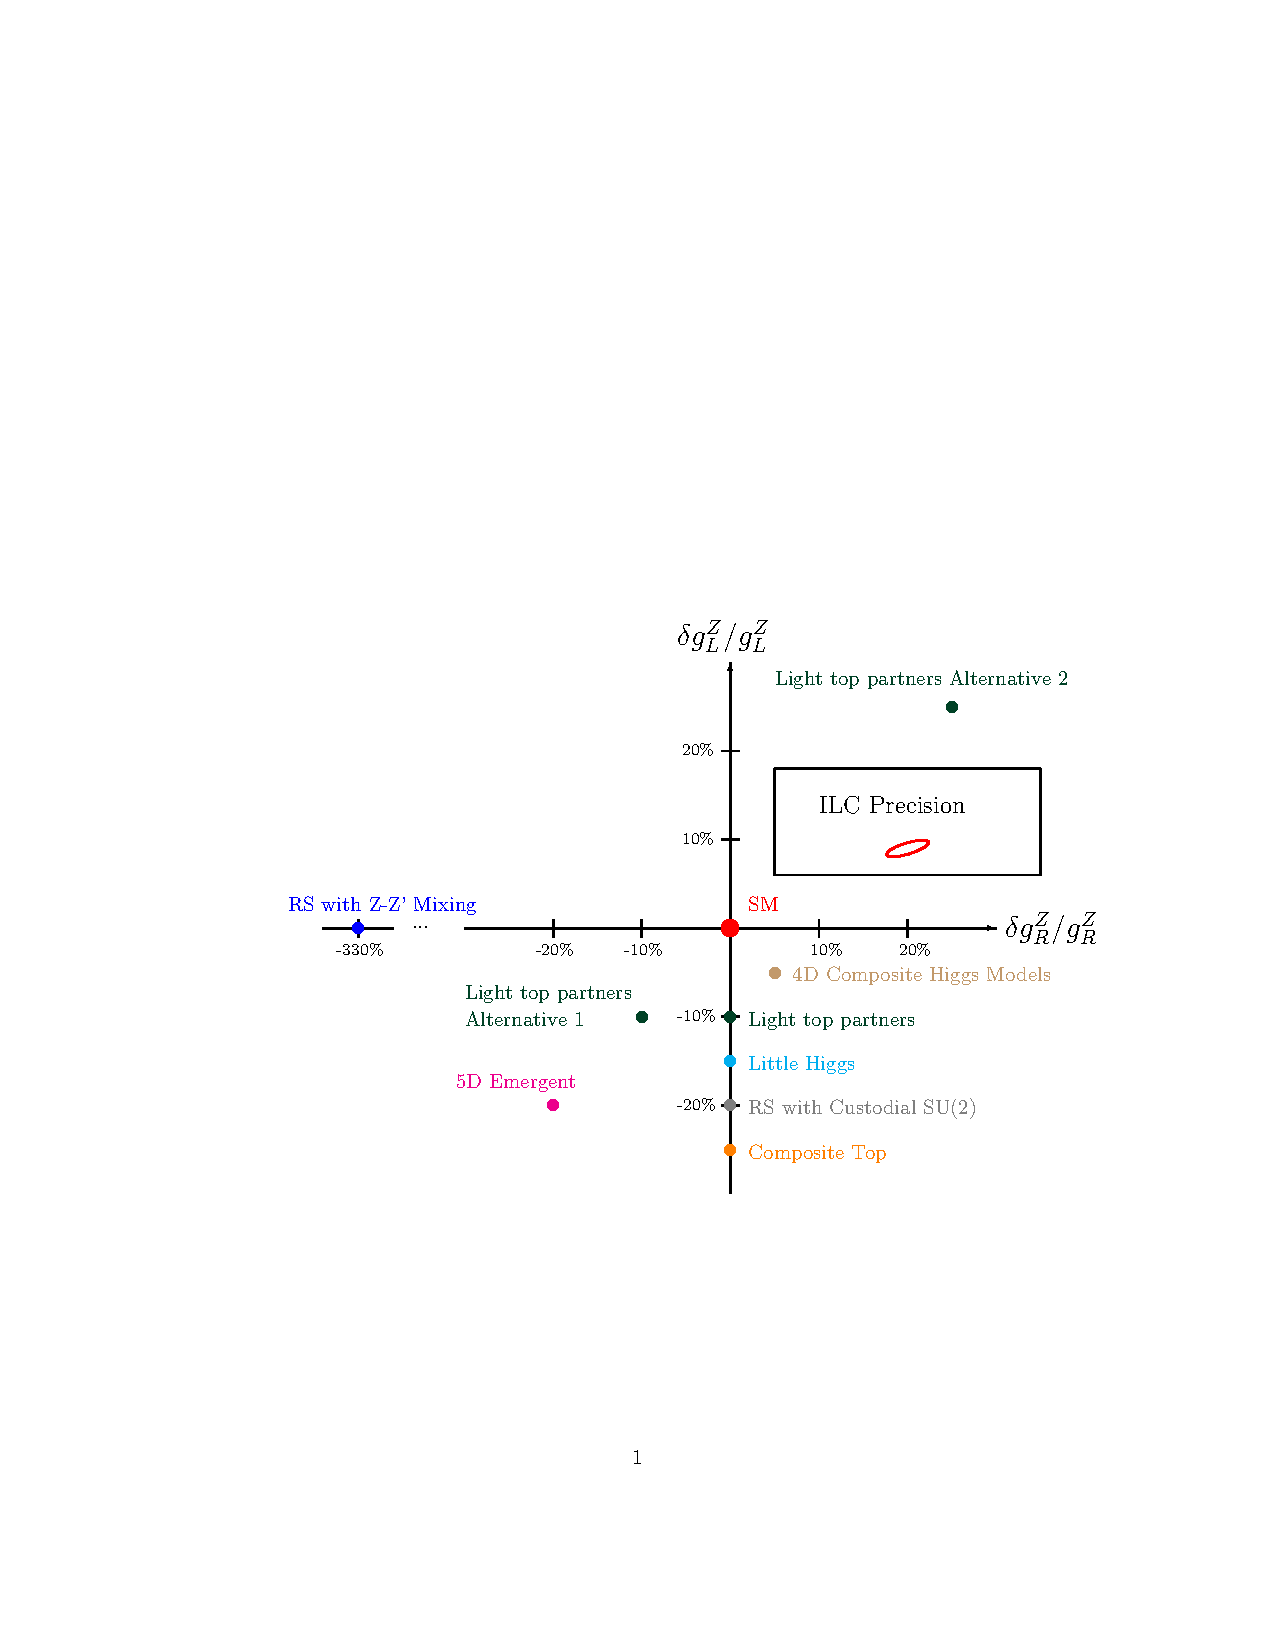
\includegraphics[clip, trim=4cm 7cm 2cm 10cm, width=0.95\textwidth]{ILD/graphics/plot.pdf}
		\caption{\sl Predictions of several models that incorporate Randall-Sundrum (RS) models and/or compositeness or Little Higgs models on the deviations of the left- and right-handed couplings of the $t$~quark to the $Z^0$ boson. The ellipse in the frame in the upper right corner indicates the precision that can be expected for the ILC running at a center-of-mass energy of $\sqrt[]{s} = 500\,GeV$ after having accumulated ${\mathcal L}=500\,fb^{-1}$ of integrated luminosity shared equally between the beam polarizations $P(e^-),\,P(e^+) =\pm0.8,\mp0.3$. The original version of this figure can be found in~\cite{bib:ILCTOP}.}
		\label{fig:DeviationsTop}
	}
\end{figure}

The relative deviations of the left-handed and right-handed couplings of the top quark are predicted by various BSM theories are shown in Fig.~\ref{fig:DeviationsTop}.
A precise measurement of the top quark couplings allows for identification of the particular BSM theory.
  
%Concerning the \bbbar\ channel, experiments with polarized beams have an advantage of sign flip detection of the right-handed coupling $g_R^Z$, which can be produced by the Randall-Sundrum models with $Z^0$-$Z'$ mixing~\cite{bib:RSTOP}.
%
%Many \bsm\ models predict deviations on the heavy quark couplings to the Higgs and weak bosons.


%\begin{figure}[H]
  \centering
\setlength{\unitlength}{1.5mm}
%\setlength{\unitlength}{\textwidth} 

\begin{picture}(150,90)
\linethickness{0.3mm}
%\begin{center}
%compose x axis
  \put(9,33){\line(0,1){2}}
  \put(5,34){\line(1,0){8}}  
  \put(15,34){...} 
  \put(21,34){\vector(1,0){60}} 
  \put(82,33){\Large{$\delta g^Z_R / g^Z_R$}}
  \multiput(31,33)(10,0){5}{\line(0,1){2}} 
  \put(6.5,31){\footnotesize{-330\%}} 
  \put(29,31){\footnotesize{-20\%}} 
  \put(39,31){\footnotesize{-10\%}}
  \put(60,31){\footnotesize{10\%}}
  \put(70,31){\footnotesize{20\%}}
%compose y-axis
  \put(51,4){\vector(0,1){60}} 
  \put(45,66){\Large{$\delta g^Z_L / g^Z_L$}}
  \multiput(50,14)(0,10){5}{\line(1,0){2}} 
  \put(45,13.5){\footnotesize{-20\%}} 
  \put(45,23.5){\footnotesize{-10\%}} 
  \put(45.5,43.5){\footnotesize{10\%}} 
  \put(45.5,53.5){\footnotesize{20\%}}
%Add models
  \put(51,34){\color{red}\circle*{2}} 
  \put(53,36){\color{red}SM}
  \put(51,24){\color{britishracinggreen}\circle*{1.5}}
  \put(53,23){\color{britishracinggreen}Light top partners~\cite{Grojean:2013qca}}
  \put(41,24){\color{britishracinggreen}\circle*{1.5}} 
  \put(21,26){\color{britishracinggreen} Light top partners}
 \put(21,23){\color{britishracinggreen} Alternative 1~\cite{bib:panico-priv}}
  \put(76,59){\color{britishracinggreen}\circle*{1.5}} 
  \put(56,61.5){\color{britishracinggreen} Light top partners Alternative 2~\cite{bib:panico-priv}}
  %\put(53,23){\color{green}Composite Higgs with SO(5)/SO(4)}%~\cite{Grojean:2013qca}}
   \put(51,19){\color{cyan}\circle*{1.5}} 
   \put(53,18){\color{cyan}Little Higgs~\cite{Berger:2005ht}}
  \put(51,14){\color{gray}\circle*{1.5}} 
  \put(53,13){\color{gray}RS with Custodial SU(2)~\cite{Carena:2006bn}}
  \put(51,9){\color{orange}\circle*{1.5}} 
  \put(53,8){\color{orange}Composite Top~\cite{Pomarol:2008bh}}
  \put(31,14){\color{magenta}\circle*{1.5}} 
  \put(20,16){\color{magenta}5D Emergent~\cite{Cui:2010ds}}
  \put(56,29){\color{camel}\circle*{1.5}} 
  \put(58,28){\color{camel}4D Composite Higgs Models~\cite{Barducci:2015aoa}}
  \put(9,34){\color{blue}\circle*{1.5}} 
  \put(1,36){\color{blue}RS with Z-Z' Mixing~\cite{Djouadi:2006rk}}
%make a box to put the ILC precision into
\multiput(56,40)(30,0){2}{\line(0,1){12}} 
\multiput(56,40)(0,12){2}{\line(1,0){30}}
\put(61,47){\large{ILC Precision}}
%embed the covariance ellipse
\color{red}
% Ellipse:  u = 71.0  v = 43.0  a = 2.45336  b = 0.631947  phi = 16.9866 Grad
\qbezier(73.3463, 43.7167)(73.2699, 43.9671)(72.5286, 43.9342)
\qbezier(72.5286, 43.9342)(71.7873, 43.9013)(70.8154, 43.6044)
\qbezier(70.8154, 43.6044)(69.8435, 43.3075)(69.2103, 42.9205)
\qbezier(69.2103, 42.9205)(68.5772, 42.5336)(68.6537, 42.2833)
\qbezier(68.6537, 42.2833)(68.7301, 42.0329)(69.4714, 42.0658)
\qbezier(69.4714, 42.0658)(70.2127, 42.0987)(71.1846, 42.3956)
\qbezier(71.1846, 42.3956)(72.1565, 42.6925)(72.7897, 43.0795)
\qbezier(72.7897, 43.0795)(73.4228, 43.4664)(73.3463, 43.7167)
\end{picture}





\caption{\sl Predictions of several models that incorporate Randall-Sundrum (RS) models and/or compositeness or Little Higgs models on the deviations of the left- and right-handed couplings of the $t$~quark to the $Z^0$ boson. The ellipse in the frame in the upper right corner indicates the precision that can be expected for the ILC running at a centre-of-mass energy of $\sqrt[]{s} = 500\,GeV$ after having accumulated ${\mathcal L}=500\,fb^{-1}$ of integrated luminosity shared equally between the beam polarisations $P(e^-),\,P(e^+) =\pm0.8,\mp0.3$. The original version of this figure can be found in~\cite{bib:ILCTOP}.}
\label{fig:models-rp}
\end{figure}
%Supersymmetric models  -  have different set of Higgs couplings to the up and down type quarks.
%%%%%%%%%%%%%%%%%%%%%%%%%%%%%%%%%%%%%%%%%%%%%%%%%%%%%%%%%%%%%%%%
%%%%%%%%%%%%%%%%%%%%%%%%%%%%%%%%%%%%%%%%%%%%%%%%%%%%%%%%%%%%%%%%
%%%%%%%%%%%%%%%%%%%%%%%%%%%%%%%%%%%%%%%%%%%%%%%%%%%%%%%%%%%%%%%%
\subsection{Status of the measurements and simulation studies}
%mass measurements

\subsubsection{Measurements at LEP and SLC}
%The electron-positron colliders have a large production cross section of $e^+e^- \to q\bar{q}$ process mediated by $Z^0$ boson or a virtual photon.
The total cross sections of various \sm\ processes for the $e^+e^-$ machines are shown in Fig.~\ref{fig:LCcrosssection}.

The circular LEP~I and the linear SLC colliders operated at the $Z^0$ pole, where the $e^+e^-$ cross section is maximal as seen from Fig.~\ref{fig:LCcrosssection}.
The measurements resulted in extremely precise b-quark fraction $R_b$ and the b-quark forward-backward asymmetry $A_{FB}^b$ measurements. 
The measured $R_b$ value, which is the ratio of b-quark cross section over total hadronic cross section, has full compatibility with the \sm\ prediction. 
On the other hand, the measured b-quark forward-backward asymmetry $A_{FB}^b$, dominated by the LEP~I precision, has 2.5\,$\sigma$ deviation with the recent electroweak fit predictions~\cite{bib:AfbSMFit}.
%The measurement of the $A_{FB}^b$ value at the SLC have 27\% higher uncertainty than the LEP results~\cite{bib:SLC}.

\begin{figure}[h]
	{\centering
		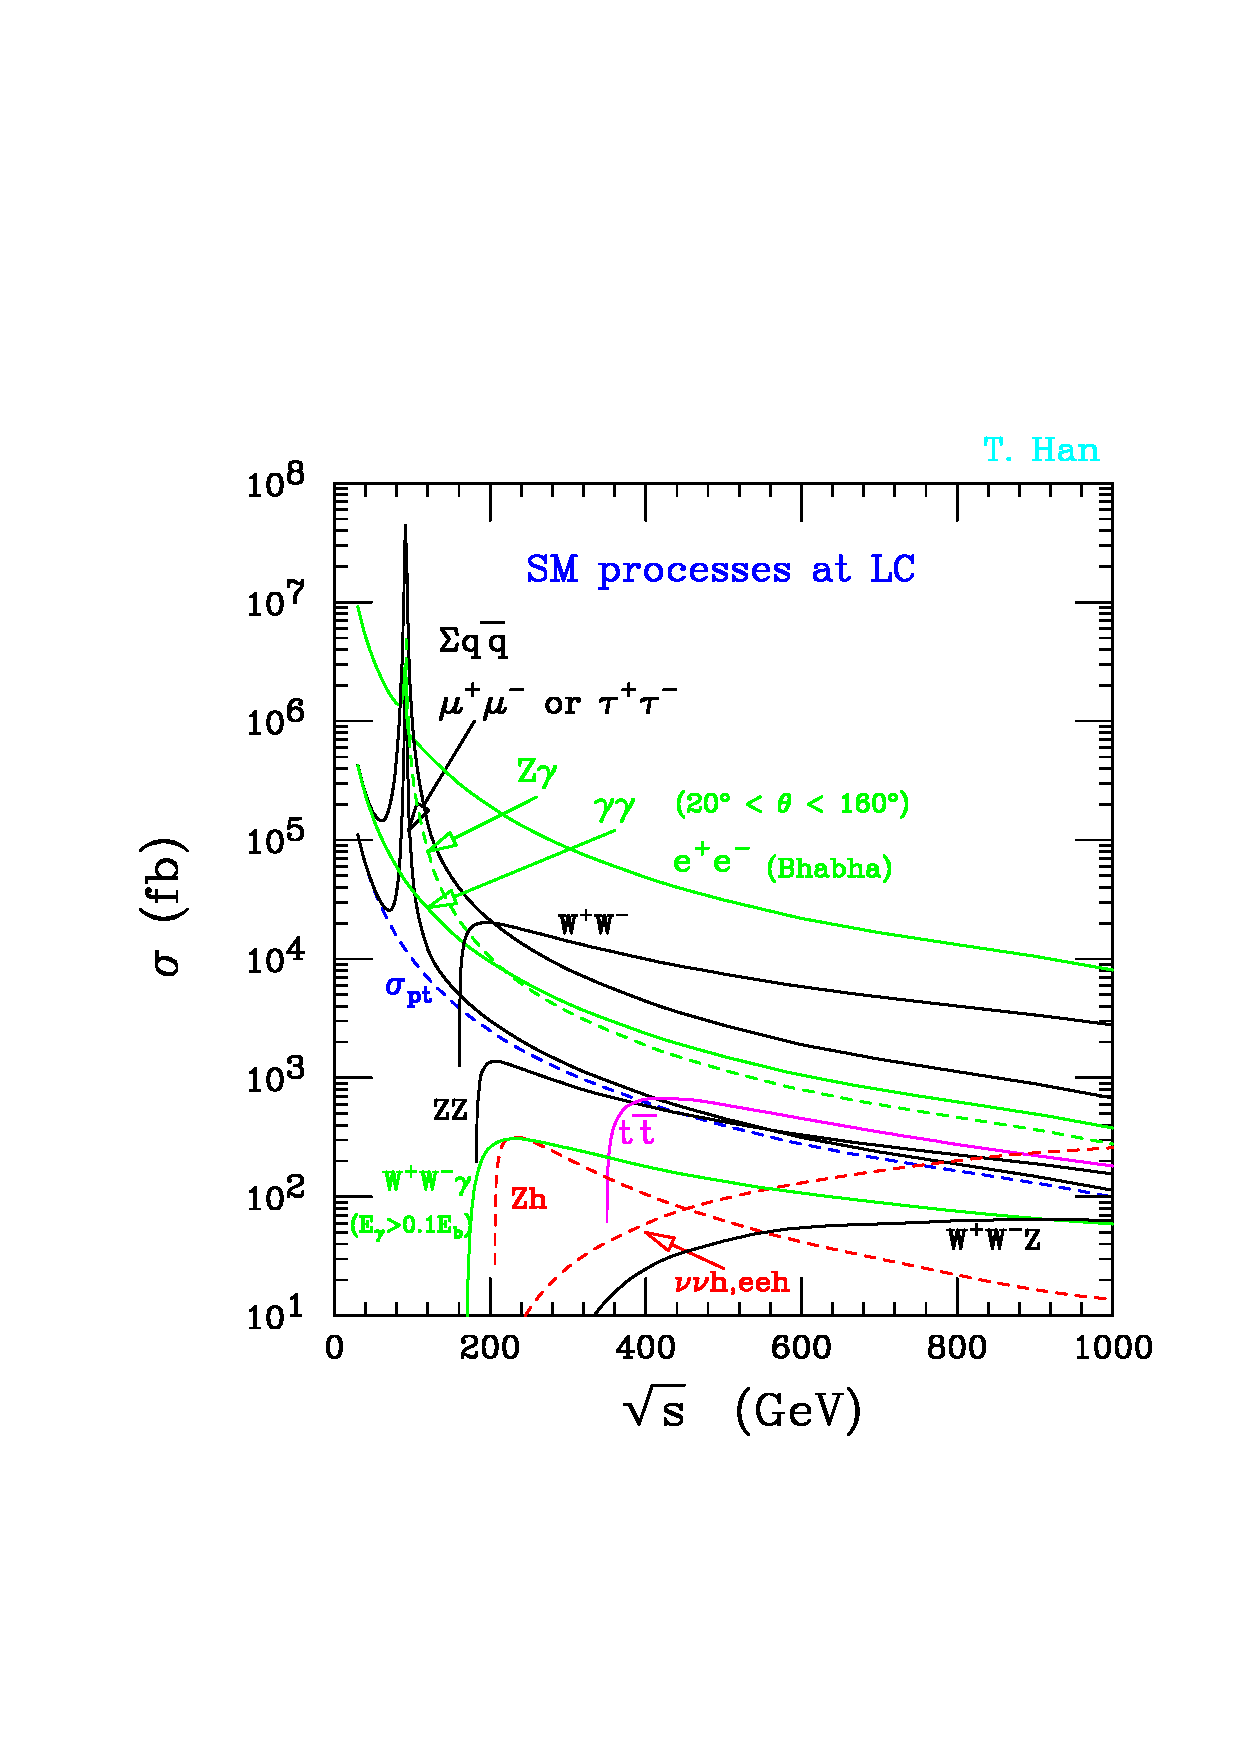
\includegraphics[clip, trim=0.5cm 5cm 0.5cm 7cm, width=0.95\textwidth]{ILD/graphics/epem_sm-hepph.pdf}
		\caption{\sl Tree-level cross sections of major \sm\ processes at linear colliders as function of center-of-mass energy assuming no polarization of the initial state~\cite{bib:Han}.}
		\label{fig:LCcrosssection}
	}
\end{figure}


The measurements outside $Z^0$ pole were carried out by the LEP~II programme, which collected the most integrated luminosity at around 190\,GeV energy, at the $W^\pm$-pair production threshold. 
The measured $A_{FB}^b$ at this center-of-mass energy agrees within 2\,$\sigma$ with the tree level \sm\ prediction.

The polarized initial state at the SLC allowed to introduce the left-right asymmetry $A(SLD)$.
This observable measures the difference between the left-handed and the right-handed initial state polarization cross sections. The measured value of the left-right asymmetry for leptons $A_l(SLD)$ has 2\,$\sigma$ deviation from the \sm\ prediction~\cite{bib:AfbSMFit}. The computed values of $\sin^2\theta_W$ using $A_{FB}^b$ from LEP and $A_l(SLD)$ differ significantly.

The precise determination of the $Zb\bar{b}$ vertex at LEP~I and SLC experiments allowed to put constraints on the top quark and Higgs boson masses.
The LEP measurement allowed to predict the top quark mass in the region of 133\,GeV $ < m_t < $ 190\,GeV and the Higgs boson mass  10\,GeV $< m_H <$ 440\,GeV~\cite{bib:LEPTOP}, which were later confirmed by the TeVatron and the LHC experiments. 
%$A_{fb}^b(\sqrt[]{s} = 190.7\,\text{GeV})=0.51\pm0.058$
%Unfortunately, the beam energies of LEP~II and SLC was not high enough to produce single top or top quark pairs, therefore, the precise determination of the top electroweak couplings is left for the future electron-positron machines.

\subsubsection{LHC and TeVatron measurements}
The composite nature of colliding particles at the hadron colliders priviledges the production of the top quark pairs through the strong interaction via high cross section $gg\to t\bar{t}$ or $q\bar{q}\to t\bar{t}$ processes.
Therefore, the hadron machines can measure the top mass as the cross section parameter with a high precision. 

The TeVatron has a high production rate of the single top-quark via $q\bar{q}' \to W^\pm \to t\bar{b}$ process. %at a higher rate than proton-proton machines. 
This process involve $tbW$ vertex and therefore, its total cross section depends on the weak couplings of the top quark. 
The measurement of the single top cross section at TeVatron is found to be consistent with the \sm\ predictions~\cite{bib:TeVstop} with about 16\% uncertainty.

The measurements of the forward-backward asymmetry at TeVatron~\cite{bib:TeVAfb} and the charge asymmetry at the LHC~\cite{Naranjo:2017etb} of the strong $t\bar{t}$ production are consistent with the \sm\ expectations. 

To measure the electroweak couplings of the top quark at the LHC, the associate production of top quark pair with $Z^0$ or $W^\pm$ bosons is required, which has a lower cross section, than the \ttbar\ production process.
Study of the $t\bar{t}Z^0$ process has been done at the LHC experiments using Run I data with $\sqrt{s} = 8$\,TeV. It shows compatible rates of the signal process with the \sm, but more statistics is required to measure the cross section precisely~\cite{bib:CMSttz2014}. The cross section fit results for the $t\bar{t}Z^0$ and $t\bar{t}W^\pm$ processes are shown in Fig~\ref{fig:LCHTopTopZ_3}.
Including the Run~II data of the LHC with a higher center-of-mass energy will significantly improve $t\bar{t}Z^0$ measurement.
%Main channel of the top quark production is gluons
\begin{figure}[h]
	{\centering
		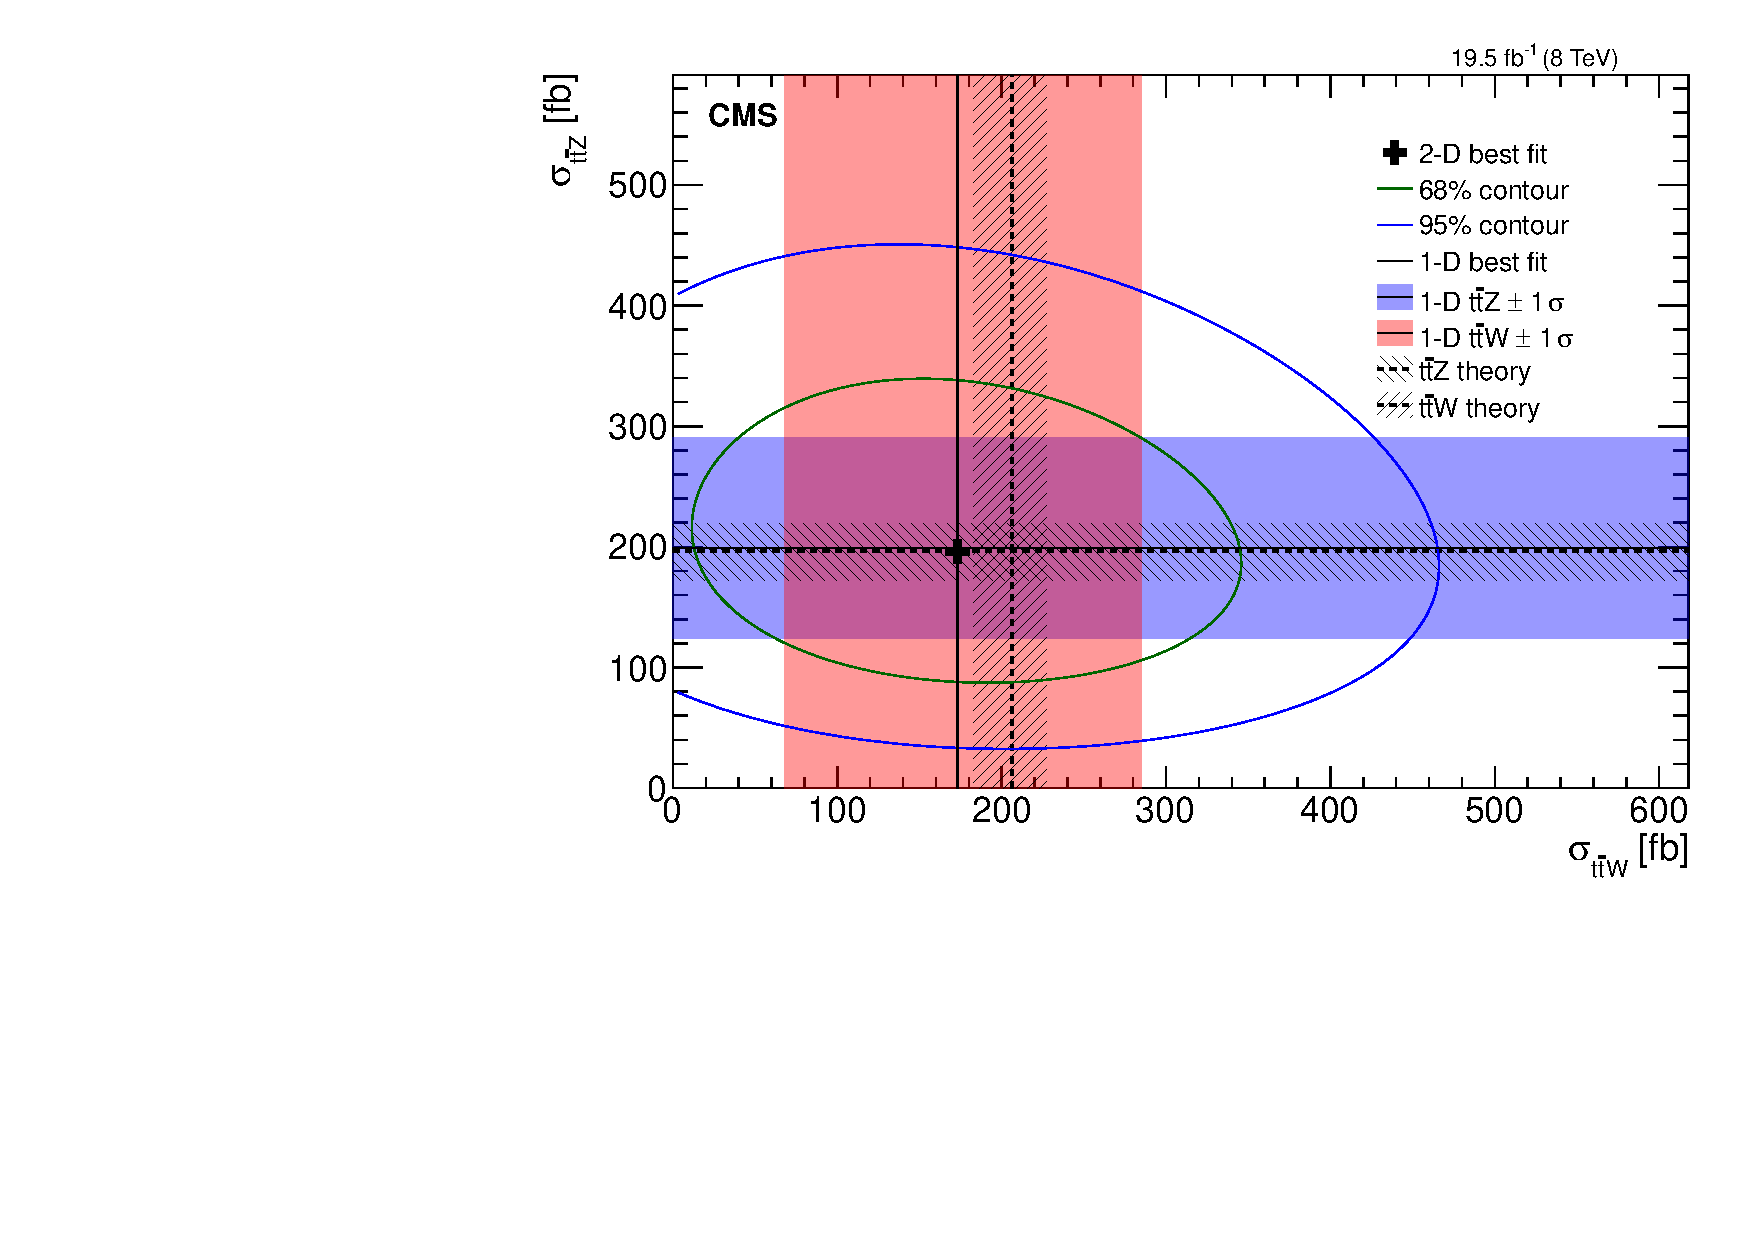
\includegraphics[ width=0.55\textwidth]{ILD/graphics/fit_2d.pdf}
		\caption{\sl The result of the two-dimensional best fit for $t\bar{t}W^\pm$ and $t\bar{t}Z^0$ cross sections (cross symbol) is shown along with its 68 and 95\% confidence level contours by the CMS experiment. The result of this fit is superimposed with the separate $t\bar{t}W^\pm$ and $t\bar{t}Z^0$ cross section measurements, and the corresponding 1 standard deviation (1\,$\sigma$) bands, obtained from the dilepton, and the trilepton/four-lepton channels, respectively. The figure also shows the predictions from theory and the corresponding uncertainties.~\cite{bib:CMSttz2014}.}
		\label{fig:LCHTopTopZ_3}
	}
\end{figure}
%ttZ cross section measurements

The study of the b-quark electroweak couplings is very limited at hadron colliders.
The possible $Z^0b\bar{b}$ associate production study at the LHC can provide only the cross section magnitude value, which has been measured at LEP~I to have no deviation from the \sm\ prediction. 
Top quark have never been studied at the $e^+e^-$ colliders, benefiting from a direct electroweak production and a high signal over background ratio.
Hence, precise measurements of the heavy quark electroweak couplings are left for future $e^+e^-$ machines.




%2.5s tension by LEP in bbar asymmetry
\subsubsection{Future linear colliders}

The acceleration technologies available today allow for the construction and the running of a linear electron-positron collider at center-of-mass energies well above top pair production threshold. The clean environment of the linear colliders allows detection and reconstruction of all \sm\ decay modes of the top quark: fully leptonic, semileptonic and fully hadronic decays. 



As can be seen from expression of the differential cross section~(\ref{formula:DiffSigma_3}), the sensitivity to axial form factors is proportional to the fermion velocity $\beta$, therefore, the higher beam energies, like 500\,GeV stage at the ILC are preferred for a study of electroweak top quark couplings. 
The b-quark coupling analysis can be done at all center-of-mass energies, scheduled at the ILC project.


%Matrix element method fully leptonic
%Such assets of the future $e^+e^-$ colliders as high signal-to-noise ratio and high-granularity of the detectors allow to use Matrix Element Method to compute the form factors from a kinematical fit of the top pair decay products. 
%This method can be applied at the ILC for fully leptonic decay of the top quark pair. 

The first top quark electroweak coupling analysis at the ILC was published in Ref.~\cite{bib:ILCTOP}, where the uncertainties on the form factors (\ref{formula:SMformFactors_3}) and the couplings (\ref{formula:EWcouplings_3}) were estimated using the ILD environment.


The semileptonic top decays were used in~\cite{bib:ILCTOP}, where  a lepton from leptonic top quark decay $t\to b l \bar{\nu_l}$ provides the charge information, and jets from hadronic top quark decays $t \to b q \bar{q}'$ are used for top polar angle reconstruction. 
It was found that, an accidental assignment of the hadronic $W^\pm$ jets to the b-jet from leptonic top quark decays can happen. This mistake 
amounts to flip the value of $\cos\theta_{top}$ into $-\cos\theta_{top}$, which lead to a large deviation from the generated polar angle distribution, as shown in Fig.~\ref{fig:ILCTOPAFB_a_3}.
This effect is called an event migration problem.
Only the left-handed electron beam distribution is affected due to the $W^\pm$ boson kinematics, as explained in~\cite{bib:ILCTOP}. 
%CLIC

The study of the electroweak top couplings at CLIC was done at $\sqrt{s} = 380$\,GeV~\cite{bib:Garcia}. This study confirms the event migration effect.


There are two possible ways to remedy the migration effect problem - by doing a kinematical cut on $\chi^2_{top}$, which is a measure of hadronic top reconstruction quality, or by finding a correct combination of lepton charge with the b-quark charge. 
The main advantage of the combination with the b-quark charge is that this method do not require precise knowledge of the top quark decay kinematics, as it is needed for the $\chi^2_{top}$ cut method. 
The reconstructed top polar angle distribution for semileptonic decay of the top quark pair is shown in Fig.~\ref{fig:ILCTOPAFB}, where one sees the $W^\pm$ lepton migration effect caused by the $W^\pm$ kinematics and the resolution of the problem by the kinematical cut on $\chi^2_{top}$ in Fig.~\ref{fig:ILCTOPAFB_b_3}.


\begin{figure}[H]
	\centering
	\begin{subfigure}{0.5\textwidth}
		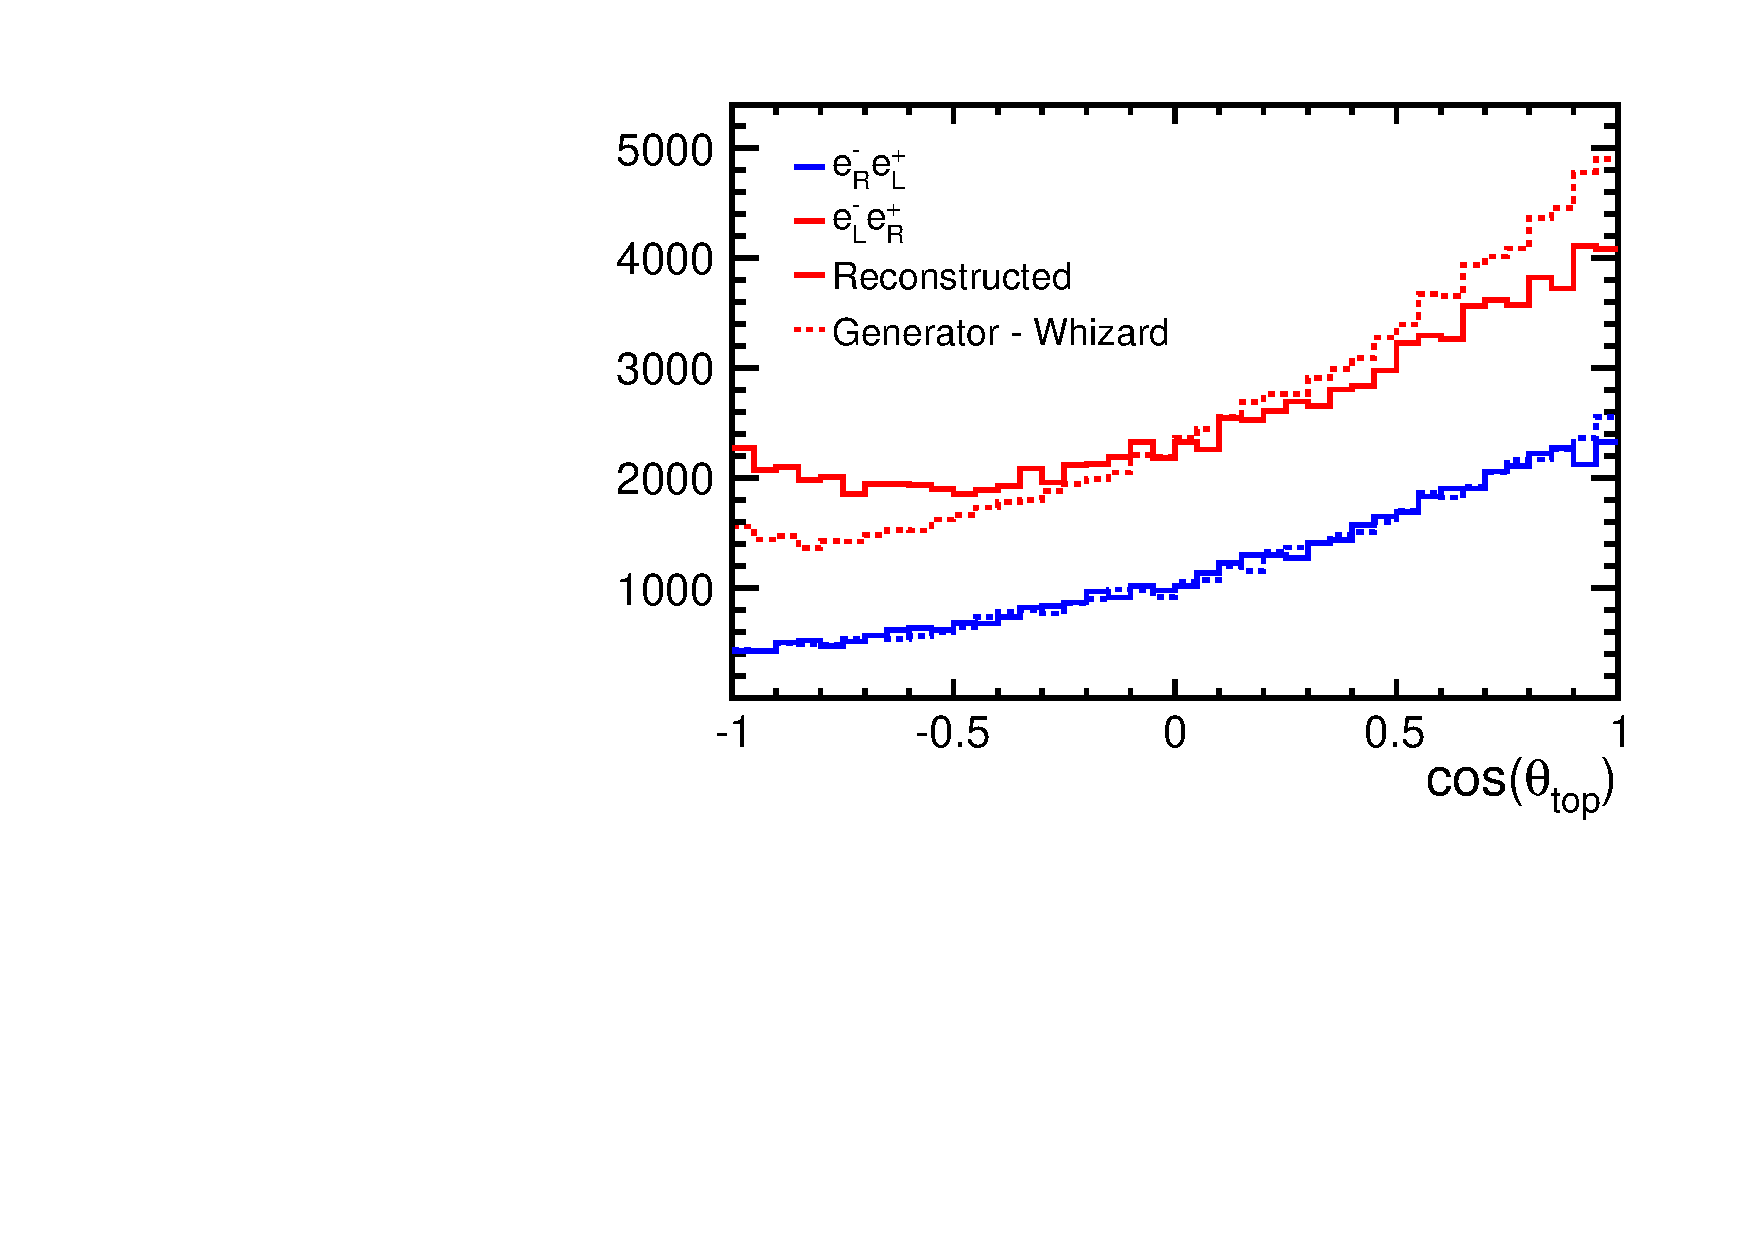
\includegraphics[clip, trim=0.9cm 0cm 0.9cm 0cm,width=0.99\textwidth]{ILD/graphics/EPS_AFB_nocut.pdf}
		\caption{\label{fig:ILCTOPAFB_a_3} }
	\end{subfigure}% 
	\begin{subfigure}{0.5\textwidth}
		\centering
		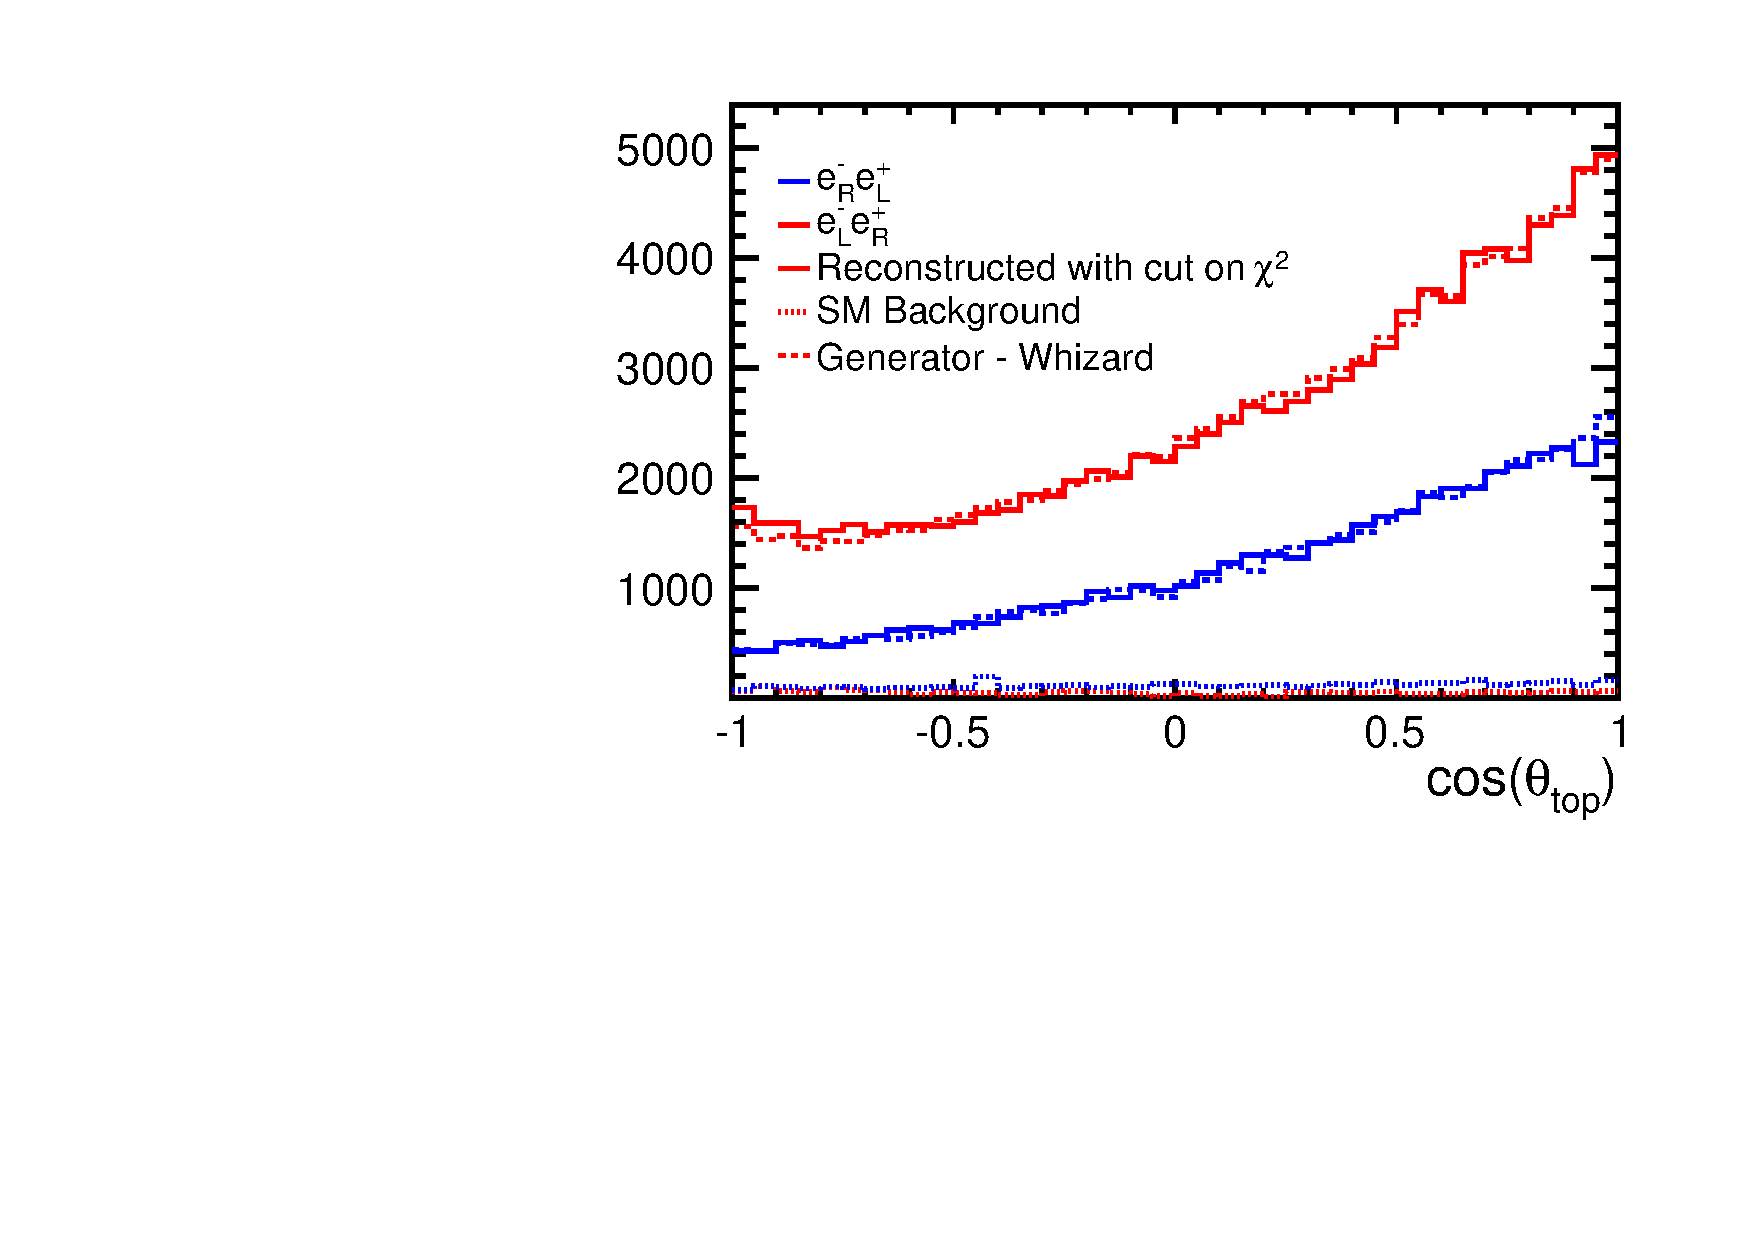
\includegraphics[clip, trim=0.9cm 0cm 0.9cm 0cm,width=0.99\textwidth]{ILD/graphics/AFB_wbkg_chi2cut.pdf}
		\caption{\label{fig:ILCTOPAFB_b_3} }
	\end{subfigure}
	\caption{\sl Reconstructed top quark polar angle before (a) and after $\chi^2_{top}$ cut (b) distributions compared with the prediction by the event generator for two configurations of the beam polarizations~\cite{bib:ILCTOP}. }
	
	\label{fig:ILCTOPAFB}
\end{figure}

The first attempt to use the quark charge technique in fully hadronic \ttbar\ decays was done by~\cite{amjad:tel-00949818}, but it required large simulation-dependent corrections. 
Hence, one needs to investigate the reasons of inefficiency and impurity of the quark charge measurement in the ILD environment and propose a method to fix the problems. 



The development of the b-quark charge measurement will increase the statistics for semileptonic \ttbar\ channel,  open access to the fully hadronic \ttbar\ decay channels without any Monte-Carlo corrections and, moreover, it will allow a study of electroweak coupling of the bottom quark, which have never been done using the ILC environment. 


%Study of precision of ILC on top couplings were made by Amjad et al. using semileptonic decays. 
%Central problem: migration effect of the lepton from W. 
%B charge was first used as a way to remove migration effect by Jeremy for semileptonic channel.  and Amjad for hadronic one. 
%Development of quark charge measurement technique willl increase the statistics for semileptonic channel, and open hadronic top decays. 
%The quark charge measurement is the only way to study the bbbar process.  

%%%%%%%%%%%%%%%%%%%%%%%%%%%%%%%%%%%%%%%%%%%%%%%%
%%%%%%%%%%%%%%%%%%%%%%%%%%%%%%%%%%%%%%%%%%%%%%%%
%%%%%%%%%%%%%%%%%%%%%%%%%%%%%%%%%%%%%%%%%%%%%%%%

\section{B-quark charge reconstruction}
\label{sec:JetChargeReconstruction}
An information about the bottom quark charge is useful for all \sm\ processes, where b-jets appear as decay products. 
In this thesis it is used for quark polar angle reconstruction of $e^+e^-\to t\bar{t}$ and $e^+e^- \to b\bar{b}$ processes. 
The polar angle spectrum is used to determine the quark couplings. 
This requires a high purity and a high efficiency of the b-quark charge reconstruction, which is an ultimate challenge for every reconstruction algorithm and all subdetectors of the experiment. 

One of the main goals of this thesis is to develop a method of the b-quark charge measurement with high purity and efficiency using the full simulation of the ILD experiment. 
To do so, first, it is necessary to measure the performance of the standard reconstruction algorithm and find sources of charge impurities, and then develop an algorithm to improve it. 


%%%%%%%%%%%%%%%%%%%%%%%%%%%%%%%%%%%%%%%%%%%%%%%%%%%%%%%%%%%
%%%%%%%%%%%%%%%%%%%%%%%%%%%%%%%%%%%%%%%%%%%%%%%%%%%%%%%%%%%
%%%%%%%%%%%%%%%%%%%%%%%%%%%%%%%%%%%%%%%%%%%%%%%%%%%%%%%%%%%
\subsection{Setup of the study}

All studies in this and the next chapters are done using full simulation of the baseline ILD experiment. 
The b-quark charge measurement study uses $e^+e^- \to b\bar{b}$ at $\sqrt[]{s} = 250$\,GeV and the semileptonic decay mode of the $e^+e^- \to t\bar{t}$ at $\sqrt[]{s} = 500$\,GeV processes generated using {\sc whizard}~1.95 event generator. 
The hadronization of the quarks and gluons is done by the {\sc pythia}~6.205 event generator.
The distributions of the b-hadron momentum, generated by {\sc pythia} for the 250\,GeV $b\bar{b}$ and the 500\,GeV $t\bar{t}$ pairs are shown in Fig.~\ref{fig:GenHadronMomentum_3}. 
The distributions have different peak energies, bur the energy range is the same. Further analysis shows, that this difference has small impact on the performance of the quark charge reconstruction.
\begin{figure}[h]
	{\centering
		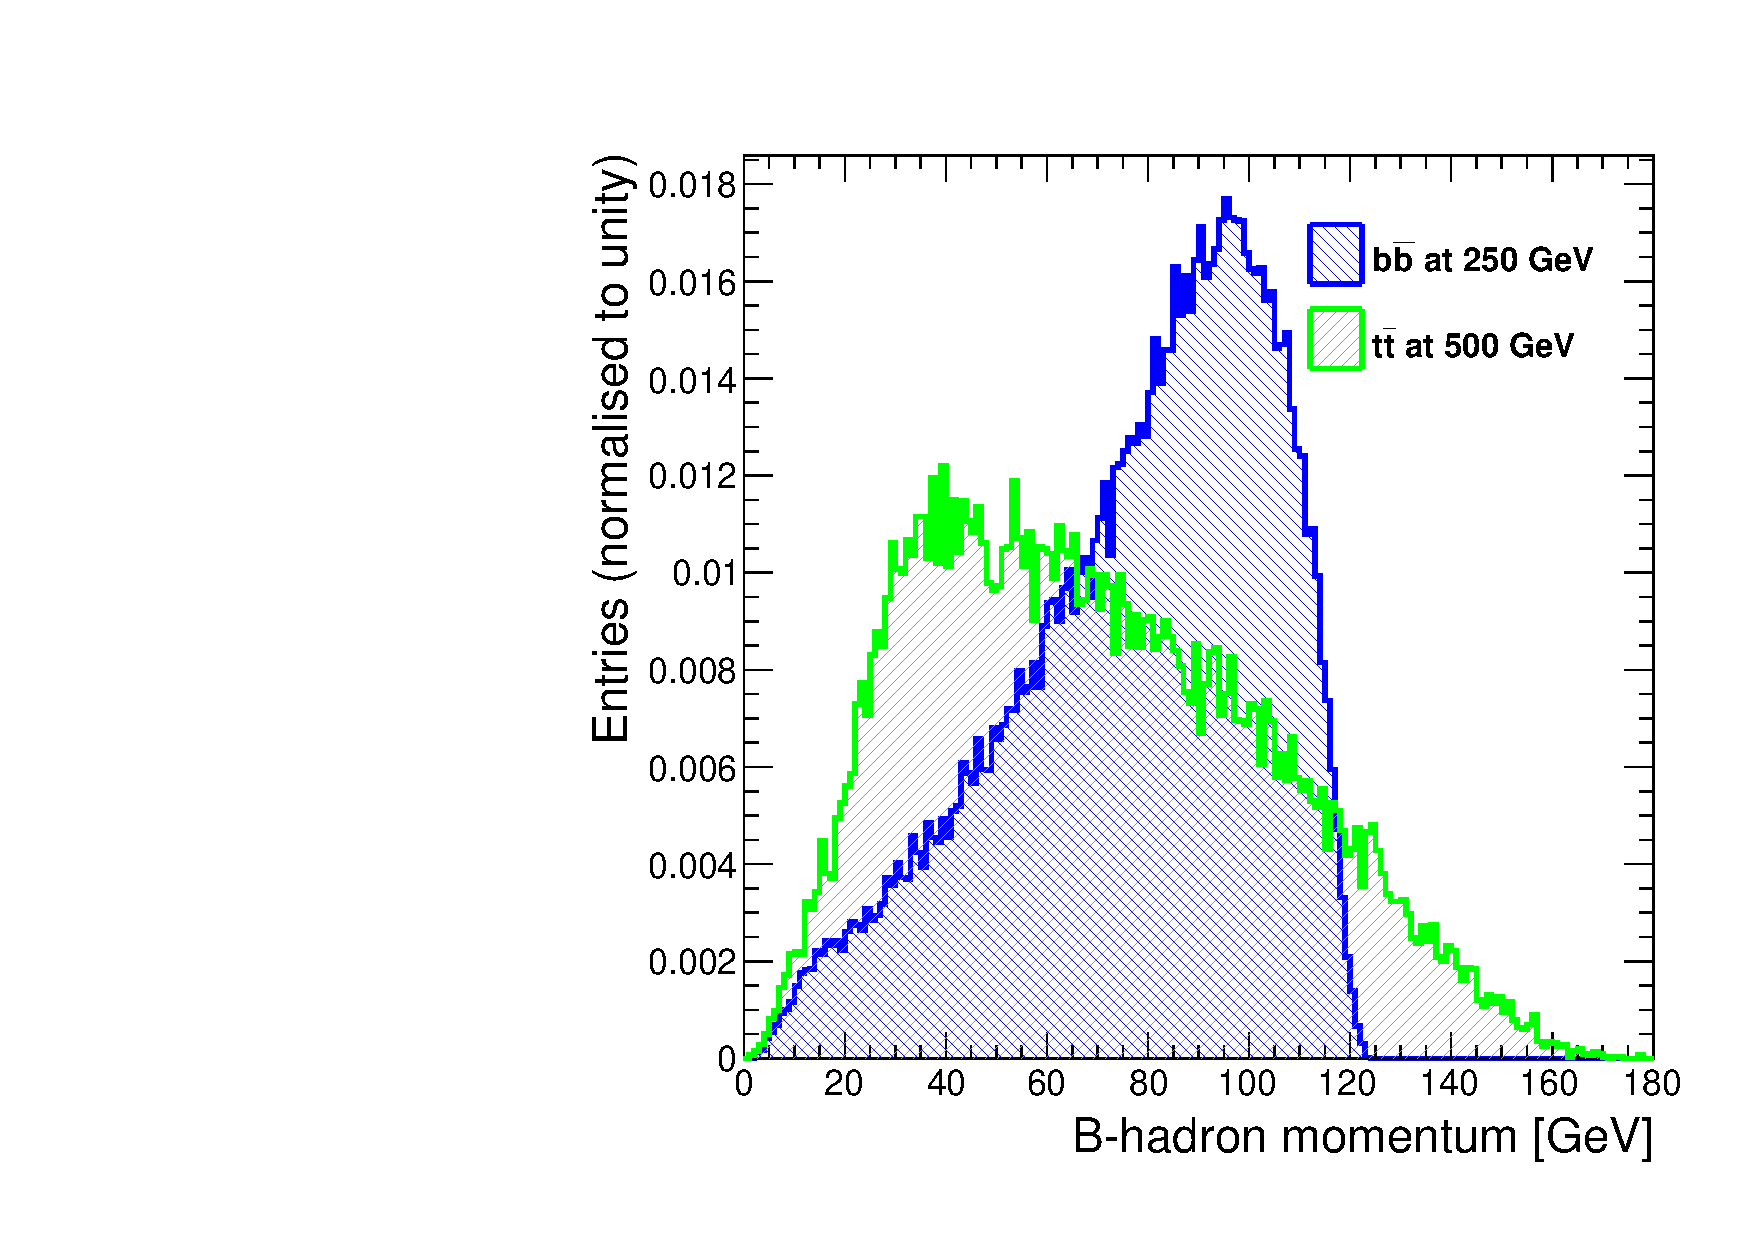
\includegraphics[width=0.45\textwidth]{ILD/plots/gen-hadron-momentum.pdf}
		\caption{\sl Generated b-hadron momentum by {\sc pythia} for \bbbar\ and \ttbar\ pair production processes signal processes.}
		\label{fig:GenHadronMomentum_3}
	}
\end{figure}

The $B^0-\bar{B}^0$ oscillations are enabled in the {\sc pythia} simulation. 
The ILD detector layout, the interaction of particles with the detector material and the detector response are simulated by the {\sc mokka} framework, that provides the geometry interface to the \geant\ toolkit. 

All reconstruction algorithms, along with the {\sc mokka} framework are part of the {\sc ilcsoft} software toolkit.
The modular structure of the {\sc ilcsoft} allows for independent execution of each reconstruction algorithm. 

%The ILD collaboration defines the order of the standard reconstruction chain, which is applied to all studies done using the full simulation of the ILD experiment. 

The most relevant standard reconstruction algorithms of the {\sc ilcsoft} for the b-quark charge measurement are described below:
\begin{itemize}
\item The MarlinTrk package organizes the hits, created by particles in the ILD trackers into reconstructed tracks. The track parametrization in described in~\cite{bib:LCIOtrack}. 
\item The PandoraPFA package is responsible for the clusterization of the calorimeter hits and creation of the Particle Flow Objects. The track covariance matrix is used to compute the covariance matrix of the reconstructed particle momentum; 
\item The primary and secondary vertex reconstruction is done by the Linear Collider Flavour Identification Plus or LCFI+ algorithm~\cite{bib:LCFI}. 
\end{itemize}
Each reconstructed track by the MarlinTrk algorithm has 5 parameters and the corresponding associated covariance matrix with 15 parameters; The most important for the thesis are the impact parameters $d_0$ and $z_0$, which are the transverse and longitudinal distance between the point of the closest approach to the reference point $(0,0)$, respectively. The corresponding uncertainties are $\sigma_{d_0}$ and $\sigma_{z_0}$, respectively.

The jet clustering algorithms can be configured and launched according to the analysis requirements. 
The flavor-tagging at the ILD experiment will serve to separate out jets from bottom and charm quarks from the light quark or gluon jets, the corresponding separation variables are called b- and c-tagging, respectively. 
The flavor-tagging algorithm within the LCFI+ package provides  b- and c-tagging information for each reconstructed jet.


%%%%%%%%%%%%%%%%%%%%%%%%%%%%%%%%%%%%%%%%%%%%%%%%%%%%%%%%%
%%%%%%%%%%%%%%%%%%%%%%%%%%%%%%%%%%%%%%%%%%%%%%%%%%%%%%%%%
%%%%%%%%%%%%%%%%%%%%%%%%%%%%%%%%%%%%%%%%%%%%%%%%%%%%%%%%%
\subsection{Bottom quark topology}

The charge of the b-quark can be derived from the properties of the b-hadron and its decay products. 
%Therefore, one needs to know precisely the properties of the underlying hadrons. 


The b-quark hadronization modes are displayed in Table~\ref{table:bhadrons}.
        \begin{table}[H]
        \begin{center}
        \begin{tabular}{l c c }
        \hline
        			& Branching ratio & $c\tau$ \\
        \hline
            \Bm\ meson & $40.4 \pm 0.6 $\% & 450\,$\mu$m \\
            \Bz\ meson & $40.4 \pm 0.6 $\% & 455.4\,$\mu$m  \\

            \Bzs\ meson & $10.3 \pm 0.5 $\% & 453.3\,$\mu$m   \\
         \hline
            b-baryon & $8.9 \pm 1.3 $\% & $\approx$ 447\,$\mu$m  \\

        \hline
        \end{tabular}
        \end{center}
        \caption{\sl Hadronization modes of the b-quark~\cite{bib:PDG}. }
        \label{table:bhadrons}
        \end{table}

These branching fractions are approximate and may have a dependency on the initial and final state kinematic and production environment~\cite{bib:PDG}.
However, the presence of the \Bzs\ meson increase the number of the neutral hadronization modes, which will cause additional complications for the charge measurement. 
The illustration of the b-quark hadronization and common decay modes are given in Fig.~\ref{fig:Bmodes_3}.
\begin{figure}[h]
	{\centering
		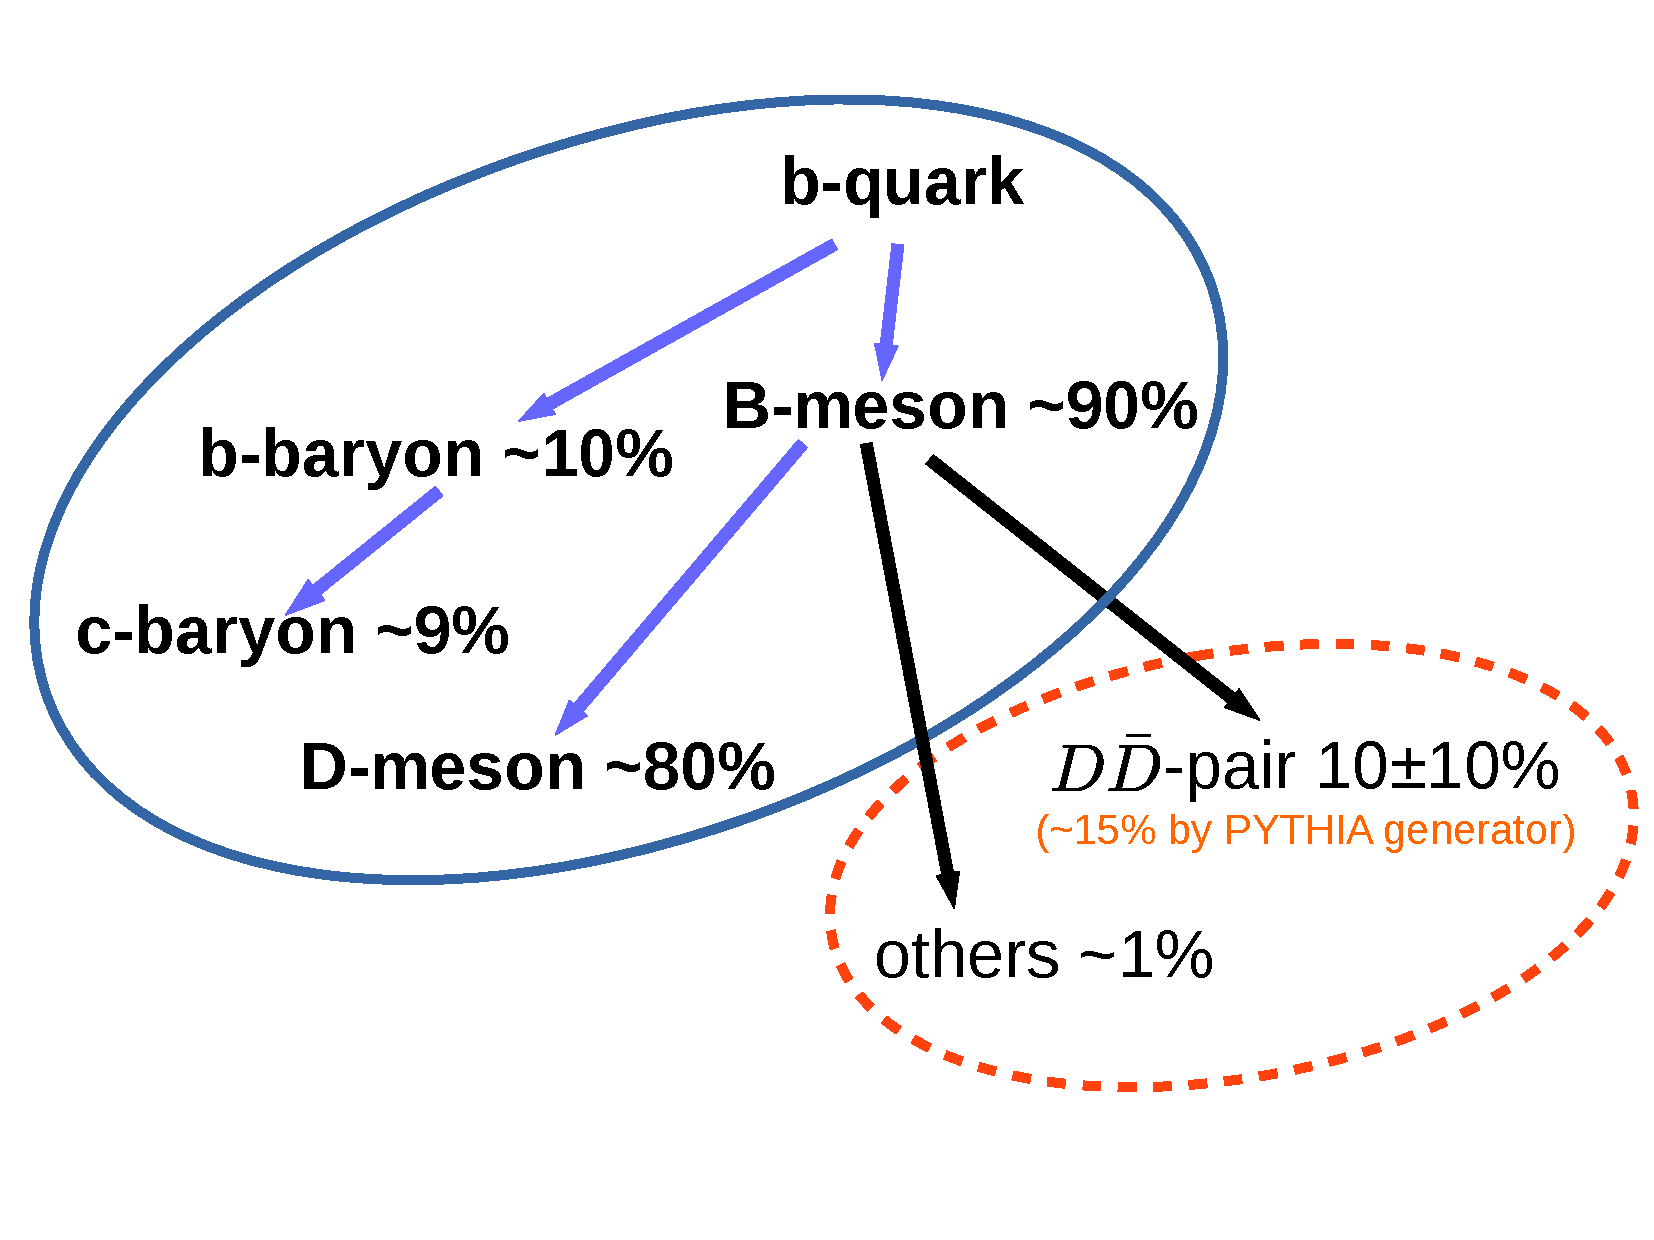
\includegraphics[width=0.55\textwidth]{ILD/plots/b-modes}
		\caption{\sl The illustration of the b-quark hadronisation and decay modes with the corresponiding decay rates in percent. Modes in the red circle are not tracked by the TruthVertexFinder.}
		\label{fig:Bmodes_3}
	}
\end{figure}

%b-hadron decays, typically, the charged pions, kaons, leptons or protons, 
Due to the Lorentz boost given by the initial b-quark energy, the b-hadron can travel several millimeters before its decay. Due to this flight distance, the charged particles from the b-hadron decays will have an offset with respect to the primary interaction point, which is the main signature of the b-quark jets. 

%Therefore we expect two vertices
The B meson have $D^0$ or $D^\pm$ meson decay modes of about 80\% decay rate, mediated by the weak interaction. The charmed $D$ mesons have a mean lifetime of $c\tau \approx 120 - 300$\,$\mu$m, which gives a possibility to the charmed mesons to travel away from the initial B meson decay vertex. 
Hence, one expects to detect two vertices from one b-jet in most of the cases: the secondary, which corresponds to the b-hadron decay, and the tertiary vertex created by the c-hadron decays. 

The $K^\pm$ mesons from B meson decays are the end products of the $b\to c\to s$ decay chain mediated by the weak interaction. 
The $K^\pm$ mesons have a long lifetime with $c\tau = 3.7$\,m and a high mass of 493.6\,MeV comparing with another long-lived charged particles from the B meson decays, like pions or leptons. 
Hence, it is possible to identify kaons by their energy deposition in the detector, which depend on particle mass. 
In the generator, about 87\% of b-hadrons are set to have correlated $K^\pm$ charge in the generator, which makes the $K^\pm$ charge a reliable indication of the initial b-quark charge. The kaon charge was used to determine the b-quark charge at the SLC~\cite{Falciai:1996jv} and the LEP experiments~\cite{Abreu:1999ui}.
On contrary, the b-baryons tend to produce protons, which have an opposite sign of charge to the initial b-quark charge.

%%%%%%%%%%%%%%%%%%%%%%%%%%%%%%%%%%%%%%%%%%%%%%%%%%%%%%%
%%%%%%%%%%%%%%%%%%%%%%%%%%%%%%%%%%%%%%%%%%%%%%%%%%%%%%%
%%%%%%%%%%%%%%%%%%%%%%%%%%%%%%%%%%%%%%%%%%%%%%%%%%%%%%%
\subsubsection{Generated vertices}
The output of the event generators is a list of generated particles with parent-child relations. 
The TruthVertexFinder algorithm was developed to find the generated vertices.%, and included into the {\sc ilcsoft} distribution. 
This algorithm detects the generated b-hadrons, finds the related charged particles, which can leave reconstructable tracks and organizes them into the generated secondary or tertiary vertices.



\begin{figure}
	\centering
	\begin{subfigure}{0.5\textwidth}
		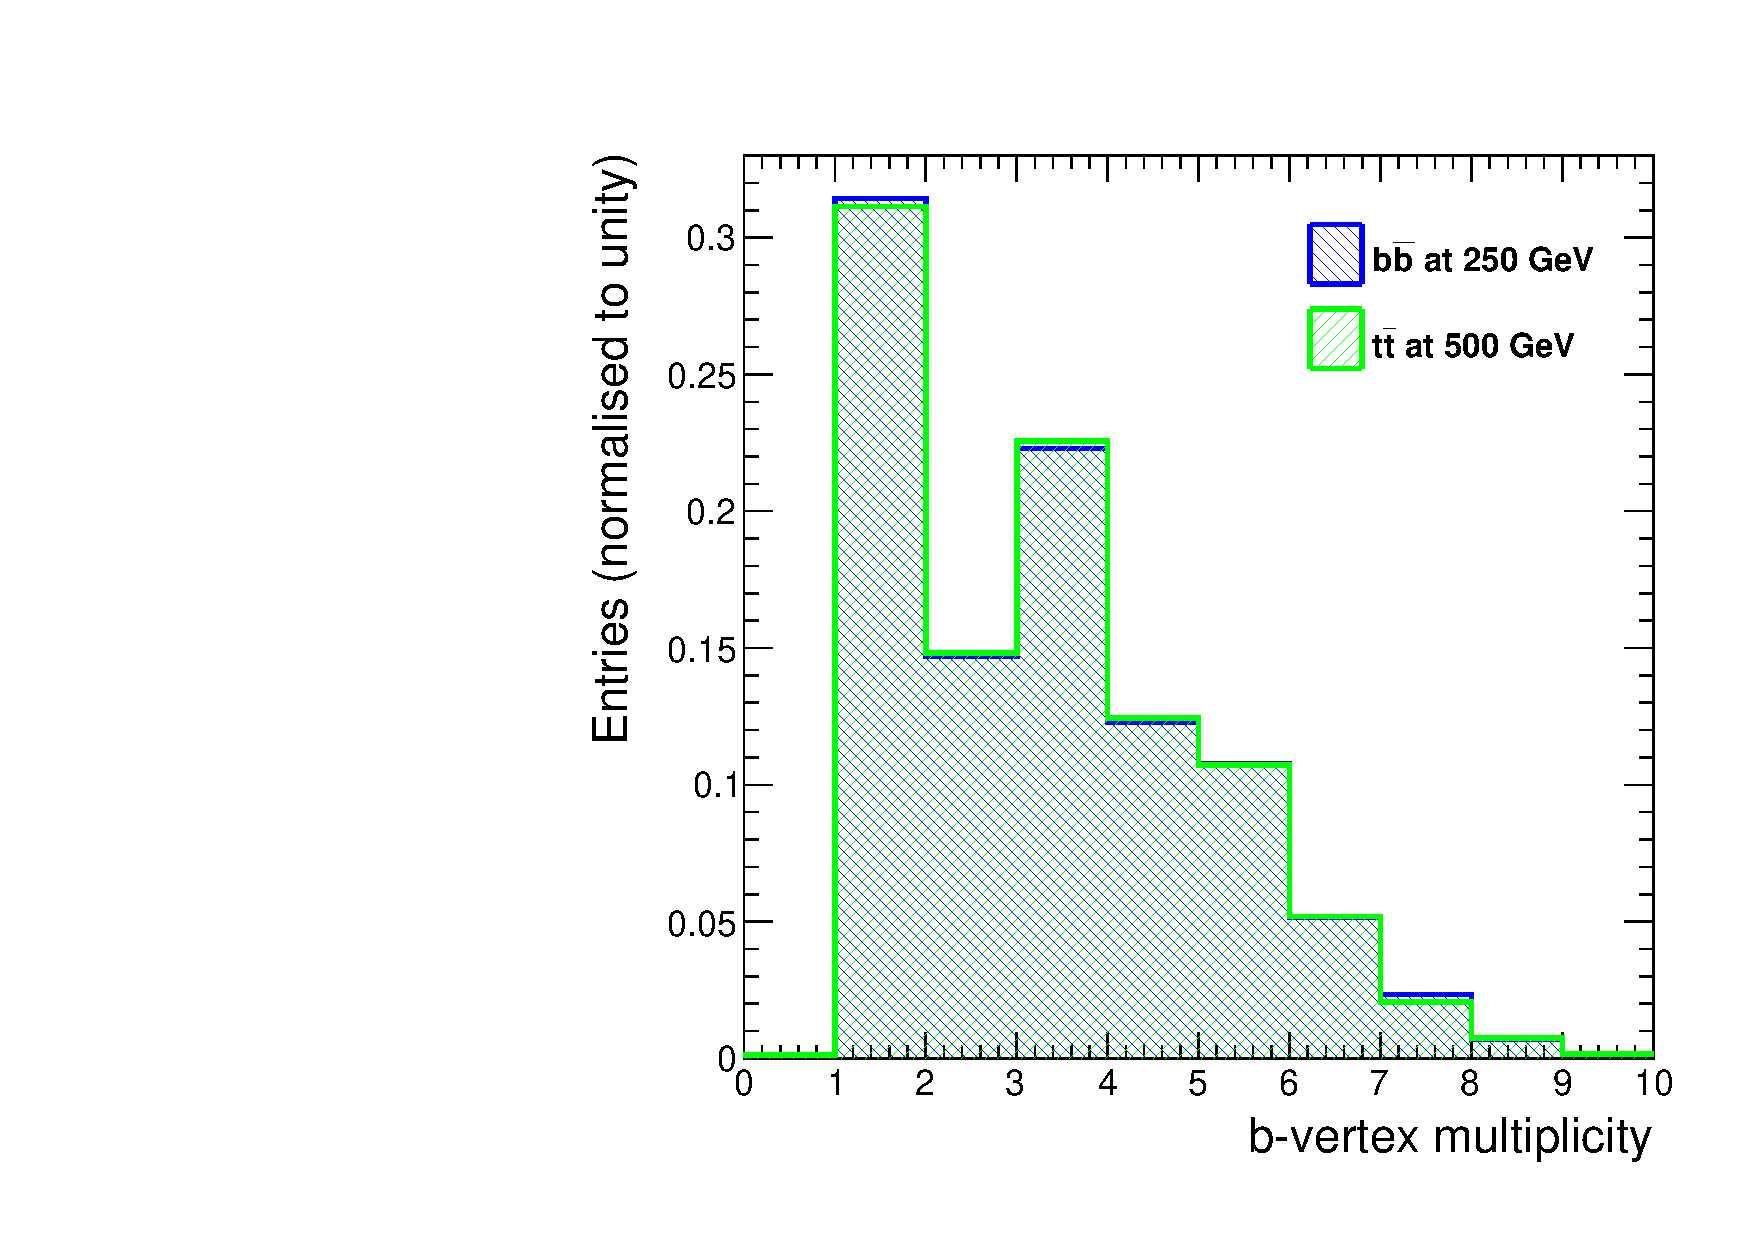
\includegraphics[width=0.95\textwidth]{ILD/plots/gen-b-vtx.pdf}
		\caption{\label{fig:GenVtx_a_3} }
	\end{subfigure}% 
	\begin{subfigure}{0.5\textwidth}
		\centering
		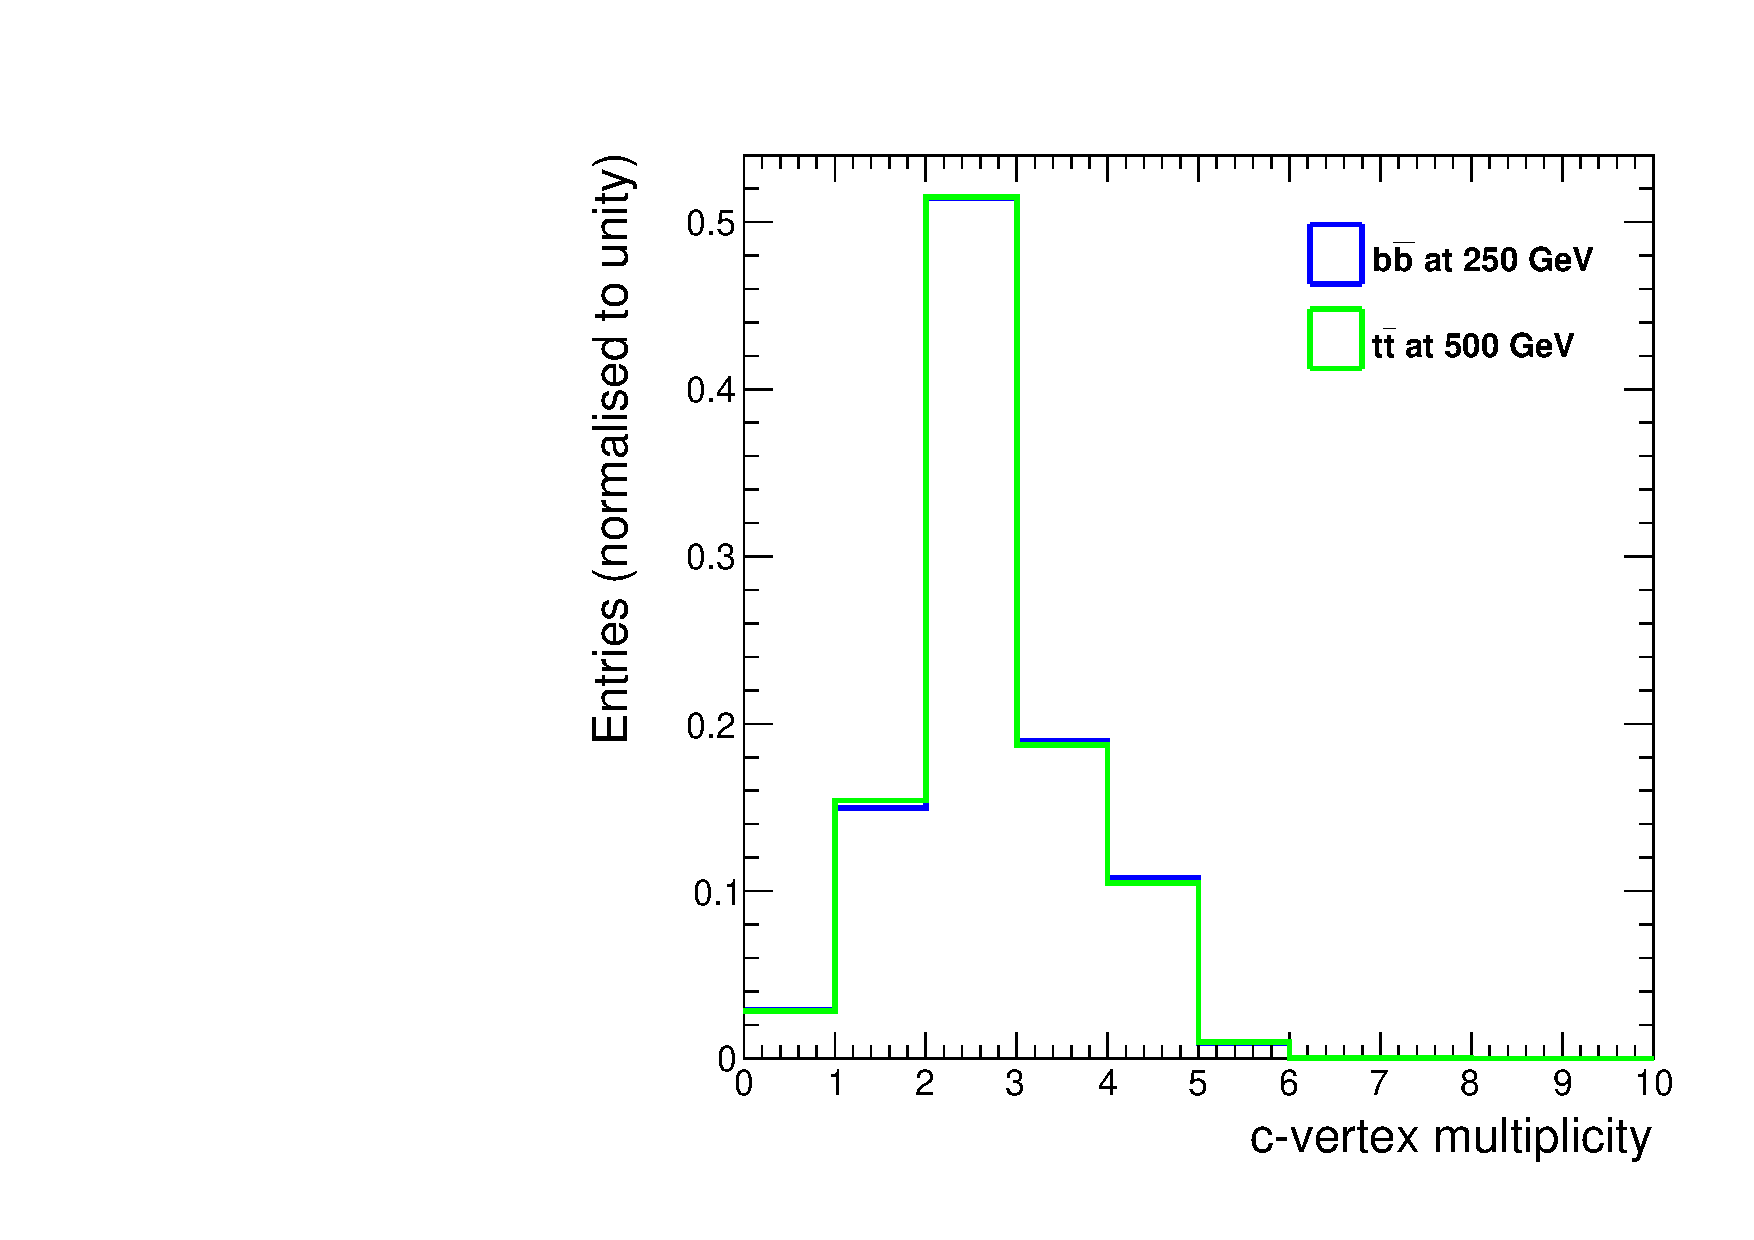
\includegraphics[width=0.95\textwidth]{ILD/plots/gen-c-vtx.pdf}
		\caption{\label{fig:GenVtx_b_3} }
	\end{subfigure}
	\caption{\sl Distributions of the b-vertex charge multiplicity~(a) and c-vertex charge multiplicity~(b). }
	\label{fig:GenVtx_3}
\end{figure}

%Generator distributions


%The b-hadrons can be identified by measuring the charged tracks, which have an offset from primary interaction point caused by the b-hadron lifetime.
%B*
The high-energy b-quarks can hadronize into excited states of the b-hadrons, which can decay into their ground state by emitting charged or neutral pion. 
The charged pion from the excited b-hadrons can distort the charge multiplicity distributions, leading to an incorrect comparison with the reconstructed vertices. Therefore, the TruthVertexFinder selects only ground state hadrons within a decay chain. 

The TruthVertexFinder finds vertices from b-hadron decays and subsequent c-hadron decay vertices. The distributions of generated b- and c-vertices are displayed in Fig.~\ref{fig:GenVtx_3}. 
The c-vertex multiplicity distribution is consistent with~\cite{bib:PDG}. 
One notices that about 31\% of the b-vertices and 13\% of the c-vertices decay into one generated prong, which poses a challenge to the vertexing algorithms. This problem will be addressed in Sec.~\ref{sec:MisVertices}.

\begin{figure}
	{\centering
		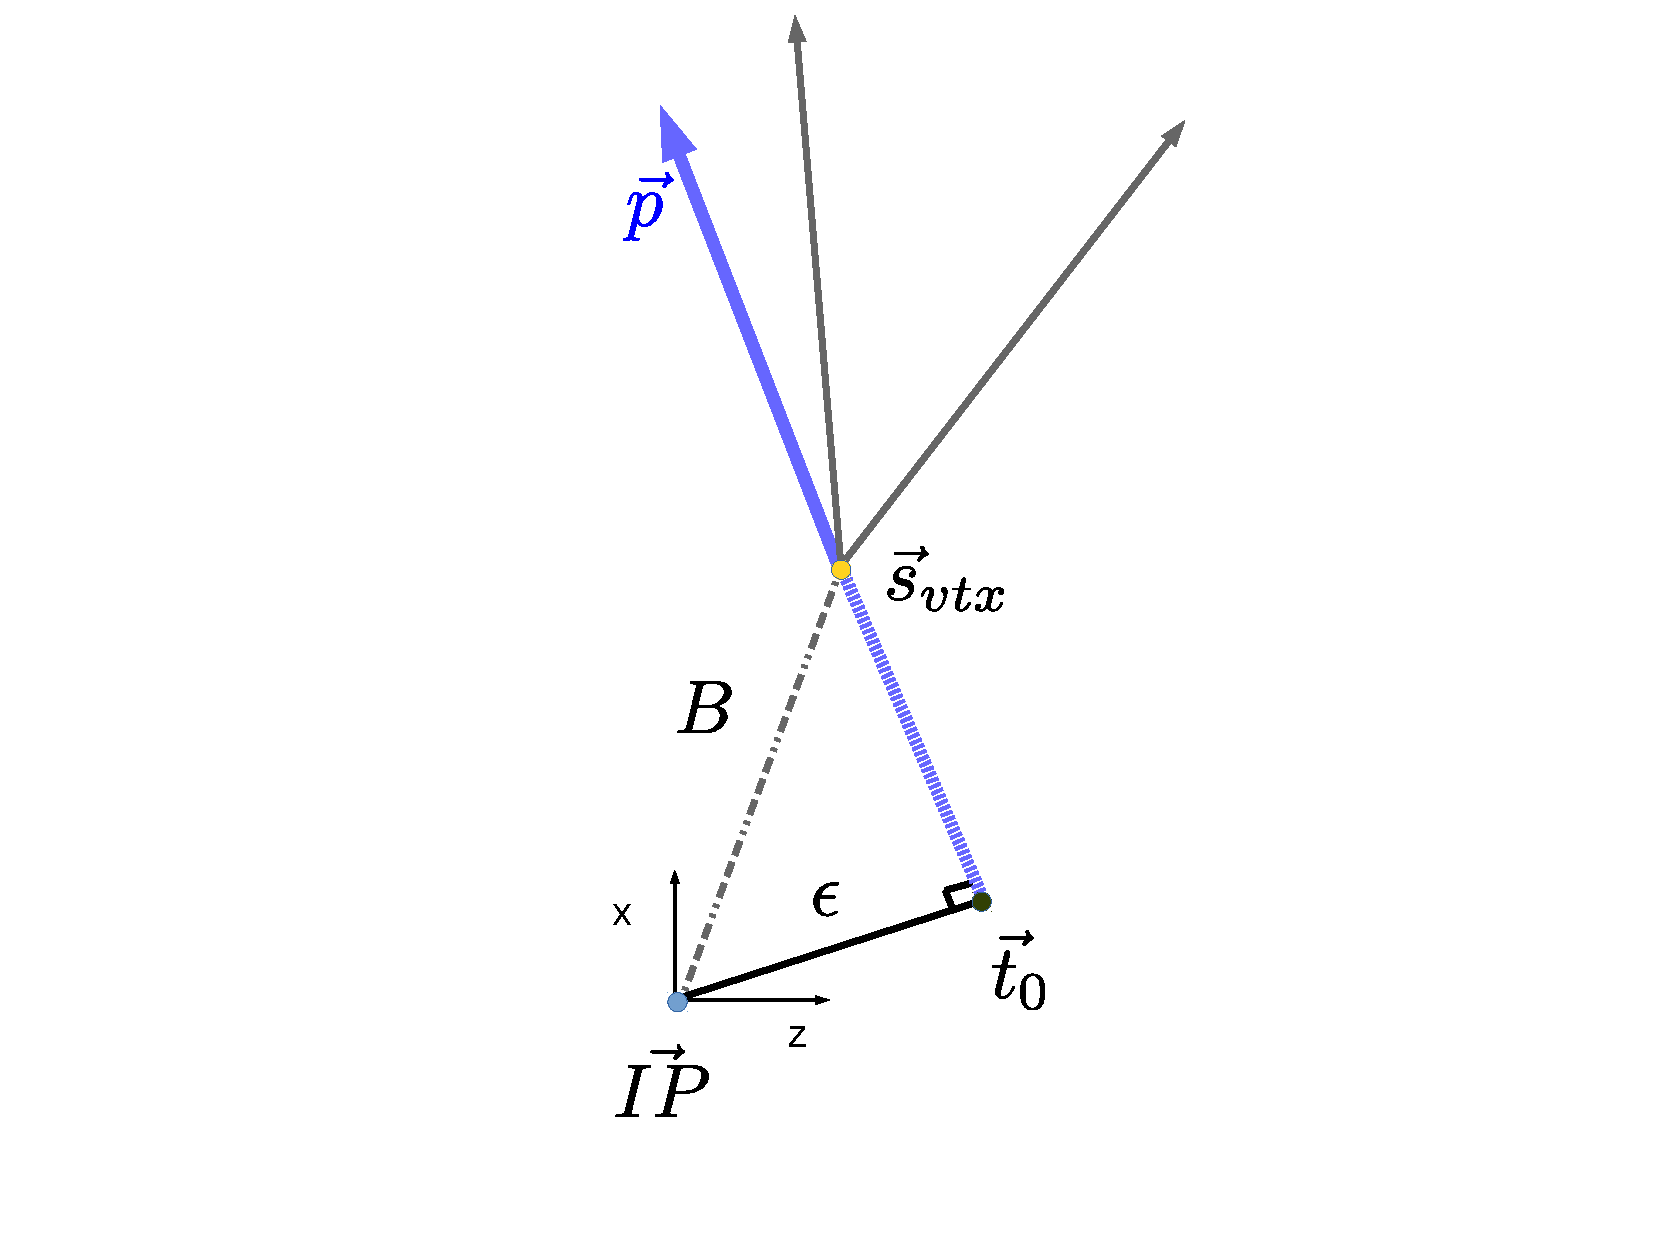
\includegraphics[width=0.75\textwidth]{ILD/plots/offset-graph.pdf}
		\caption{\sl Illustration of particle offset variable $\epsilon$, where $\vec{p}$ is a vector of a given particle momentum, $B$ is a flight distance of a b-hadron, $\vec{IP}$ is a primary vertex position, $\vec{t}_0$ is a point of the closest approach of a given particle. 
		}
		\label{fig:OffsetPic_3}
	}
\end{figure}

The particle offset or the impact parameter is the minimal distance between the particle trajectory and the interaction point, as illustrated in Fig.~\ref{fig:OffsetPic_3}.
This is the main observable used by the vertex reconstruction algorithms. 
The offset distributions of the generated b-vertex and c-vertex prongs are shown in Fig.~\ref{fig:GenVtxOffset_3}.
Majority of the generated prongs have large offsets above the ILD impact parameter resolution of 5\,$\mu$m. 
As can be seen from Fig.~\ref{fig:GenVtxOffset_3}, the c-vertex prong offsets are larger than b-vertex prong offsets, because of the additional distance traveled by c-hadron from the b-hadron decay point. 

\begin{figure}
\centering
\begin{subfigure}{0.5\textwidth}
    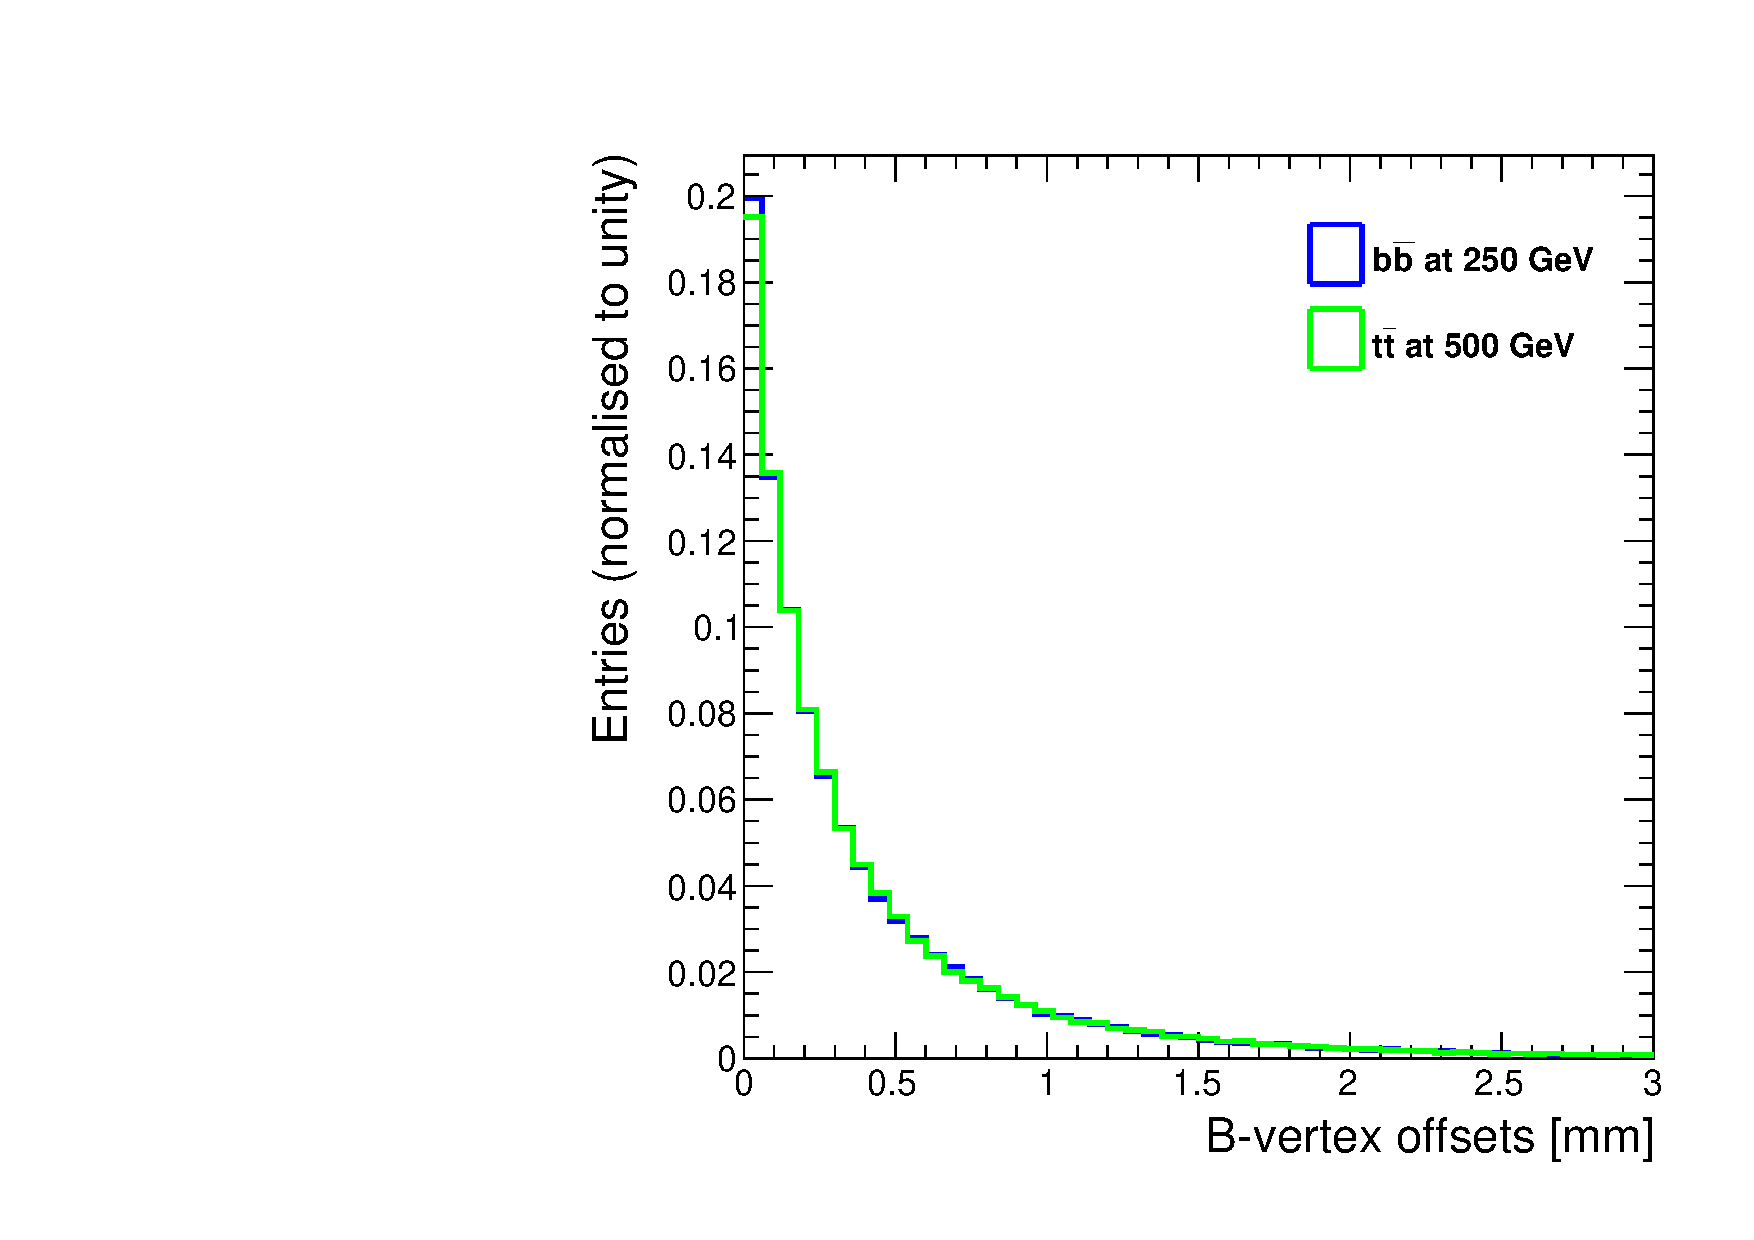
\includegraphics[width=0.95\textwidth]{ILD/plots/gen-bvtx-offsets.pdf}
\caption{\label{fig:GenVtxOffset_a_3} }
\end{subfigure}% 
  \begin{subfigure}{0.5\textwidth}
\centering
    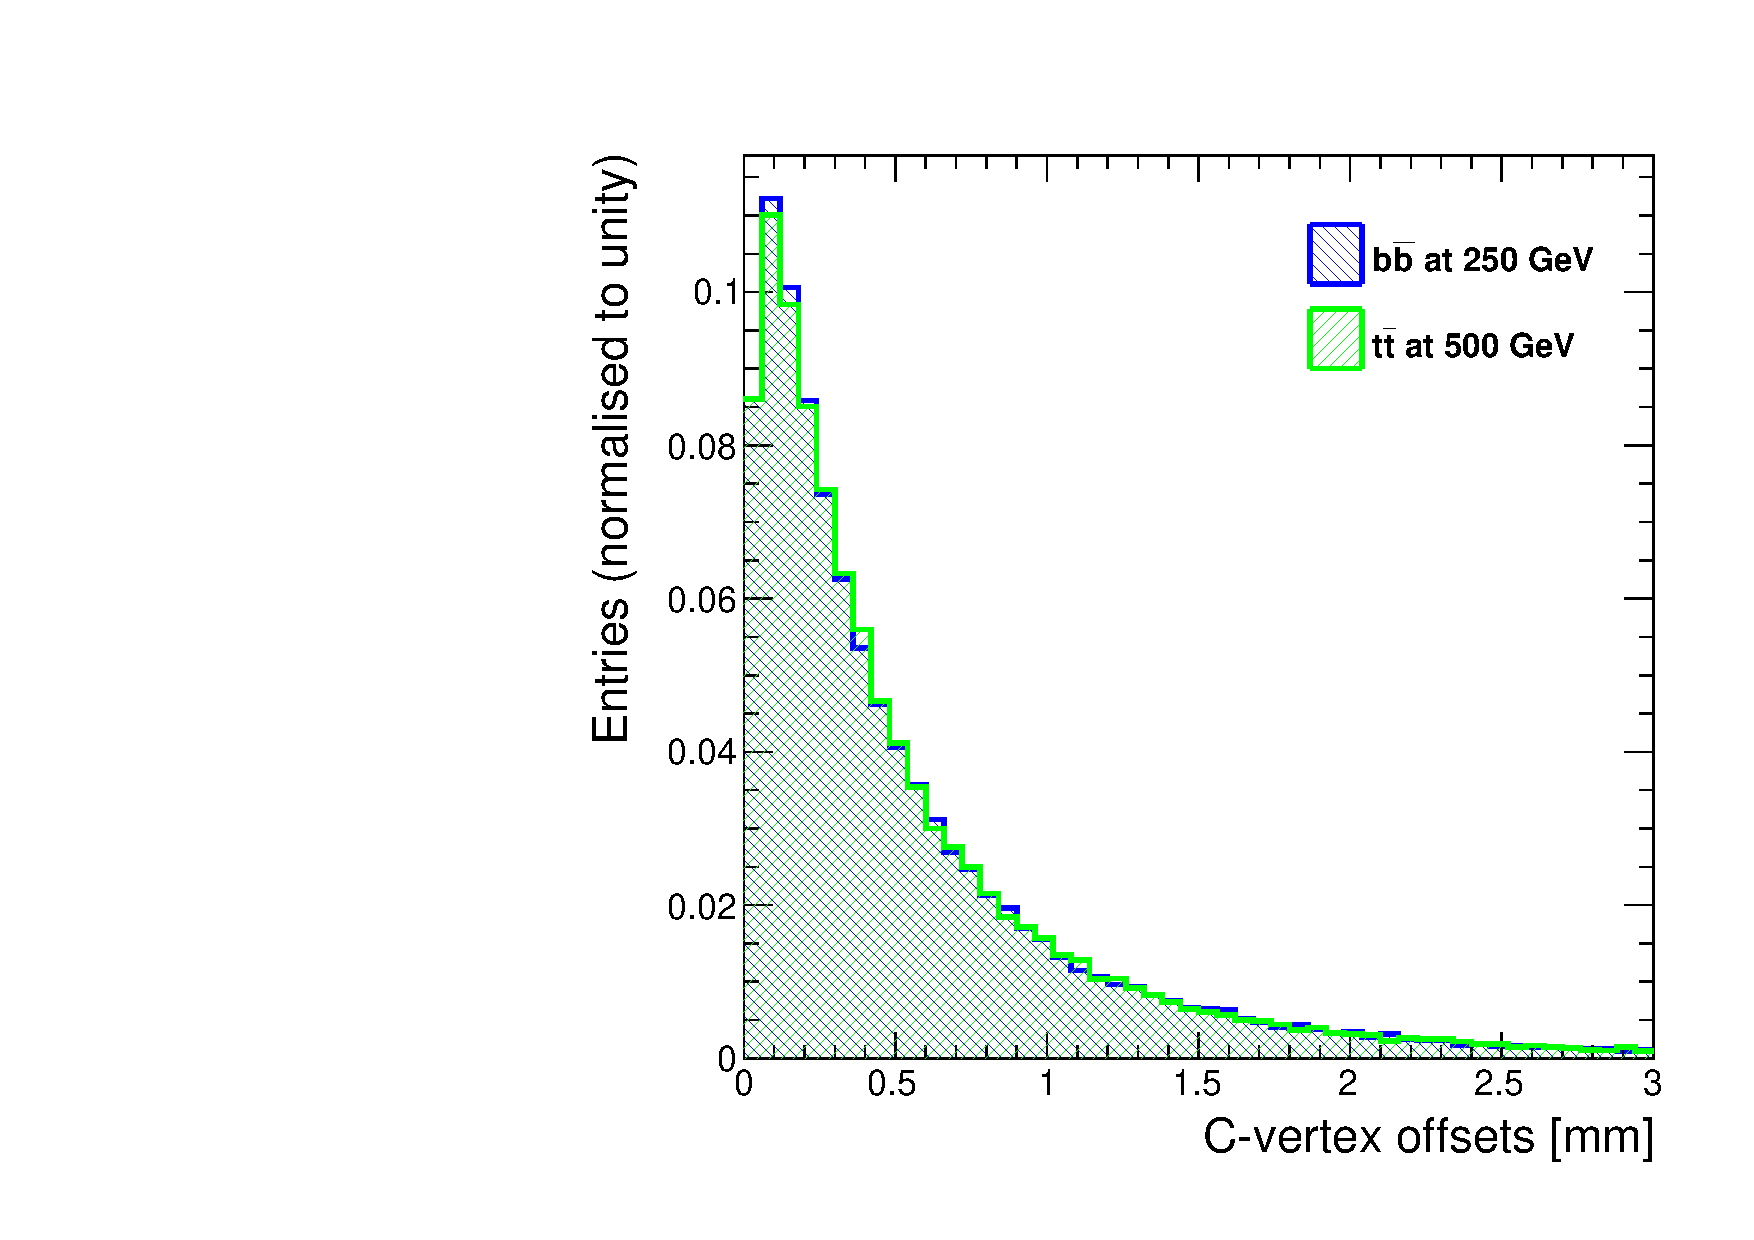
\includegraphics[width=0.95\textwidth]{ILD/plots/gen-cvtx-offsets.pdf}
\caption{\label{fig:GenVtxOffset_b_3} }
\end{subfigure}
    \caption{\sl Distributions of the b-vertex (a) and c-vertex prong offsets~(b). }
    \label{fig:GenVtxOffset_3}
\end{figure}

The distributions of the total B-hadron charge multiplicity and the b-jet multiplicity are displayed in Fig.~\ref{fig:GenHadronParams_3}. The mean b-jet multiplicity is almost three times higher than the mean B-hadron multiplicity, which makes the vertex reconstruction a non trivial task. 
The imbalance between the odd and even number of multiplicities shown in Fig.~\ref{fig:GenHadronParams_a_3} is caused by the presence of the \Bzs\ hadronization modes.

Regarding the similarity of the distributions for two processes shown in Figures~\ref{fig:GenVtx_3}, \ref{fig:GenHadronParams_3} and \ref{fig:GenVtxOffset_3}, the performance of a vertexing algorithm should be identical for the same energy and the direction of the b-hadron decays.


\begin{figure}
\centering
\begin{subfigure}{0.5\textwidth}
    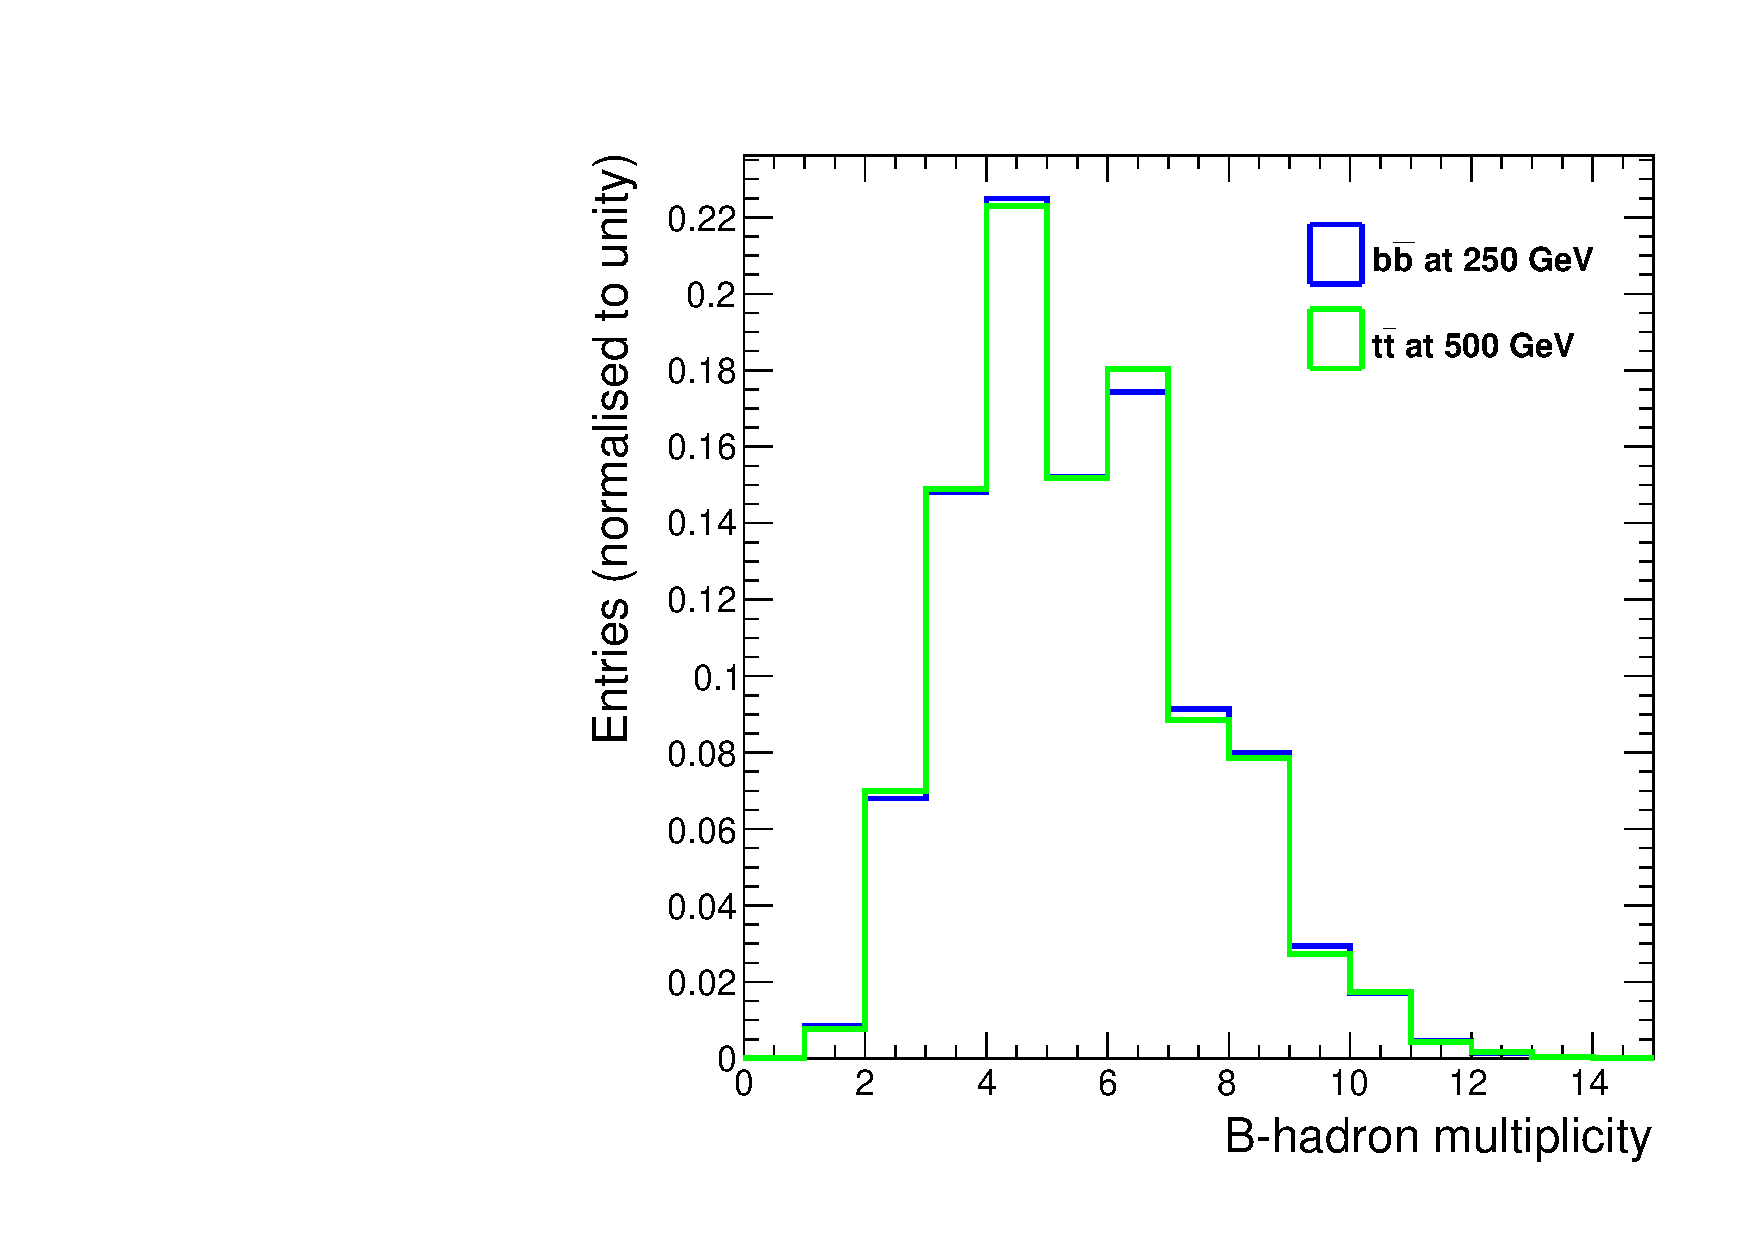
\includegraphics[width=0.95\textwidth]{ILD/plots/gen-hadron-multiplicity.pdf}
\caption{\label{fig:GenHadronParams_a_3} }
\end{subfigure}% 
  \begin{subfigure}{0.5\textwidth}
\centering
    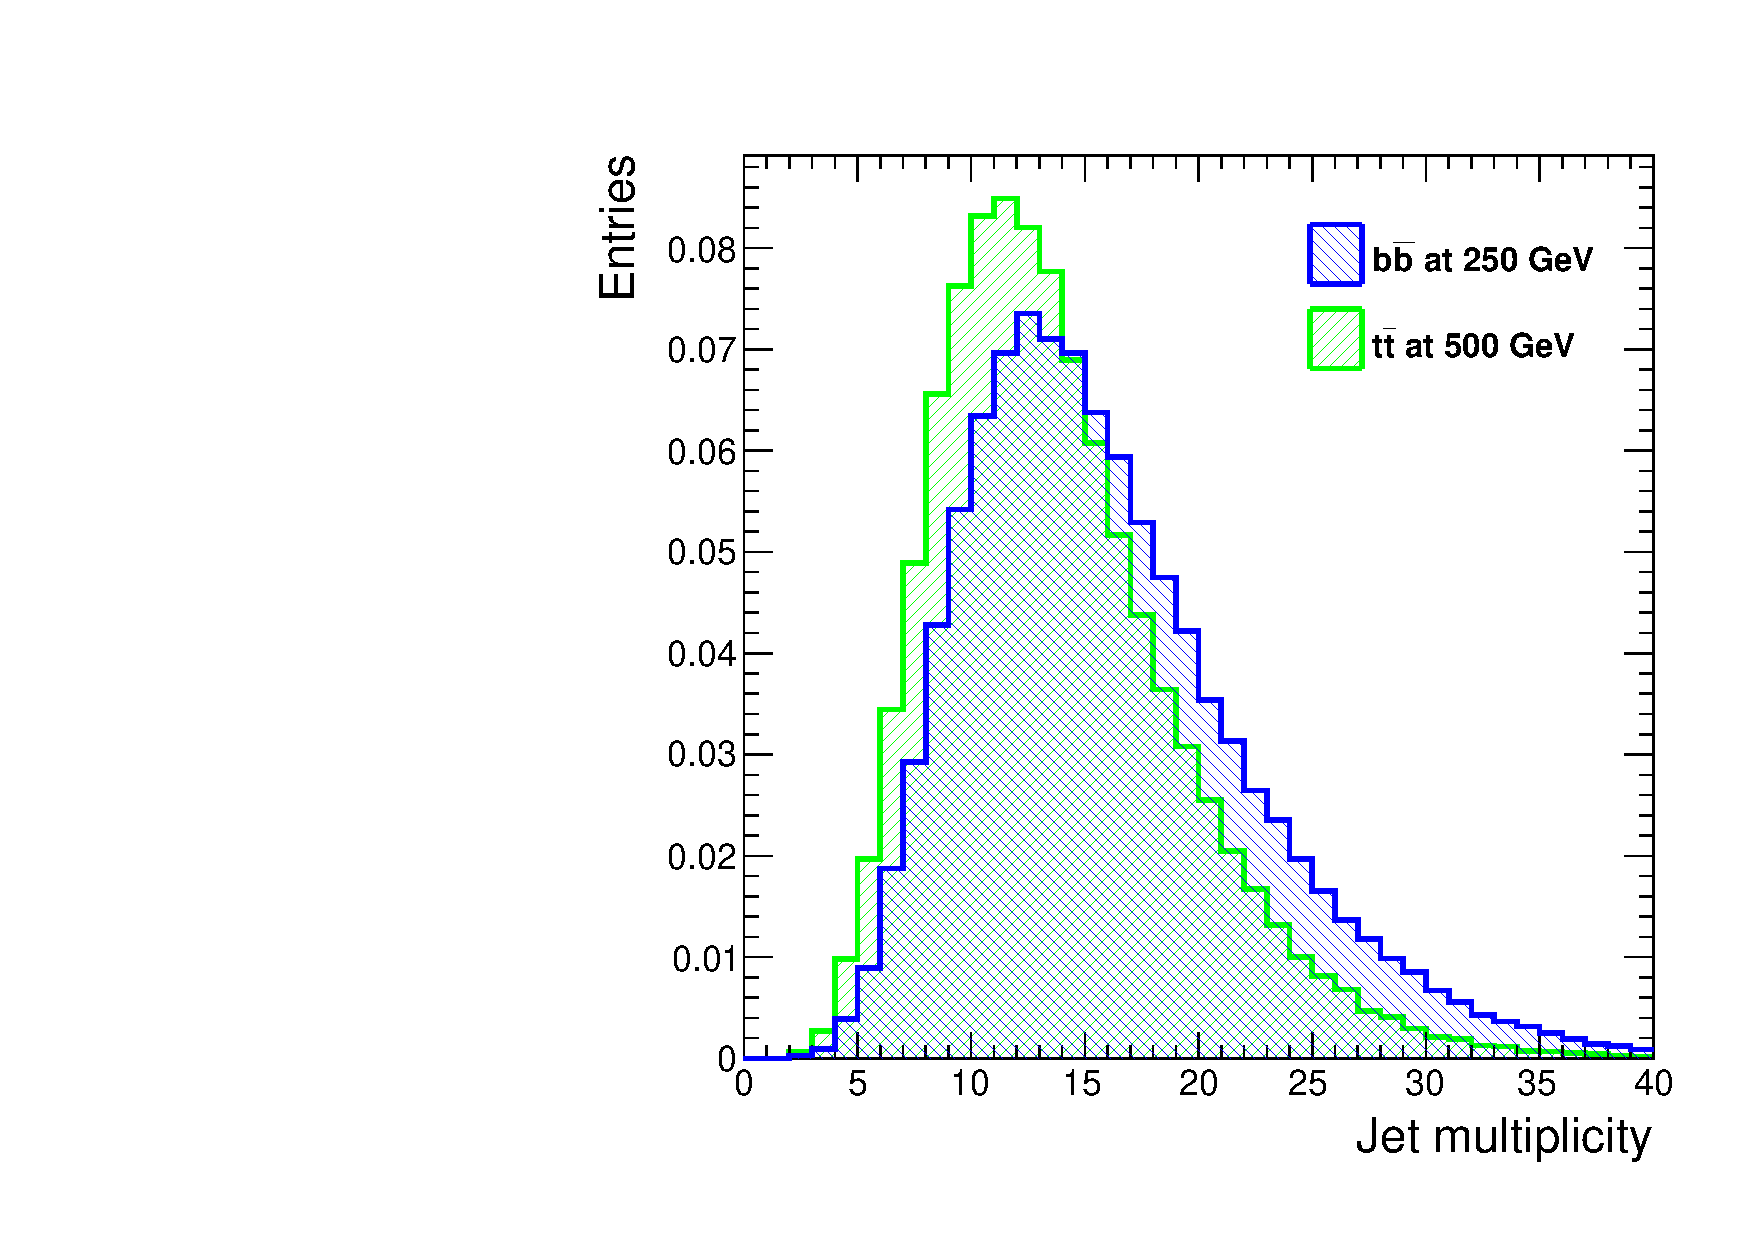
\includegraphics[width=0.95\textwidth]{ILD/plots/jet-multi.pdf}
\caption{\label{fig:GenHadronParams_b_3} }
\end{subfigure}
    \caption{\sl Left: Distribution of the b-hadron charge multiplicity. The odd multiplicities correspond to the charged hadrons and the even multiplicities correspond to the neutral hadron decays. Right: Distribution of the reconsructed b-jet multiplicities for two processes. }
    \label{fig:GenHadronParams_3}
\end{figure}


%The design of the ILD vertex detector is optimized to have the best offset resolution 

%%%%%%%%%%%%%%%%%%%%%%%%%%%%%%%%%%%%%%%%%%%%%%%%%%%%%%%%%
%%%%%%%%%%%%%%%%%%%%%%%%%%%%%%%%%%%%%%%%%%%%%%%%%%%%%%%%%
%%%%%%%%%%%%%%%%%%%%%%%%%%%%%%%%%%%%%%%%%%%%%%%%%%%%%%%%%

\subsection{Standard vertex reconstruction in the ILD}
The LCFI+ package finds the secondary and tertiary vertices and tags the b- and c-jets using the charged particles among the Particle Flow objects.
It has several stages of the vertex reconstruction and flavor-tagging, which are implemented in the following algorithms:
\begin{itemize}
\item PrimaryVertexFinder finds the position of the primary interaction point and the corresponding charged particles;
\item BuildUpVertex forms the reconstructed vertex candidates, which can have two or more associated charged particles, referred in the text as reconstructed prongs;
\item JetVertexRefiner finds vertices with only one prong using the reconstructed vertex candidates and it organizes the vertex candidates into maximum two reconstructed vertices per jet.
\item FlavorTag algorithm calculates b-tag and c-tag values for a jet, using the finalized jet vertices from the JetVertexRefiner. The b-tag and c-tag values are the measure of b- and c-likeness of a jet, respectively, both observables have values from 0 to 1. Performance of the flavor-tagging algorithm is shown in Fig.~\ref{fig:LCFIplus_3}.
\end{itemize}

\begin{figure}
	{\centering
		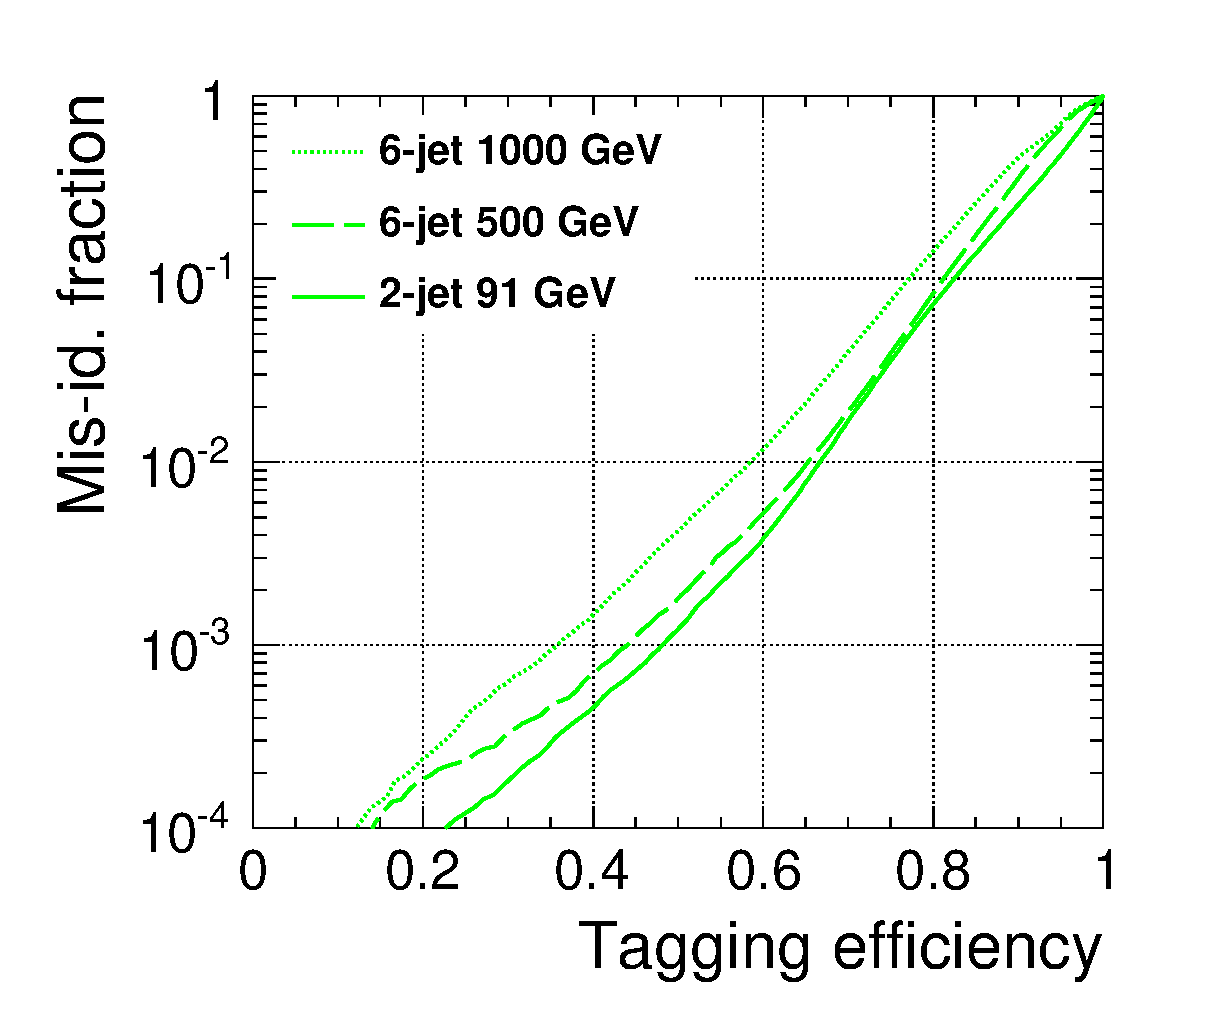
\includegraphics[width=0.45\textwidth]{ILD/graphics/btag-cbg.eps}
		\caption{\sl The tagging efficiency is shown for b-jets with the mis-identification	fraction evaluated using c-jets. Solid lines correspond to the case of 2-jet events at $\sqrt{s} = 91$\,GeV. Dashed lines correspond to the case of 6-jet events at	$\sqrt{s} = 500$\,GeV. Dotted lines correspond to the case of 6-jet events at $\sqrt{s} = 1000$\,GeV~\cite{bib:LCFI}.
		}
		\label{fig:LCFIplus_3}
	}
\end{figure}
In this section, only the standard reconstruction chain is used to study the b-quark charge measurement. 


%\subsubsection{Baseline quark charge reconstruction}
The b-quark charge is computed as a sum of the reconstructed particles charges, associated to the reconstructed vertices, which belong to a given jet. 
Therefore, the vertexing algorithm should correctly associate all secondary or tertiary vertex particles to have a correct b-quark charge measurement. 
The correctly reconstructed b-quark charge should have the same  charge as the generated b-hadron. 
%Regarding the b-hadron multiplicity, shown in Fig.~\ref{fig:GenHadronParams_a_3}, and the b-jet multiplicity in Fig.~\ref{fig:GenHadronParams_b_3} this task is not trivial. 

%%%%%%%%%%%%%%%%%%%%%%%%%%%%%%%%%%%%%%%%%%%%%%%%%%%%
%%%%%%%%%%%%%%%%%%%%%%%%%%%%%%%%%%%%%%%%%%%%%%%%%%%%
%%%%%%%%%%%%%%%%%%%%%%%%%%%%%%%%%%%%%%%%%%%%%%%%%%%%
\subsubsection{B-quark charge purity: State of the art}
The charge purity $P_B$ is defined as the number of correctly reconstructed b-quark charges $N_{correct}$ divided by the total number of jets $N_{total}$:
\begin{equation}
	\label{formula:Purity_3}
	P_B = \frac{N_{correct}}{N_{total}}.
\end{equation} 
The previous studies carried out for the fully hadronic $t\bar{t}$ decays~\cite{Amjad:2014tha} have shown that the total b-quark charge purity $P_B$ is about 60\%.
The total b-quark charge for the considered $b\bar{b}$ process  is $P_B(b\bar{b}) = 66\%$ and for semileptonic decay of the  $t\bar{t}$ pair is $P_B(t\bar{t}) = 64\%$. 
The small difference between these values is caused mostly by the difference in the generated momentum  distributions displayed in Fig.~\ref{fig:GenHadronMomentum_3} and by the difference in the jets environments.

Using the output of the TruthVertexFinder, one compares the generated vertices with the corresponding reconstructed vertices, detected by the LCFI+ algorithms. 
Figure~\ref{fig:Table_3} shows the comparison of the number of the generated prongs $N_{gen}$ with the number of the reconstructed prongs $N_{rec}$ on the jet-per-jet basis. 
The row with $N_{rec} = 0$ are the jets, which have no associated reconstructed vertices, will cause the efficiency decrease in the b-quark charge measurement, however, they have no influence on the method purity.
The jets with reconstructed vertices have the following statistics:
\begin{itemize}
\item Only 49\% of these jets are perfectly reconstructed and have $N_{rec}=N_{gen}$;
\item The 46\% of the jets have lost one or more prongs from the reconstructed vertices having $N_{rec}<N_{gen}$;
\item The rest 5\% are the jets with vertices, contaminated by particles with non b-hadron origin and have $N_{rec}>N_{gen}$.
\end{itemize}

\begin{figure}
{\centering
    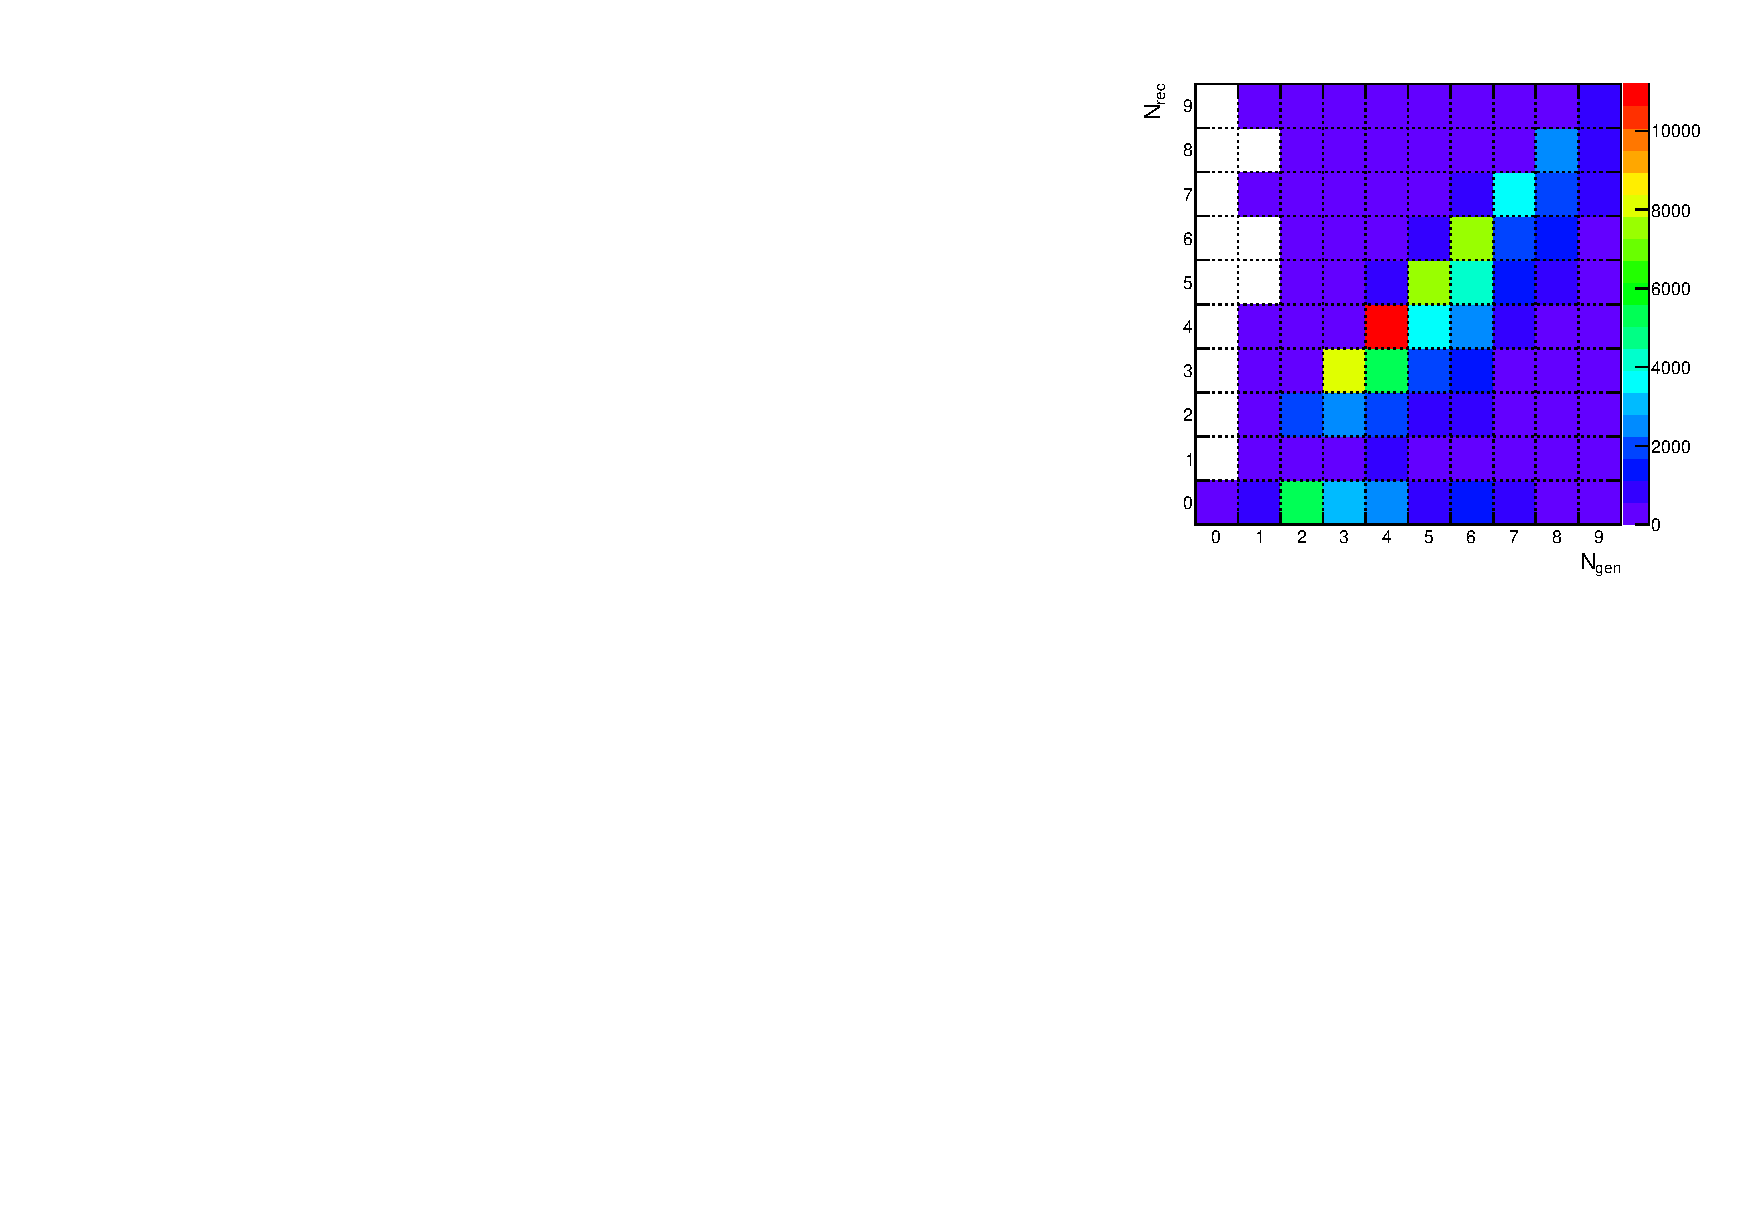
\includegraphics[width=0.55\textwidth]{ILD/plots/rec-gen-table.pdf}
    \caption{\sl Comparison of the number of reconstructed tracks $N_{gen}$ to the number of generated tracks $N_{rec}$ for a given b-jet. The number of entries is color-coded for each cell. The diagonal has 49\% of all entries and it contains the jets, which have the correctly reconstructed vertices. The b-jets below diagonal have vertices with one or more particles missed by reconstruction. The row $N_{rec} = 0$ corresponds to the b-jets with no reconstructed vertices. %Right: Same comparison, but after a cut on the b-tag$> 0.8$ and a cut on the b-hadron momentum more than 20\,GeV. The diagonal contains 55\% of the jets after the cuts.
    }
    \label{fig:Table_3}
  }
\end{figure}

The jets with $N_{rec}=N_{gen}$ have the charge purity of more than 97\%, while all other jets have an almost random reconstructed b-quark charge with the corresponding charge purity about 35\%.
The fraction of entries below the diagonal in Fig.~\ref{fig:Table_3} is small, comparing to the fraction of events above the diagonal. 
Hence, the purity reduction is mainly caused by the jets, which have lost the prongs from their reconstructed vertices. 
%The application of cuts, for example on jet b-tag$>0.8$ and reconstructed b-hadron momentum $|p_{had}| > 20$\,GeV, increases the fraction of correctly reconstructed jets up to 55\%, however with an efficiency penalty of 17\%.
%The cuts on the b-tag value are necessary to reject background processes and will be adjusted to archieve the best background suppression. 


Therefore, there is a possibility to develop a recovery algorithm, which can add the missing prongs to the reconstructed vertices.
%, with a slight increase of the number of jets with contaminated vertices. 
But first, one needs to study the reasons behind the missing prongs and analyze the possibility to recover them. 

%%%%%%%%%%%%%%%%%%%%%%%%%%%%%%%%%%%%%%%%%%%%%%%%%%%%
%%%%%%%%%%%%%%%%%%%%%%%%%%%%%%%%%%%%%%%%%%%%%%%%%%%%
%%%%%%%%%%%%%%%%%%%%%%%%%%%%%%%%%%%%%%%%%%%%%%%%%%%%
\subsubsection{Missing vertices}
\label{sec:MisVertices}
The vertex reconstruction algorithm may fail if the generated b-hadron properties, like number of generated prongs, b-hadron momentum or polar angle, are in the poor acceptance of the detector. 
The non-reconstructed vertices contain approximately 22\% of all generated b-hadron prongs. 
The b-hadron vertices with generated low momentum prongs or low offset prongs have higher chances to be missed by the reconstruction algorithms. 
The distributions of the average prong offset and momentum for reconstructed vertices and missed vertices are shown in Fig.~\ref{fig:RecMissedParams_3}. 
One concludes, that the reconstruction algorithms start to lose their efficiency at below 4\,GeV average prong momentum and below 0.5\,mm average prong offset. 


The polar angle distributions of the missing vertices is displayed in Fig.~\ref{fig:MissedCos_3}. 
One summarizes the reasons for missing vertices as following: 
\begin{itemize}
\item Neutral decay vertex - the vertex cannot be reconstructed if it has no generated prongs;
\item Low energy of the generated b-hadron causes a short flight distance, small offsets or low momentum of the generated prongs, which makes it difficult to separate out the b-hadron prongs from the other particles in a b-jet;
\item A one prong decay vertex can be lost if there was no other vertices reconstructed in a given b-jet;
\item Most of the b-hadrons, produced in the forward region, or outside the barrel VXD acceptance $|\cos\theta_{vtx}| > 0.95$, are not reconstructed, which is due to a low precision on the impact parameters of the reconstructed prongs. 
\end{itemize}

\begin{figure}
	\centering
	\begin{subfigure}{0.5\textwidth}
		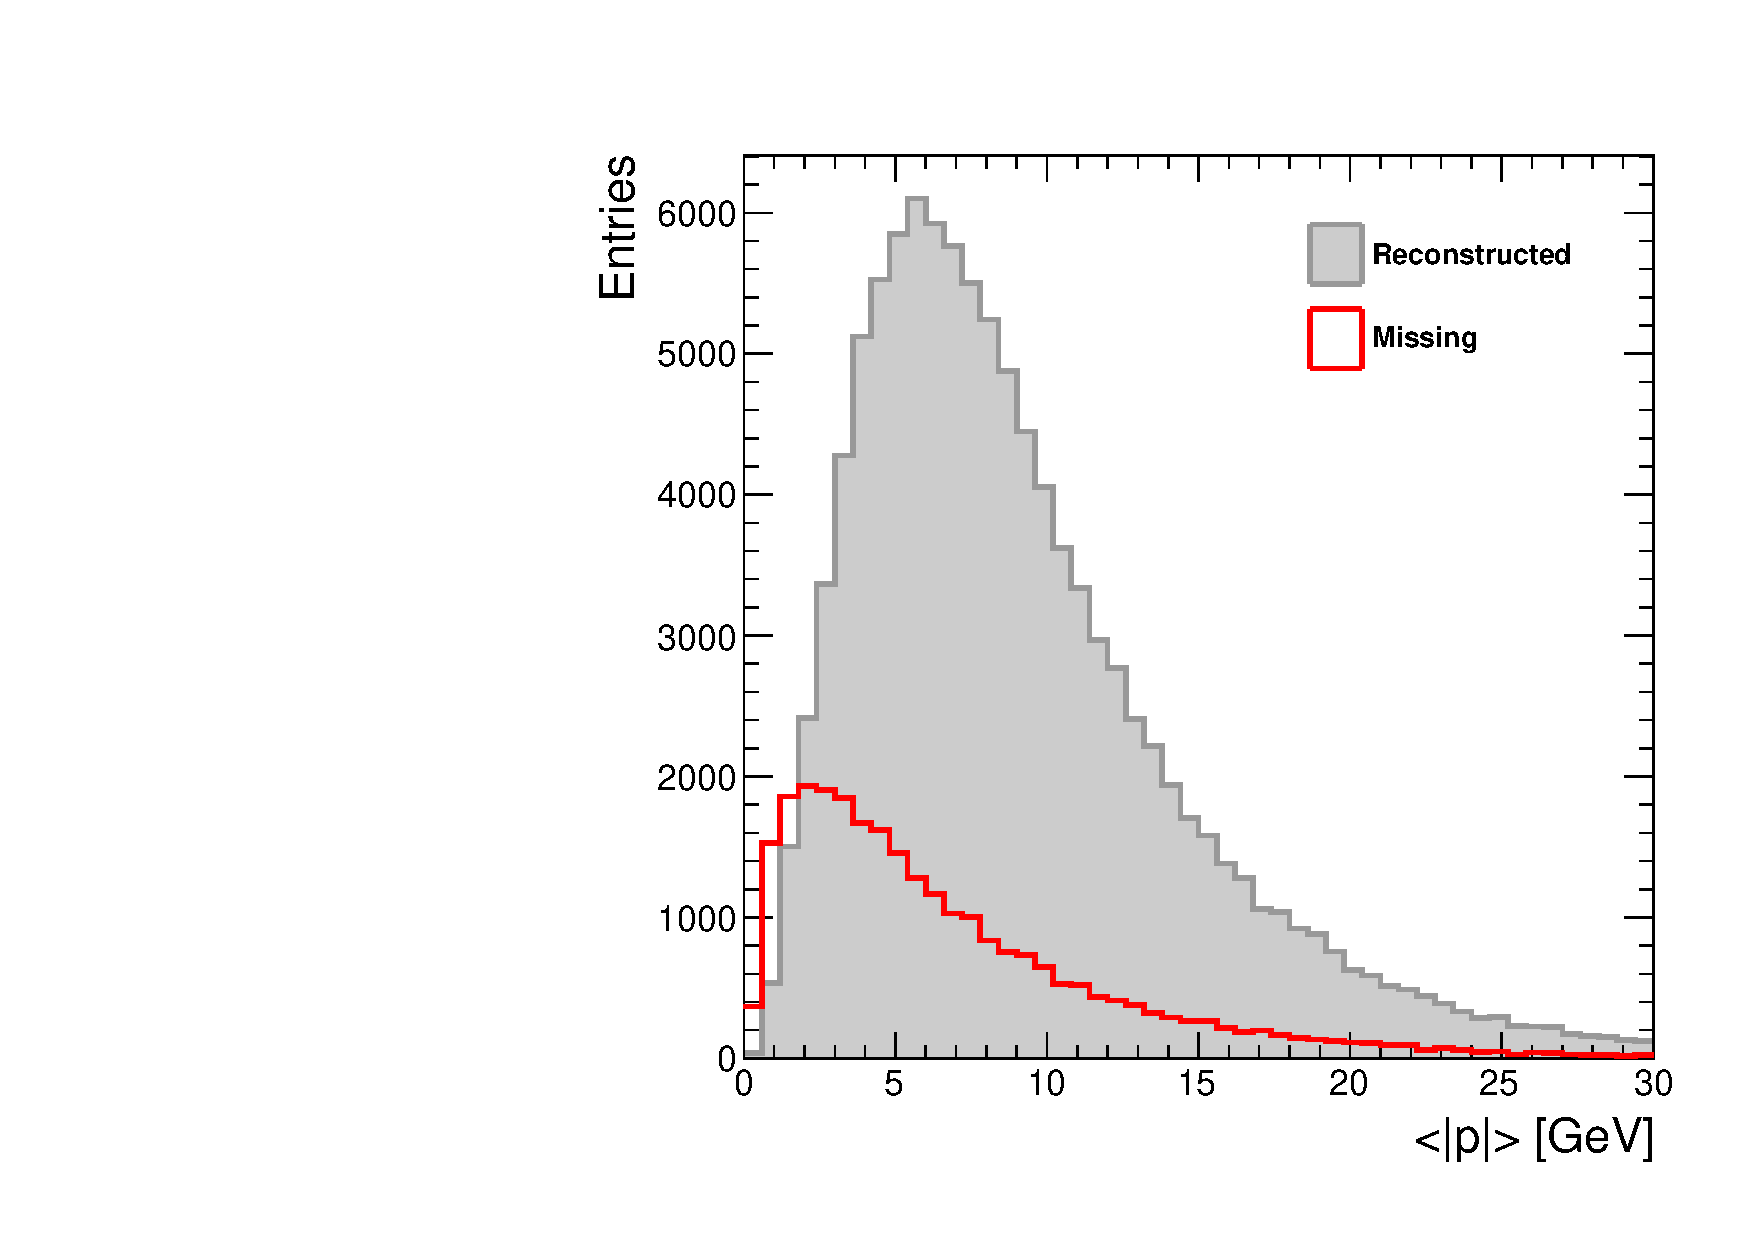
\includegraphics[width=0.95\textwidth]{ILD/plots/rec-missed-p-vtx.pdf}
		\caption{\label{fig:RecMissedParams_a_3} }
	\end{subfigure}% 
	\begin{subfigure}{0.5\textwidth}
		\centering
		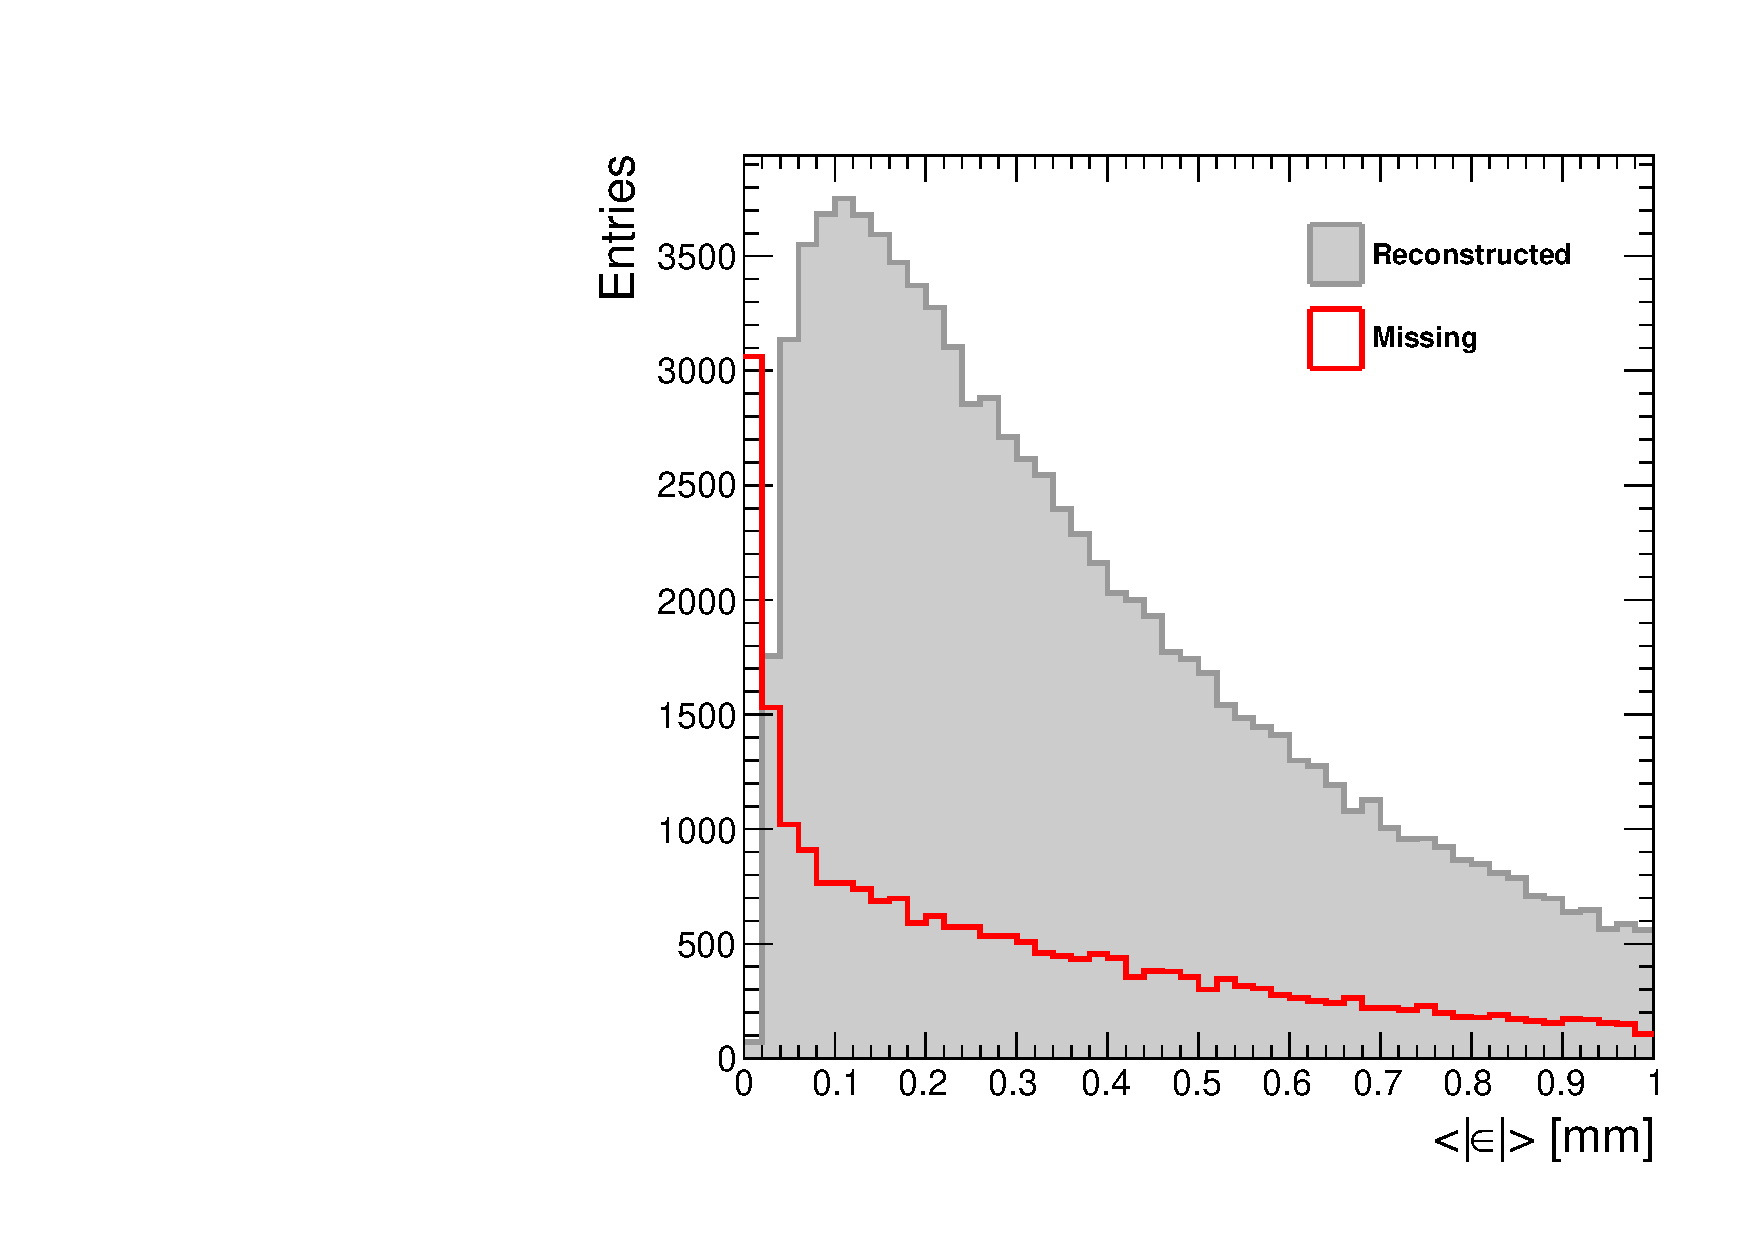
\includegraphics[width=0.95\textwidth]{ILD/plots/rec-missed-s-vtx.pdf}
		\caption{\label{fig:RecMissedParams_b_3} }
	\end{subfigure}
	\caption{\sl Distributions of the average prong momentum~(a) and offset (b) of the missed and reconstructed vertices. }
	\label{fig:RecMissedParams_3}
\end{figure}

\begin{figure}
	{\centering
		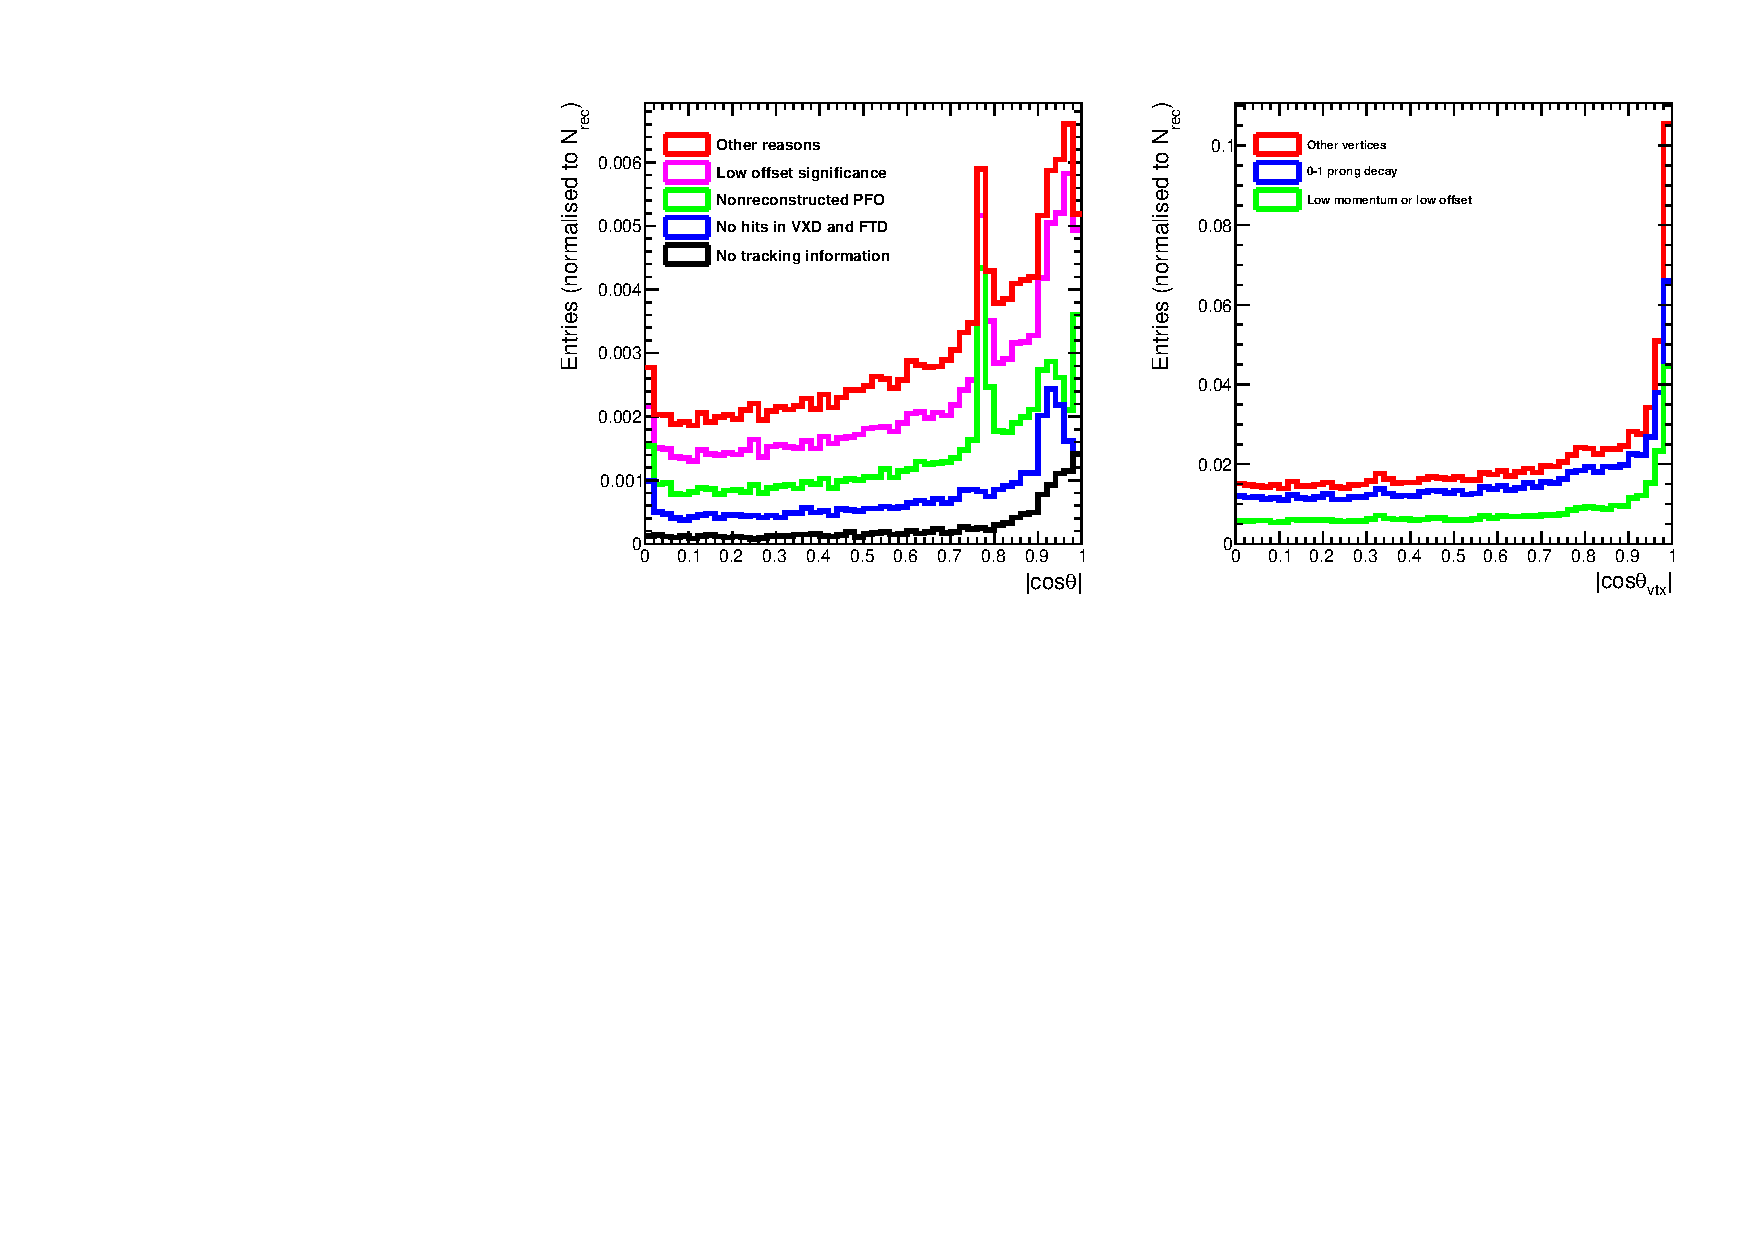
\includegraphics[clip, trim=10.cm 0cm 0.cm 0cm, width=0.55\textwidth]{ILD/plots/missed-cos-vtx.pdf}
		\caption{\sl Polar angle distribution of the missed vertices subdivided into different categories. This is a stacked histogram. The low momentum or low offset category are the missing vertices, which have the average prong momentum below  4\,GeV or below 0.5\,mm average prong offset.
		}
		\label{fig:MissedCos_3}
	}
\end{figure}
%An attempt was made to reduce the vertexing inefficiency in the forward region

The missing vertices are difficult to recover, however they have essentially no impact on the b-quark charge purity, therefore the further studies are focused on the missing prongs of the reconstructed vertices.
%%%%%%%%%%%%%%%%%%%%%%%%%%%%%%%%%%%%%%%%%%%%%%%%%%%%
%%%%%%%%%%%%%%%%%%%%%%%%%%%%%%%%%%%%%%%%%%%%%%%%%%%%
%%%%%%%%%%%%%%%%%%%%%%%%%%%%%%%%%%%%%%%%%%%%%%%%%%%%
\subsubsection{Missing prongs from the reconstructed vertices}
\label{sec:MissingProngs}
%The quality of the vertex reconstruction strongly depends on all reconstruction algorithms as well as on various geometry aspects of the ILD experiment. 

%Using TruthVertexFinder information and truth links to the reconstructed particles, one can find, that the 
The missing reconstructed prongs are approximately 10.4\% of the total generated prongs for the standard vertex reconstruction. 
The reasons for the missing prongs can be summarized as follows:
\begin{itemize}
\item No tracking information - the MarlinTrk algorithms fails to reconstruct the track. This category is tiny - only 0.93\% of the generated prongs;
\item No associated hits in the VXD or FTD - the track segment from the Vertex Detector or Forward Tracking Disks was not connected to the long TPC track segment. These reconstructed particles have large uncertainties on the impact parameters, which makes them not suitable for vertexing algorithms. They constitute 2.\% of the generated prongs;
\item No reconstructed PFO - the PandoraPFA fails to create the PFO from a reconstructed track. These tracks are discarded by the LCFI+ algorithms - 3.2\%  of the generated prongs;
\item Low generated momentum or offset  - the reconstructed particle was produced with impact parameters below the detector resolution - 3.1\%  of the generated prongs;
\item Other reasons connected to vertex fitting problems - 1.7\% of the generated prongs.
\end{itemize}



\begin{figure}
\centering
\begin{subfigure}{0.5\textwidth}
    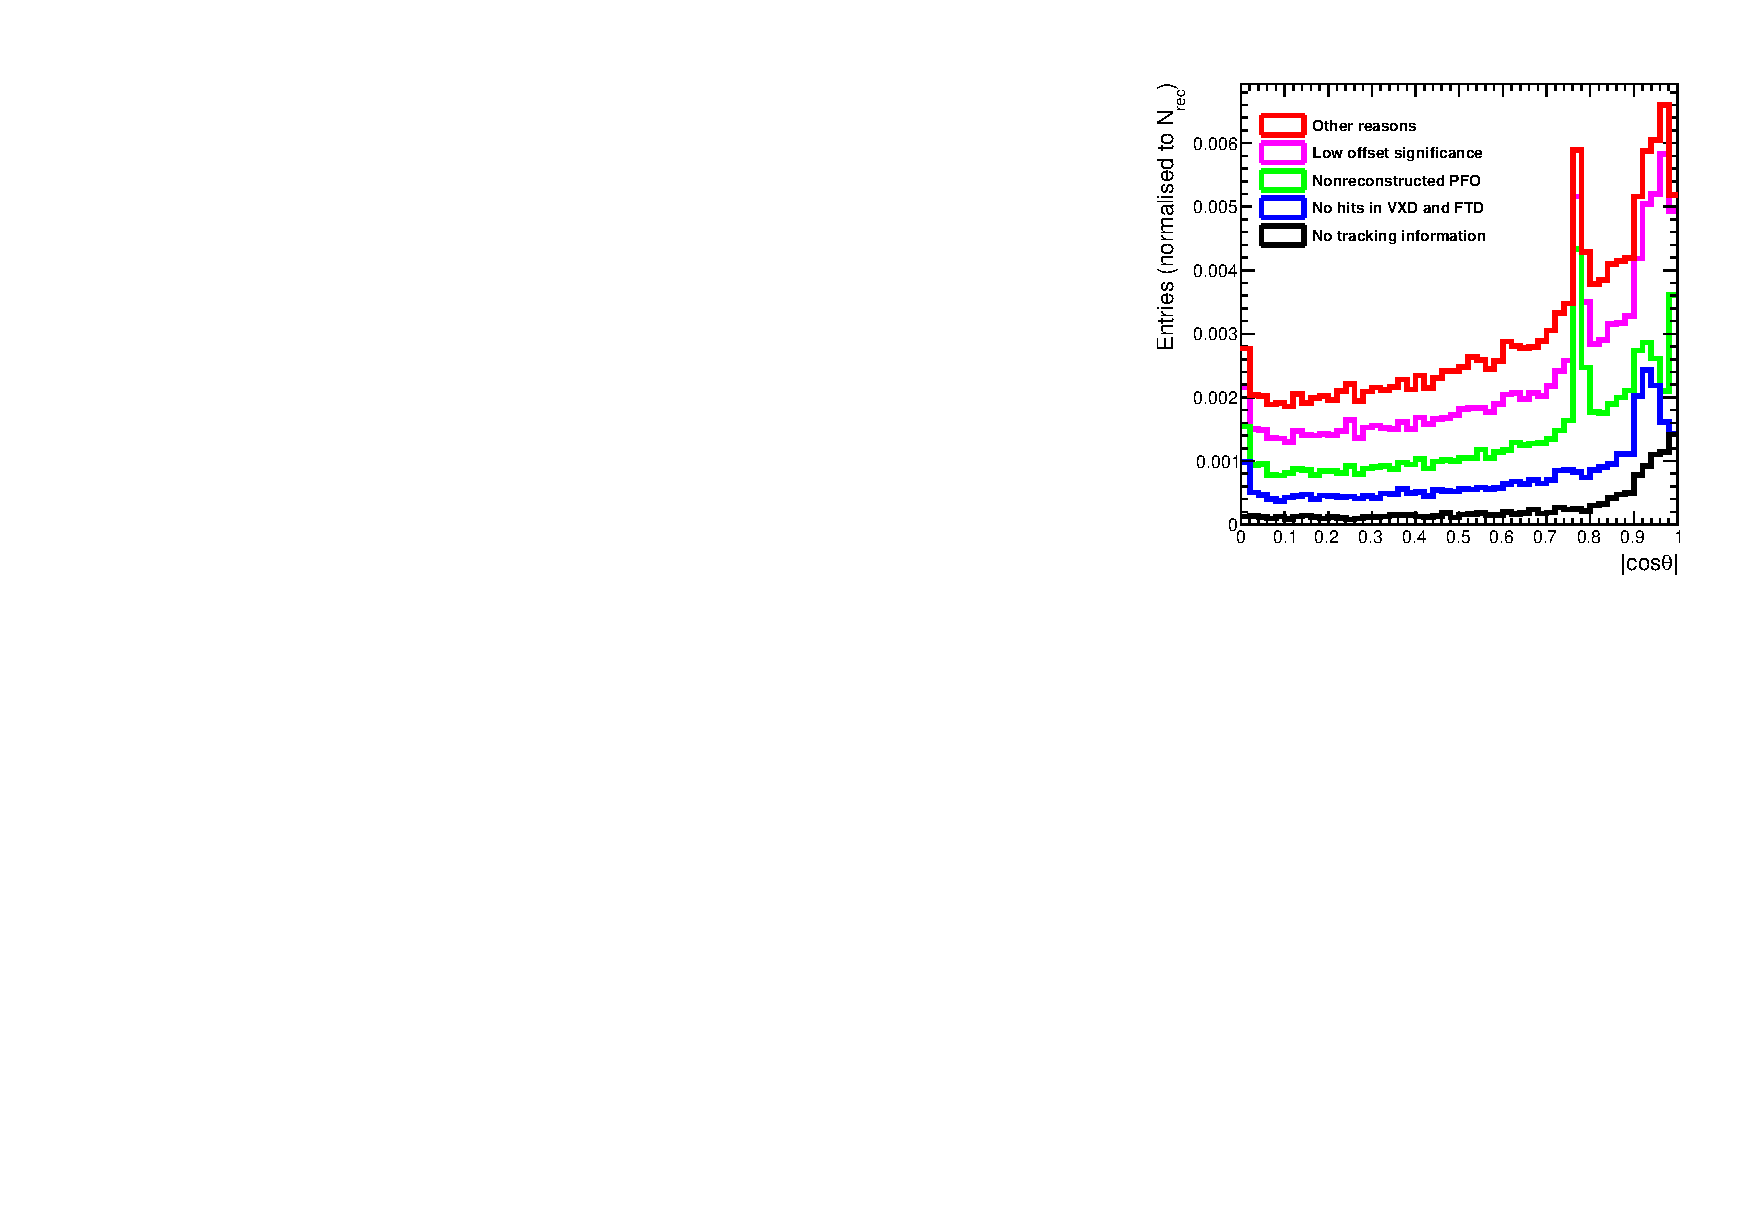
\includegraphics[width=0.95\textwidth]{ILD/plots/missed-tracks.pdf}
\caption{\label{fig:MissingTracks_cos_3} }
\end{subfigure}% 
  \begin{subfigure}{0.5\textwidth}
\centering
    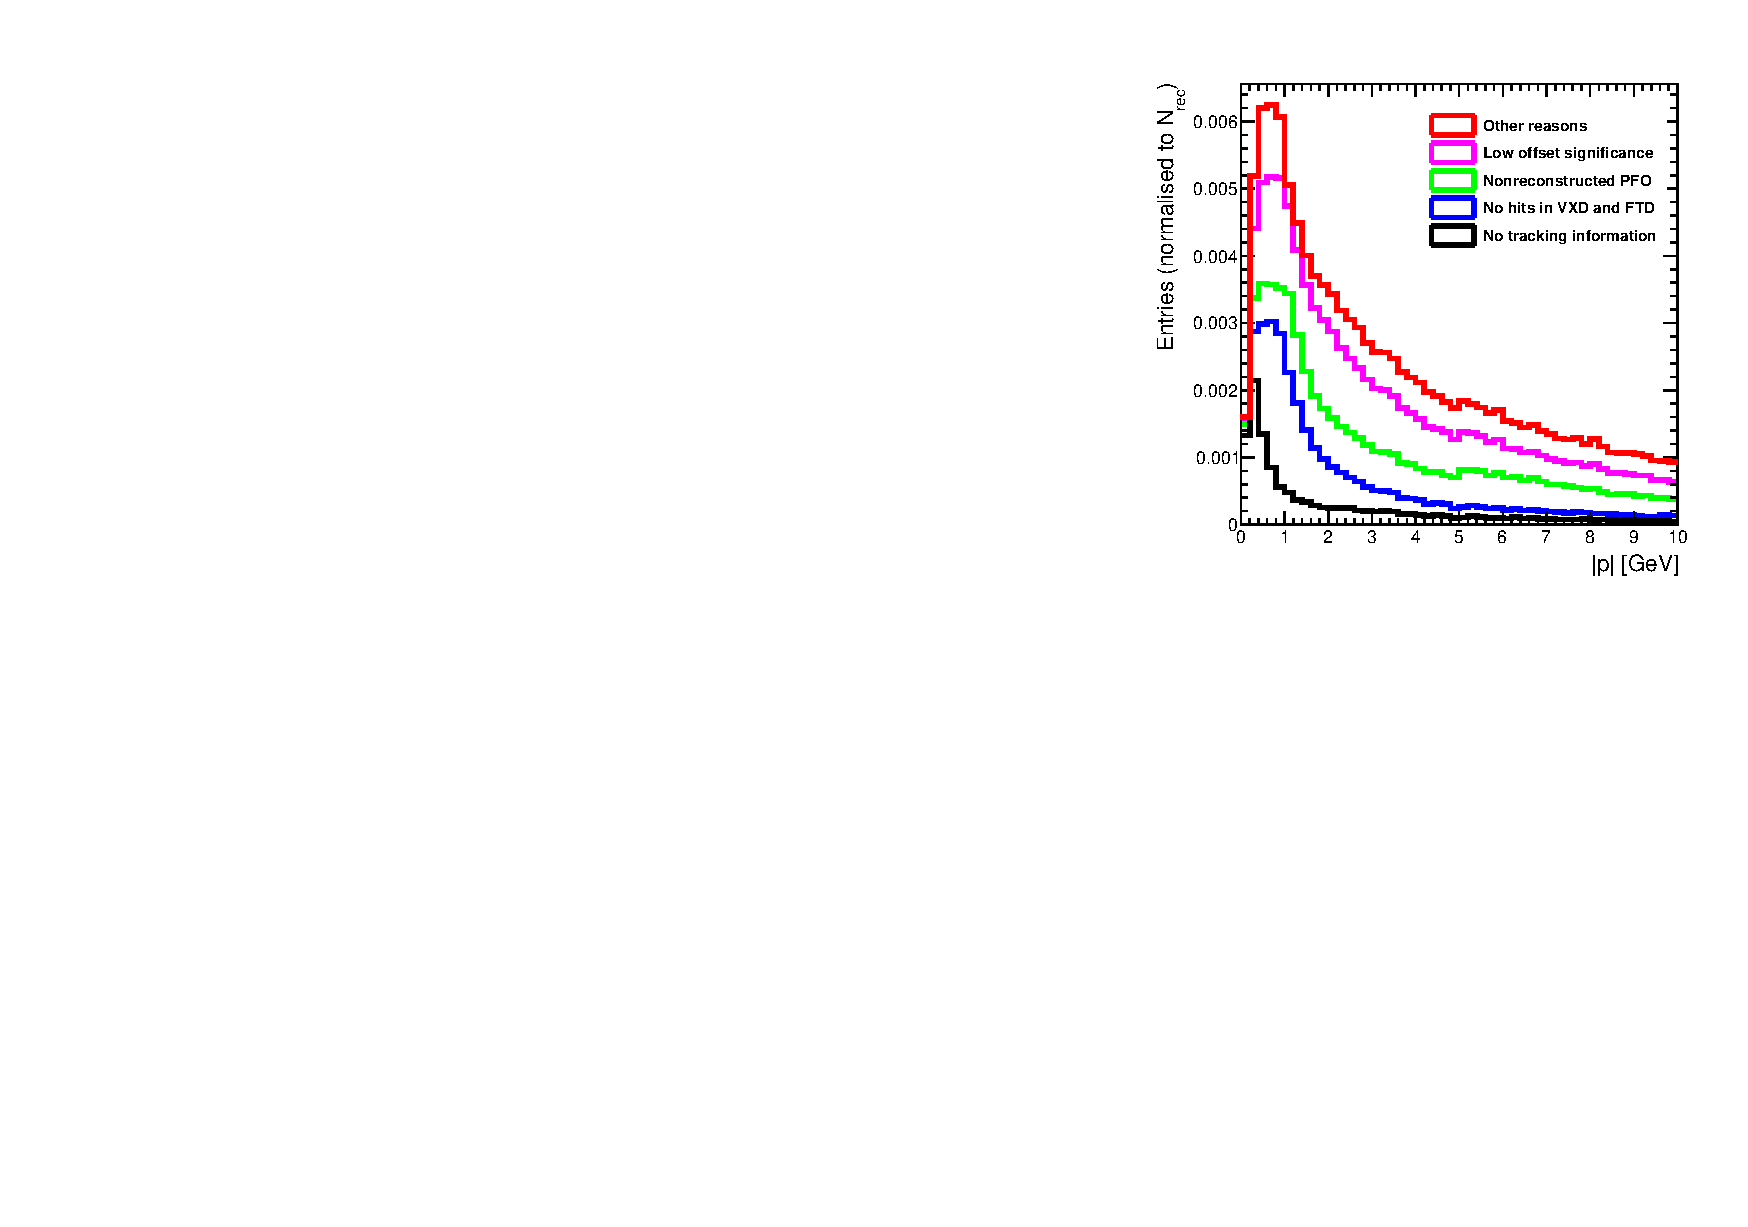
\includegraphics[width=0.95\textwidth]{ILD/plots/missed-momentum.pdf}
\caption{\label{fig:MissingTracks_p_3} }
\end{subfigure}
    \caption{\sl Polar angle~(a) and momentum~(b) distributions of the missing prongs subdivided into different categories. This is a stacked histogram. The peak at $|\cos\theta| = 0 $ is caused by the gap between TPC endplates, the peak at  $|\cos\theta| \approx 0.8$ is caused by barrel-endcap transition in the \ecal\ and the rapid increase at $|\cos\theta| \approx 0.9$ is caused by the barrel-endcap transition in the VXD and FTD system. }
    \label{fig:MissingTracks_3}
\end{figure}

\begin{figure}
	{\centering
		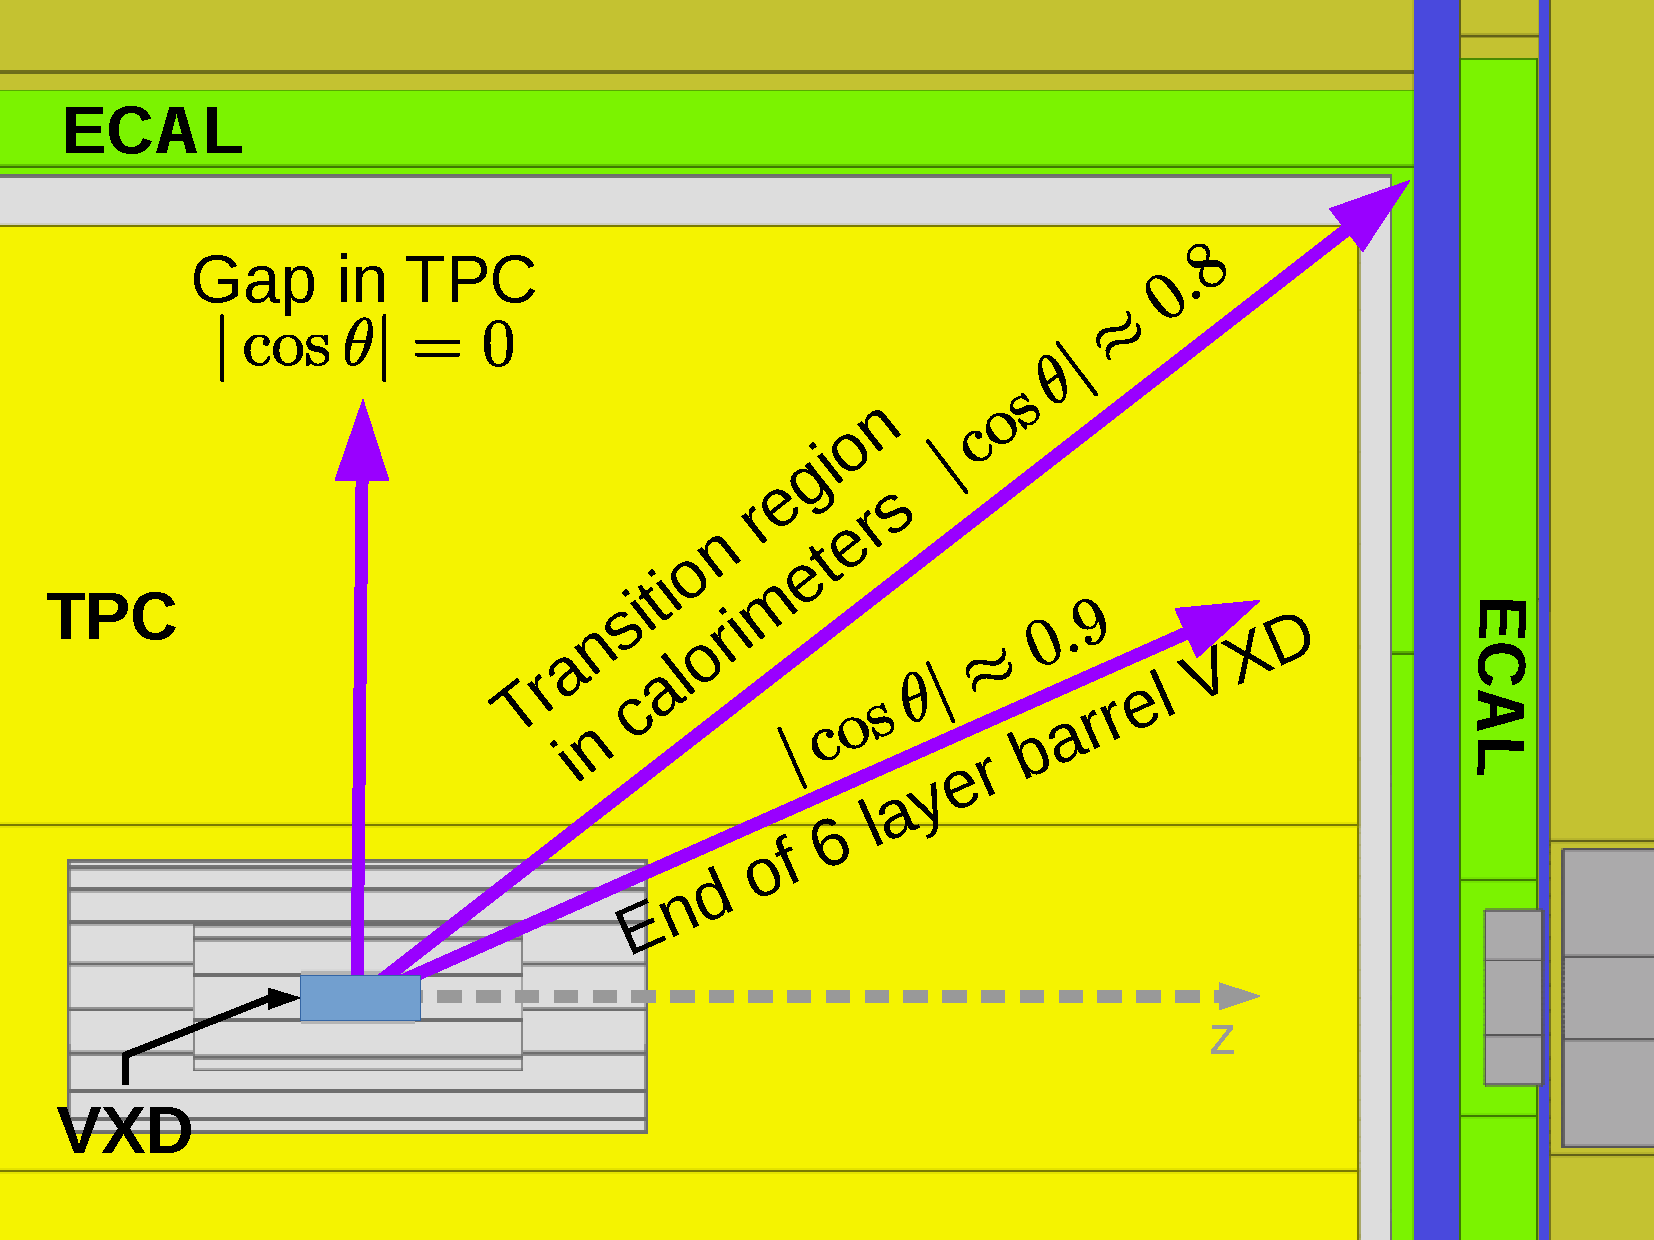
\includegraphics[width=0.55\textwidth]{ILD/graphics/directions.pdf}
		\caption{\sl Illustration of the polar angle directions in ILD layout, where one has peaks in the missing prongs distribution. 
		}
		\label{fig:ILDDirection_3}
	}
\end{figure}

These categories of the missing prongs can be illustrated by the polar angle histogram, shown in Fig.~\ref{fig:MissingTracks_cos_3}, which also reveals the following problems connected to the ILD geometry, see Fig.~\ref{fig:ILDDirection_3}:
\begin{itemize}
\item Small peak at $|\cos\theta| = 0$ is caused by the TPC cathode gap. 
\item Large peak at $|\cos\theta| \approx 0.8$ is caused by the PandoraPFO, which fails to connect a well reconstructed track with an offset to a segmented cluster located in the calorimeter barrel-endcap transition. This problem is specific to the b-hadron tracks;
\item Increase at $|\cos\theta| \approx 0.9$ correspond to the end of the full 3 double layer VXD acceptance, resulting in an increase in the impact parameter uncertainties of the reconstructed tracks. %caused by a connection problem between the VXD track segments, which are in the acceptance region of the two double-sided VXD layers, and the FTD track segments.
\end{itemize}

The recoverable prongs are those, which were lost because of the reconstruction problems, like the problems with the PFO creation, and not by the limited detector acceptance.  

%%%%%%%%%%%%%%%%%%%%%%%%%%%%%%%%%%%%%%%%%%%
%%%%%%%%%%%%%%%%%%%%%%%%%%%%%%%%%%%%%%%%%%%
%%%%%%%%%%%%%%%%%%%%%%%%%%%%%%%%%%%%%%%%%%%
\subsection{Vertex charge recovery}
\label{sec:VtxRecovery}
The objective of the vertex recovery algorithm is to add accurately the missing prongs to the reconstructed vertices, without contamination by the particles with non b-hadron origin or the background particles. 

%The most important observable for any vertexing algorithm is the particle offset $\epsilon$.
%The uncertainty on the offset $\sigma$ for a given reconstructed charged particle can be computed as 
%\begin{equation}
%	\sigma = \sqrt[]{\sigma_{d_{0}}^2 + \sigma_{z_0}^2},
%%\end{equation}
% 


In this study we use the following definition of the offset significance:

\begin{equation}
	\epsilon/\sigma = |\frac{d_0}{\sigma_{d_0}}| + |\frac{z_0 }{ \sigma_{z_0}}|,
\end{equation}
where $\sigma_{d_{0}}$ and $\sigma_{z_0}$ are the covariance matrix elements, provided by the track reconstruction algorithms.
The offset significance value depends strongly on the momentum of the particle, its polar angle and number of assigned VXD or FTD hits . 

Typically, the b-hadron prongs are generated with large offsets (Fig.~\ref{fig:GenHadronParams_b_3}), but the reconstruction can miss a reconstructed prong if it has a small offset significance. 
Hence, one needs another spatial separation variable, combined with the offset significance $\epsilon/\sigma$. 

%Another separation variable can make use of the reconstructed vertex position and the reconstructed track candidate parameters. 

The particle trajectory bending because of magnetic field is negligible at the small distance scales, like the b-hadron flight distance in Fig.~\ref{fig:GenHadronParams_b_3}. 
Therefore, in this studies, the reconstructed track helix is approximated by the reconstructed vector of particle momentum. 

Suppose, one has a reconstructed secondary vertex in a position $\vec{s}_{vtx}$ and a prong candidate with a momentum $\vec{p}$ and a track reference point $\vec{t}_0$, which is computed from track parameters $d_0$ and $z_0$.
This study uses an angle $\alpha$, as a second separation variable, defined as an angle between the particle momentum $\vec{p}$ and the vector of difference between the vertex position $\vec{s}_{vtx}$ and the track reference point $\vec{t}$. The angle $\alpha$ is illustrated in Fig.~\ref{fig:VtxRecovery_3}.

\begin{figure}
{\centering
    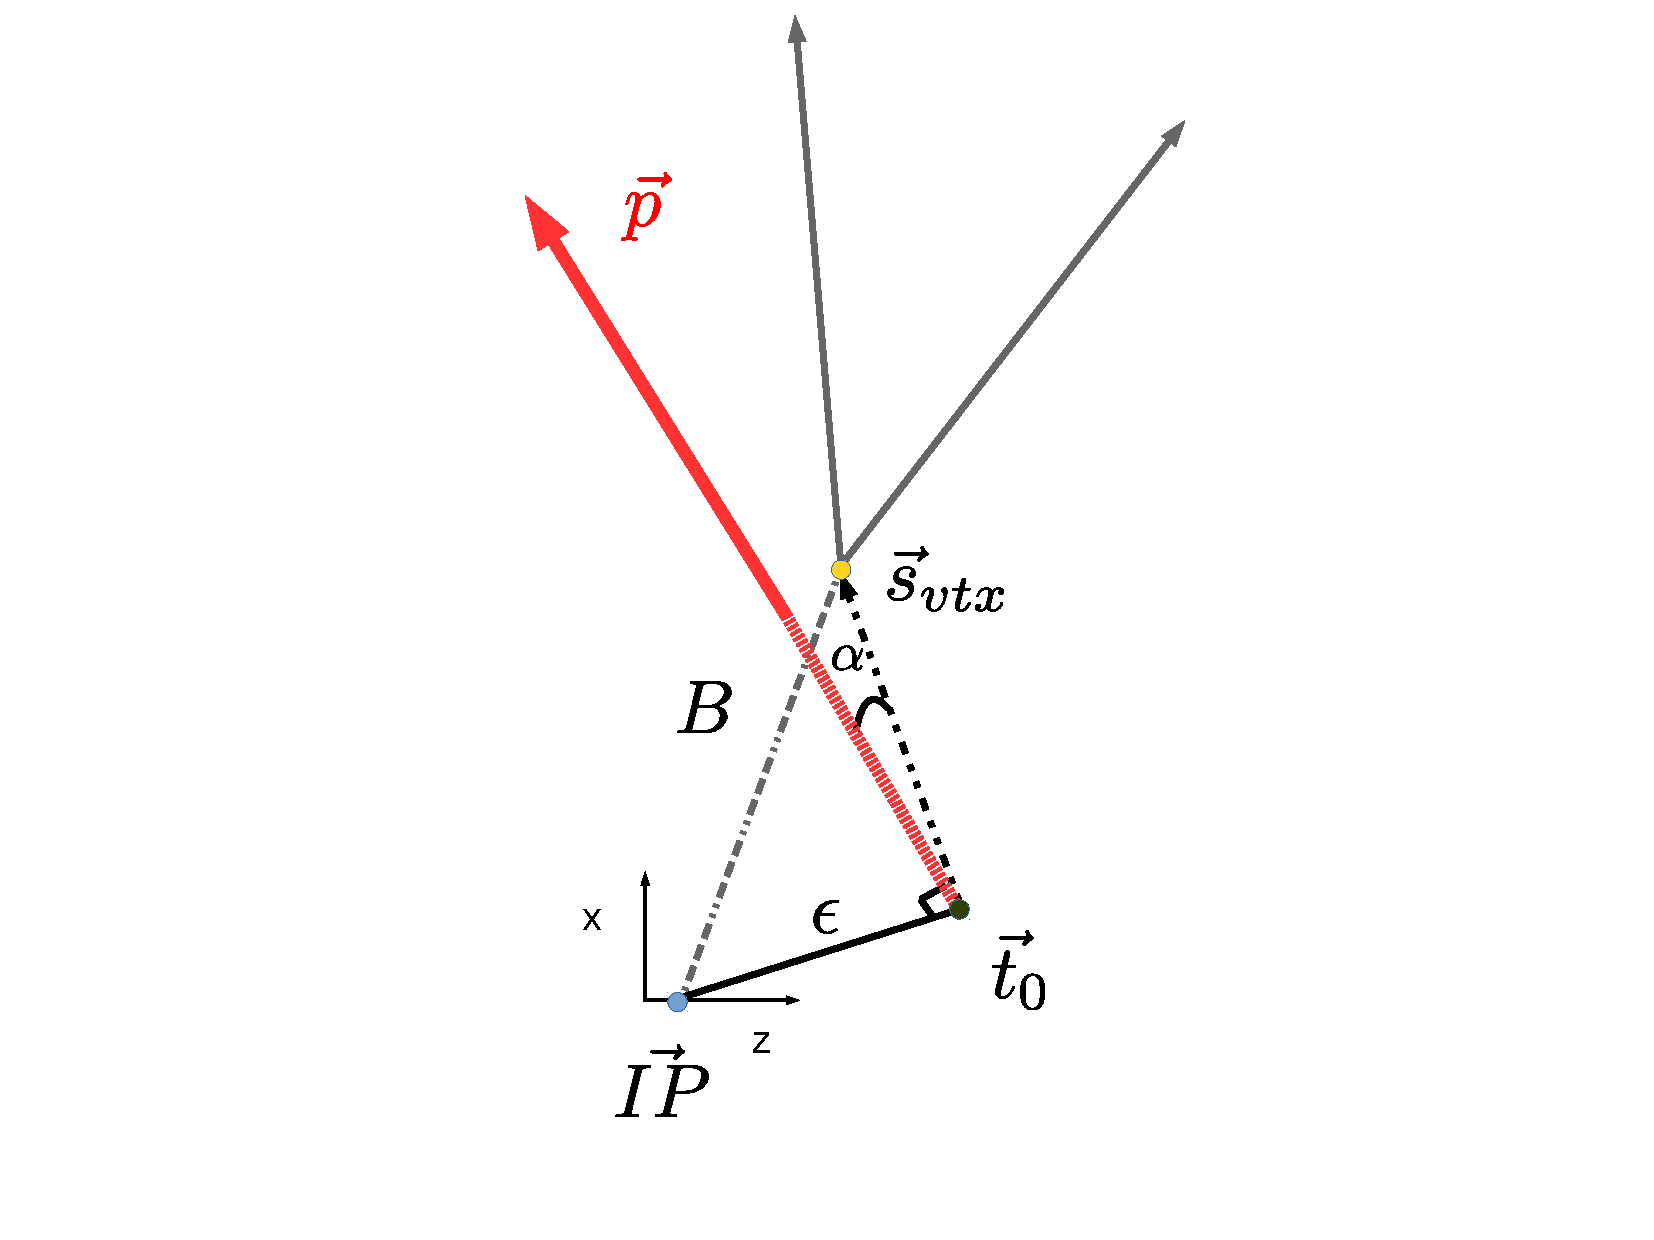
\includegraphics[width=0.75\textwidth]{ILD/plots/recovery-graph.pdf}
    \caption{\sl Illustration of the chosen separation variables of the vertex charge recovery algorithm, where $\vec{p}$ is a vector of a given particle momentum, $B$ is a flight distance of a b-hadron, $\vec{IP}$ is a primary vertex position, $\vec{t}$ is a reference point of a given particle, defined in \cite{bib:LCIOtrack}, $\alpha$ is the angle between $\vec{p}$ and $\vec{s}_{vtx}$ and $\epsilon$ is an offset distance of the particle. %Right: Same comparison, but after a cut on the b-tag$> 0.8$ and a cut on the b-hadron momentum more than 20\,GeV. The diagonal contains 55\% of the jets after the cuts.
    }
    \label{fig:VtxRecovery_3}
  }
\end{figure}

An algorithm, called VertexChargeRecovery, was developed to increase the b-quark charge purity by adding the missing prongs to the reconstructed vertices.  For a given jet, which has at least one associated reconstructed vertex, the VertexChargeRecovery has the following procedure:

\begin{itemize}
\item Preparation of the prong candidates - the algorithm uses all charged particles within a given jet as prong candidates. To recover the prongs, which has no reconstructed PFO, the program iterates throughout all reconstructed tracks and reconstructs them as charged PFOs without an associated calorimeter cluster. These new Particle Flow particles are used only if they have no duplicates in the previously selected jet particles;
\item All prong candidates are compared to the reconstructed prongs to avoid duplicates;
\item The separation variables $\alpha$ and $\epsilon$ are calculated for each prong candidate and a given reconstructed vertex;
\item The selection condition is defined using the $\alpha$ and $\epsilon$ distributions for true b-hadron prongs and background particles, which are displayed in Fig.~\ref{fig:RecoveryPurity_3}, suggest the following cuts:
\begin{equation}
\epsilon/\sigma > 2 + 25\cdot\alpha\text{ and } \alpha < 0.08.
\end{equation}
The recovery algorithm might have a different behavior in simulation, than in the real experiment, therefore, one should use a data-driven charge purity measurements, described in Sec.~\ref{sec:ChargePurity}, to test and tune the recovery parameters.
\item The algorithm creates new reconstructed vertices with old and recovered reconstructed prongs and links them to a given jet.
\end{itemize}

\begin{figure}
	\centering
	\begin{subfigure}{0.33\textwidth}
		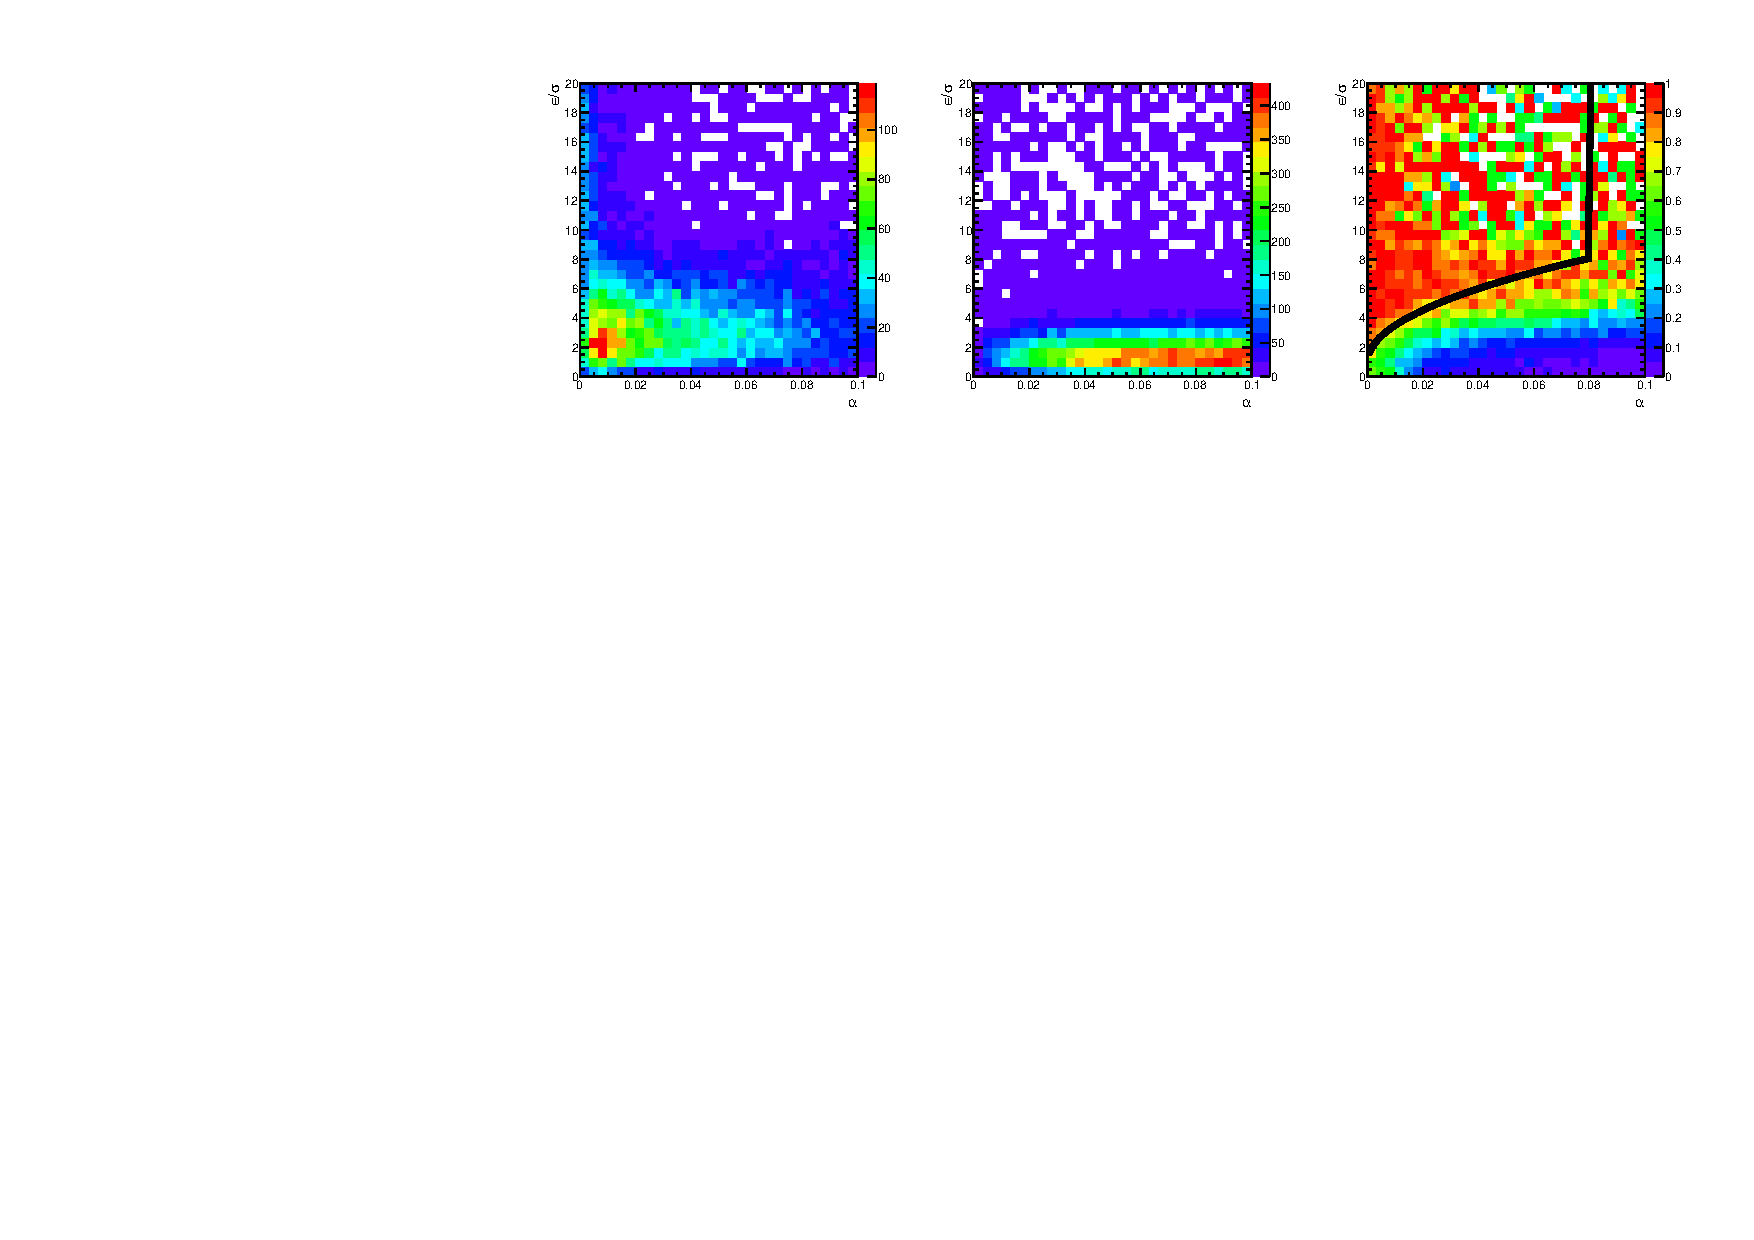
\includegraphics[clip, trim=0.1cm 0cm 13.8cm 0cm,width=0.99\textwidth]{ILD/plots/recovery-purity.pdf}
		\caption{\label{fig:RecoveryPurity_a_3} Missing particles}
	\end{subfigure}% 
	\begin{subfigure}{0.33\textwidth}
		\centering
		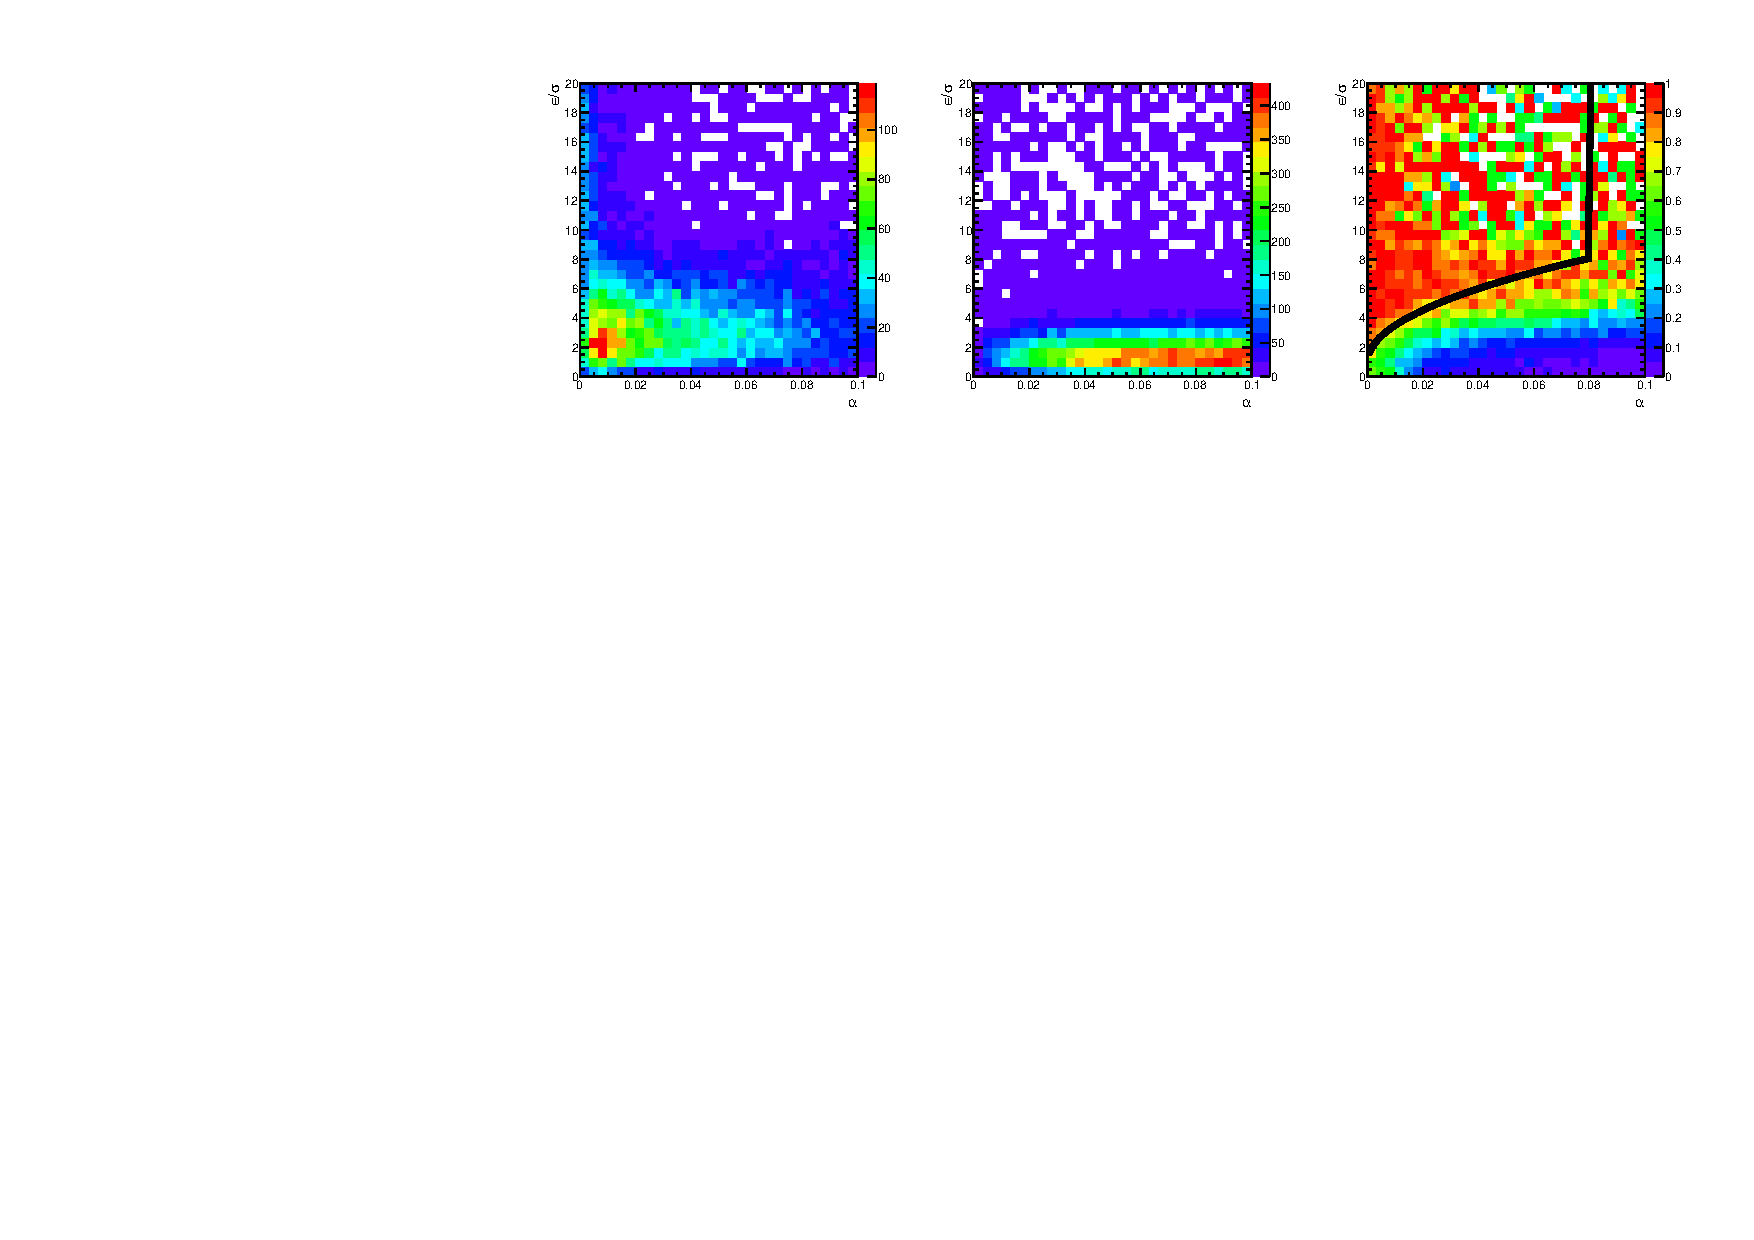
\includegraphics[clip, trim=6.78cm 0cm 7.1cm 0cm,width=0.99\textwidth]{ILD/plots/recovery-purity.pdf}
		\caption{\label{fig:RecoveryPurity_b_3} Background}
	\end{subfigure}
	\begin{subfigure}{0.33\textwidth}
		\centering
		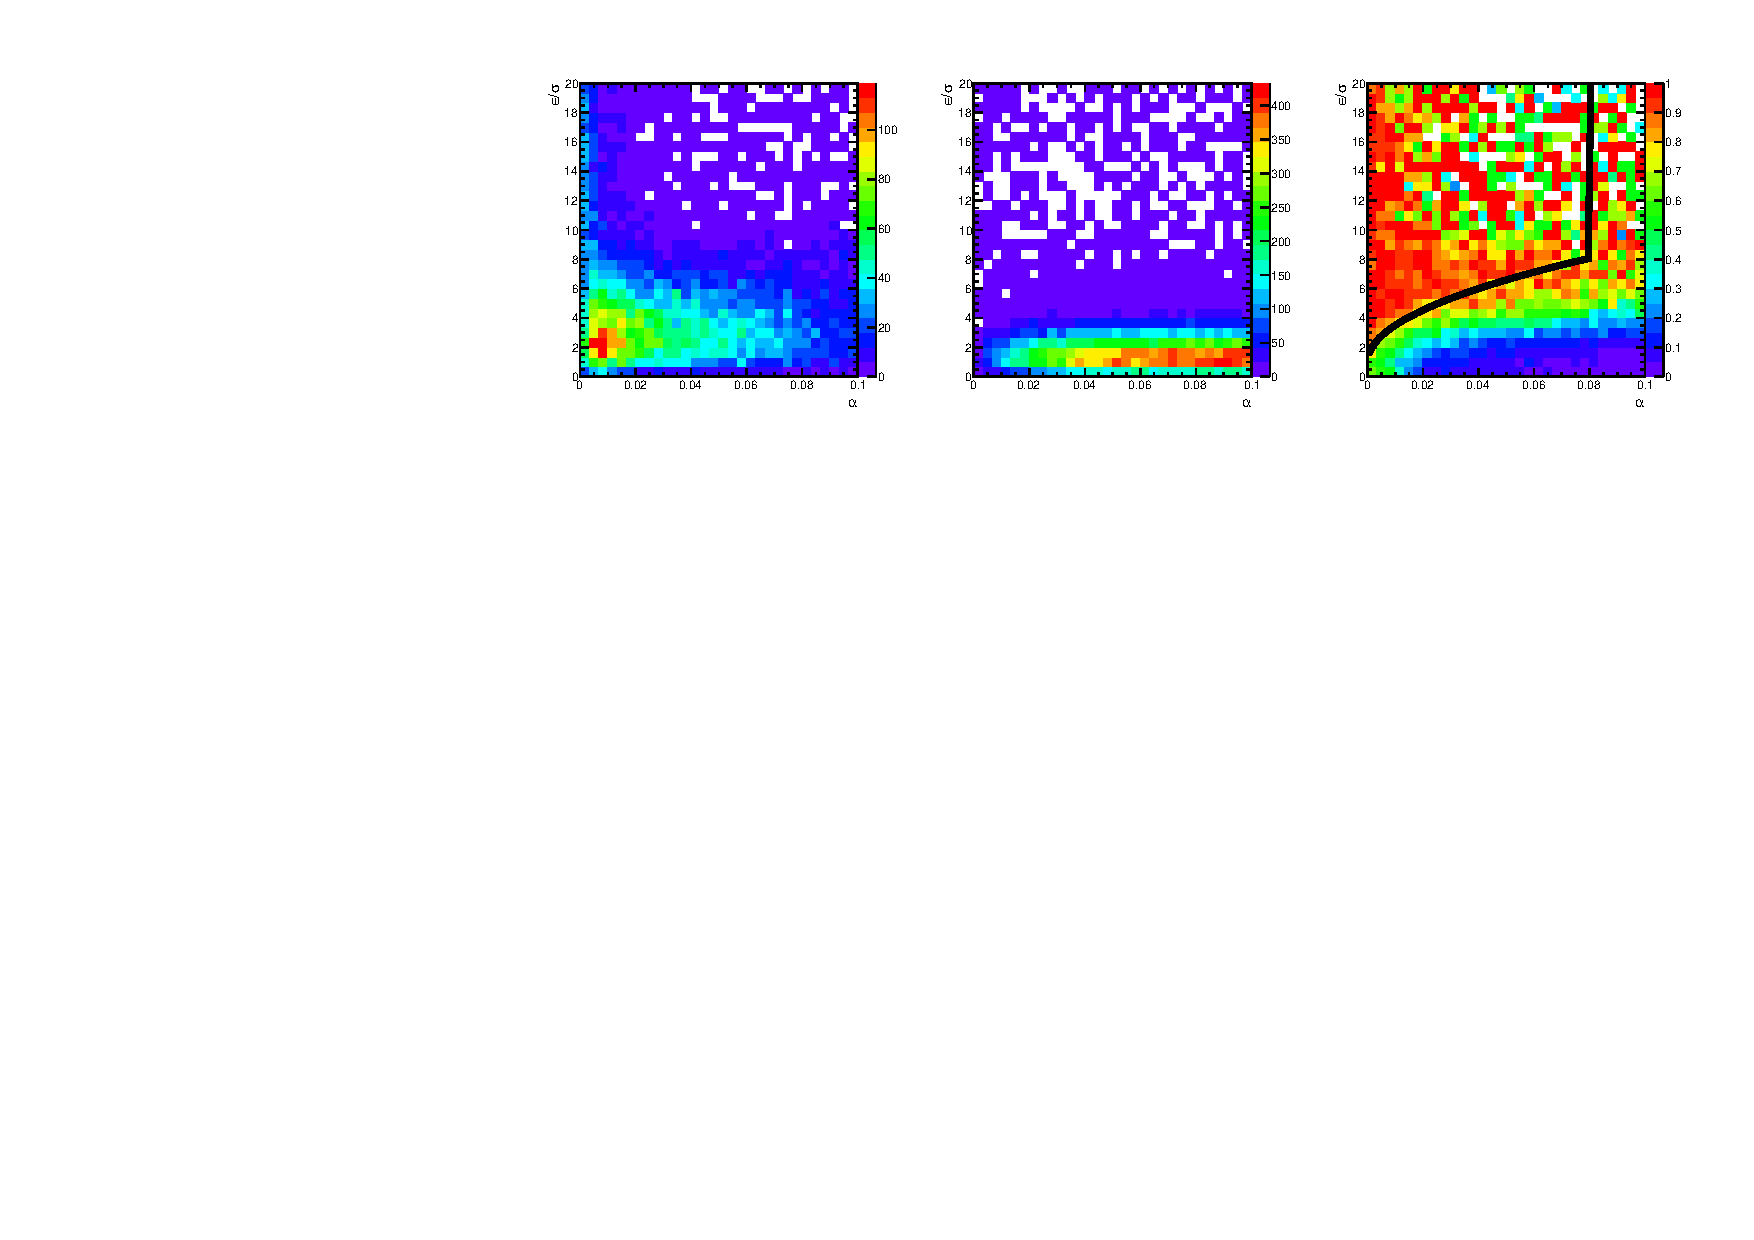
\includegraphics[clip, trim=13.5cm 0cm 0.4cm 0.cm,width=0.99\textwidth]{ILD/plots/recovery-purity.pdf}
		\caption{\label{fig:RecoveryPurity_c_3} Purity map}
	\end{subfigure}
	\caption{\sl Distribution of the separation variables, the angle $\alpha$ and the offset significance $\epsilon/\sigma$ for the missing generated prongs and the background charged particles. Purity map shows the highest concentration of the missing generated prongs as compare to all charged particles. The black line demonstrates the chosen cut function. }
	
	\label{fig:RecoveryPurity_3}
\end{figure}

The VertexChargeRecovery is made to have an output, identical to the output of the LCFI+ algorithms, which allows for a clear comparison of the b-quark charge reconstruction performance before and after vertex recovery usage.
%%%%%%%%%%%%%%%%%%%%%%%%%%%%%%%%%%%%%%%%%%%
%%%%%%%%%%%%%%%%%%%%%%%%%%%%%%%%%%%%%%%%%%%
%%%%%%%%%%%%%%%%%%%%%%%%%%%%%%%%%%%%%%%%%%%
\subsubsection{Results of the vertex recovery}

The simple algorithm of the vertex recovery is limited by the requirement of the presence of a reconstructed vertex and the reconstruction quality of a missing b-hadron prong. 
Nevertheless, this algorithm makes a significant improvement in the vertex reconstruction and the b-quark charge purity.

\begin{figure}
{\centering
    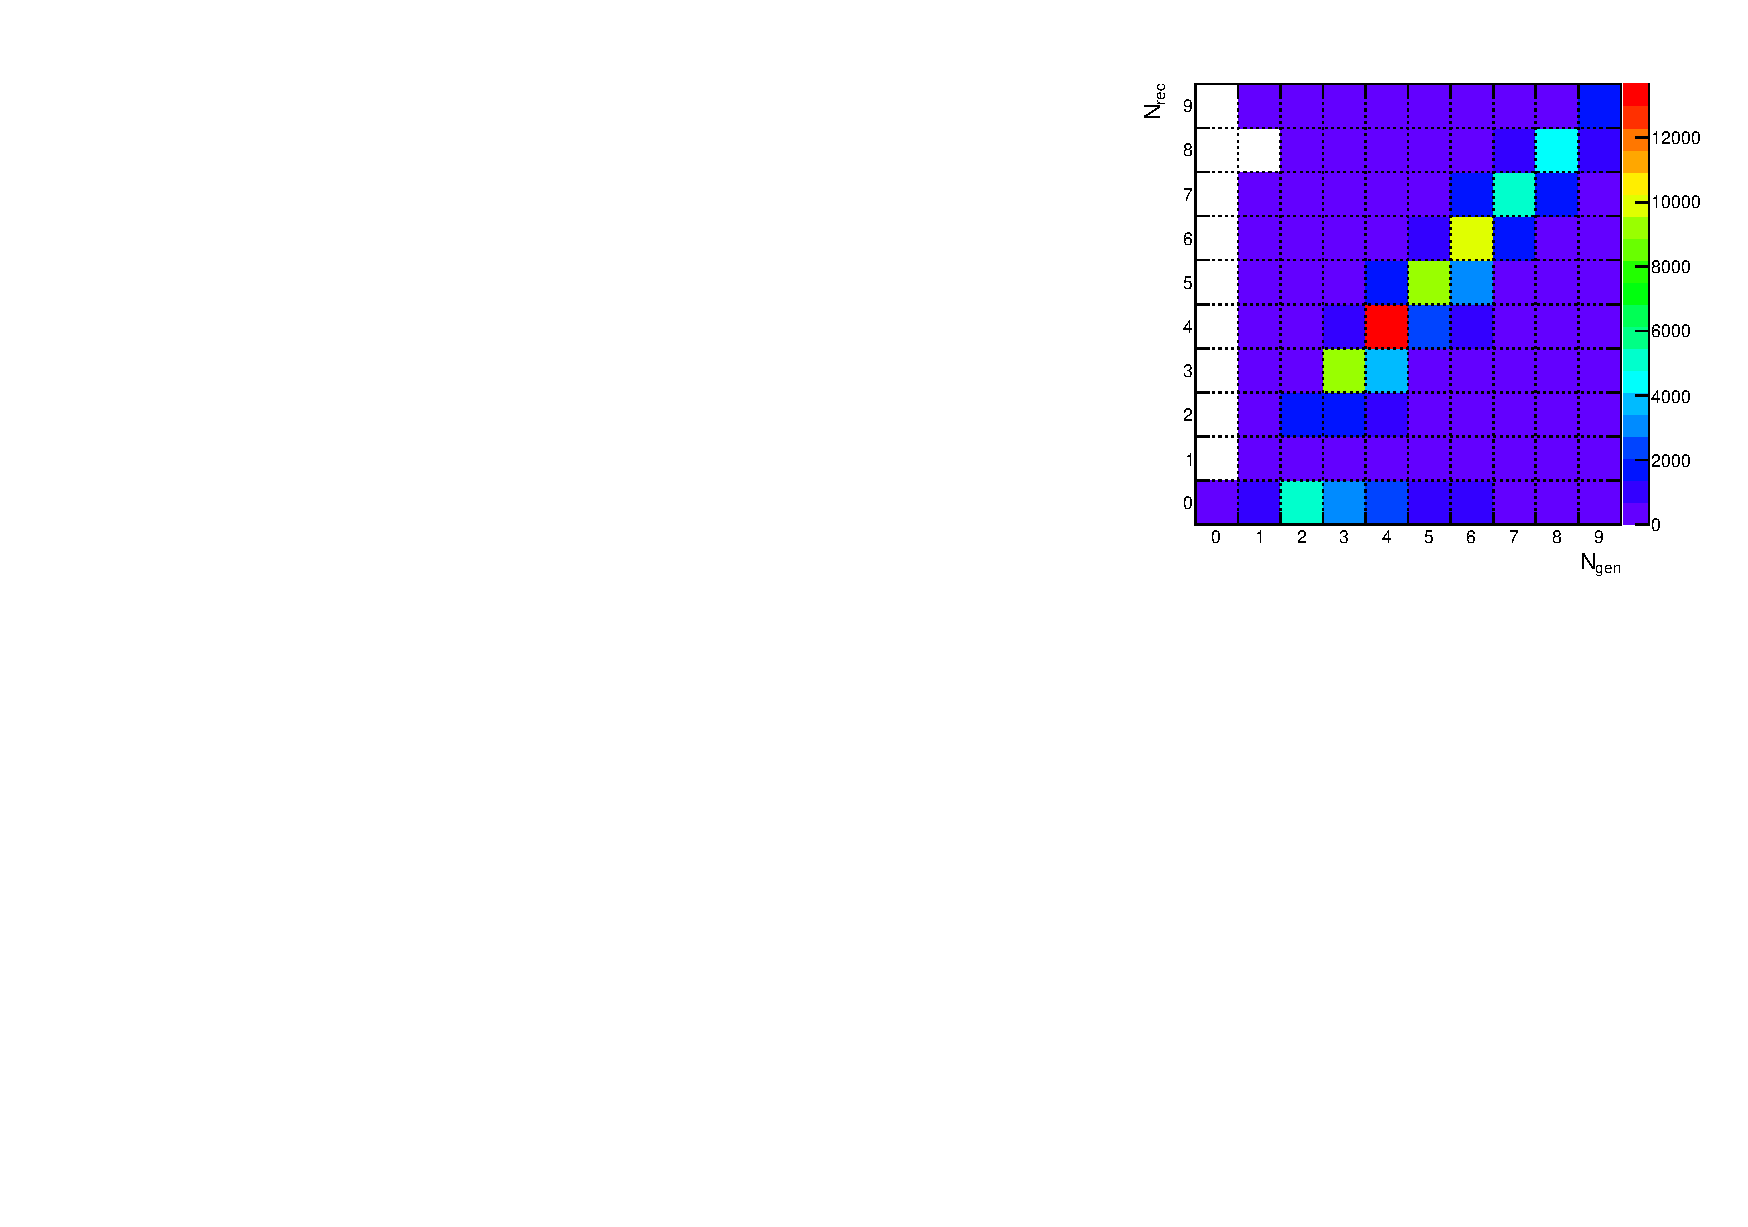
\includegraphics[width=0.55\textwidth]{ILD/plots/recovery-table.pdf}
    \caption{\sl Comparison of the number of reconstructed tracks $N_{gen}$ to the number of generated tracks $N_{rec}$ for a given b-jet after vertex charge recovery. The number of entries is color-coded for each cell. The fraction of the diagonal elements, which have the perfectly reconstructed vertices, is 62\% of all entries. The b-jets below diagonal have vertices with one or more particles missed by reconstruction. The row $N_{rec} = 0$ corresponds to the b-jets with no reconstructed vertices. %Right: Same comparison, but after a cut on the b-tag$> 0.8$ and a cut on the b-hadron momentum more than 20\,GeV. The diagonal contains 55\% of the jets after the cuts.
    }
    \label{fig:RecoveryTable_3}
  }
\end{figure}


The VertexChargeRecovery increases the fraction of correctly reconstructed jets from 49\% to 62\%, as it is illustrated in Fig.~\ref{fig:RecoveryTable_3}. 
This improvement is done by reducing the fraction of jets with $N_{rec} < N_{gen}$, below diagonal in Fig.~\ref{fig:RecoveryTable_3}. 
The slightly increased rate of jets with $N_{rec} > N_{gen}$ can be seen, which is an unavoidable shortcoming of the algorithm. 



\begin{figure}
\centering
\begin{subfigure}{0.5\textwidth}
    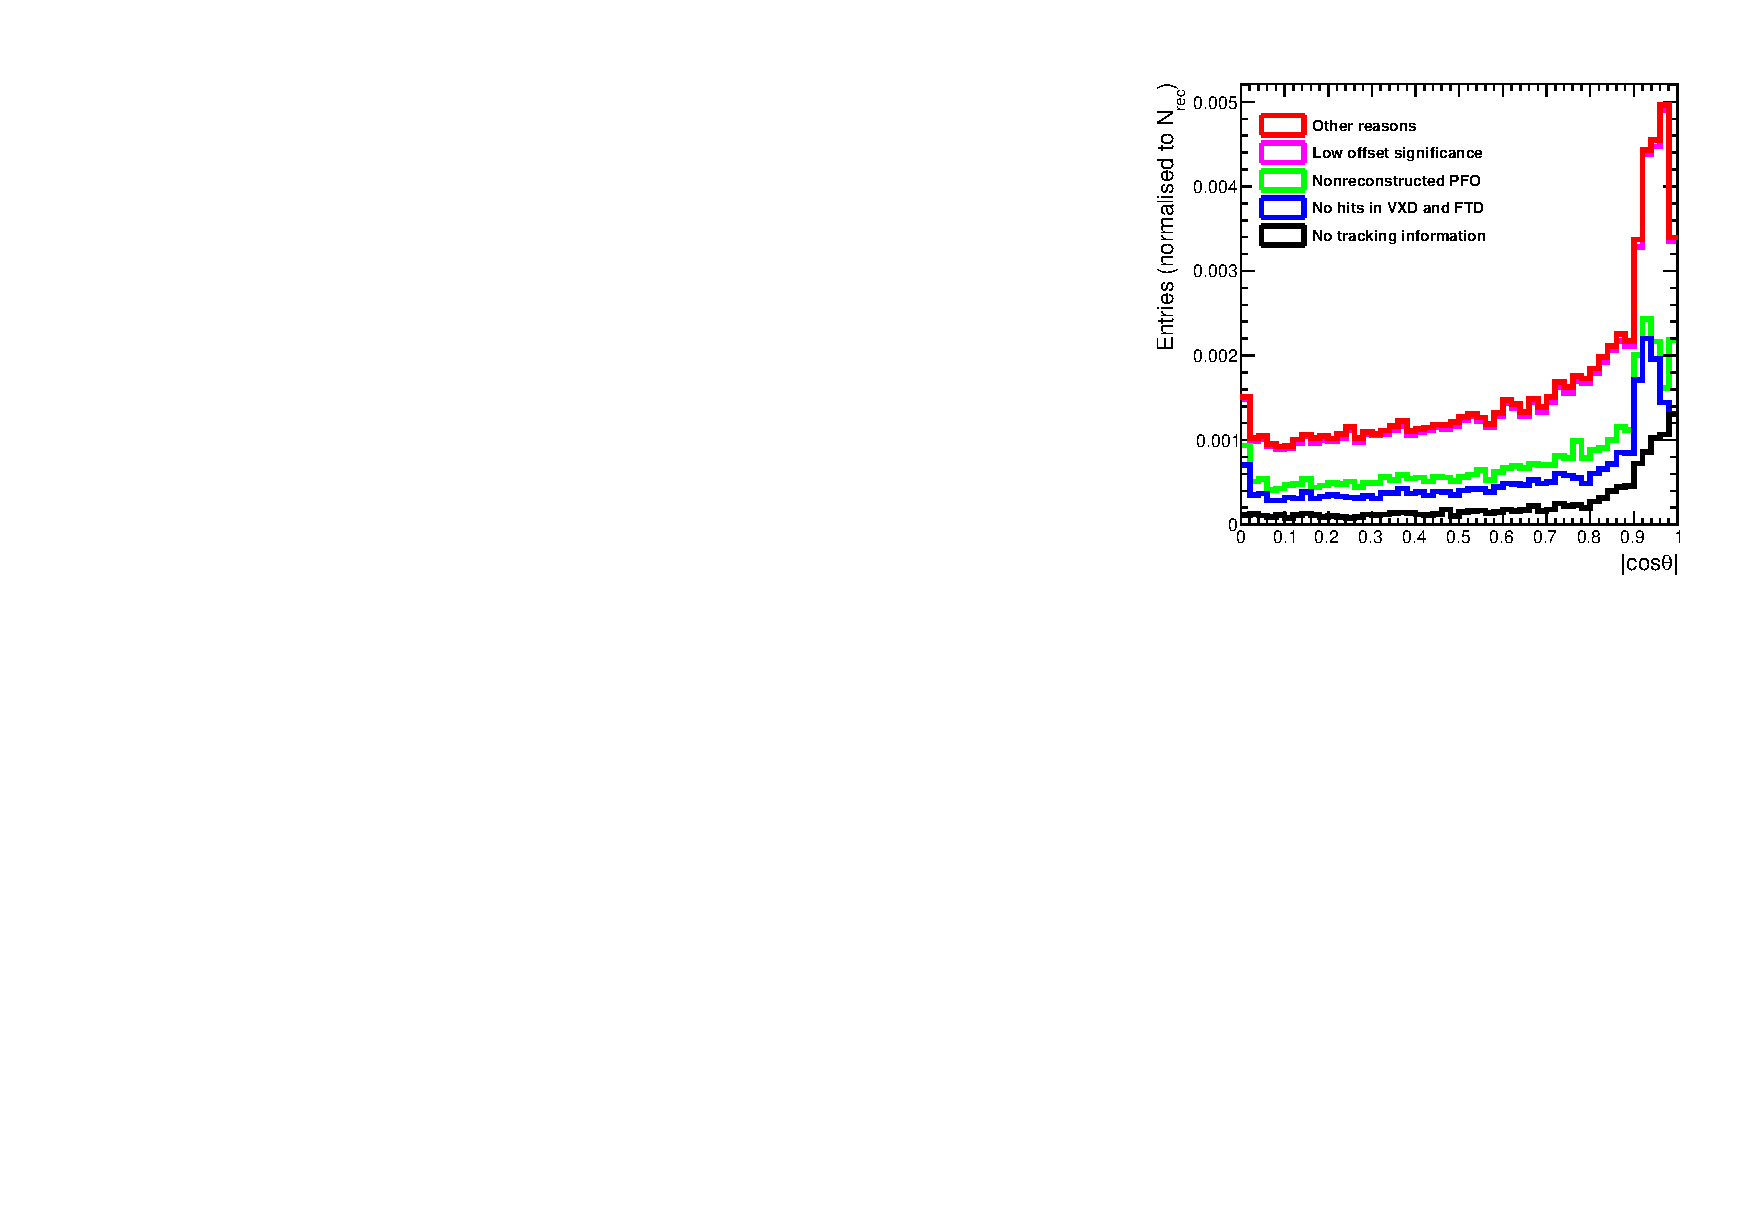
\includegraphics[width=0.95\textwidth]{ILD/plots/recovery-missed-cos.pdf}
\caption{\label{fig:RecoveryMissingTracks_cos_3} }
\end{subfigure}% 
  \begin{subfigure}{0.5\textwidth}
\centering
    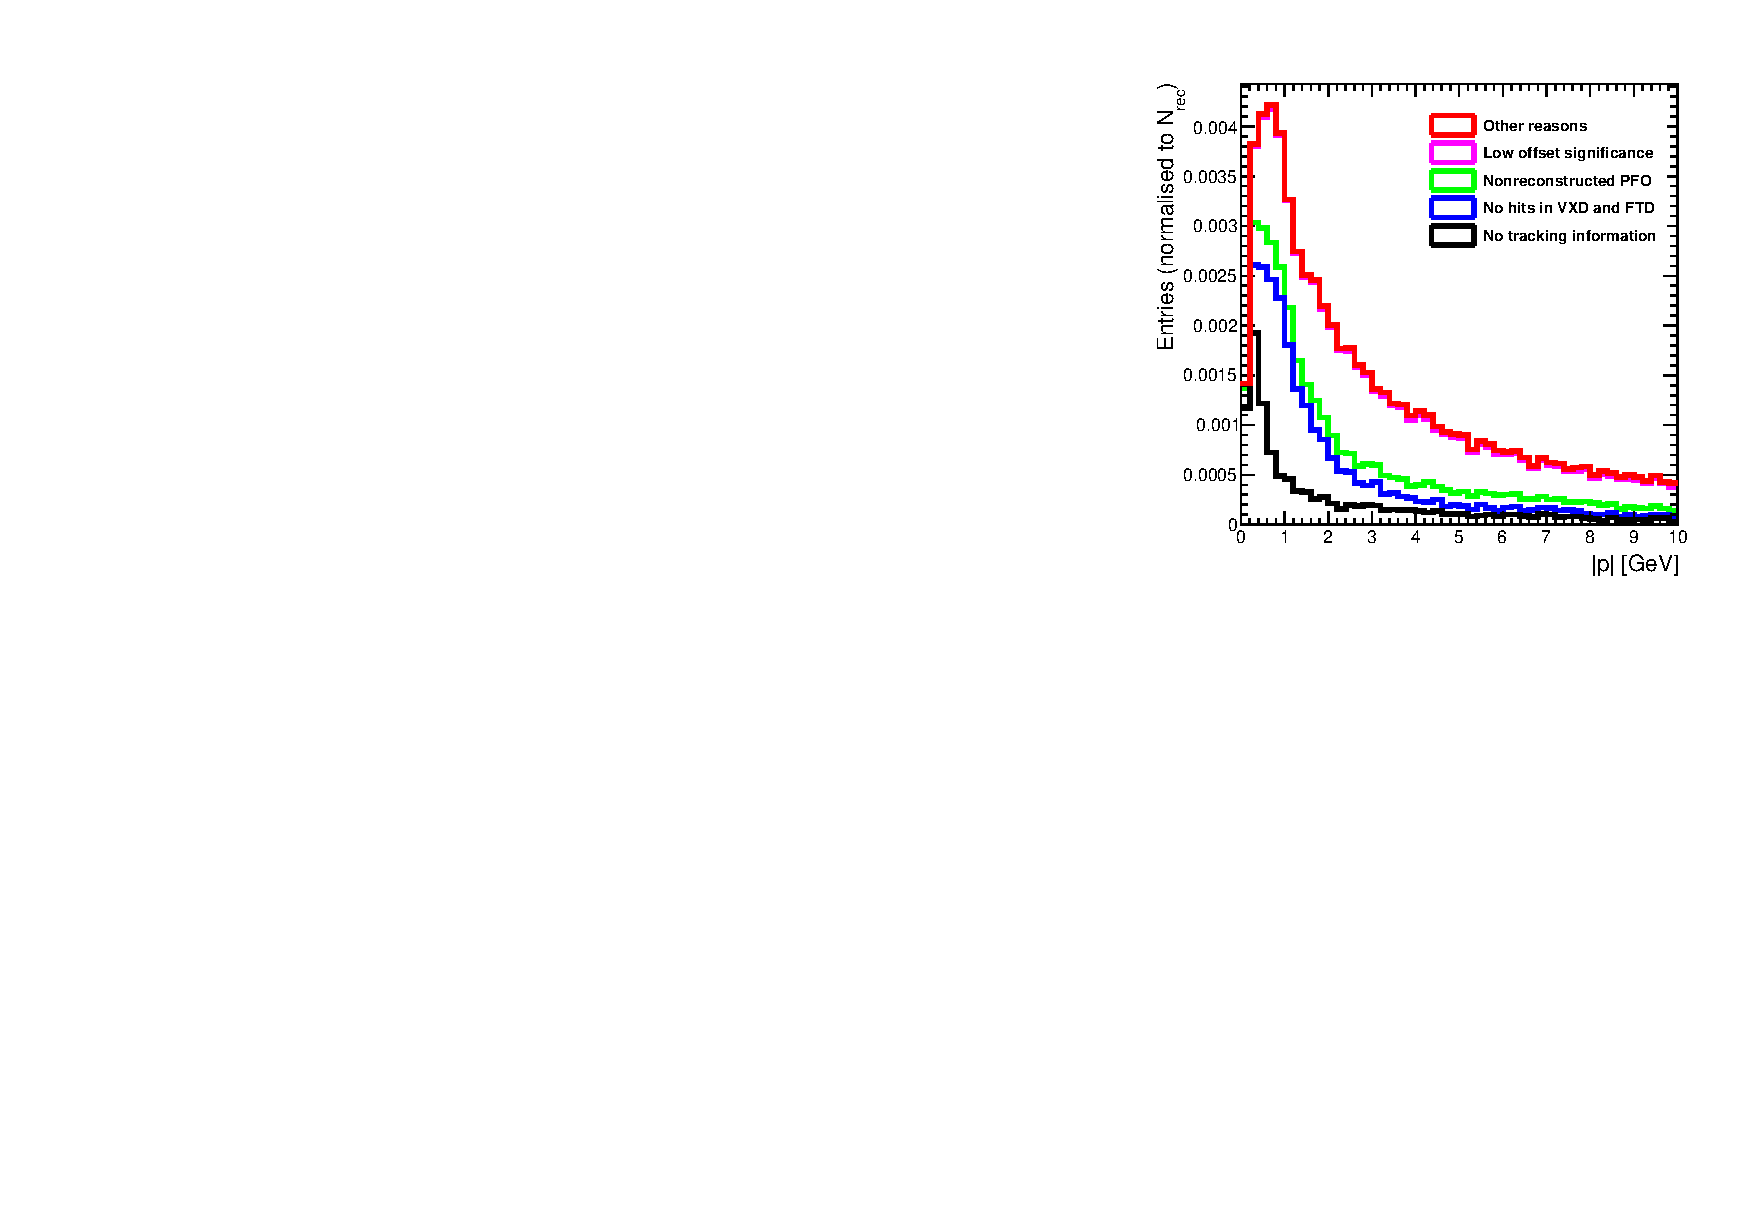
\includegraphics[width=0.95\textwidth]{ILD/plots/recovery-missed-p.pdf}
\caption{\label{fig:RecoveryMissingTracks_p_3} }
\end{subfigure}
    \caption{\sl Polar angle~(a) and momentum~(b) distributions of the missing prongs after vertex charge recovery subdivided into different categories. These are stacked histograms. }
    \label{fig:RecoveryMissingTracks_3}
\end{figure}

The vertex recovery decreases the fraction of missing prongs from 10.4\% to 6.2\%. The new polar angle and momentum distributions are shown in Fig.~\ref{fig:RecoveryMissingTracks_3}, from which one sees the following changes:
\begin{itemize}
\item The algorithm does not changes the categories of b-hadron prongs, which have no reconstructed tracks;
\item The reconstructed prongs with no assigned VXD or FTD hits are not recovered by the program;
\item The most of the missing prongs, which have no corresponding PFO are successfully associated to the correct reconstructed vertices;
\item The large peak of the missing prongs at $|\cos\theta| \approx 0.8$ is successfully eliminated;
\item The prongs in the region of the strong background, as can be seen in Fig.~\ref{fig:RecoveryPurity_3}, are not used by the program;
\item The missing prongs, which where lost by other means, are successfully recovered by the algorithm.
\item The vertex recovery can use all particles, even the ones with a small momentum, below 1\,GeV or outside the barrel VXD acceptance. 
\end{itemize}

%To resolve the inefficiencies, caused by the tracking, one can apply different VXD tracking algorithms, like minivector tracking. 

The central result of the algorithm is that it enhances the b-quark charge purity from 66\% to 73\%, despite increase of the contamination by the  background particles from 3\% to 4\%.
Figure~\ref{fig:RecoveryPurityComparison_3} demonstrates the improvement of the b-quark charge purity as function of the jet b-tag, reconstructed b-hadron momentum, $N_{rec}$ and the polar angle of the b-hadron  $|\cos\theta_{vtx}|$.
\begin{figure}
{\centering
    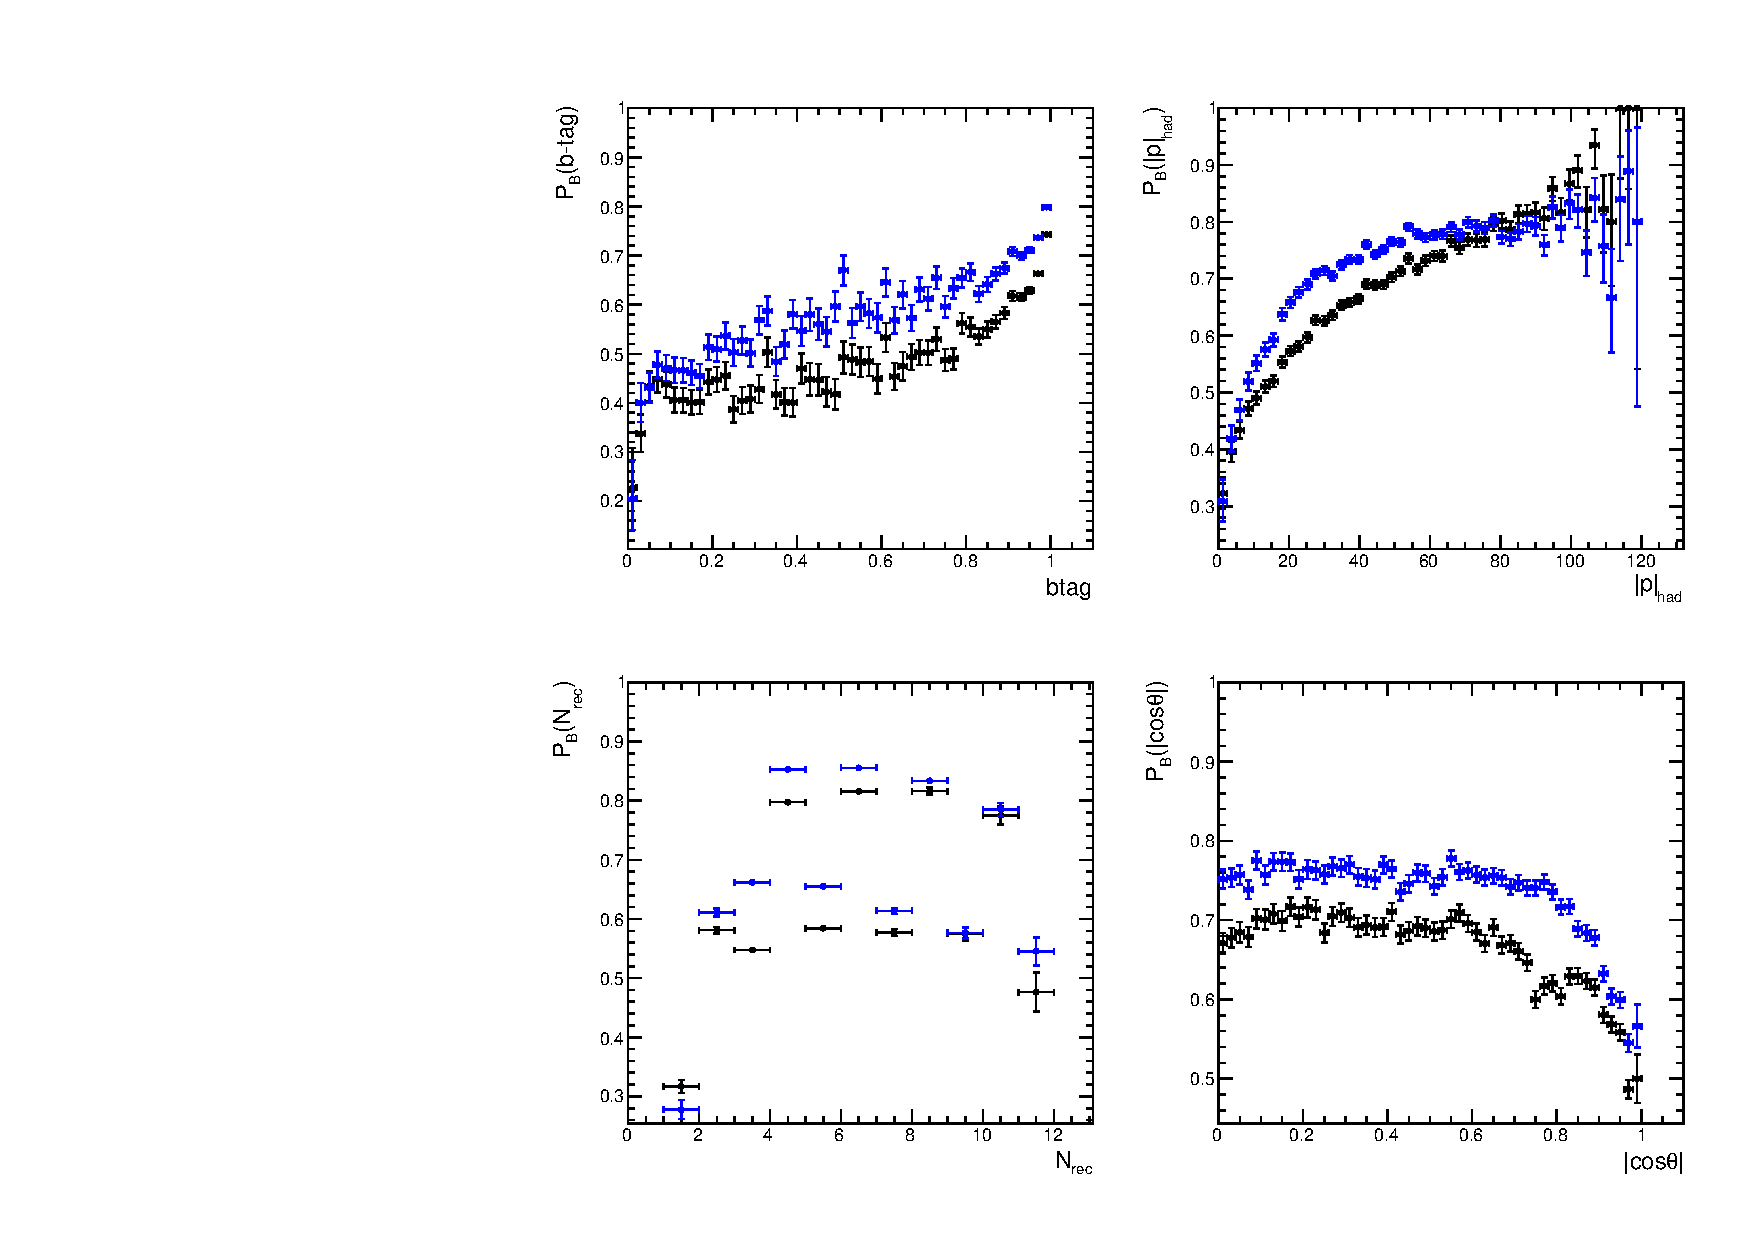
\includegraphics[width=0.95\textwidth]{ILD/plots/recovery-purity-comparison.pdf}
    \caption{\sl Comparison of the purity as function of the jet b-tag, reconstructed b-hadron momentum, $N_{rec}$ and the polar angle $|\cos\theta|$ before and after the vertex recovery algorithm.  
    }
    \label{fig:RecoveryPurityComparison_3}
  }
\end{figure}
One can see the following changes induced by the recovery algorithm:
\begin{itemize}
\item Jets with a high b-tag have higher chances to be recovered. The b-tag value strongly depends on the offsets of the reconstructed prongs, the low b-tag jets have less significant offsets of particles, which makes them  harder to recover. 
\item The algorithm improves the jets with a moderate reconstructed b-hadron momentum. %The algorithm should be tuned to work with highly collimated vertices produced by high momentum b-hadrons.
\item The large improvement can be seen for the jets or reconstructed b-hadrons with low number of reconstructed prongs, especially for $N_{rec}=3$.% For higher multiplicity, the algorithm should recover all tracks correctly, which is not trivial. Hence, almost no improvement is seen for the reconstructed b-hadrons with large $N_{rec}$.
\item The algorithm is capable to increase the purity in the barrel VXD acceptance and recover the non-reconstructed PFO particles at $|\cos\theta_{vtx}| \approx 0.8$. 
\end{itemize}
%The b-quark charge purity can be also increased by applying cuts on the reconstructed observables up to 80\% purity with 60\% efficiency or by application of MVA algorithm.

To summarize, the VertexChargeRecovery is able to significantly improve the b-quark charge purity and equalize it in the polar angle spectrum, which is crucial for the quark polar angle reconstruction. 
%%%%%%%%%%%%%%%%%%%%%%%%%%%%%%%%%%%%%%%%%%%
%%%%%%%%%%%%%%%%%%%%%%%%%%%%%%%%%%%%%%%%%%%
%%%%%%%%%%%%%%%%%%%%%%%%%%%%%%%%%%%%%%%%%%%
\subsection{Using the $dE/dx$ information}
\label{sec:Kaons}
A complementary method to measure the b-quark charge is to identify among the reconstructed b-hadron prongs the charged kaon $K^\pm$, which carry the information about the initial b-quark charge. 

The charged kaons have much higher mass than the charged pions and lower mass than protons, which makes possible to identify charged kaons by the energy deposition of the hits in the subdetectors. 

The most suitable device to calculate the energy deposition per distance passed, the $dE/dx$ value, is the ILD TPC due to its bulk gaseous environment. 


The $dE/dx$ as a function of the particle momentum and $|\cos\theta|$ for different hadrons is shown in Fig.~\ref{fig:dEdxBefore_3}. One can immediately spot the dependence of the $dE/dx$ value on the polar angle of the particles. This happens because of the knocked-out electron emittance or $\delta$-ray probability is increased with increasing length of the TPC track. Therefore, one needs to apply an angular correction to remove the angular dependence of the $dE/dx$ value, which is 
\begin{equation}
	\frac{dE}{dx}\to\frac{dE}{dx}\theta^{0.15},
    \label{formula:dEdxCorrection}
\end{equation}
where $\theta$ is the polar angle of the particle. 
This angular is known to be applied at other experiments, which have the TPC devices~\cite{bib:HARP}~\cite{buskulic:in2p3-00002096}.

The distributions of the $dE/dx$ as a function of particle momentum and $|\cos\theta|$ after the angular correction (\ref{formula:dEdxCorrection}) are displayed in Fig.~\ref{fig:dEdxAfter_3}.
%116.90%
\begin{figure}
{\centering
    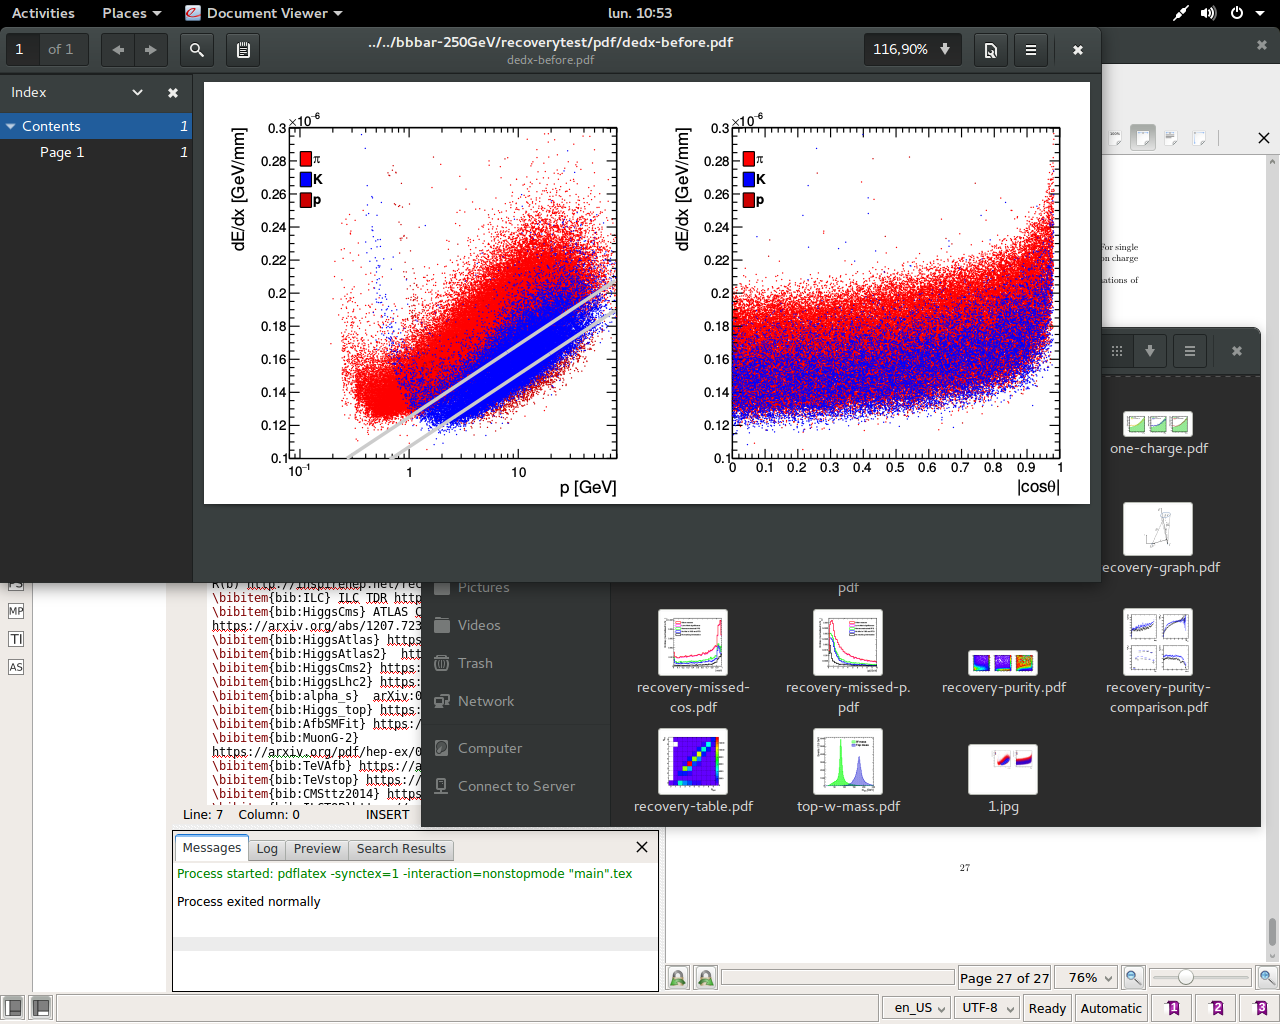
\includegraphics[clip, trim=8cm 18.5cm 7cm 4cm,width=0.95\textwidth]{ILD/plots/dedx-before.png}
    \caption{\sl The energy deposition per track length $dE/dx$ as function of the particle momentum, the particle polar angle $|\cos\theta|$ for different particles. Two gray lines separate out the region with a maximal kaon concentration. 
    }
    \label{fig:dEdxBefore_3}
  }
\end{figure}

\begin{figure}
{\centering
    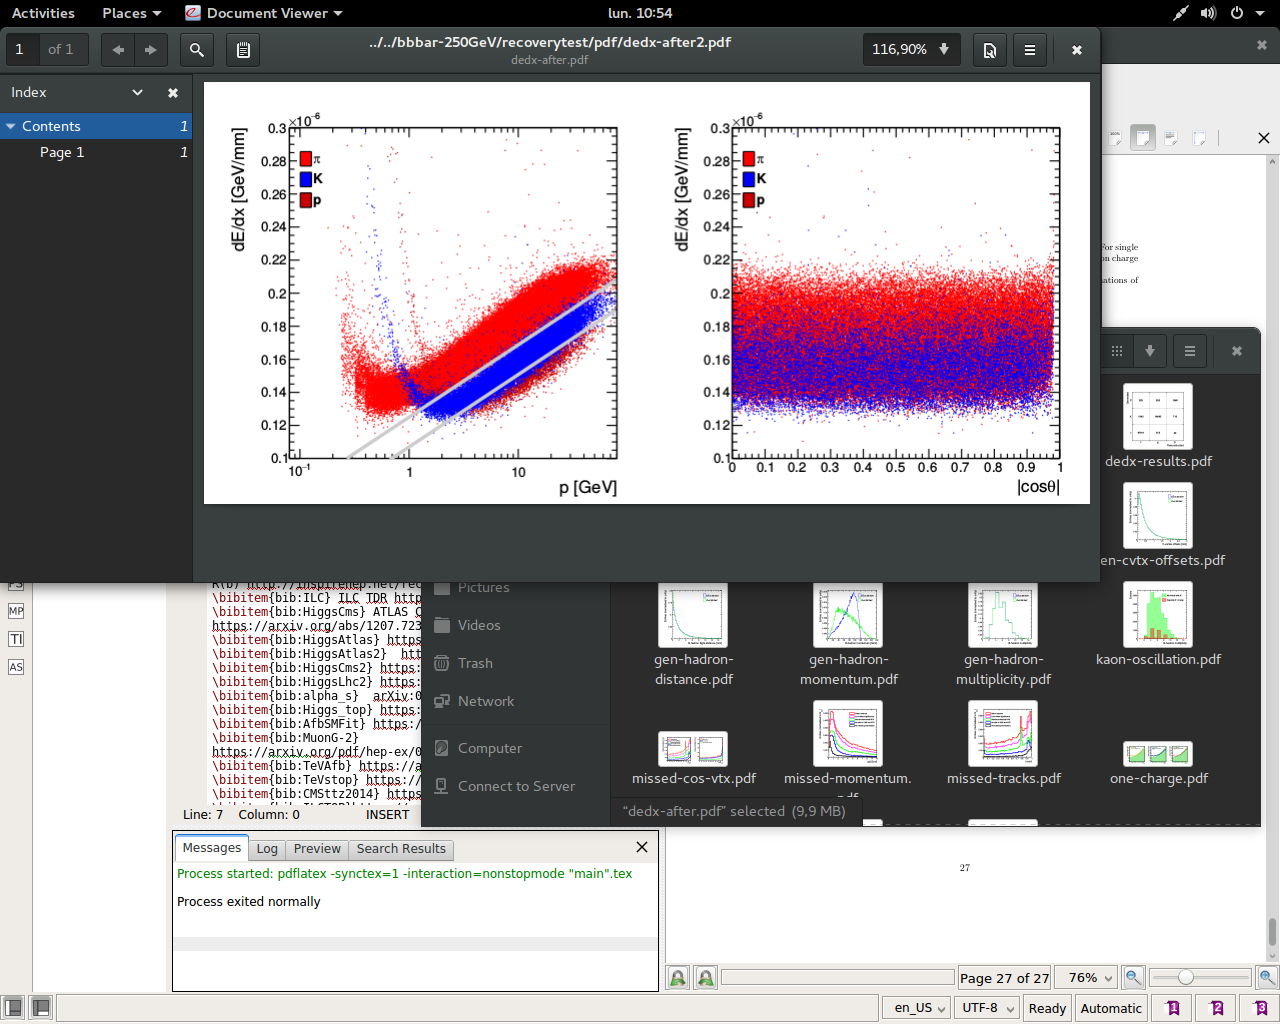
\includegraphics[clip, trim=8cm 18.5cm 7cm 4cm, width=0.95\textwidth]{ILD/plots/dedx-after.png}
    \caption{\sl The energy deposition per track length $dE/dx$ as function of the particle momentum, the particle polar angle $|\cos\theta|$ for different particles after application of the angular correction, described in text. Two gray lines separate out the region with a maximal kaon concentration. 
    }
    \label{fig:dEdxAfter_3}
  }
\end{figure}

A simple cut-based algorithm was developed to identify the particle type (PID) using $dE/dx$ information after angular correction, which can identify kaons with 97.\% purity and 87.7\% efficiency.
The results of the hadron identification algorithm are displayed in Fig.~\ref{fig:dEdxResults_3}.

The angular correction is now included in the latest version of the {\sc ilcsoft} distribution.

\begin{figure}
{\centering
    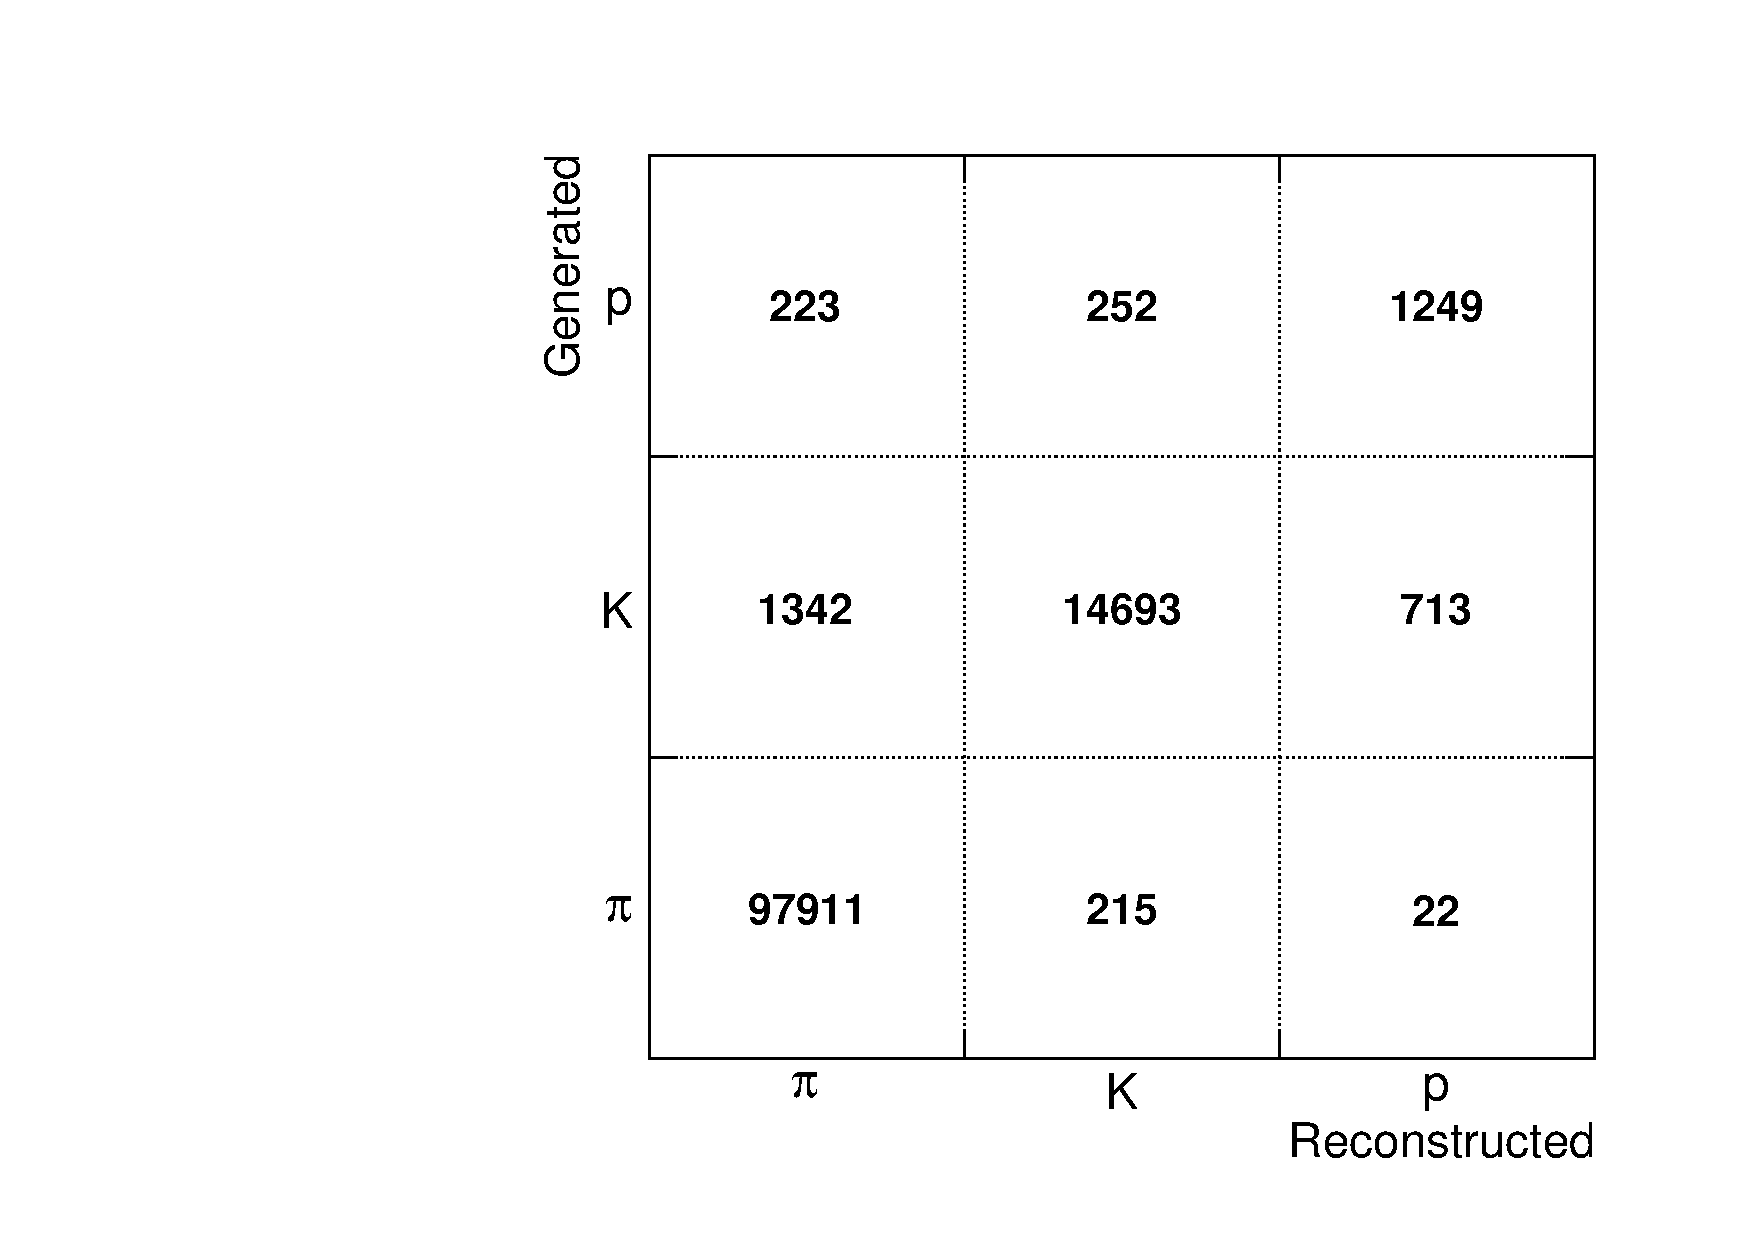
\includegraphics[width=0.45\textwidth]{ILD/plots/dedx-results.pdf}
    \caption{\sl Correlation histogram between generated particle type and reconstructed particle type produced by the cut-based PID algorithm.
    }
    \label{fig:dEdxResults_3}
  }
 
\end{figure}


Given the reconstruction purity illustrated in Fig.~\ref{fig:dEdxResults_3}, one concludes that the reconstructed charged kaons from the reconstructed vertices provide a reliable information on the charge of the initial b-hadron or b-quark. 

%%%%%%%%%%%%%%%%%%%%%%%%%%%%%%%%%%%%%%%%%%%
%%%%%%%%%%%%%%%%%%%%%%%%%%%%%%%%%%%%%%%%%%%
%%%%%%%%%%%%%%%%%%%%%%%%%%%%%%%%%%%%%%%%%%%
\subsection{Summary}
In this thesis, two basic b-quark charge signatures are used: 
\begin{itemize}
	\item \textit{Vertex charge}, which is computed as a sum of the reconstructed secondary and tertiary particle charges;
	\item\textit{ Kaon charge} - the charge of a kaon from the reconstructed secondary and tertiary vertices. 
\end{itemize}
The impurity of the vertex charge is caused by missing particles - particles, that were not assigned to the corresponding reconstructed vertices. 
Major reasons behind the missing particles are the following:
\begin{itemize}
	\item Charged track is not reconstructed;
	\item No assigned hits from VXD or FTD detectors, therefore the particle offset is not significant;
	\item Particle Flow Object is not reconstructed;
	\item Low generated offset.
\end{itemize}
A large inefficiency of the vertex reconstruction algorithm in forward region of ILD is observed.

The developed Vertex Charge Recovery algorithm assigns the missing particles to the reconstructed vertices using reconstructed observables. It increases the overall vertex charge purity by 7\% and the algorithm equalizes the vertex charge purity in the barrel region of the ILD detector. 

The kaons are identified using the dE/dx information from the TPC tracks. The developed angular correction makes dE/dx independent from the polar angle of the reconstructed track. Therefore, it increases the purity and efficiency of the kaon identification algorithms. 



%%%%%%%%%%%%%%%%%%%%%%%%%%%%%%%%%%%%%%%%%%%
%%%%%%%%%%%%%%%%%%%%%%%%%%%%%%%%%%%%%%%%%%%
%%%%%%%%%%%%%%%%%%%%%%%%%%%%%%%%%%%%%%%%%%%
\newpage
\section{Top quark production at the ILC}
\label{sec:TopProduction}
%Direct electroweak production of the top quark pairs
This section of the thesis describes an application of the b-quark charge measurement technique, described in Sec.~\ref{sec:JetChargeReconstruction}, to the polar angle measurement for the $e^+e^- \to t\bar{t}$ process at the ILC.%, which is used to determine the electroweak couplings of the top quark.
The end goal of this study is to increase efficiency of the b-quark polar angle reconstruction as comparing to the previous studies~\cite{bib:ILCTOP}.

The studies in this section have the following steps:
\begin{itemize}
	\item The setup of the study and the \ttbar\ event reconstruction provided in Sections~\ref{sec:TopProp}-\ref{sec:TopBkg};
	\item The description of the top quark charge information sources is given in Sec.~\ref{sec:ChargeOverview};
	\item The application of the b-quark charge combination as a proof of concept is in Sec.~\ref{sec:TopBCharge};
	\item The final combination of all top quark charge information and the final results are described in Sec.~\ref{sec:TopJetChargeCombo}.
\end{itemize}
%The measurements of the top quark properties is one of the key points of the \sm\ physics program at the ILC.

\subsection{Properties of the top quark}
\label{sec:TopProp}
The top quark is the heaviest elementary particle in the \sm\ with measured mass of around 173\,GeV~\cite{bib:TopMass}. This implies a very short lifetime of approximately 5$\cdot10^{-25}$\,s.
The top quark lifetime is short compared to a time needed for hadronization process  (10$^{-23}$\,s). Therefore, the top quark decays too fast to form hadrons. 
This fact permits to study the bare quark properties, like spin, via the quark decay particles. 

The dominant decay mode of the top quark is $t\to bW^+$, which is 99.8\% of all top decays in the \sm. The $W^\pm$ boson decays either into a lepton-neutrino pair or into a pair of quarks. The top quark decays thus leads to a six fermion final state of the $e^+e^-\to t\bar{t}$ process.
The $t\bar{t}$  decays are classified by the $W^\pm$ decay modes:
\begin{itemize}
	\item Fully hadronic decay $t\bar{t} \to bq\bar{q} \bar{b} q\bar{q}$ -  46.2\% of branching ratio;
	\item Semileptonic decay $t\bar{t} \to bq\bar{q} \bar{b} l\nu_l$ - 43.5\% of branching ratio;
	\item Fully leptonic decay $t\bar{t} \to b l^- \nu_{l^-} \bar{b} l^+\nu_{l^+}$ - 10.3\% of branching ratio.	
\end{itemize}


At the ILC it is possible to reconstruct and study all decay modes of the $t\bar{t}$ pair with a high selection efficiency.
%%%%%%%%%%%%%%%%%%%%%%%%%%%%%%%%%%%%%%%%%%%%%%%%%%%%%%%%%
%%%%%%%%%%%%%%%%%%%%%%%%%%%%%%%%%%%%%%%%%%%%%%%%%%%%%%%%%
%%%%%%%%%%%%%%%%%%%%%%%%%%%%%%%%%%%%%%%%%%%%%%%%%%%%%%%%%
\subsection{Setup of the study}
%The top quark pairs at the ILC can be produced at $\sqrt{s}=350$\,GeV and 500\,GeV. 
In this section of the thesis, the semileptonic $t\bar{t}$ pairs produced at $\sqrt{s}=500$\,GeV in the left-handed beam configuration are studied using full ILD simulation.
The total integrated luminosity used correspond to the 330\ifb.
%The integrated luminosity used is 150\ifb\ for the ideal beam polarization and 250\ifb for realistic beam polarization. The number of the generated events is 102255.
The top quark polar angle in the right-handed beam configuration was  successfully reconstructed in \cite{bib:Doublet}\cite{bib:ILCTOP}.
Therefore, this thesis concentrates on the left-handed beam configuration only, where one has inefficiency of the top polar angle reconstruction due to the event migration effect, as it was found in~\cite{bib:Doublet}~\cite{bib:Jeremy}.
The chosen center-of-mass energy allows for top pair production free from $t\bar{t}$ threshold QCD effects.
The cross sections at the Born level of the signal process $e^+e^- \to t\bar{t}$ and the major \sm\ background processes at the $\sqrt{s} = 500$\,GeV are summarized in Table~\ref{table:ttbarsigma}.

The clear process signature of two b-jets, two light jets from $W^\pm$ boson and an isolated lepton makes the semileptonic decay mode easily reconstructable and usable for the forward-backward asymmetry $A_{FB}$ measurement. 
An example of a \ttbar\ event in the ILD environment is shown in Fig.~\ref{fig:TopEvent_3}.

\begin{figure}
	{\centering
		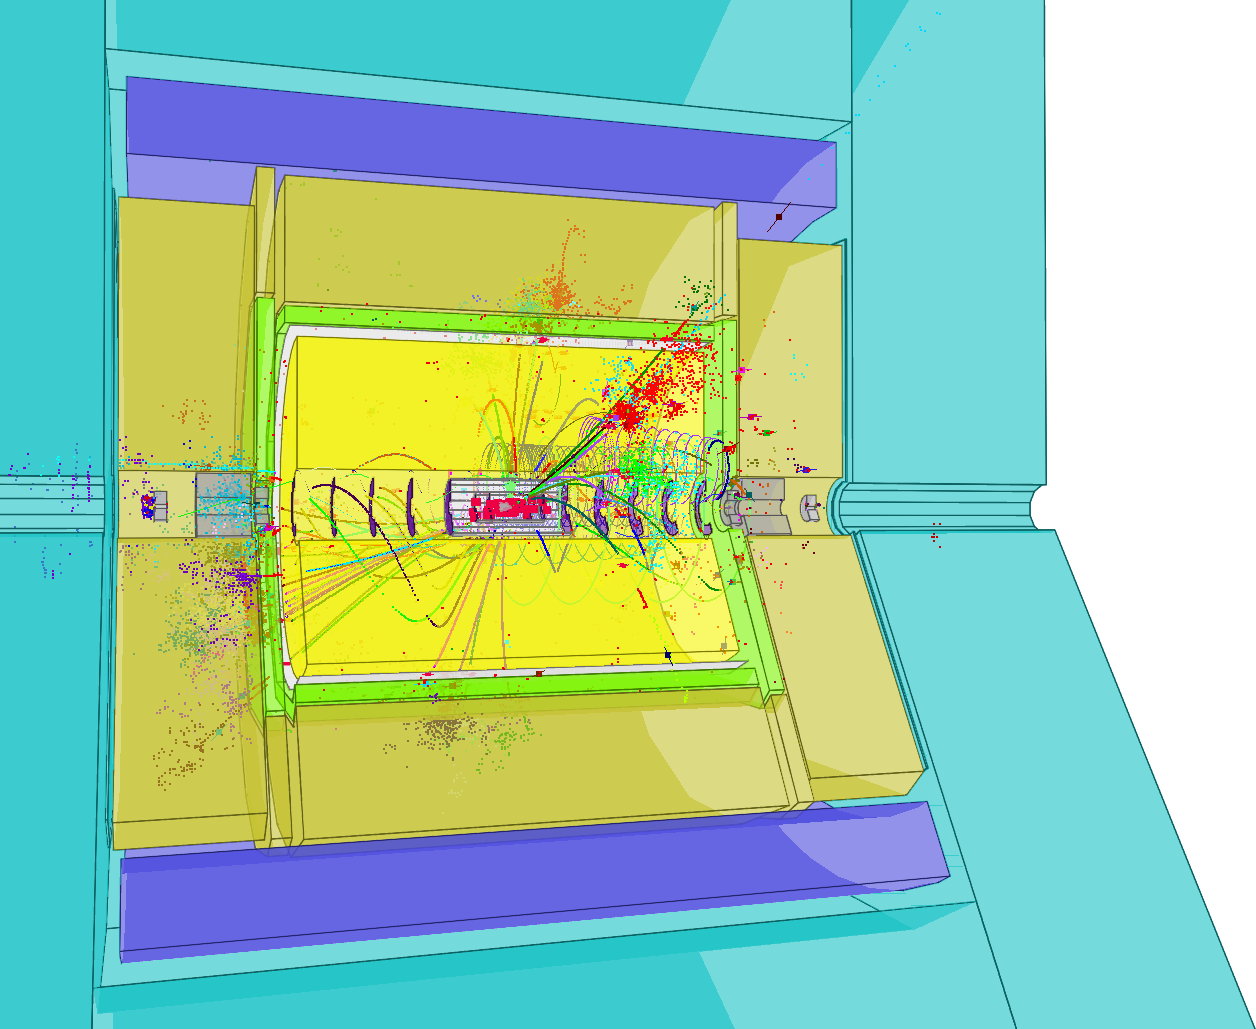
\includegraphics[clip, trim=0.cm 0cm 7.9cm 0cm, width=0.55\textwidth]{ILD/graphics/ild-ttbar.png}
		\caption{\sl Event display of the \ttbar\ pair production process in the ILD simulation.
		}
		\label{fig:TopEvent_3}
	}
	
\end{figure}
%This choice is motivated to use the b-quark charge measurement to overcome the $W^\pm$ lepton migration effect, described in~\cite{bib:ILCTOP}, it also allows for a direct comparison and combination of the new results with previous studies done using $W^\pm$ lepton charge method.

%This chapter concentrates only on the left-handed electron polarization case, because of the lepton migration problem caused by the $W^\pm$ kinematics. 
%The previous studies found  
The main goal of the study is to extend studies~\cite{bib:ILCTOP}~\cite{bib:Jeremy} by a new b-quark charge measurement techniques, which should bring down the statistical uncertainties on the \ttbar Z$^0$ form factors and couplings.  

%\subsection{Top quark decay modes}

\subsection{Top quark reconstruction}\label{sec:TopRec}
In this thesis, the top reconstruction method, which was developed for~\cite{bib:ILCTOP} is applied. It has the following steps:
\begin{itemize}
	\item Isolated lepton identification is done with the LAL LeptonFinder algorithm~\cite{bib:Doublet}, which is designed to find an energetic lepton or a lepton, which has a significant transverse momentum with respect to the neighbored jets. 
	\item The events, after excluding the isolated lepton, are clustered into four jets by the Durham jet clustering algorithm.
	\item The b-jet tagging done by LCFI+ is used to identify the two b-jets and sorted by btag value for the background rejection cuts. 
	\item The last step of the top quark reconstruction is to associate one of the b-jets with the two light jets from the hadronic $W^\pm$ decay.  One has two possibilities to combine the jets and one chooses the best combination by minimizing the following expression:
	\begin{equation}
	\label{formula:Chi2Top_3}
	d^2_{t} = (\frac{m_{cand}-m_{t}}{\sigma_{m_t}})^2 + (\frac{E_{cand}-E_{beam}}{\sigma_{E_{beam}}})^2+(\frac{p^*_b-68\,GeV}{\sigma_{p^*_b}})^2 + (\frac{\cos\theta_{bW}-0.23}{\sigma_{\cos\theta_{bW}}})^2,
	\end{equation}
	where $m_{cand}$ and $E_{cand}$ are the invariant mass and the energy of the top quark candidate, $m_t$ and $E_{beam}$ are the input top quark mass and the nominal beam energy of 250\,GeV, $p^*_b$ is the momentum of the b quarks in the top quark rest frame with nominal value of 68\,GeV and $\cos\theta_{bW}$ is the angle between the b quark and the $W^\pm$ boson with a nominal value of 0.23.
	\item The neutrino from leptonic $W^\pm$ boson decay is reconstructed using the recoil momentum method. The reconstructed neutrino is used to calculate the leptonic $W^\pm$ boson mass and leptonic top quark mass. 
\end{itemize}

The reconstructed distributions of the top quark and $W^\pm$ boson invariant masses are shown in Fig.~\ref{fig:TopWmass_3}. The values of the reconstructed peaks indicate the correct reconstruction flow. 

\begin{figure}[h]
	{\centering
		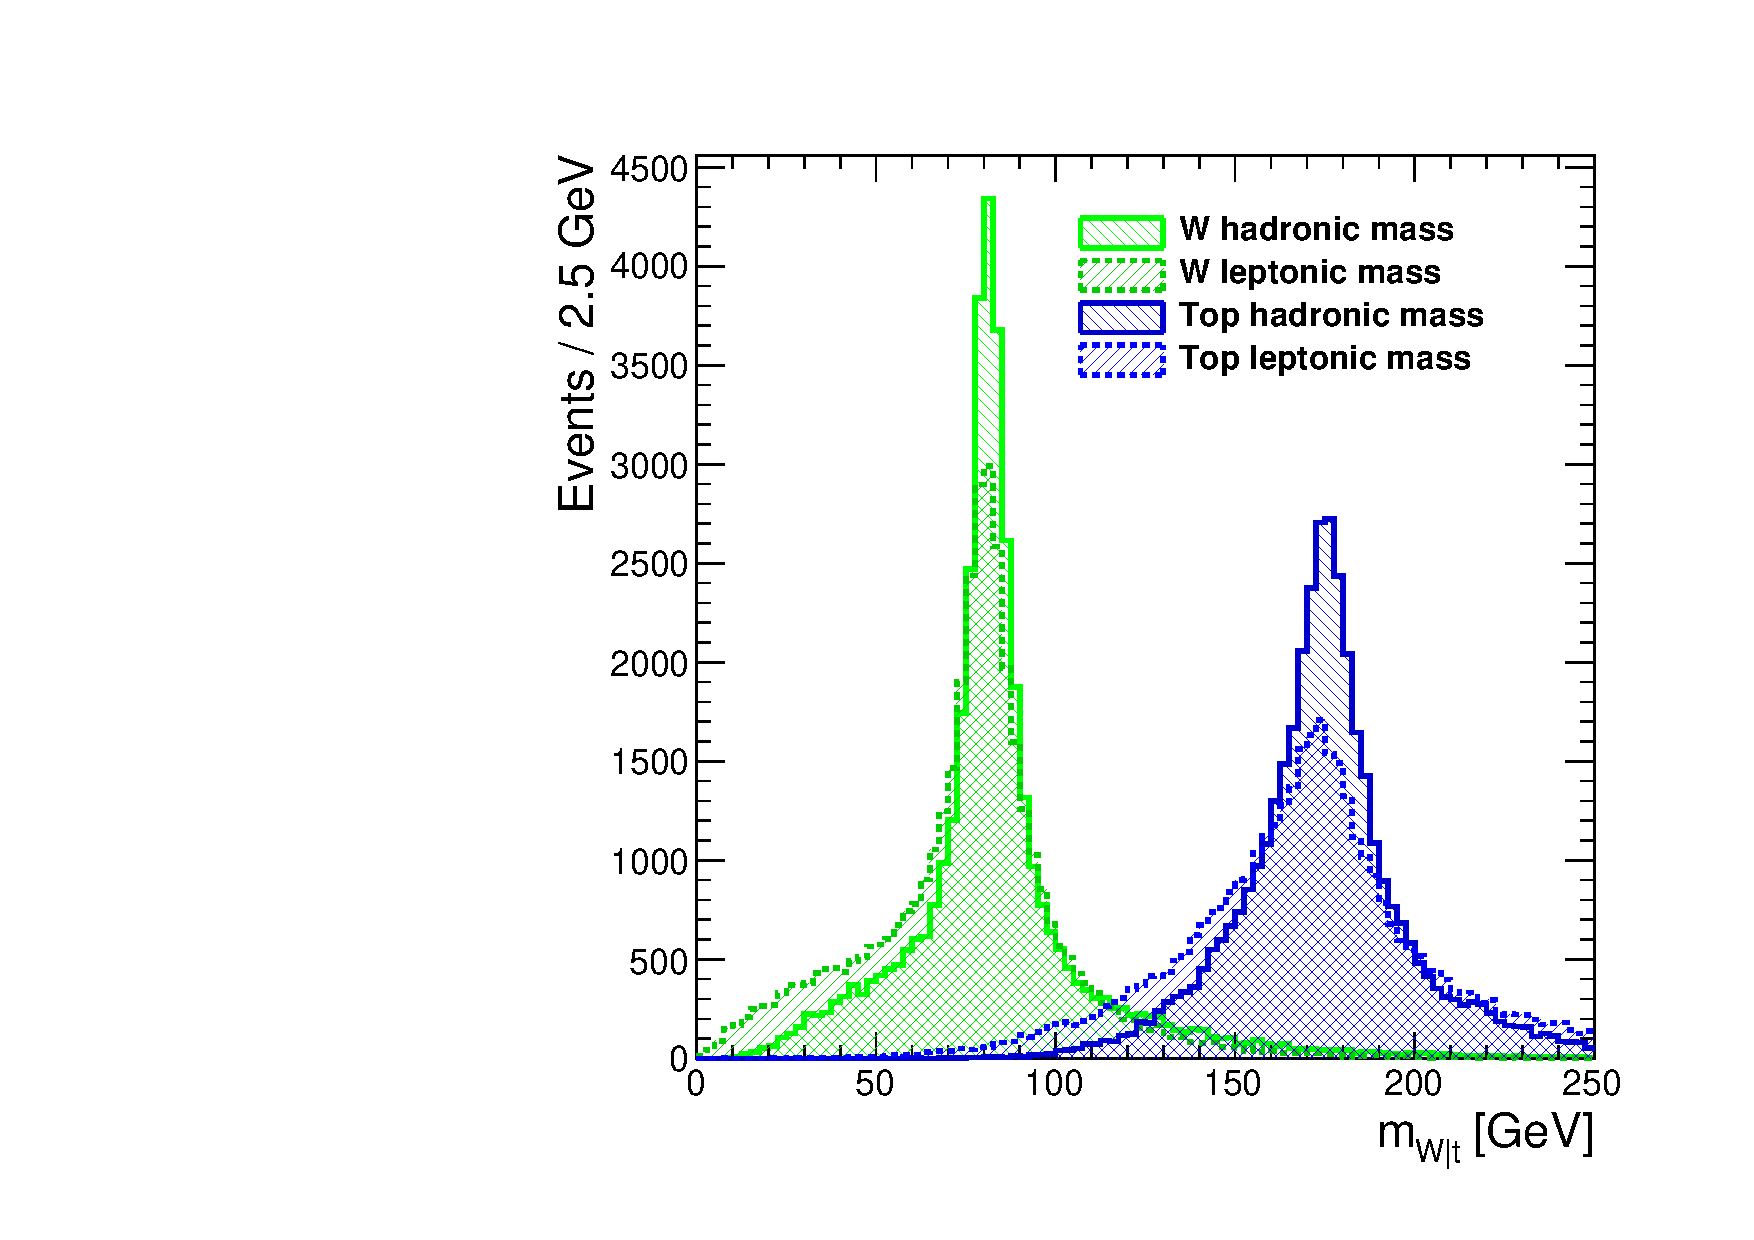
\includegraphics[width=0.55\textwidth]{ILD/plots/top-w-mass-new.pdf}
		\caption{\sl Reconstructed invariant mass distributions of the hadronic top quark and hadronic $W^\pm$ boson decays.
		}
		\label{fig:TopWmass_3}
	}
	
\end{figure}

The $W^\pm$ boson kinematics and that of the b-quark in the \ttbar\ process depends strongly on the polarization of the initial state:
\begin{itemize}
	\item In case of a right-handed electron beam the events are enriched with right-handed top quarks. Due to the structure of the weak interaction, top quark decays into an energetic $W^\pm$ boson, which is emitted into top quark direction, and a relatively soft b-quark;
	\item In case of a left-handed electron beam the sample is enriched with the left-handed top quarks, which decay into soft $W^\pm$ bosons and energetic b-quarks, which are predominantly aligned with the top quark direction. 
\end{itemize}
An incorrect assignment of b-jet and $W^\pm$ jets compromises the top quark charge reconstruction needed for the top polar angle measurement. 

\subsection{Background processes}\label{sec:TopBkg}
The main background processes are summarized in Table~\ref{table:ttbarsigma}. 
The previous studies~\cite{bib:ILCTOP}\cite{bib:Doublet} have shown that the major backgrounds to the semileptonic \ttbar\ decay are the single top process and fully hadronic or fully leptonic \ttbar\ decays. 
%Several \sm\ processes give a rise to the six fermion final state, 
        \begin{table}[H]
        \begin{center}
        \begin{tabular}{l c c c}
        \hline
	Channel & $\sigma_{unpol.}$\ [fb] & $\sigma_{LR}$ [fb] &  $\sigma_{LR}$ [fb] \\
	\hline
	$t\bar{t}$ & 572 & 1564 & 724 \\
	$\mu\mu$ & 456 & 969 & 854 \\
	$uu + cc + ss + dd$ & 2208 & 6032 & 2793 \\
	$b\bar{b}$ & 372 & 1212 & 276 \\
	$\gamma Z^0$ & 11185 & 25500 & 19126 \\
	$WW$ & 6603 & 26000 & 150 \\ 
	$Z^0Z^0$ & 422 & 1106 & 582 \\
	$Z^0WW$ & 40 & 151 & 8.7 \\
	$Z^0 Z^0 Z^0$ & 1.1 & 3.2 & 1.22 \\
        \hline
        \end{tabular}
        \end{center}
        \caption{\sl Unpolarized and 100\% polarized cross sections at the Born level for signal and background processes at $\sqrt{s}=500$\,GeV~\cite{bib:ILCTOP}. }
        \label{table:ttbarsigma}
        \end{table}


One uses the kinematical cuts to suppress the background processes, which were originally developed in ~\cite{bib:Doublet}~\cite{bib:Jeremy} and defined in Table~\ref{table:ttbarselection}
        \begin{table}[H]
        \begin{center}
        \begin{tabular}{l c c c}
        \hline
	Selection criteria & \ttbar\ semileptonic  & WW semileptonic &  \bbbar  \\
	\hline
%	Initial numbers & 102255 (100\%) & 1654657 (100\%) & 179520 (100\%) \\
	Isolated lepton 						& 67\% & 59.6\% & 9.5\% \\
	btag$_1$ $>$ 0.8 or btag$_2$ $>$ 0.3 	& 61\% & 1.22\% & 7.3\% \\
	Thrust $<$ 0.9 							& 60.5\% & 0.19\% & 1.\% \\
	Hadronic mass 							& 59.4\% & 0.087\% & 0.3\% \\
	Reconstructed $m_W$ and $m_t$ 			& 54.4\% & 0.04\% & 0.15\% \\
		\hline
	Relative cross section 					& 1 & 5.0 & 1.9 \\
        \hline
        \end{tabular}
        \end{center}
        \caption{\sl Efficiency of signal and non-\ttbar\ backgrounds after different cuts for left-handed beam polarization. Background values are taken from~\cite{bib:Jeremy}.}
        \label{table:ttbarselection}
        \end{table}

The previous studies demonstrated, that the purity of the full semileptonic \ttbar\ process selection is 91\% and final event selection efficiency is 54\%~\cite{bib:ILCTOP}.
The residual background is homogeneously distributed in $\cos\theta$, as it is shown in Fig.~\ref{fig:ILCTOPAFB}, which allows to concentrate the present studies on the signal process only. 

%%%%%%%%%%%%%%%%%%%%%%%%%%%%%%%%%%%%%%%%%%%%%%%%%%%%%%%
%%%%%%%%%%%%%%%%%%%%%%%%%%%%%%%%%%%%%%%%%%%%%%%%%%%%%%%
%%%%%%%%%%%%%%%%%%%%%%%%%%%%%%%%%%%%%%%%%%%%%%%%%%%%%%%
\subsection{Results}

In this study, the top polar angle is calculated by using the reconstructed top or anti-top quark, which decayed hadronically.
In case of the reconstructed $\bar{t}$ quark, the polar angle is changed from $\theta_{\bar{t}} \to \theta_{t} + \pi$, or $\cos\theta_{\bar{t}} \to -\cos\theta_{t}$. 
%Hence, the main challange of the study is to correctly identify the charge of the reconstructed hadronic top or anti-top quark. 

The charge of the reconstructed top quark in this study is derived from three basic signatures: b-quark charge measurement using the reconstructed secondary vertices or the vertex charge, the reconstructed kaon charge, and the $W^\pm$ lepton charge. 
The top quark polar angle, reconstructed with the three basic methods is demonstrated in Fig.~\ref{fig:OneCharge_3}.
All three methods show a disagreement between the reconstructed and generated distributions.
These deviations are a consequence of a significant charge impurity which leads to a confusion of a top quark with an anti-top quark.
%These charge migrations result in the divergence between the generated polar angle distribution and reconstructed curves for all three methods. 


\begin{figure}
	\centering
	\begin{subfigure}{0.33\textwidth}
		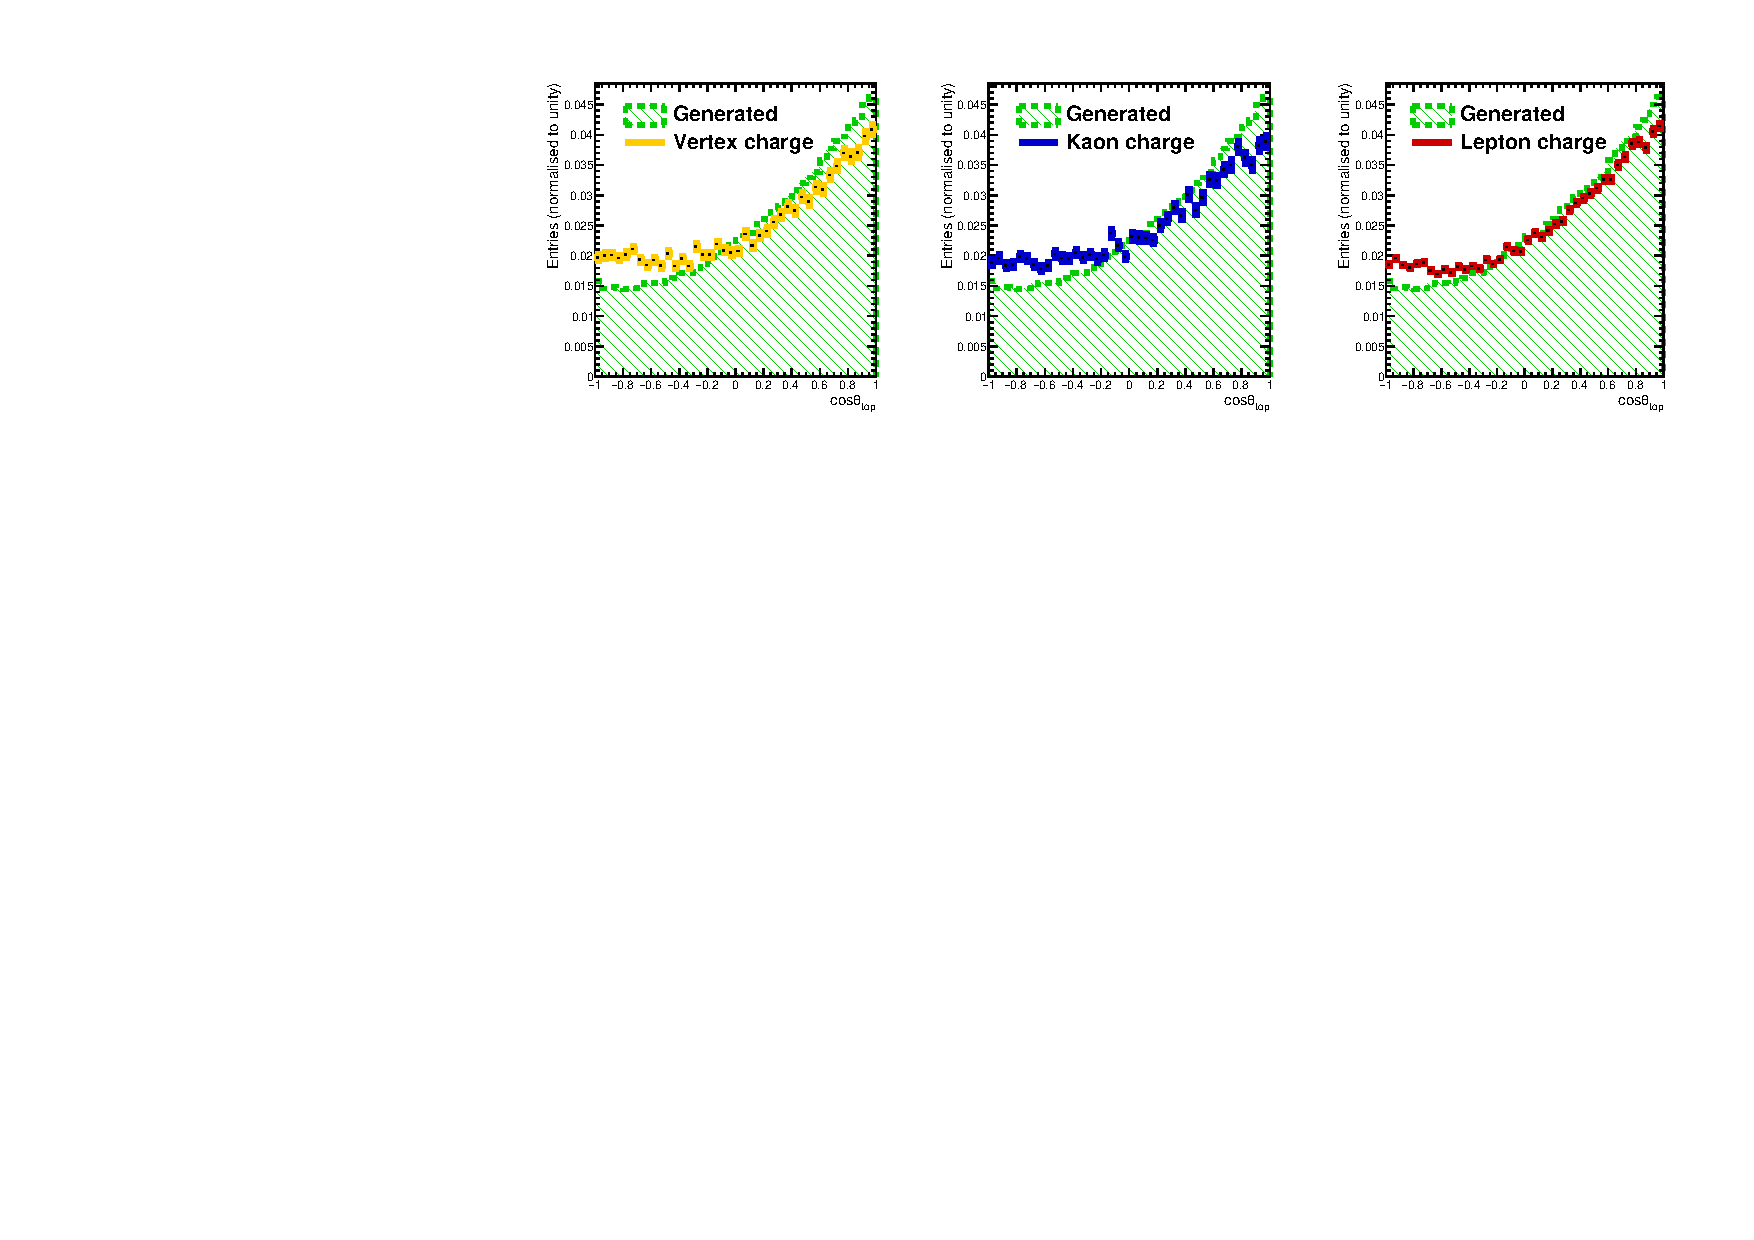
\includegraphics[clip, trim=0.1cm 0cm 13.9cm 0cm,width=0.99\textwidth]{ILD/plots/one-charge.pdf}
		\caption{\label{fig:OneCharge_a_3} }
	\end{subfigure}% 
	\begin{subfigure}{0.33\textwidth}
		\centering
		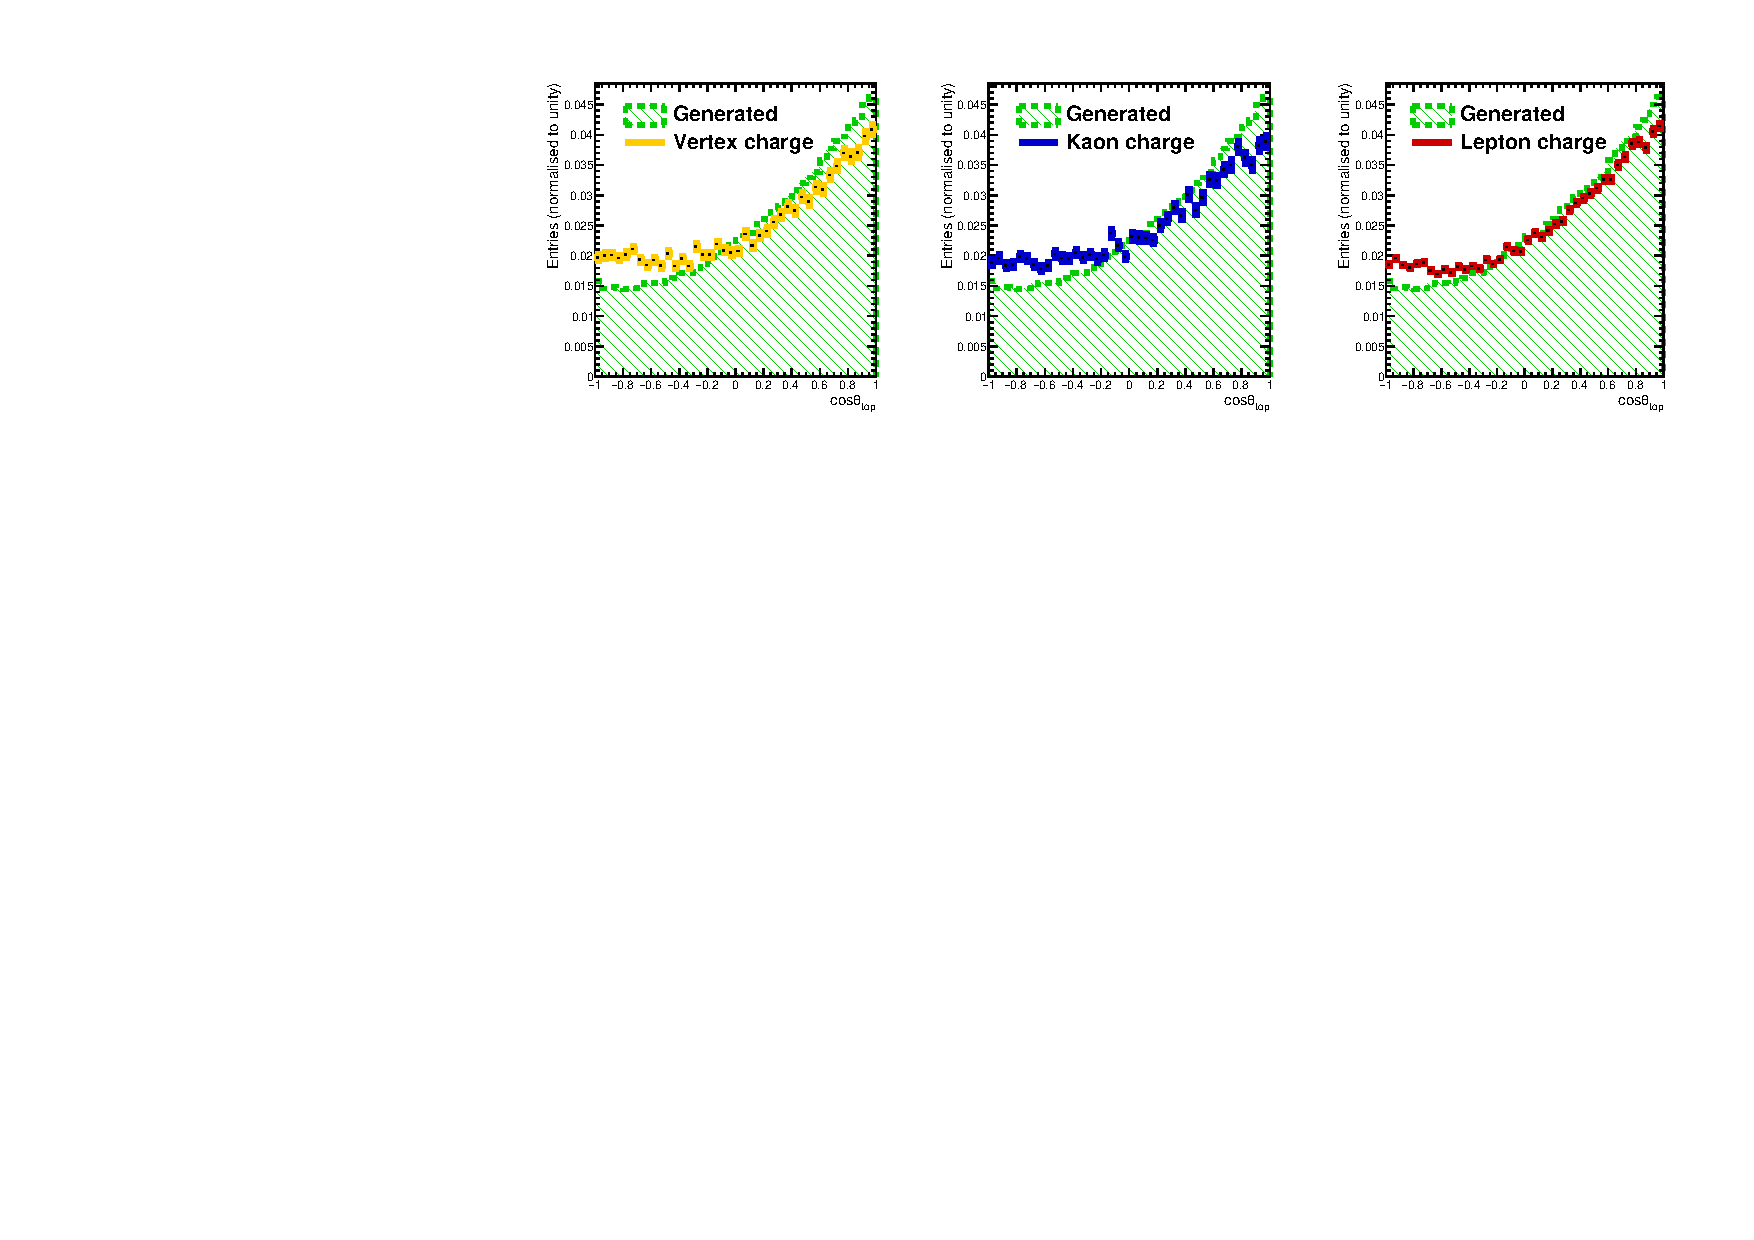
\includegraphics[clip, trim=6.78cm 0cm 7.3cm 0cm,width=0.99\textwidth]{ILD/plots/one-charge.pdf}
		\caption{\label{fig:OneCharge_b_3} }
	\end{subfigure}
	\begin{subfigure}{0.33\textwidth}
		\centering
		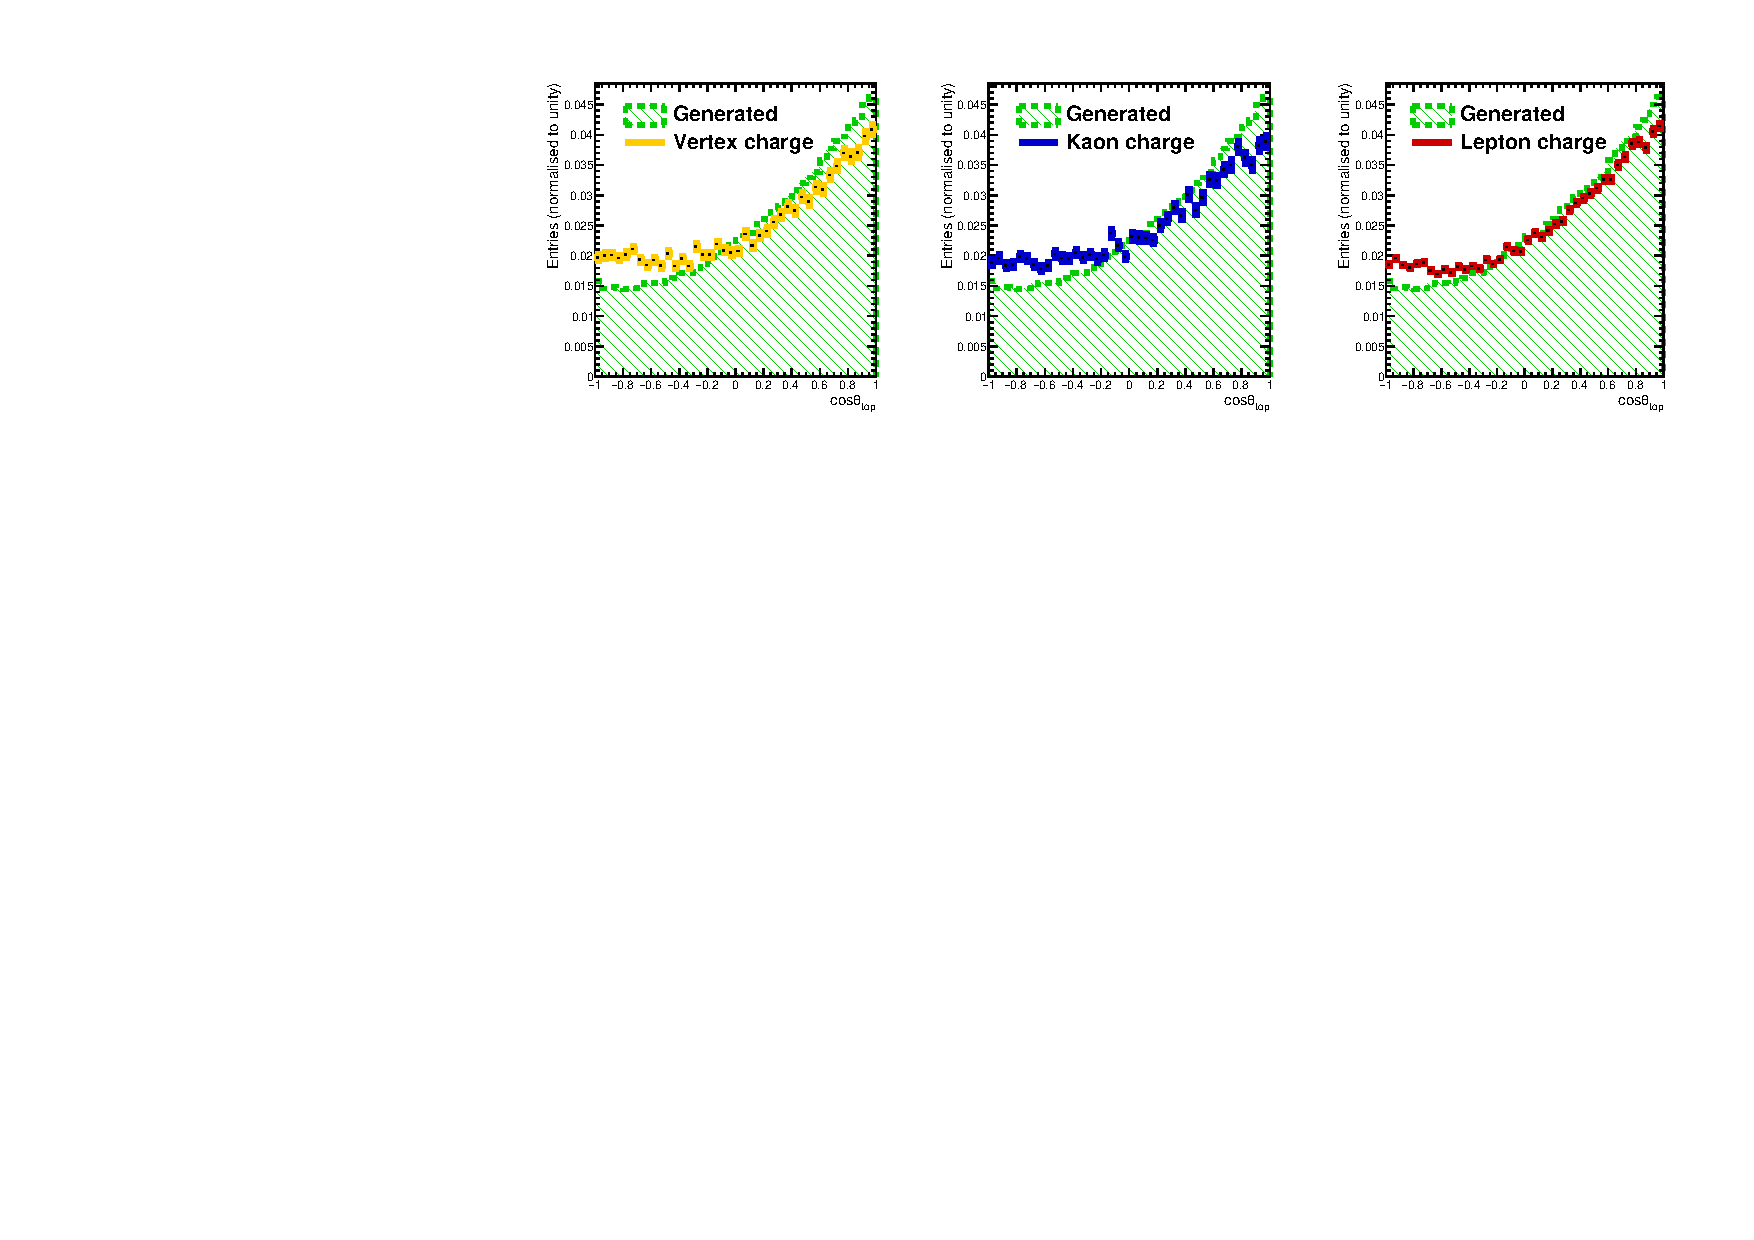
\includegraphics[clip, trim=13.6cm 0cm 0.4cm 0.cm,width=0.99\textwidth]{ILD/plots/one-charge.pdf}
		\caption{\label{fig:OneCharge_c_3} }
	\end{subfigure}
	\caption{\sl Generated polar angle distribution compared to reconstructed polar angle using standalone vertex charge (a), standalone kaon charge (b) and $W^\pm$ lepton charge(c). }
	
	\label{fig:OneCharge_3}
\end{figure}

In this studies, the quality of the top quark polar angle reconstruction is estimated by the ratio of the reconstructed forward-backward asymmetry $A_{FB}^{rec}$ over the generated $A^{gen}_{FB}$ values.
For the vertex and the kaon charge methods the $A_{FB}^{rec}/A^{gen}_{FB} \approx 63\%$, while for the $W^\pm$ lepton charge method is 74\% without any additional cuts. 
Hence, the standalone b-quark charges and $W^\pm$ lepton charge signatures are not reliable enough to compute the top quark polar angle and $A_{FB}$ precisely. 
%%%%%%%%%%%%%%%%%%%%%%%%%%%%%%%%%%%%%%%%%%%%%%%%%%%%%%%%%%%
%%%%%%%%%%%%%%%%%%%%%%%%%%%%%%%%%%%%%%%%%%%%%%%%%%%%%%%%%%%
%%%%%%%%%%%%%%%%%%%%%%%%%%%%%%%%%%%%%%%%%%%%%%%%%%%%%%%%%%%
\subsubsection{Charge combination}\label{sec:ChargeOverview}

To decrease this charge impurity, one uses the compatible combinations of two or more charge signatures.
In a semileptonic \ttbar\ event one has two b-jets with vertex and kaon charge signatures each and one $W^\pm$ lepton charge signature. 
%The general charge combination rules are:
One has the following charge combination rules to accept an event for the top quark polar angle measurement:
\begin{itemize}
	\item Two b-jets should have opposite vertex and kaon charges;
	\item The kaon and vertex charge should have the same sign within one b-jet;
	\item The $W^\pm$ lepton charge should be opposite to the b-quark charges within one reconstructed top or anti-top quark decayed leptonically; 
	\item The  $W^\pm$ lepton charge should have the same charge as the b-quark charge from the top quark decayed hadronically.
	\item The $W^\pm$ lepton charge can be used standalone after a cut on the reconstructed top quality.
\end{itemize}

According to these rules, one has the following charge pair signatures for a semileptonic \ttbar\ event:
\begin{itemize}
	\item Vertex charge from one b-jet in combination with vertex charge from another b-jet, abbreviated as {\sc vtx+vtx};
	\item Kaon charge from one b-jet in combination with kaon charge from another b-jet ({\sc kaon+kaon});
	\item Vertex charge and kaon charge combination from the same b-jet ({\sc vtx+kaon});
	\item Vertex charge and kaon charge combination from different b-jets ({\sc vtx+kaon'});
	\item Vertex charge from a b-jet  in combination with $W^\pm$ lepton charge ({\sc l+vtx});
	\item Kaon charge from a b-jet in combination with $W^\pm$ lepton charge ({\sc l+kaon});
	\item $W^\pm$ lepton charge after cuts on the reconstructed top quality. ({\sc l }cut).
\end{itemize}
Multiple reconstructed charge pair signatures are possible within one event.

%%%%%%%%%%%%%%%%%%%%%%%%%%%%%%%%%%%%%%%%%%%%%%%%%%%%%%%%%%%
%%%%%%%%%%%%%%%%%%%%%%%%%%%%%%%%%%%%%%%%%%%%%%%%%%%%%%%%%%%
%%%%%%%%%%%%%%%%%%%%%%%%%%%%%%%%%%%%%%%%%%%%%%%%%%%%%%%%%%%
\subsubsection{Standalone b-quark charge application}\label{sec:TopBCharge}
In this section, the concept of the b-quark charge measurement is validated by determining the top quark polar angle solely from the vertex and the kaon charges. 
%In this section, to prove the concept of the b-quark charge measurement, only the vertex charge and kaon charge combinations are used to compute the top polar angle. 
In case of the left-handed electron beam, the b-quarks are emitted into the direction of the initial top quark, which makes possible the standalone application of the b-quark charge measurement. 

The vertex charge and kaon charge methods were used to compute top polar angle distribution shown in Fig.~\ref{fig:TopAsymmetryNoCutBjet_3}, where one sees a good agreement between the generated and reconstructed top polar angle histograms. 
The b-quark charge measurement shows a good precision on the asymmetry $A_{FB}^{rec}/A^{gen}_{FB} \approx 93\%$ with the total efficiency of 16\%.

\begin{figure}
	\centering
	\begin{subfigure}{0.5\textwidth}
		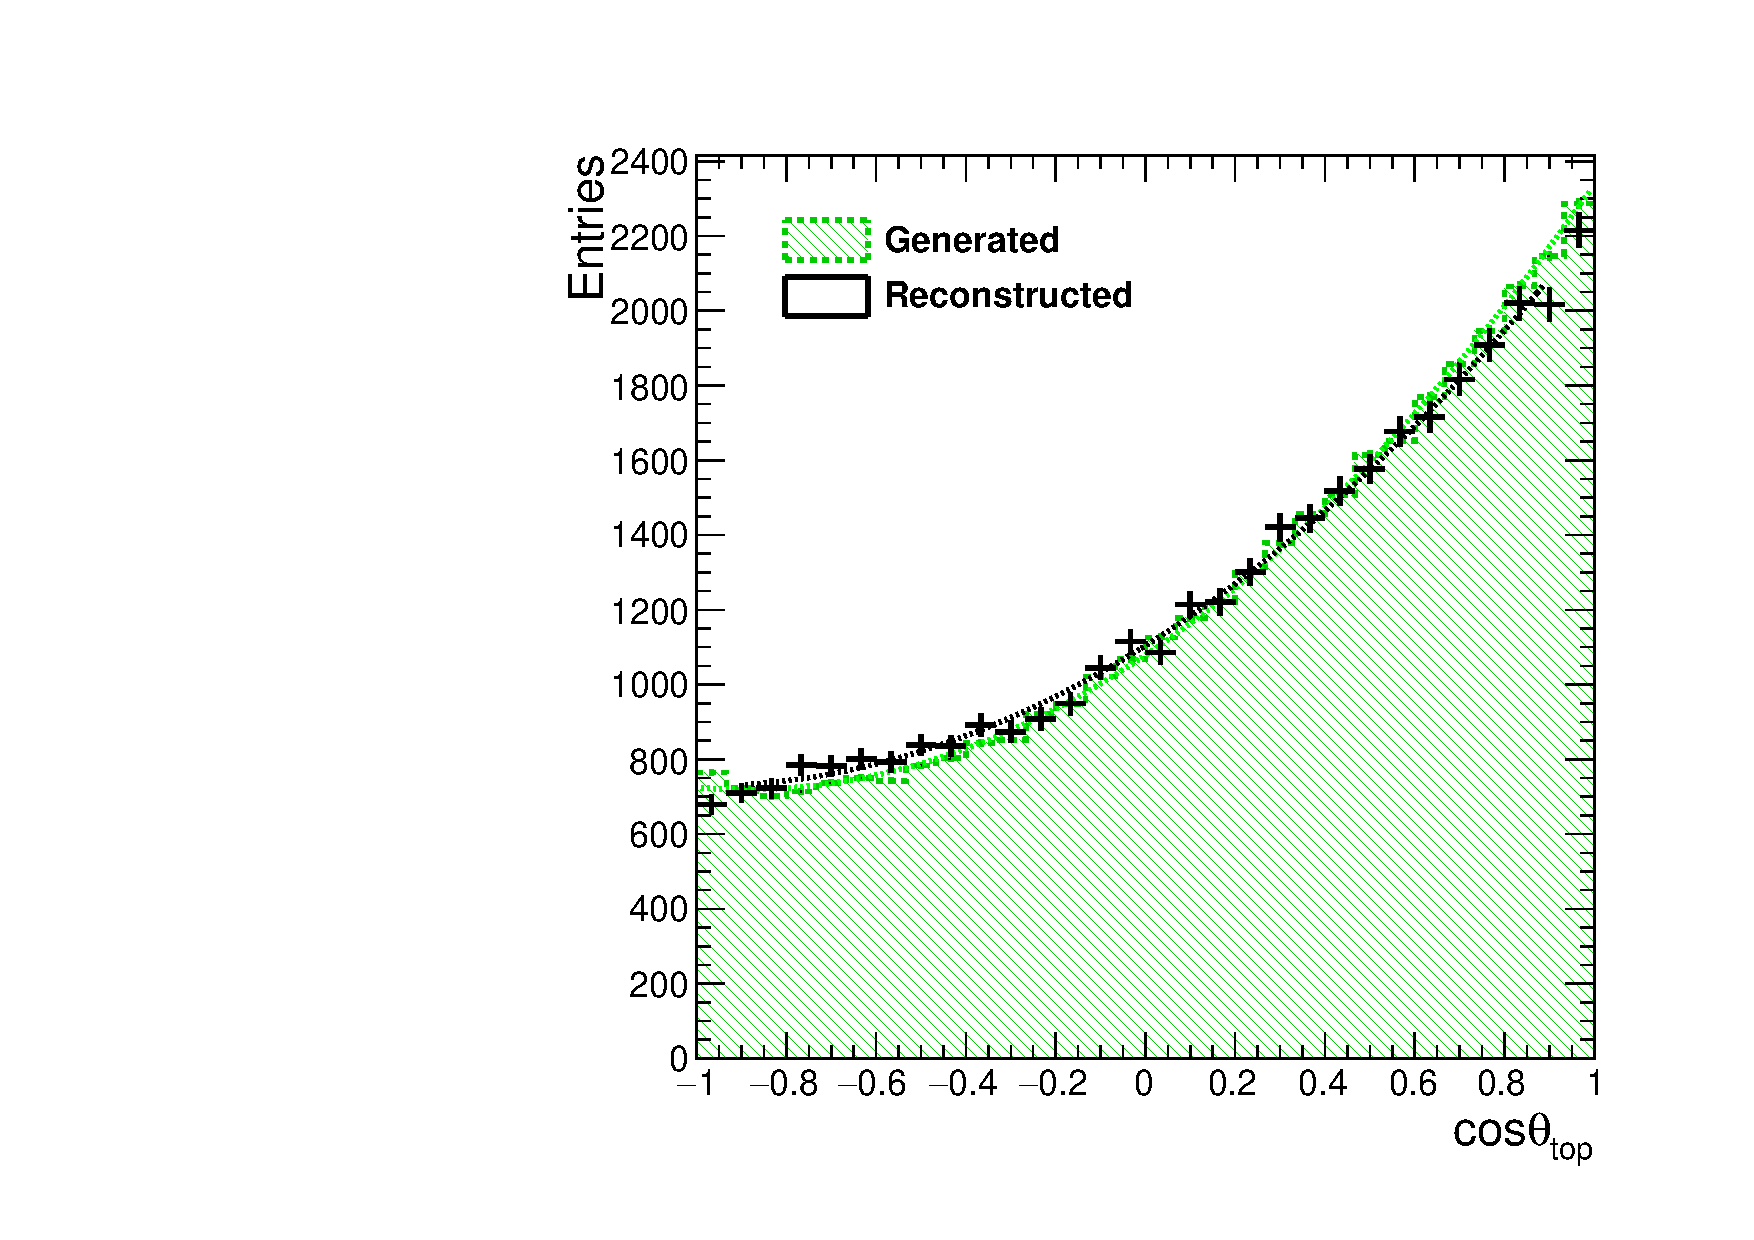
\includegraphics[width=0.95\textwidth]{ILD/plots/top-asymmetry-bonly-gcut.pdf}
		\caption{\label{fig:TopAsymmetryNoCutBjet_a_3} }
	\end{subfigure}% 
	\begin{subfigure}{0.5\textwidth}
		\centering
		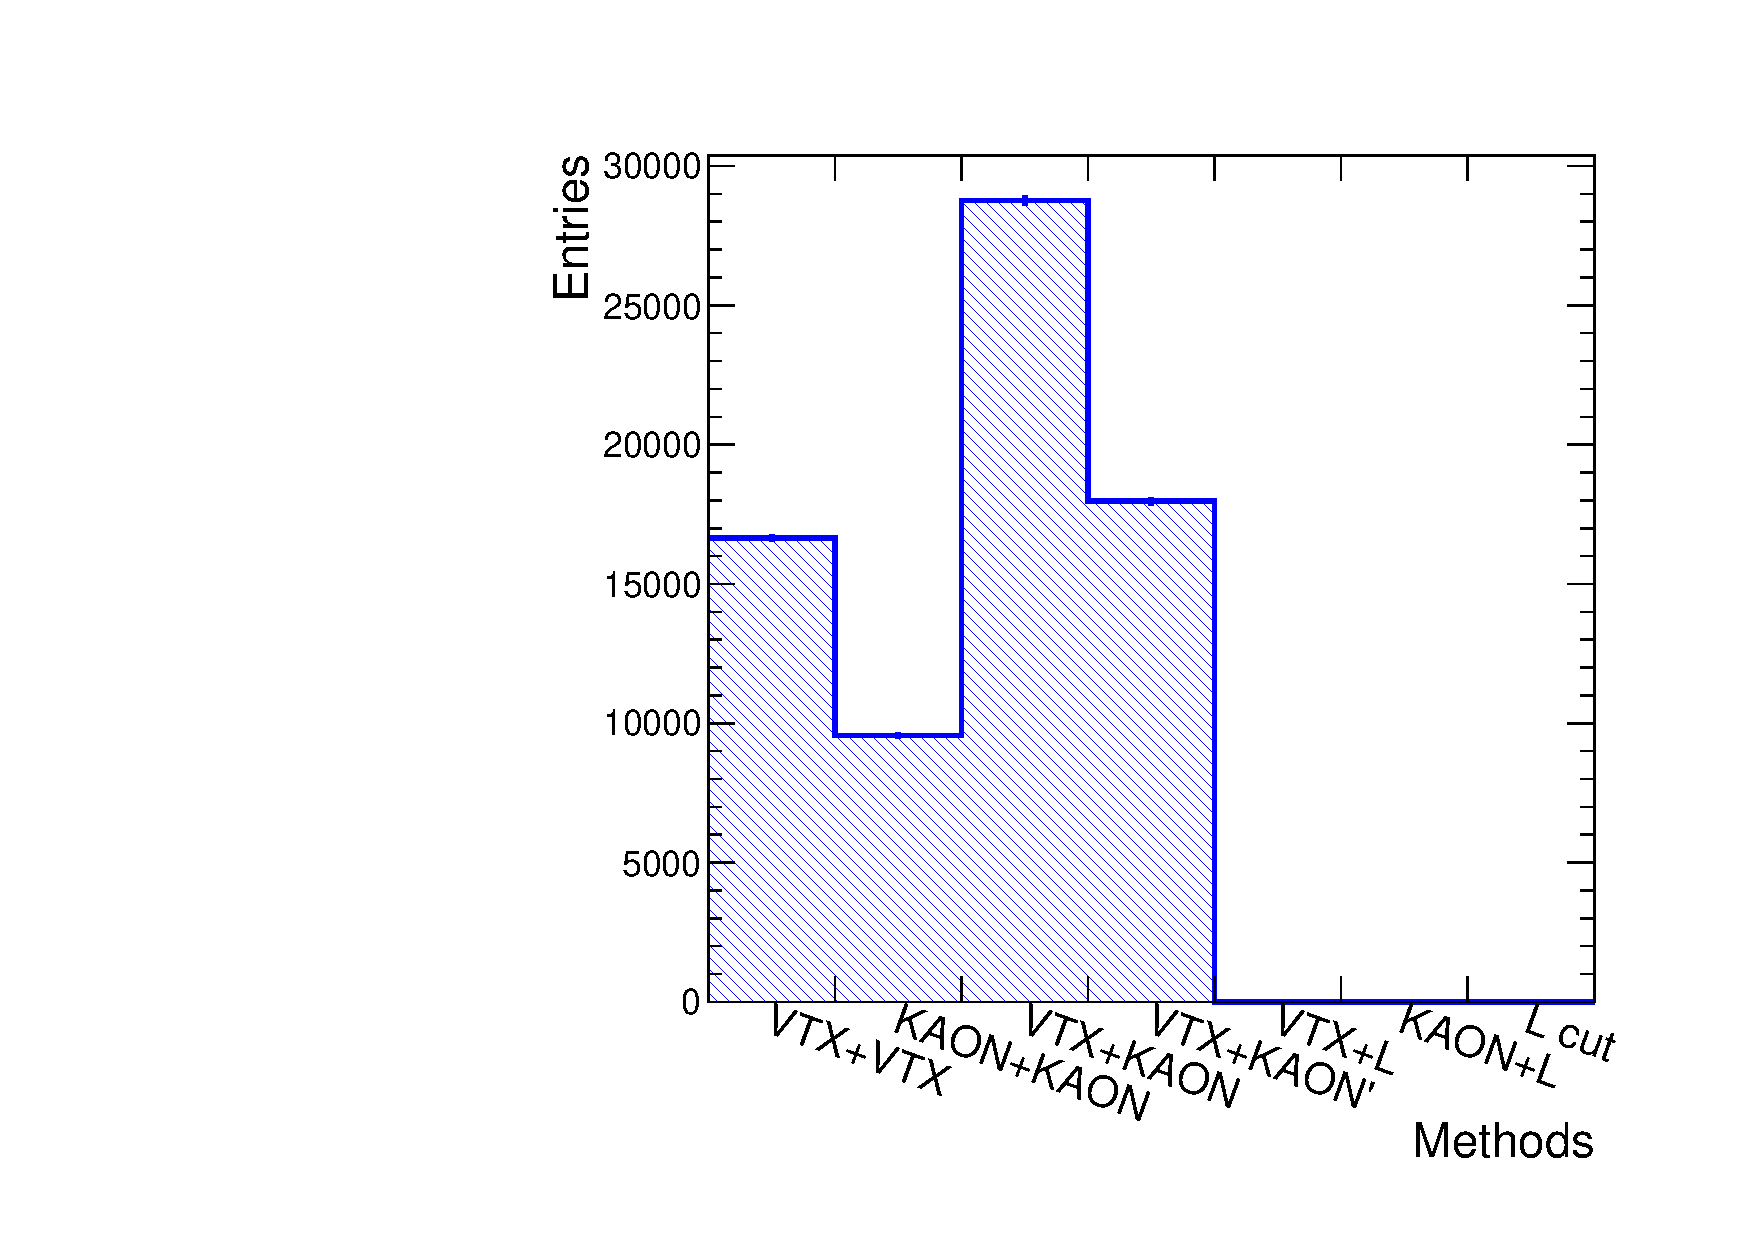
\includegraphics[width=0.95\textwidth]{ILD/plots/top-methods-bonly-gcut.pdf}
		\caption{\label{fig:TopAsymmetryNoCutBjet_b_3} }
	\end{subfigure}
	\caption{\sl Generated polar angle distribution compared to reconstructed polar angle using charge signature combinations from b-jets only. }
	\label{fig:TopAsymmetryNoCutBjet_3}
\end{figure}

The most used method is the vertex charge and kaon charge combination from the same b-jet, as can be seen from Fig.~\ref{fig:TopAsymmetryNoCutBjet_b_3}, which is due to the chosen asymmetric cuts on the b-tag values. 
Several charge combinations are possible for a single \ttbar\ event. 


\begin{figure}
	{\centering
		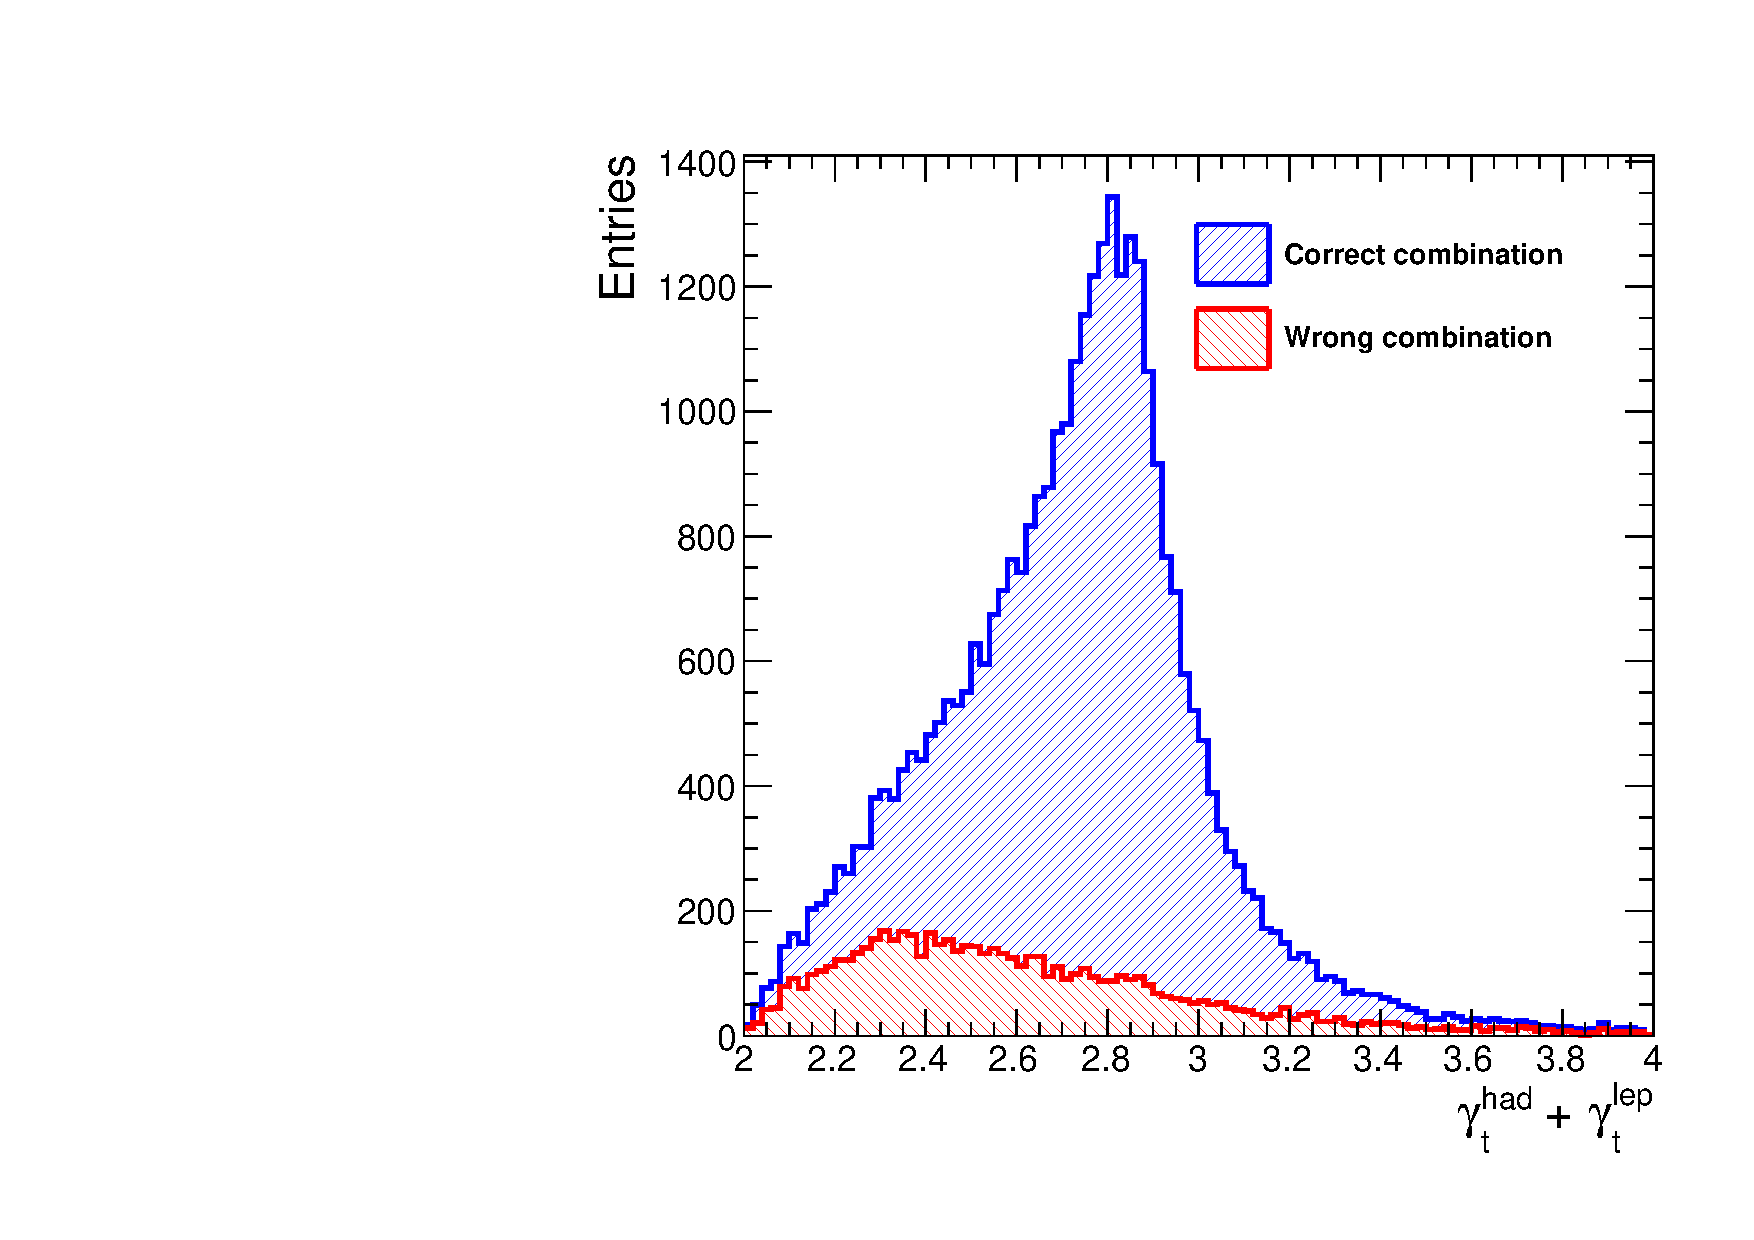
\includegraphics[width=0.55\textwidth]{ILD/plots/top-gamma.pdf}
		\caption{\sl Sum of the Lorentz gamma factors for leptonic and hadronic reconstructed tops separated into the wrongly and correctly reconstructed hadronic decay combinations.
		}
		\label{fig:TopGamma_3}
	}
	
\end{figure}

The sample in enriched by the good hadronic top quark combinations using the cut
\begin{equation}
 \gamma^{lep}_t + \gamma^{had}_t > 2.4,
\end{equation}
 as suggested by the histogram in Fig.~\ref{fig:TopGamma_3}, where Lorentz factor $\gamma_t = E_t / m_t$ depends on the reconstructed top quark energy $E_t$ and mass $m_t$.
To increase the vertex charge purity the following cuts are applied on the b-hadron kinematics in case of the vertex charge usage:
\begin{equation}
btag > 0.8\text{ and } |p|_{had} > 35\text{\,GeV}.
\end{equation}
One can use the purity distributions in Fig.~\ref{fig:RecoveryPurity_3} to optimize the cuts on the b-hadron kinematics. 
%One can purify the sample by changing the cuts on the b-hadron kinematics, but with a penalty on sample statistics. 

This result proves, that the  b-quark charge measurement can be used directly on the fully hadronic \ttbar\ decays for left-handed electron polarization, which will significantly increase the statistics needed for top coupling estimation. 

The vertex charge recovery increases the overall statistics by 7\% and the $A_{FB}^{rec}/A^{gen}_{FB}$ ratio by 4\%. 
However, the effects of the vertex charge recovery are much more essential for the $e^+e^-\to b\bar{b}$ process, discussed in Section~\ref{sec:BBBarresults}.

%%%%%%%%%%%%%%%%%%%%%%%%%%%%%%%%%%%%%%%%%%%%%%%%%%%%%%%%%%%
%%%%%%%%%%%%%%%%%%%%%%%%%%%%%%%%%%%%%%%%%%%%%%%%%%%%%%%%%%%
%%%%%%%%%%%%%%%%%%%%%%%%%%%%%%%%%%%%%%%%%%%%%%%%%%%%%%%%%%%
\subsubsection{B-quark charge and lepton charge combination}
\label{sec:TopJetChargeCombo}
The events with $W^\pm$ lepton charge migration can be efficiently rejected using  a cut on $\chi^2_{top}$~\cite{bib:Jeremy}, which is defined as:
\begin{equation}
	\label{formula:Chi2TopLepton_3}
	\chi^2_{top} = (\frac{\gamma_t^{had}-1.435}{\sigma_{\gamma_{t}}})^2 + (\frac{p^*_b-68}{\sigma_{\gamma_{p^*_b}}})^2 + (\frac{\cos\theta_{bW} - 0.23}{\sigma_{\cos\theta_{bW}}})^2,
\end{equation}
where $p^*_b$ and $\cos\theta_{bW}$ have been used in Eq.~\ref{formula:Chi2Top_3} and Lorentz factor $\gamma_t=E_{t}/m_{t}$ of the reconstructed top quark decayed hadronically. The $\chi^2_{top}$ is constructed to be minimal around the expectation values of the used variable distributions.
The distributions of the events with correctly assigned leptons and migrated leptons for all variables used in (\ref{formula:Chi2TopLepton_3}) are shown in Fig.~\ref{fig:TopChiVariables_3}.


\begin{figure}
	\centering
	\begin{subfigure}{0.33\textwidth}
		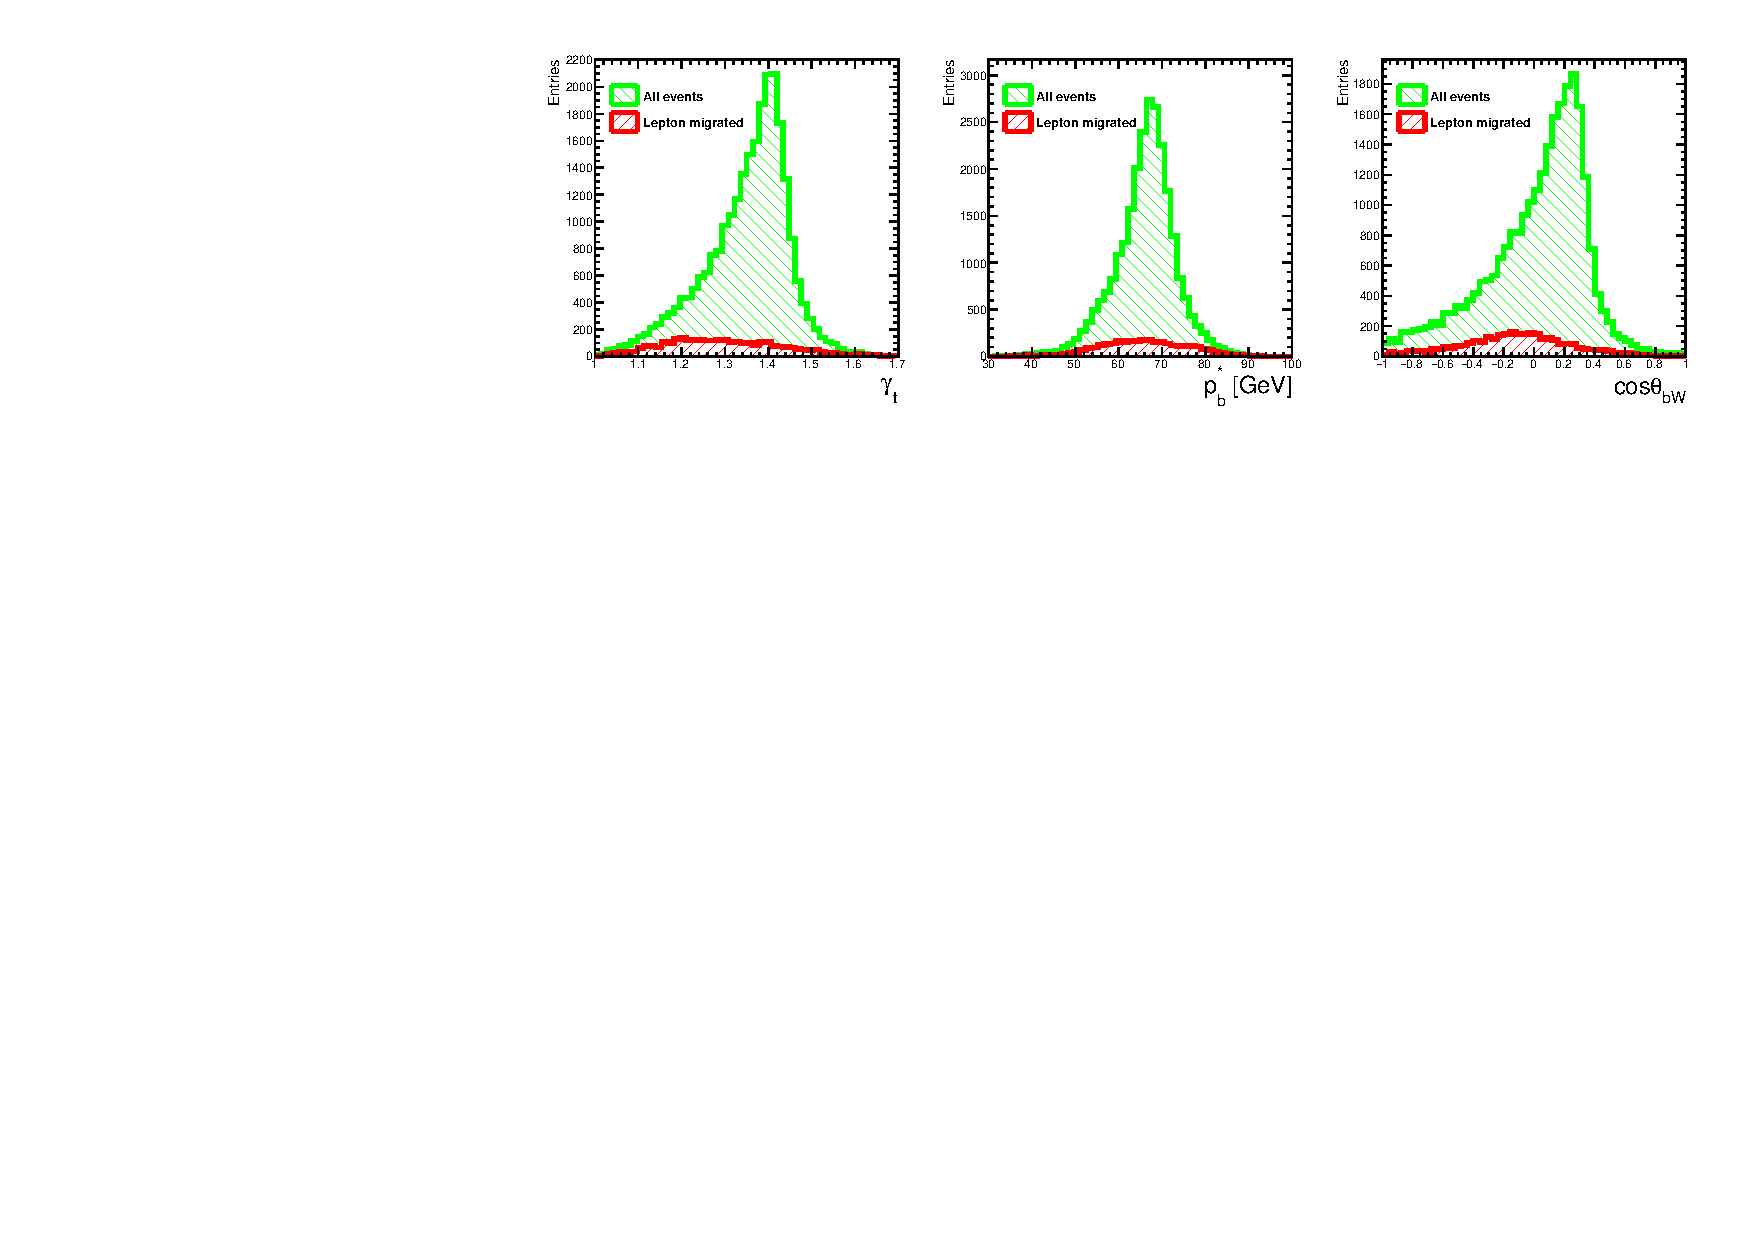
\includegraphics[clip, trim=0.1cm 0cm 13.75cm 0cm,width=0.99\textwidth]{ILD/plots/top-lepton-variables.pdf}
		\caption{\label{fig:TopChiVariables_a_3} }
	\end{subfigure}% 
	\begin{subfigure}{0.33\textwidth}
		\centering
		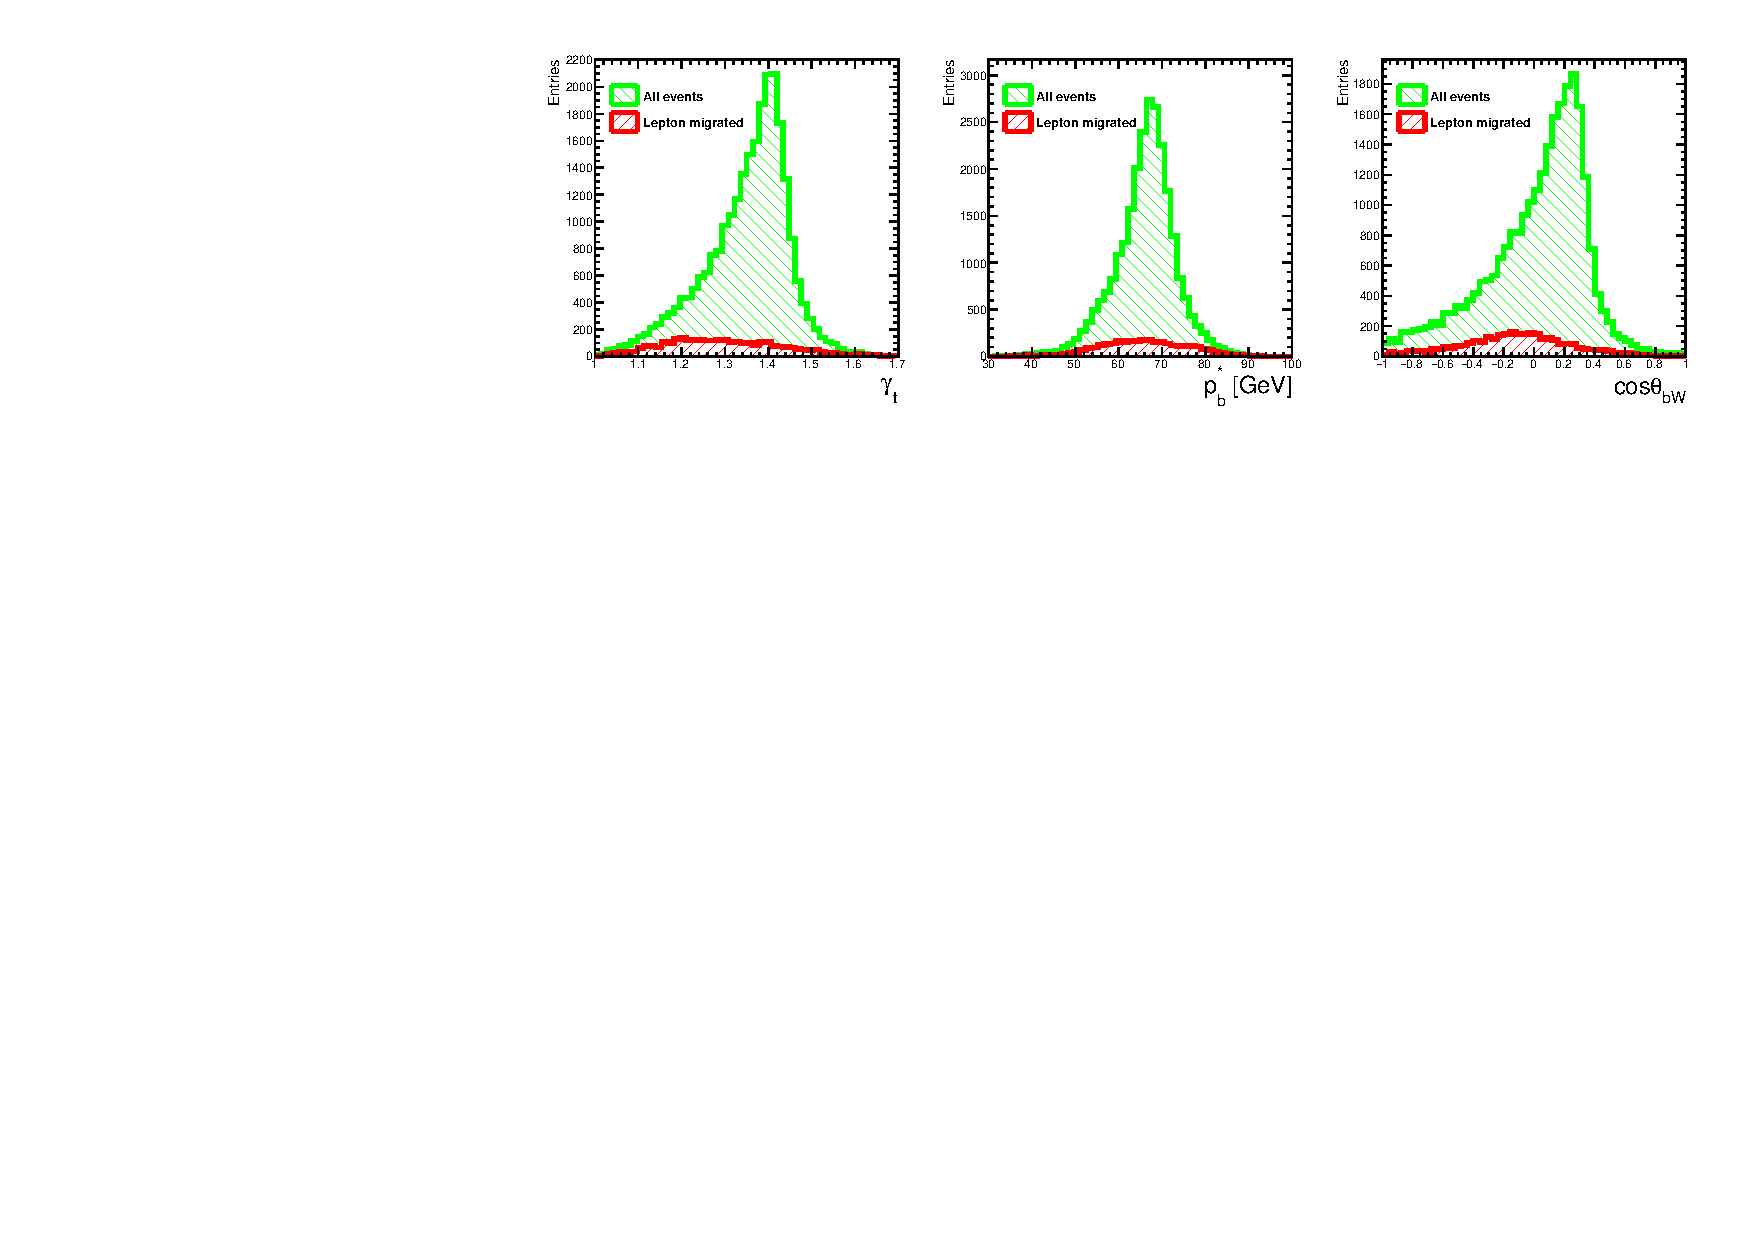
\includegraphics[clip, trim=6.78cm 0cm 7.1cm 0cm,width=0.99\textwidth]{ILD/plots/top-lepton-variables.pdf}
		\caption{\label{fig:TopChiVariables_b_3} }
	\end{subfigure}
	\begin{subfigure}{0.33\textwidth}
		\centering
		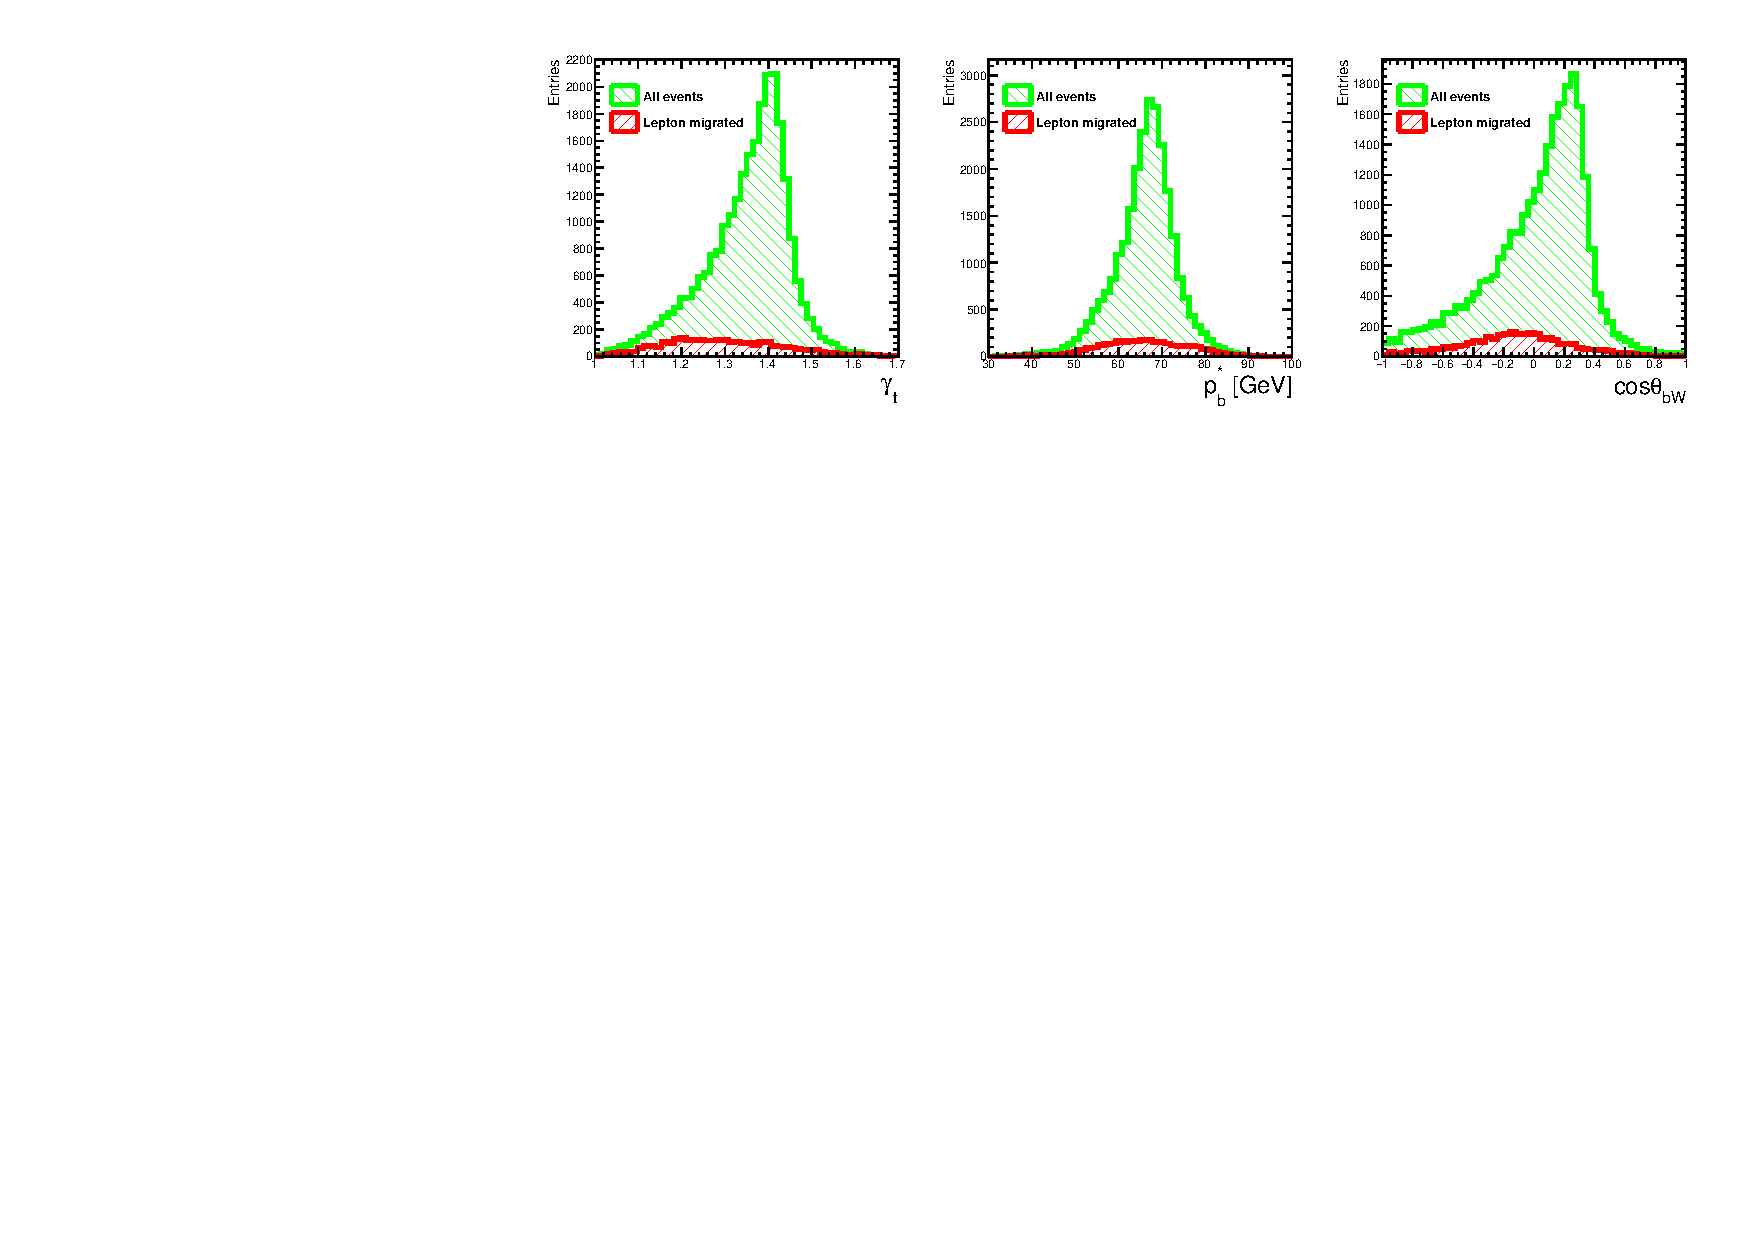
\includegraphics[clip, trim=13.6cm 0cm 0.4cm 0.cm,width=0.99\textwidth]{ILD/plots/top-lepton-variables.pdf}
		\caption{\label{fig:TopChiVariables_c_3} }
	\end{subfigure}
	\caption{\sl Distributions of $\gamma_t$ (a), $p^*_b$ (b) and $\cos\theta_{bW}$ (c) variables used for $W^\pm$ lepton charge reconstruction. The events are subdivided into correctly and incorrectly assigned lepton categories. }
	
	\label{fig:TopChiVariables_3}
\end{figure}


More than 93\% of the events with $\chi^2_{top} < 15$ have a correct combination of a b-jet with hadronic $W^\pm$, which propagates into a correct interpretation of the $W^\pm$ lepton charge.

The application of all possible pair combinations of the vertex charge, kaon charge and $W^\pm$ lepton charge to the top polar angle reconstruction shown in Fig.~\ref{fig:TopAsymmetryChi_a_3}. 


\begin{figure}
	\centering
	\begin{subfigure}{0.5\textwidth}
		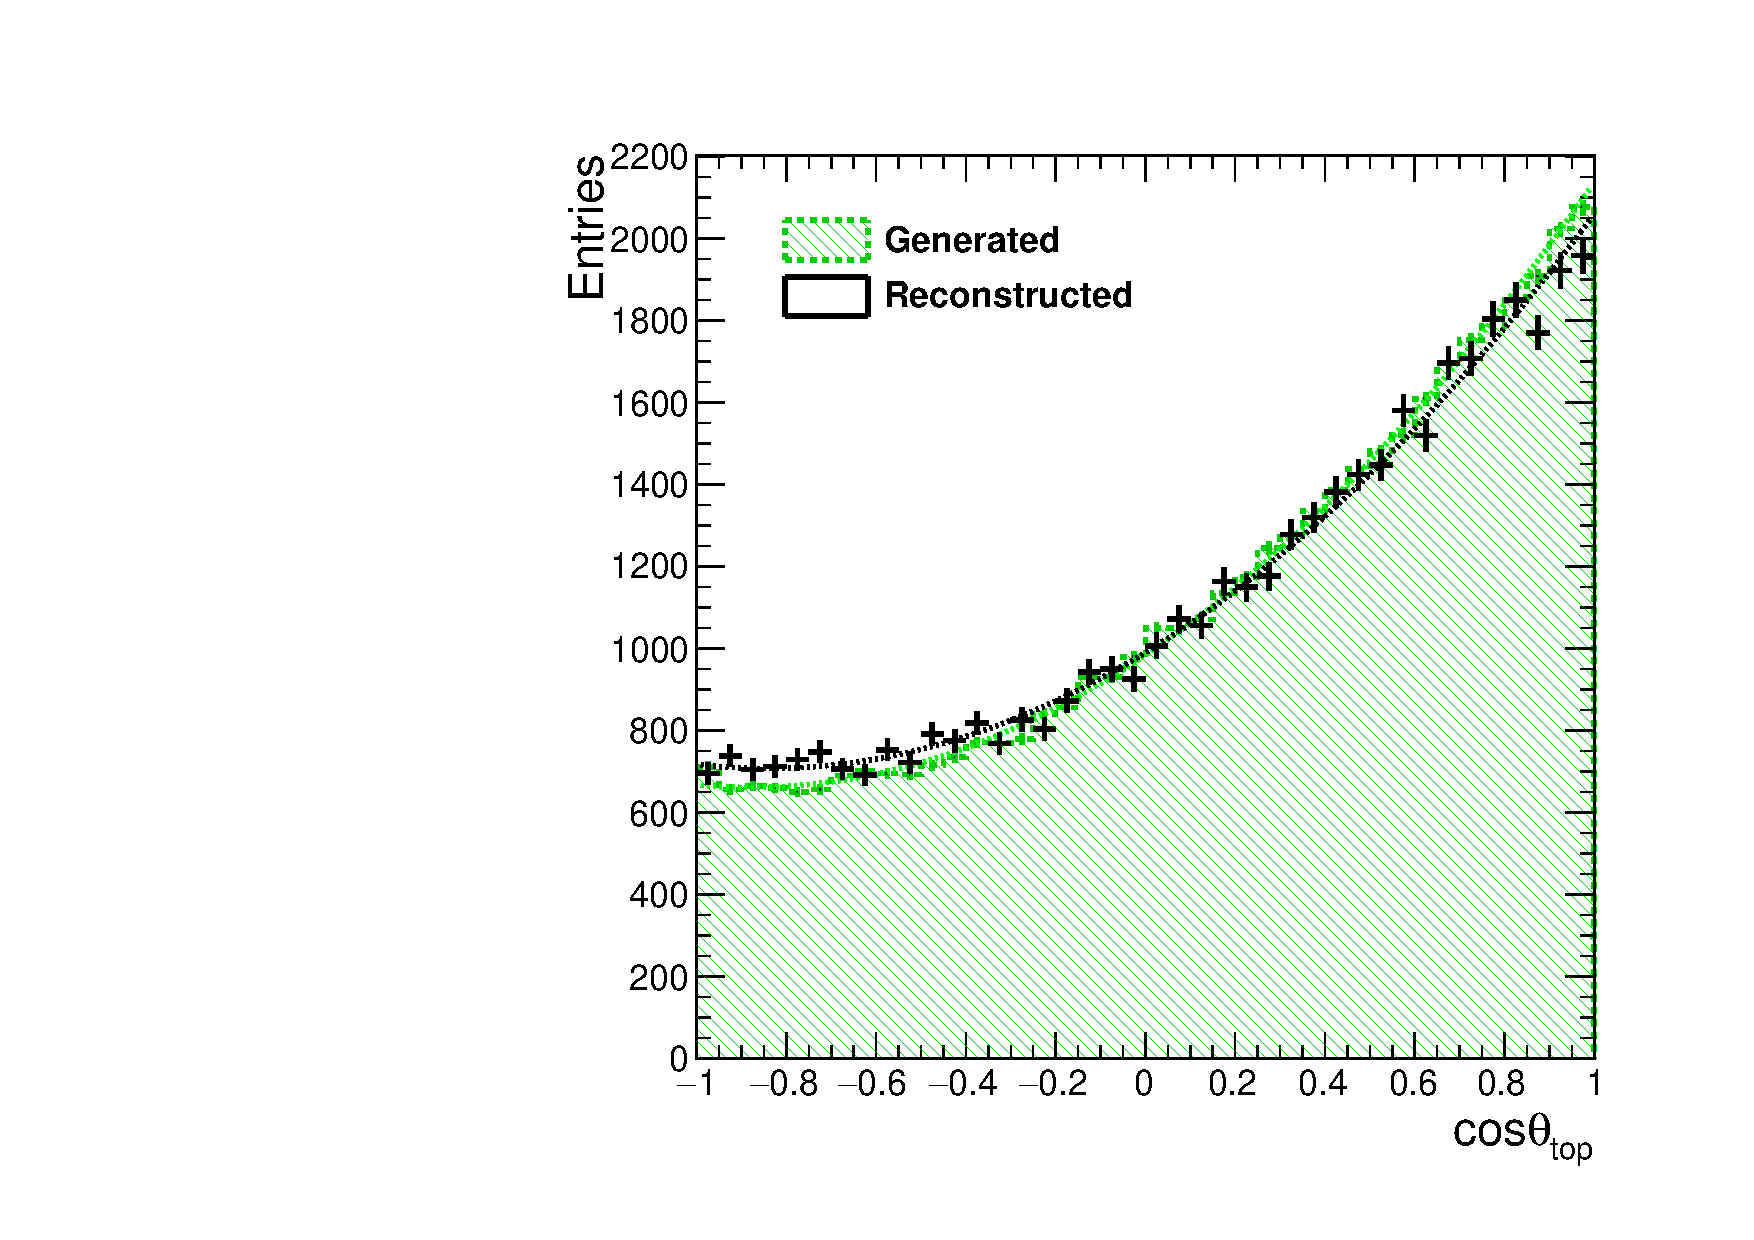
\includegraphics[width=0.95\textwidth]{ILD/plots/top-asymmetry-lepton.pdf}
		\caption{\label{fig:TopAsymmetryChi_a_3} }
	\end{subfigure}% 
	\begin{subfigure}{0.5\textwidth}
		\centering
		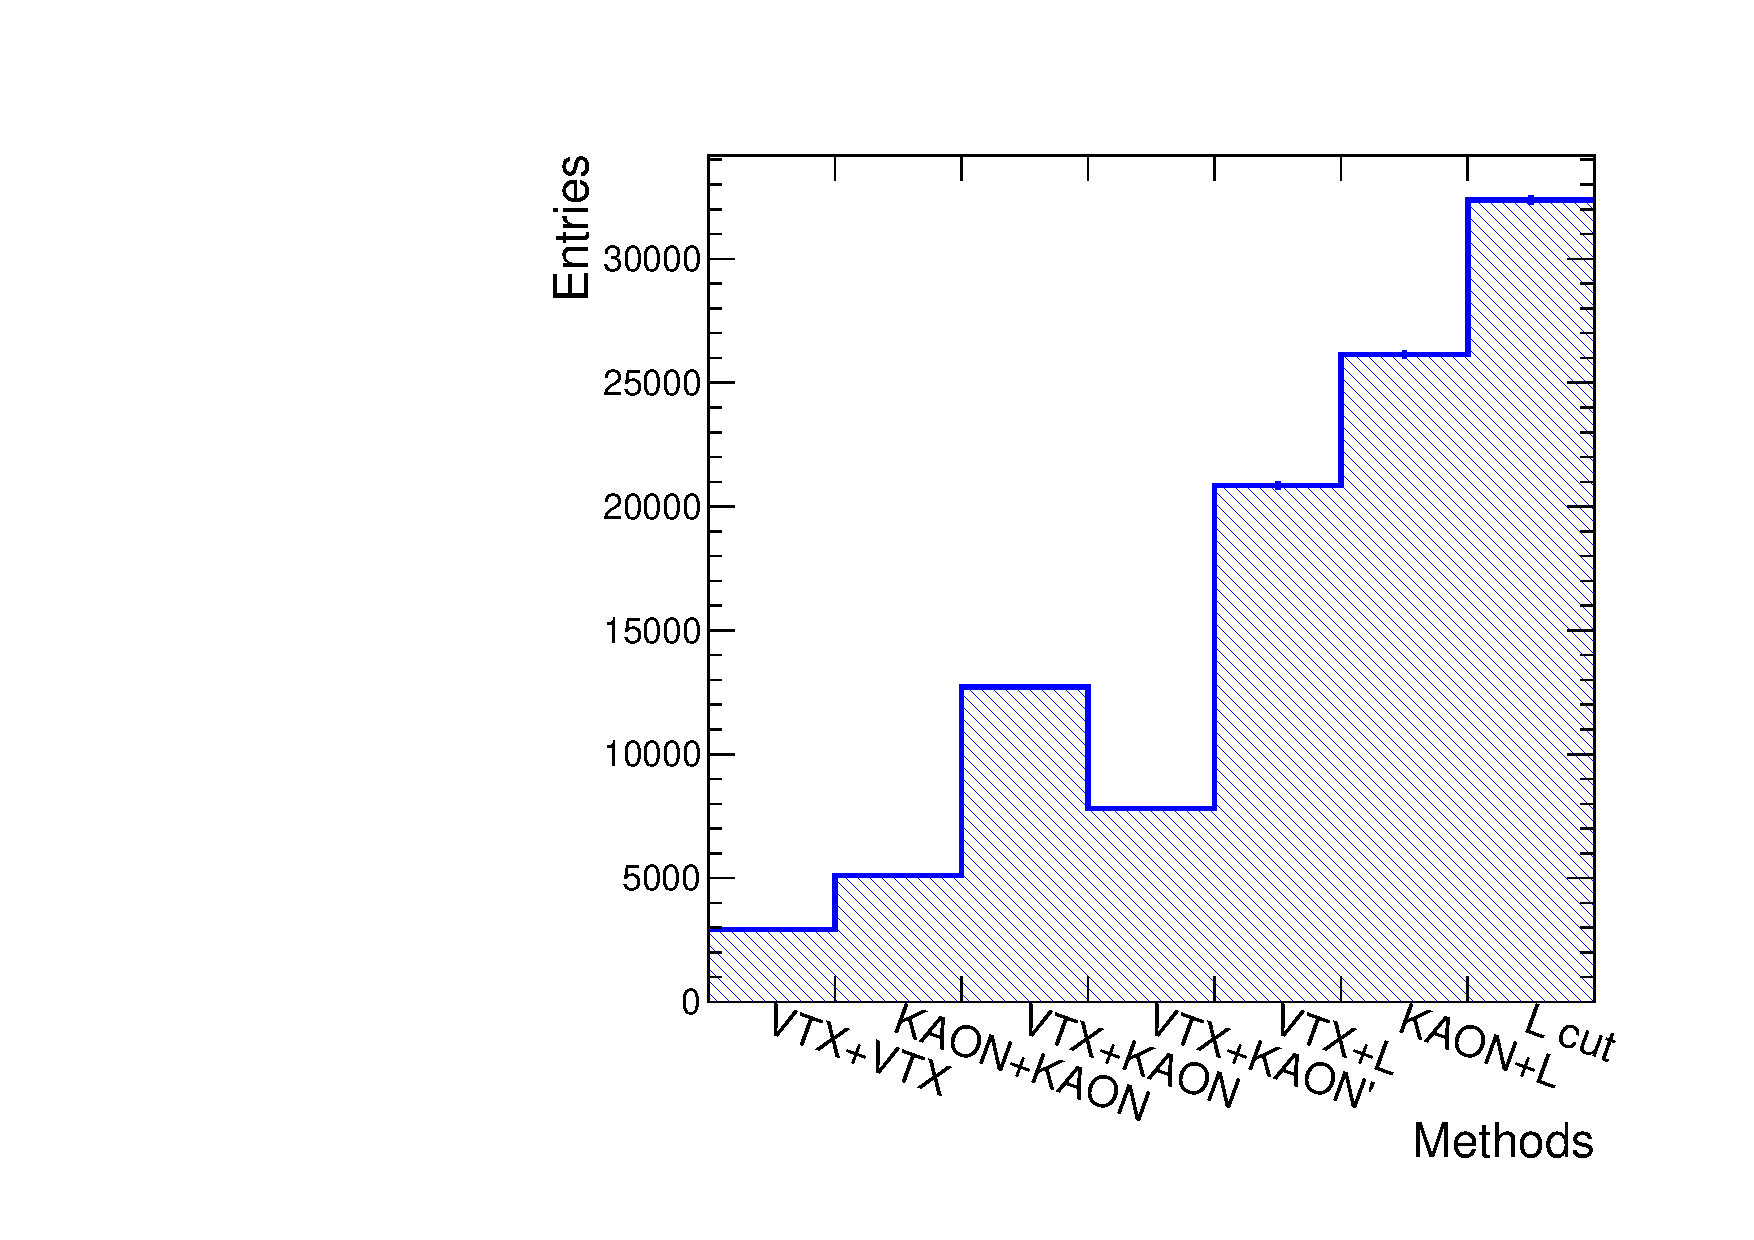
\includegraphics[width=0.95\textwidth]{ILD/plots/top-methods-lepton.pdf}
		\caption{\label{fig:TopAsymmetryChi_b_3} }
	\end{subfigure}
	\caption{\sl Generated polar angle distribution compared to reconstructed polar angle (a) using all possible charge signature combinations, plotted in (b). }
	\label{fig:TopAsymmetryChi_3}
\end{figure}

This method allows to reconstruct the top forward-backward asymmetry with $A_{FB}^{rec}/A^{gen}_{FB} = 94\%$ with the final efficiency of 38.6\%, which improves the previous result~\cite{bib:ILCTOP} by 25\%. 

The most used method is combination of the vertex charge with the $W^\pm$ lepton charge because the $W^\pm$ lepton is required to be reconstructed in every selected event. 
%\subsubsection{Precision on top quark form factors }
%%%%%%%%%%%%%%%%%%%%%%%%%%%%%%%%%%%%%%%%%%%%%%%%%%%%%%%%%%%
%%%%%%%%%%%%%%%%%%%%%%%%%%%%%%%%%%%%%%%%%%%%%%%%%%%%%%%%%%%
%%%%%%%%%%%%%%%%%%%%%%%%%%%%%%%%%%%%%%%%%%%%%%%%%%%%%%%%%%%

\subsection{Summary and outlook}

In this chapter, three basic signatures of the top quark charge were used: the vertex charge, the kaon charge and the $W^\pm$ lepton charge. 
It was found, that one has an event migration effect if only one signature is used to determine the top quark charge. 
However, a combination of the charge signatures give a satisfactory results.
As a proof of concept, only the vertex and kaon charge combination has been applied, which gave a good correspondence between the generated and the reconstructed top polar angle distributions.
As it was shown, the combination of the b-quark charge and the $W^\pm$ charge signatures significantly increases the statistics used for the top polar angle computation.

Besides the b-quark charge application, the statistics in the left-handed case can be increased by the reconstruction of the hadronic tau lepton decays, which were not used in the present studies. 
Another way to reduce the charge migration effects is to involve the leptonic top quark decays in the top reconstruction, which can give a hint to a correct top decay products association.

The b-quark charge measurement is a completely independent reconstruction tool, which allows studying and controlling the systematics effects.

The b-quark charge measurement is indispensable in case of the fully hadronic \ttbar\ decays, where there is no other sources of information about the top quark charge. 
In left-handed electron beam case, one directly applies the b-quark charge measurement, as it was done to produce the top quark polar angle distribution shown in Fig.~\ref{fig:TopAsymmetryNoCutBjet_3}. 
However, in the right-handed electron beam, the incorrect $W^\pm$ jets and b-jet association will lead to a significant distortion in the top polar angle distribution. Therefore, one should look for $W^\pm$ c-quark charge, using kaon charge, to control the top quark reconstruction quality. 


%%%%%%%%%%%%%%%%%%%%%%%%%%%%%%%%%%%%%%%%%%%%%%%%%%%%%%%%%%%%%%%%%
%%%%%%%%%%%%%%%%%%%%%%%%%%%%%%%%%%%%%%%%%%%%%%%%%%%%%%%%%%%%%%%%%
%%%%%%%%%%%%%%%%%%%%%%%%%%%%%%%%%%%%%%%%%%%%%%%%%%%%%%%%%%%%%%%%%
\newpage
\section{Bottom quark production at the ILC}
\label{sec:BProduction}
%Motivation
The LEP measurement of the forward-backward asymmetry at the $Z^0$ pole resulted in 2.5$\sigma$ deviation from the \sm\ prediction, which can be an impact of a \bsm\ modification of the b-quark couplings to vector bosons.
The resolution of the LEP \afbb\ deviation requires a new level of the experimental precision.
This is the main motivation of the $e^+e^-\to b\bar{b}$ studies at the $250$\,GeV stage of the ILC, which are presented in this chapter. 

The $e^+e^-\to b\bar{b}$ process has never been studied using the ILC environment. 
\subsection{Setup of the study}
In this studies the signal process is $e^+e^-\to b\bar{b}$ on the center-of-mass energy of 250\,GeV. 
A large statistics sample of integrated luminosity $L_{int}= 250$\,fb{$^{-1}$} is used for both polarizations in the ILD simulation environment. 
Same version of the event generators and the {\sc ilcsoft} distribution as for the \ttbar\ study are used.
The kaons from the secondary or tertiary vertices are reconstructed using the generator information, but with impurity and inefficiency of the direct kaon reconstruction, described in Sec.~\ref{sec:Kaons}.


\subsection{Bottom quark reconstruction and the background rejection}
The bottom quarks hadronize into two b-jets in the detector, that are reconstructed by jet clustering algorithm. %, which significantly simplifies the process reconstruction. 

%The \bbbar\ events are simply reconstructed as a simple two jet event, which are sorted by the b-tag value.
An example of the \bbbar\ pair event display in the ILD environment is shown in Fig.~\ref{fig:BottomEvent_3}. As one sees from the Table~\ref{table:bbbarselection}, the largest background is the \bbbar\ $Z^0$ return events, which is also true for the right-handed beam configuration, due to large $e^+e^-\to Z^0\gamma$ process cross section.
\begin{figure}
	{\centering
		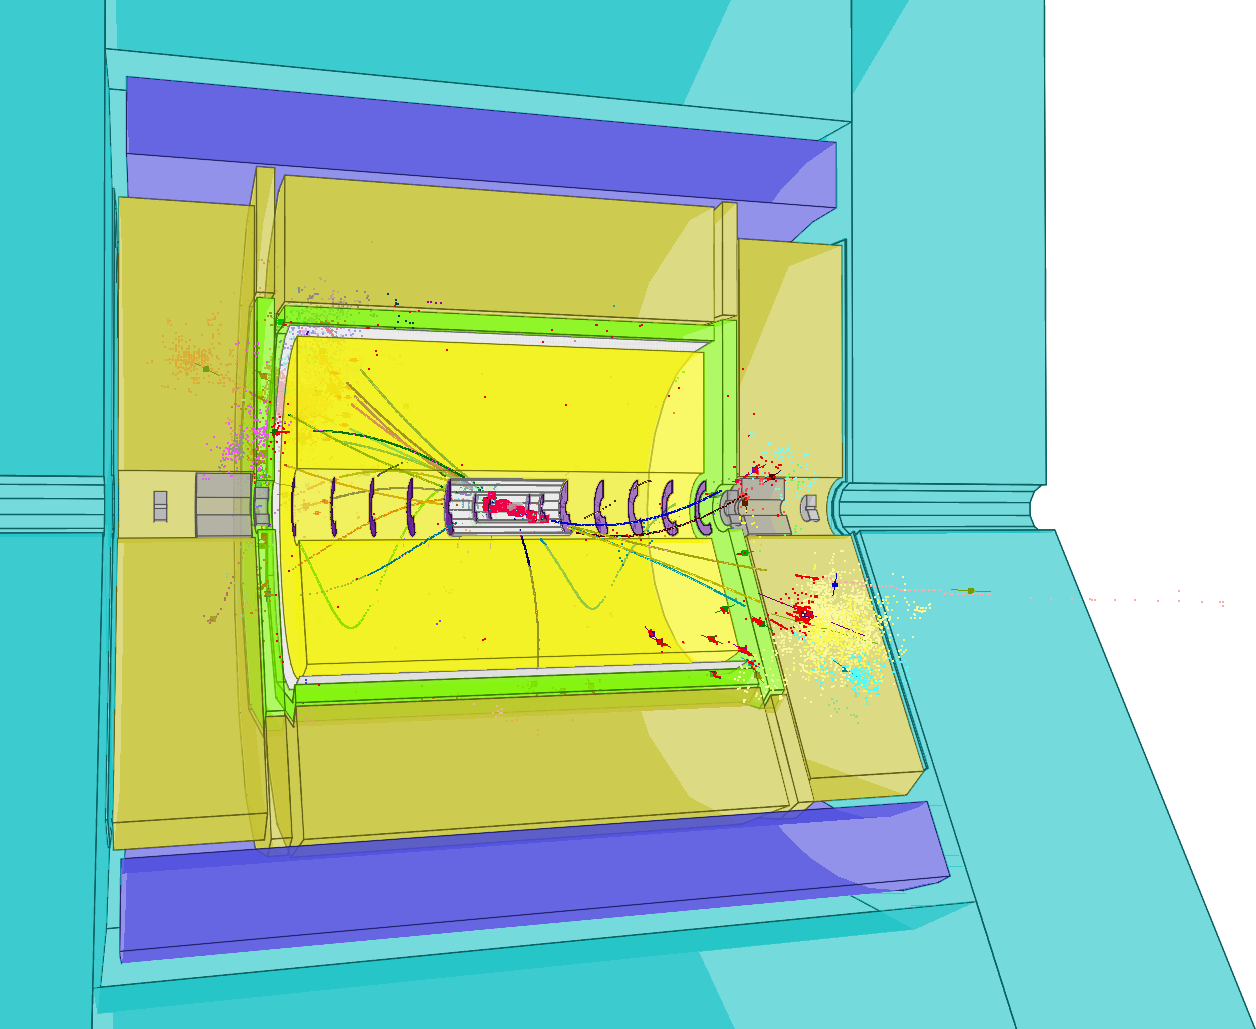
\includegraphics[clip, trim=0.cm 0cm 7.9cm 0cm, width=0.55\textwidth]{ILD/graphics/ild-bbbar.png}
		\caption{\sl Event display of the $e^+e^-\to b\bar{b}$ process in the ILD simulation.
		}
		\label{fig:BottomEvent_3}
	}
	
\end{figure}
% Signal has high cross section -> but, background can distort polar angle spectrum, -> background levels >  cuts -> results 

%The main challenge is to reject the background processes, which can distort the reconstructed polar angle spectrum of the b-quark. 
The most significant background processes are the so called $Z^0$ return background and the hadronic decays of diboson processes, like the hadronic decays of $e^+e^-\to Z^0Z^0$ or $e^+e^-\to Z^0H$ process. The process $e^+e^-\to W^\pm W^\mp$ has higher cross section than the signal, but the $W^\pm$ bosons have small branching ratio to the b-quark, hence, this process is easily rejected by b-tag cuts. 
The analysis benefits from the large production cross section, as compared to the background processes, as shown in Table~\ref{table:bbbarsigma}.

The $Z^0Z^0$ and $Z^0H$ pairs have large branching fractions to the b-quarks. 
As one sees from the Table~\ref{table:bbbarselection}, the largest background contribution is coming from the \bbbar\ $Z^0$ return events, which is also true for the right-handed beam configuration, due to the large $e^+e^-\to Z^0\gamma$ process cross section.

The defined cuts against the background processes are the following:
\begin{itemize}
	\item Value of the first jet b-tag should be higher than 0.8 and b-tag of the second jets is higher 0.3;
	\item Invariant mass of two jets $m_{Inv} > 180$\,GeV and maximal photon energy $E^{max}_\gamma < 40$\,GeV;
	\item Sum of the jet masses $m^{jet}_1+m^{jet}_2<120$\,GeV;
%	\item Sphericity of the event, which is defined as $S_{I} = \sum p_i / E$, should be less than 0.2.
\end{itemize}
The sum of the jet masses is changing with the b-jet polar angle as shown in Fig.~\ref{fig:JetMasses_3}. This deviation happens due to the degrading jet energy resolution towards the forward region of the detector. 
\begin{figure}
	{\centering
		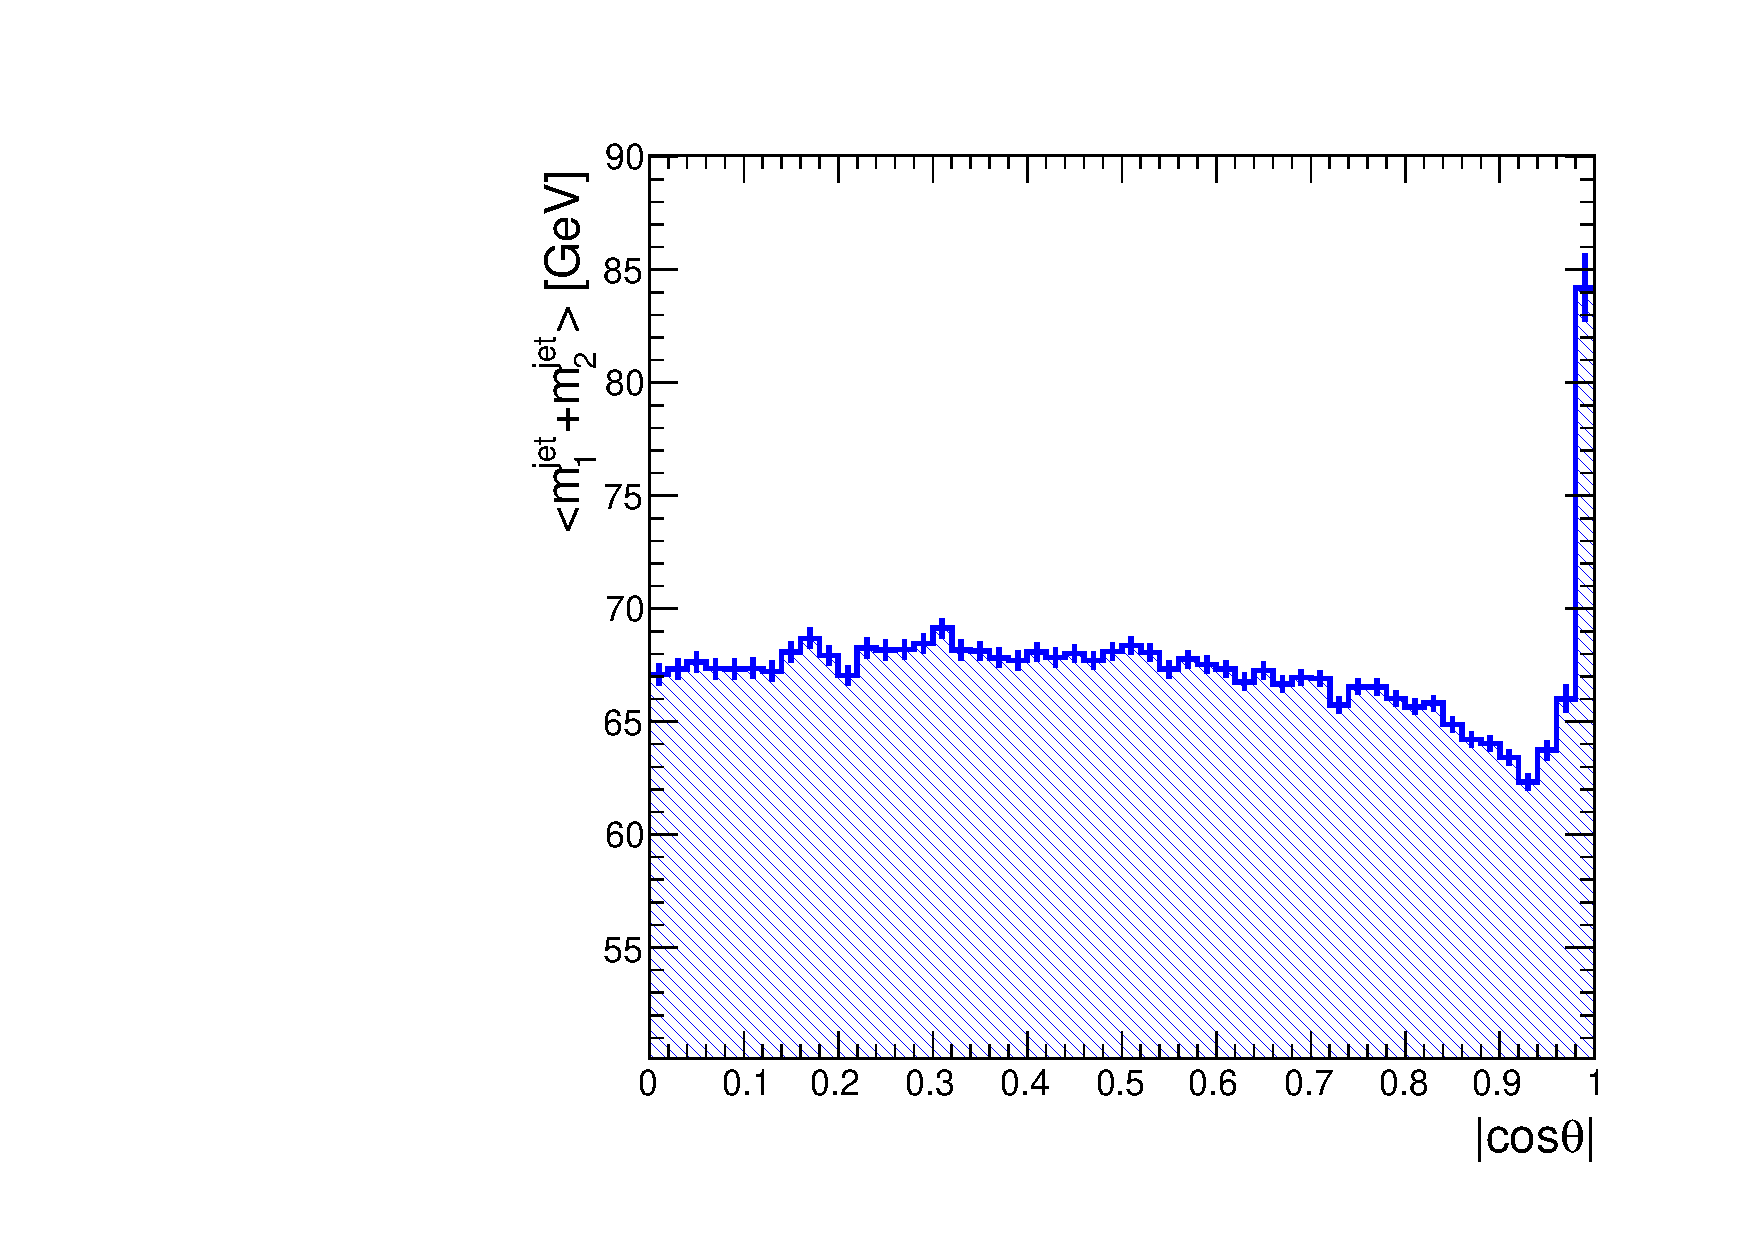
\includegraphics[width=0.55\textwidth]{ILD/plots/mass-correction.pdf}
		\caption{\sl Mean sum of the jet masses as function of the polar angle of b-jets.   
		}
		\label{fig:JetMasses_3}
	}
	
\end{figure}
This behavior cause a bias in the b-quark polar angle distribution after the cut on  $m^{jet}_1+m^{jet}_2$ value. 
Thus, a polar angle correction was introduced to remove the $m^{jet}_1+m^{jet}_2$ dependence on the $|\cos\theta|$.
These cuts and the angular correction are applied equally to both beam polarizations.
The successive application of the preselection cuts is demonstrated in Table~\ref{table:bbbarselection}.

        \begin{table}[H]
        \begin{center}
        \begin{tabular}{l c c c}
        \hline
	Channel & $\sigma_{unpol.}$\ [fb] & $\sigma_{LR}$ [fb] &  $\sigma_{LR}$ [fb] \\
	\hline
	$b\bar{b}$ & 1756 & 5629 & 1394 \\
	\hline
%	$c\bar{c}$ & 2884 & 8033 & 3502 \\
	$\gamma b\bar{b}$ ($Z^0$ return) & 7860 & 18928 & 12512 \\
%	$W^\pm W^\mp $ &3152&12383&225 \\ 
	$Z^0Z^0$ hadronic &501 & 1402 & 604 \\
	$Z^0Z^0$ semileptonic  &534 & 1425 & 709\\
	$HZ^0$ hadronic  &143 & 351 & 222 \\
        \hline
        \end{tabular}
        \end{center}
        \caption{\sl Unpolarized and 100\% polarized cross sections at the Born level forthe  signal and the background processes at $\sqrt{s}=250$\,GeV. The cross section values are estimated using Whizard generator.}
        \label{table:bbbarsigma}
        \end{table}


%This signal selection technique  aimed at a very high purity, for the left-handed beam configuration the selection purity is 98.2\% and for the right-handed beam the final efficiency is the same 48\%, but the purity is decreased - 95\%, because of smaller signal cross section.

        \begin{table}[H]
        \begin{center}
        \begin{tabular}{l c c c c}
        \hline
	Selection criteria & \bbbar & $Z^0Z^0$ hadronic  & $HZ$ hadronic &  $Z^0$ return   \\
	\hline
	Initial & 1698477 & 350647 & 345134 & 258843 \\
	b-tag cuts & 1104853 (65.05\%) & 57300 (16.34\%) & 134324 (38.92\%) & 105638 (40.81\%) \\
	$m_{Inv}$ and $E_\gamma^{max}$ cut & 932512 (54.90\%) & 53172 (15.16\%) & 127003 (36.80\%) &  505 (0.20\%) \\
	$m_1+m_2$ cut & 877012 (51.64\%) & 9239 (2.63\%) & 16517 (4.79\%) & 473 (0.18\%) \\
	Sphericity cut & 827651 (48.73\%) & 5512 (1.57\%) & 7812 (2.26\%) & 422 (0.16\%) \\
        \hline
        \end{tabular}
        \end{center}
        \caption{\sl Efficiency of signal and non-\ttbar\ backgrounds after different cuts for left-handed beam polarization~[Jeremy]}
        \label{table:ttbarselection}
        \end{table}



\subsection{Results}
\label{sec:BBBarresults}
In these studies the same approach as for \ttbar\ polar angle computation is applied. In \bbbar\ process analysis, one has no other charge information sources available, except the b-jet information. 
Therefore, in this chapter, only the reconstructed vertex charge and kaon charge are computed and applied to the b-quark polar angle reconstruction. 

\subsubsection{Polar angle reconstruction}
In this section, the reconstruction of the signal process only is discussed using standard ILD reconstruction. %without application of vertex charge recovery algorithm.

The b-quark polar angle is defined as a polar angle of the vector
\begin{equation}
	\vec{p}_{b\bar{b}} = \vec{p}_{b} - \vec{p}_{\bar{b}},
\end{equation}
where $\vec{p}_{b}$ and $\vec{p}_{\bar{b}}$ are the momentum vector of the reconstructed b-quark jet and anti b-quark jet, respectively.
%computed as the vector difference polar angle of two b-jets after charge calculation. 
Figure~\ref{fig:BAsymmetryFirst_3} demonstrates reconstructed b-quark polar angle compared to the generated distribution for both beam polarizations. 
The generated $A_{FB}^{gen}$ values are:
\begin{equation}
	A_{FB}^{gen}(e^-_L e^+_R) = 0.705\text{ and }A_{FB}^{gen}(e^-_R e^+_L) = 0.26.
\end{equation} 
The difference in the generated b-quark polar angle distributions for two polarization configurations are caused by the different the $Z^0$ boson couplings to the left-handed and the right-handed fermions. 

\begin{figure}
	\centering
	\begin{subfigure}{0.5\textwidth}
		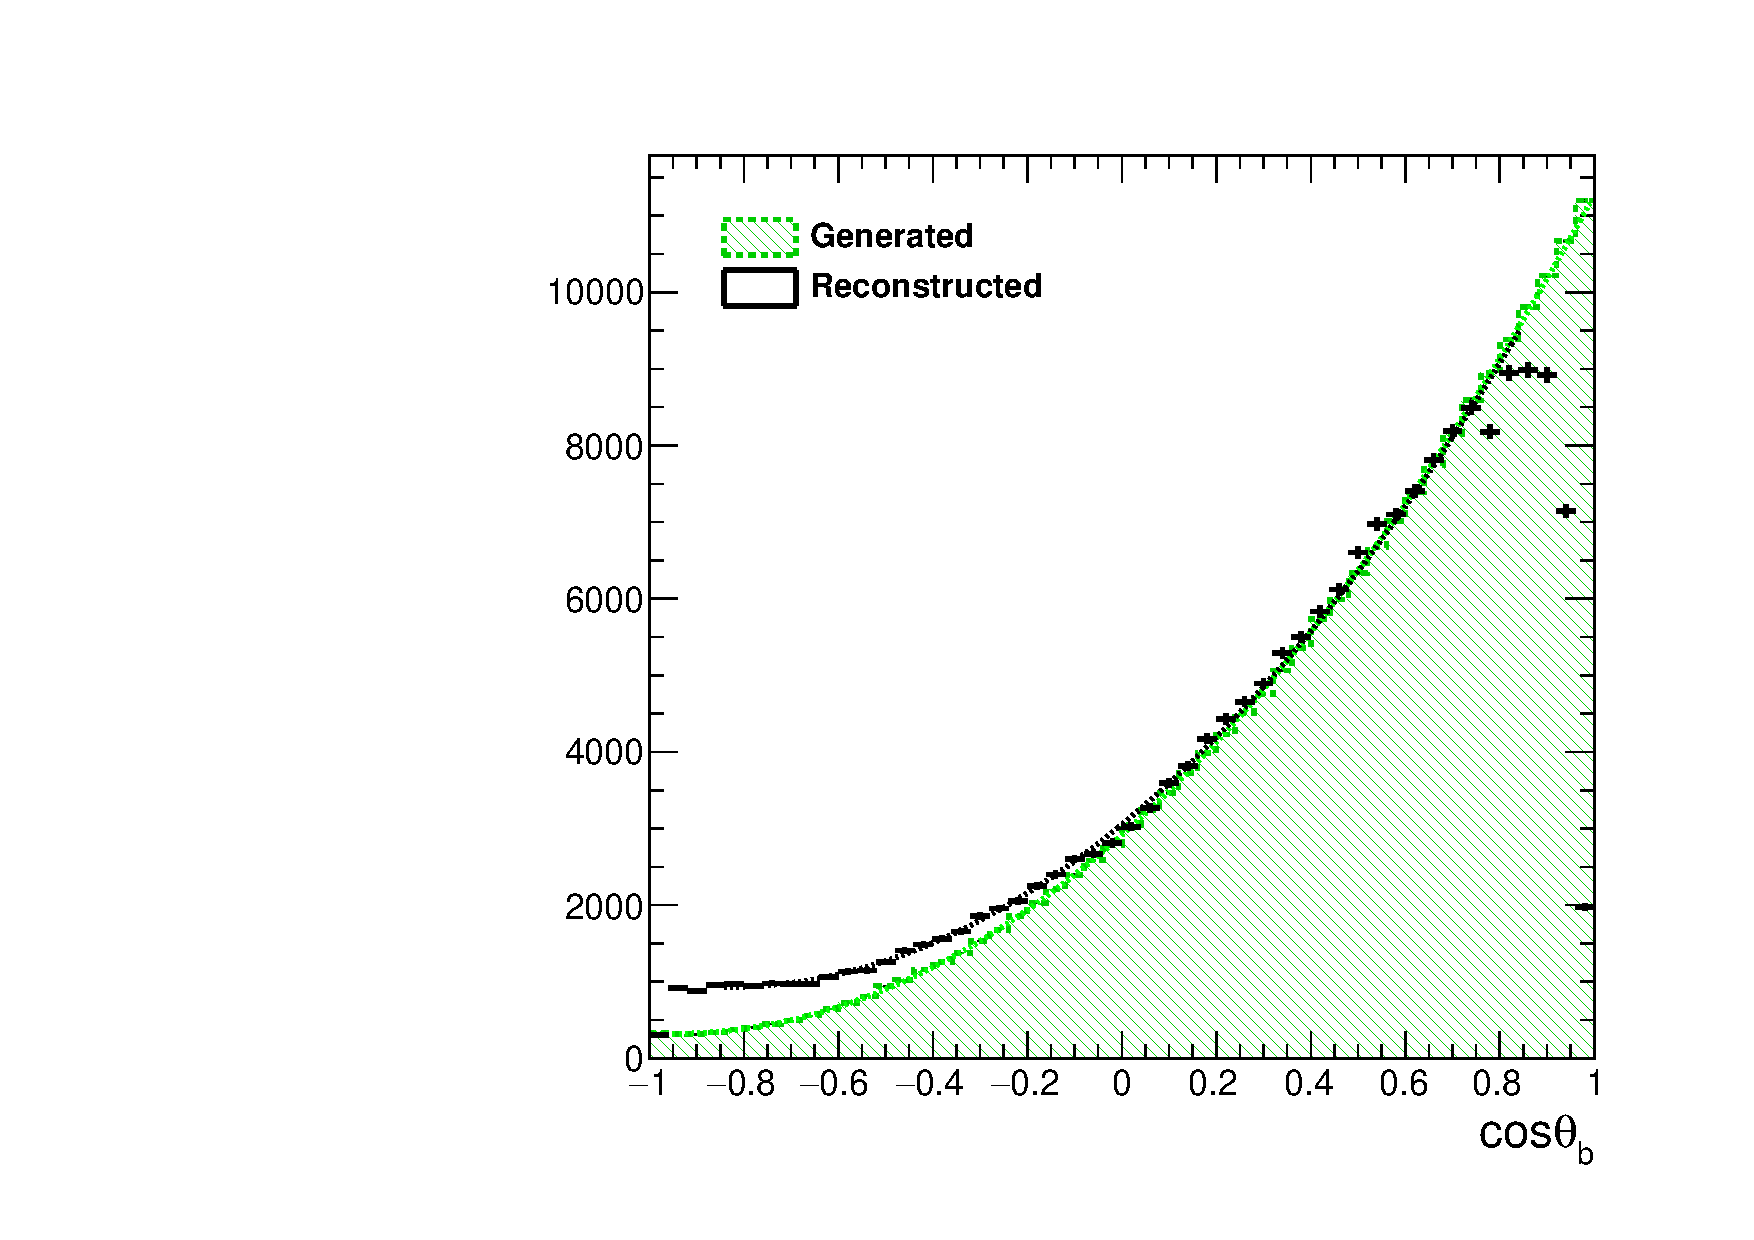
\includegraphics[width=0.95\textwidth]{ILD/plots/basymmetry-norec-nocorr-nobkg-left.pdf}
		\caption{\label{fig:BAsymmetryFirst_a_3} }
	\end{subfigure}% 
	\begin{subfigure}{0.5\textwidth}
		\centering
			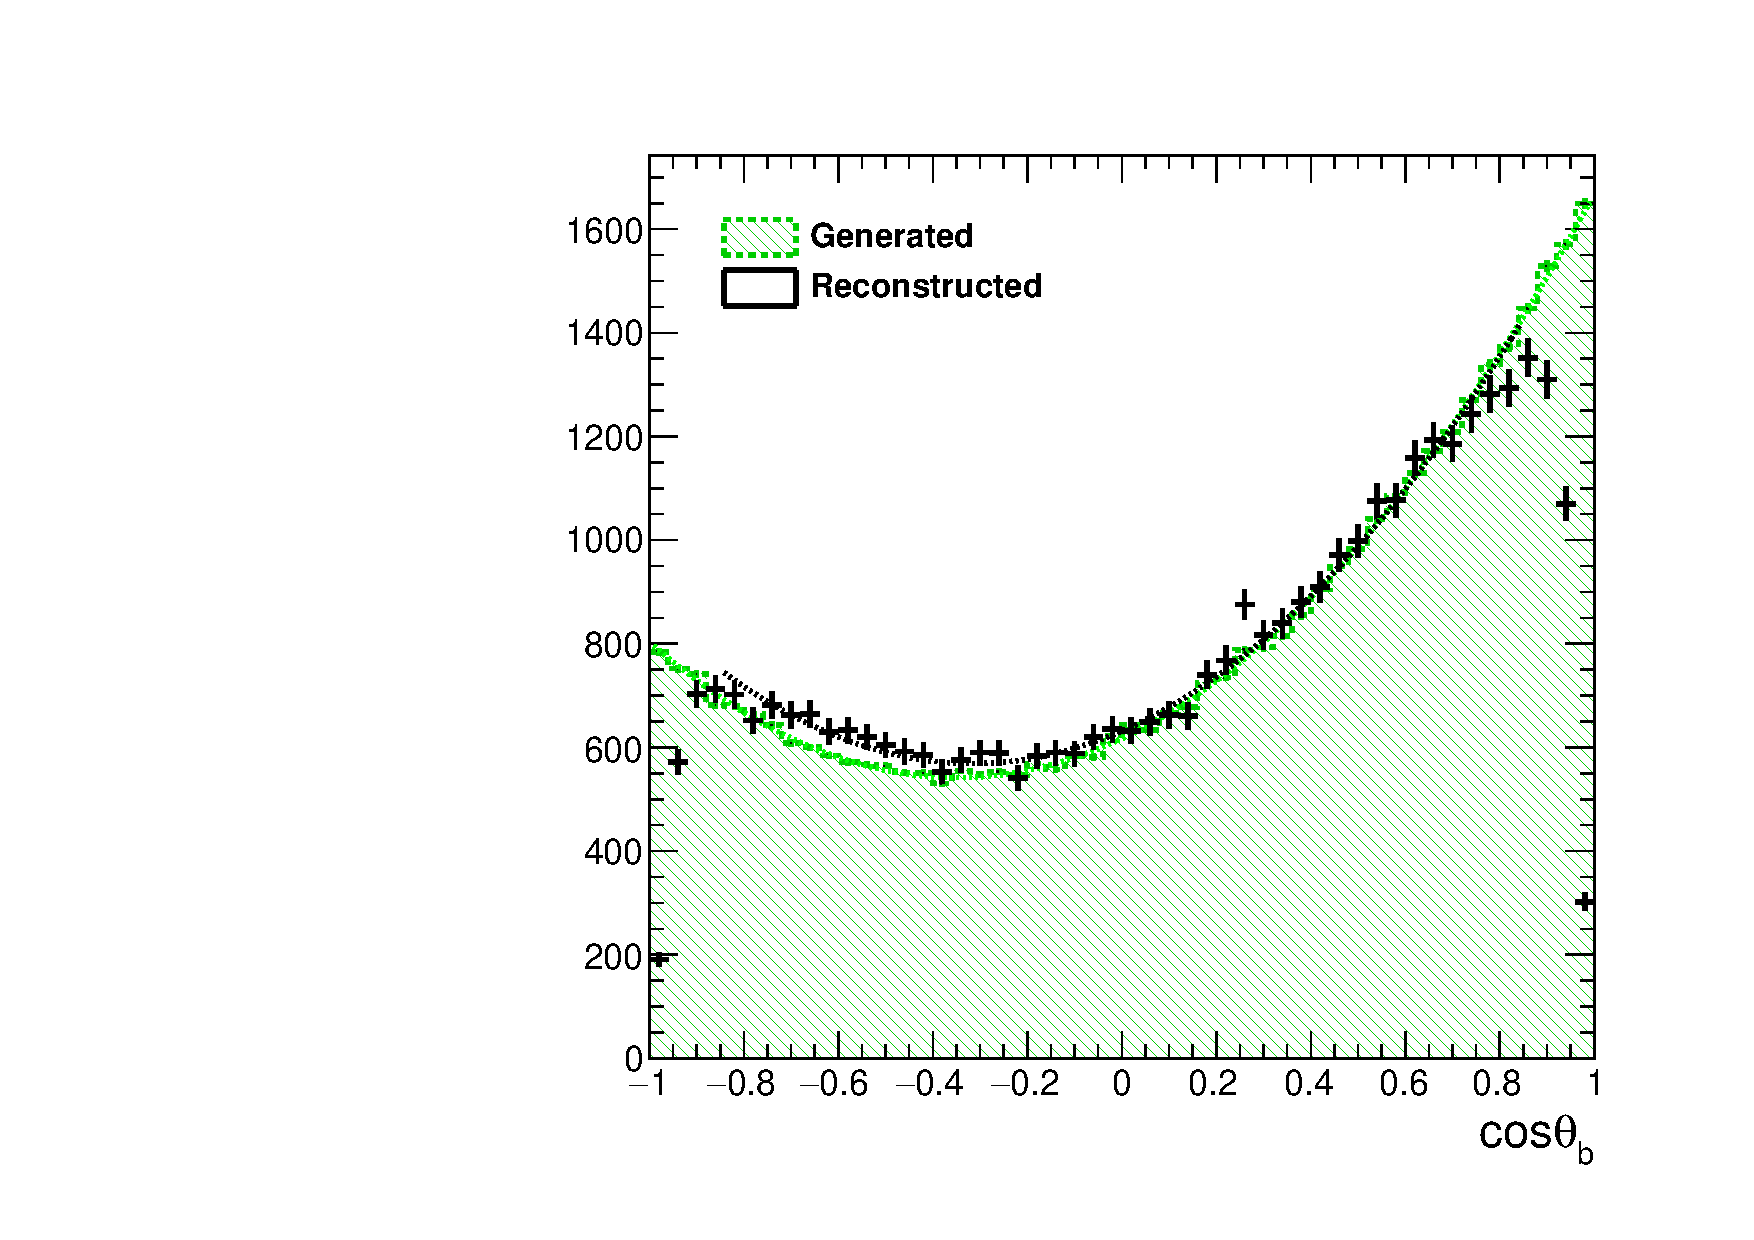
\includegraphics[width=0.95\textwidth]{ILD/plots/basymmetry-norec-nocorr-nobkg-right.pdf}
		\caption{\label{fig:BAsymmetryFirst_b_3} }
	\end{subfigure}
	\caption{\sl Generated b-quark polar angle distribution compared to reconstructed polar angle in left-handed case (a) and right-handed case (b) using all possible charge signature combinations. Integrated luminosity used 250\ifb for both polarizations. }
	\label{fig:BAsymmetryFirst_3}
\end{figure}
%Both polarizations
The reconstructed b-quark polar angle distributions have two major problems:
\begin{itemize}
	\item The residual charge impurity flips the polar angle from $\cos\theta$ to $-\cos\theta$ and it contaminates the backward region $\cos\theta < 0$ of both distributions in Fig.~\ref{fig:BAsymmetryFirst_3}. Due to the strong b-quark production asymmetry in the left-handed case the backward region is fully contaminated by the events with misreconstructed b-quark charge as seen in Fig.~\ref{fig:BAsymmetryProblem_a_3}.
	\item The large efficiency decrease in the forward region $|\cos\theta| > 0.85$. The main reason of this decrease is the inefficiency of the vertexing algorithms, which tend to not find any reconstructed vertex in the forward region, as seen in Fig.~\ref{fig:MissedCos_3}. The zoom into the problematic region is shown in Fig.~\ref{fig:BAsymmetryProblem_b_3};

\end{itemize}


\begin{figure}
	\centering
	\begin{subfigure}{0.5\textwidth}
		\includegraphics[width=0.95\textwidth]{ILD/plots/basymmetry-zoom-contamination.pdf}
		\caption{\label{fig:BAsymmetryProblem_a_3} }
	\end{subfigure}% 
	\begin{subfigure}{0.5\textwidth}
		\centering
		\includegraphics[width=0.95\textwidth]{ILD/plots/basymmetry-zoom-inefficiency.pdf}
		\caption{\label{fig:BAsymmetryProblem_b_3} }
	\end{subfigure}
	\caption{\sl The demonstration of the contamination of backward region by the events with misreconstructed charge (a) and the forward region inefficiency of the b-quark polar angle measurements (b). }
	\label{fig:BAsymmetryProblem_3}
\end{figure}

The  inefficiency in the forward region of the detector makes impossible the measurement of the $A_{FB}^b$ using a simple counting method. 
%This problem can be avoided by the fitting the unaffected central bins with a function and extrapolating the fitted function on the full polar angle range $(-1,1)$. 
Thus, the b-quark polar angle analysis limited to the region of $|\cos\theta| < 0.8$.
The polar angle histogram is fitted by a general differential cross section function as:
\begin{equation}
	f(A,B) = S(1+\cos^2\theta) + A \cos\theta, %+ C \sin^2\theta,
	\label{formula:PolarAngleFit_3}
\end{equation}
where $S$ and $A$ are the fitted parameters. 
The parameter $S$ is proportional to the total cross section, while $A$ is proportional to the forward-backward asymmetry.
After the fit, the function is extrapolated to the full polar angle spectrum.
However, the sensitivity of the current ILD experiment configuration to New Physics effects is lost for $|\cos\theta| > 0.85$.

In this chapter, the forward-backward asymmetry is used as a measure of the polar angle reconstruction quality.
Using the extracted polar angle function the reconstructed $A_{FB}^b$ value is calculated as
\begin{eqnarray}
	A_{FB} = \frac{3}{8}\frac{A}{S}.
\end{eqnarray} 
The precision of the $A_{FB}^b$ reconstruction is $A_{FB}^{rec}/A^{gen}_{FB} = 88\%$ in left-handed case and  $A_{FB}^{rec}/A^{gen}_{FB} = 89\%$ in the right-handed case.  
However, the backward region contamination problem requires large corrections for residual charge misreconstruction in the left-handed polarization case as compared to the right-handed polarization case. 

%The method of b-quark polar angle correction should be independent from the generated curve. 

\subsubsection{Vertex Charge Recovery influence}

In this section, the vertex charge recovery algorithm, described in Section~\ref{sec:VtxRecovery}, is applied to the b-quark polar angle measurement in attempt to decrease the discrepancies between generated and reconstructed distributions.
The result of the recovery application is shown in Fig.~\ref{fig:BAsymmetryRec_3}.
\begin{figure}
	\centering
	\begin{subfigure}{0.5\textwidth}
		\includegraphics[width=0.95\textwidth]{ILD/plots/basymmetry-rec-nocorr-nobkg-left.pdf}
		\caption{\label{fig:BAsymmetryRec_a_3} }
	\end{subfigure}% 
	\begin{subfigure}{0.5\textwidth}
		\centering
		\includegraphics[width=0.95\textwidth]{ILD/plots/basymmetry-rec-nocorr-nobkg-right.pdf}
		\caption{\label{fig:BAsymmetryRec_b_3} }
	\end{subfigure}
	\caption{\sl Generated b-quark polar angle distribution compared to reconstructed polar angle in left-handed case (a) and right-handed case (b) using the independent kaon and vertex charge combinations after application of the vertex charge recovery algorithm. }
	\label{fig:BAsymmetryRec_3}
\end{figure}
The main improvements of the vertex charge recovery are the following:
\begin{itemize}
	\item The number of accepted events is improved by 9\%;
	\item The $A_{FB}$ reconstruction is improved before correction by 3\%;
	\item The vertex charge purity is increased by 4\%;
	\item The kaon charge purity stays the same, but the number of kaons is increased by 10\%; 
	\item The vertex charge recovery provides close to constant charge purity in the barrel region of the ILD experiment, as can be seen in Fig.~\ref{fig:BAsymmetryRecZ_3}. This is the consequence of the recovery of the peaks of missing vertex particles as it is described in Sec.~\ref{sec:VtxRecovery}.
	The residual efficiency decrease in the $|\cos\theta|\approx 0.8$ bin is caused by the jet energy resolution.  
\end{itemize}

\begin{figure}
	\centering
	\begin{subfigure}{0.5\textwidth}
		\includegraphics[width=0.95\textwidth]{ILD/plots/zoom-rec.pdf}
		\caption{\label{fig:BAsymmetryRecZ_a_3} }
	\end{subfigure}% 
	\begin{subfigure}{0.5\textwidth}
		\centering
		\includegraphics[width=0.95\textwidth]{ILD/plots/zoom-norec.pdf}
		\caption{\label{fig:BAsymmetryRecZ_b_3} }
	\end{subfigure}
	\caption{\sl The demonstration of the vertex charge recovery improvement (a) compared to the standard algorithm (b). }
	\label{fig:BAsymmetryRecZ_3}
\end{figure}

%%%%%%%%%%%%%%%%%%%%%%%%%%%%%%%%%%%%%%%%%%%%%%%%%%%%%%
%%%%%%%%%%%%%%%%%%%%%%%%%%%%%%%%%%%%%%%%%%%%%%%%%%%%%%
%%%%%%%%%%%%%%%%%%%%%%%%%%%%%%%%%%%%%%%%%%%%%%%%%%%%%%
%Make sure no generated quantity used
\subsubsection{Charge purity measurement}
\label{sec:ChargePurity}
The knowledge of the charge purity from the reconstructed events, or the future ILC data is essential for the present analysis. 
%The adopted system of the
The measurement of the b-quark charge purity is done using the number of accepted events $N_a$ and the number of rejected events $N_r$. 
The b-quark charge measurement uses two compatible charge combinations, either the vertex charge or the kaon charge.
 Which means, that the following rules are applied:
\begin{itemize}
	\item To accept an event one need to measure both charges correctly, or both charges incorrectly;
	\item The rejected event has one charge correctly reconstructed and another incorrectly reconstructed. 
\end{itemize}

Let $p$ be a probability of a correct charge measurement, then $q = 1-p$ is a probability of the incorrect charge measurement. 
%Suppose, one has $N$ events, which is a sum of accepted event number $N_a$ and rejected event number $N_r$. 
Then, the number of accepted events is:
\begin{equation}
	N_a = N p^2 + N q^2,
	\label{formula:PurityA_3}
\end{equation}
while the number of rejected has the following expression:
\begin{equation}
	N_r = 2N pq,
	\label{formula:PurityR_3}
\end{equation}
where $N = N_a + N_r$ is the total number of events.
The charge purity $p$ is easily computed using expressions (\ref{formula:PurityA_3}) and (\ref{formula:PurityR_3}) for each charge pair combinations.

The charge purity values are the following:
\begin{itemize}
	\item Vertex-vertex charge combination - 80\%;
	\item Kaon-kaon charge combination  - 79\%;
	\item Kaon-vertex charge combination from the same jet - 90\%;
	\item Kaon-vertex charge combination from opposite jets - 77\%.
\end{itemize}
The kaon-vertex combination has much higher value of the charge purity than the vertex-vertex and kaon-kaon combinations. 
The reconstruction algorithms can by accident lose a particle from the reconstructed secondary or tertiary vertices. 
Thus, the true $B_0$ hadron will be reconstructed wrongly as a charged hadron.
The $B^0-\bar{B}^0$ oscillations can flip the charge of the $K$-meson, which will create a fake compatibility between the kaon and vertex charges.
Hence, the measured purity of the kaon-vertex charge combination is biased by the accidental kaon-vertex charge correlation.
%This is caused by charge correlations induced by the $B^0-\bar{B}^0$ oscillations. 

Again, the main advantage of this charge purity measurement procedure is its independence from the generator information. 
Therefore, it can be directly applied to the future data, taken by the ILC.
%Therefore, the vertex and kaon charge purity values can be computed from the data, which allows to control the vertexing algorithms performance from the data. 


\subsubsection{Corrections to the polar angle}
To resolve the discrepancy between the generated and the reconstructed polar angle distributions, shown in Fig.~\ref{fig:BAsymmetryProblem_a_3}, the polar angle spectrum is corrected using the measured charge purity $p$.
The data-driven measurement of the b-quark charge purity allows to compute the corrections to the b-quark polar angle spectrum without introduction large systematic uncertainties due to the simulation quality. 
To compute the correction, one defines the number of the accepted events in the forward region $N_a^+$ and in the backward region $N_a^-$ as:
\begin{equation}
\begin{array}{l}
N_a^+ =  N^+_{true}p^2 + N^-_{true}q^2\\
N_a^- =  N^-_{true}p^2 + N^+_{true}q^2,
\end{array}
\label{formula:Correction_3}
\end{equation}
where $N_{true}^+$ and  $N_{true}^-$ are the true accepted event number the forward region and in the backward region, respectively.
The terms proportional to $q^2$ are responsible for the event migration effect shown in Fig.~\ref{fig:BAsymmetryProblem_a_3}.
The equation (\ref{formula:Correction_3}) is true for the forward and the backward bins in the b-quark polar angle histogram.
%This computation is carried out for each bin of the b-quark polar angle histogram. 

To avoid the charge correlations, the  corrections to the b-quark polar angle are calculated without the mixed charge combinations.

To simplify the procedure, the purity $p$ is calculated as an average for all bins of the polar angle histogram and charge pair combinations. 

%One calculates the correction to the polar angle using expression (\ref{formula:Correction_3}). 

The results after the correction for the charge impurity are shown in Fig.~\ref{fig:BAsymmetryCorrected_3}. 
The precision of the $A_{FB}^b$ reconstruction is $A_{FB}^{rec}/A^{gen}_{FB} = 100.4\%\pm 0.2\%$ in left-handed case and  $A_{FB}^{rec}/A^{gen}_{FB} = 104\%\pm2.0\%$ in the right-handed case. 
The errors on the $A_{FB}^{rec}$ are calculated using the fit uncertainties. 

\begin{figure}
	\centering
	\begin{subfigure}{0.5\textwidth}
		\includegraphics[width=0.95\textwidth]{ILD/plots/basymmetry-rec-corr-nobkg-left.pdf}
		\caption{\label{fig:BAsymmetryCorrected_a_3} }
	\end{subfigure}% 
	\begin{subfigure}{0.5\textwidth}
		\centering
			\includegraphics[width=0.95\textwidth]{ILD/plots/basymmetry-rec-corr-nobkg-right.pdf}
		\caption{\label{fig:BAsymmetryCorrected_b_3} }
	\end{subfigure}
	\caption{\sl Generated b-quark polar angle distribution compared to reconstructed polar angle in left-handed case (a) and right-handed case (b) using the independent kaon and vertex charge combinations. Signal only events are used. }
	\label{fig:BAsymmetryCorrected_3}
\end{figure}


The data-driven polar angle correction algorithm have been tested to work with and without vertex charge recovery algorithm with satisfactory results. 
The final selection efficiency is 13\%.

The final b-quark polar angle distributions with the overlaid background processes after vertex recovery are shown in Fig.~\ref{fig:BAsymmetryFinal_3}.
\begin{figure}
	\centering
	\begin{subfigure}{0.5\textwidth}
		\includegraphics[width=0.95\textwidth]{ILD/plots/basymmetry-final-left.pdf}
			\llap{\shortstack{%
					\includegraphics[clip, trim=0cm 0cm 1.8cm 1.7cm, scale=.14]{ILD/plots/zoom-final.pdf}\\
					\rule{0ex}{0.38in}%
				}
				\rule{1.8in}{0ex}}
		\caption{\label{fig:BAsymmetryFinal_a_3} }
	\end{subfigure}% 
	\begin{subfigure}{0.5\textwidth}
		\centering
		\includegraphics[width=0.95\textwidth]{ILD/plots/basymmetry-final-right.pdf}
		\caption{\label{fig:BAsymmetryFinal_b_3} }
	\end{subfigure}
	\caption{\sl Generated b-quark polar angle distribution compared to the final reconstructed b-quarks polar angle in left-handed case (a) and right-handed case (b) with overlaid background processes.  }
	\label{fig:BAsymmetryFinal_3}
\end{figure}
The background distribution is fitted with the function defined in Eq.~\ref{formula:PolarAngleFit_3}, and substructed from the overlaid signal and background distributions. 

%This result needs to be scaled to the realistic beam polarization and the running scenarios at the ILC.
\subsection{Reachable accuracies at the ILC}
%The uncertainties of top quark electroweak form factors were estimated in~\cite{bib:ILCTOP} using the uncertainties on the total cross section and the forward-backward asymmetry.
%The method applied in~\cite{bib:ILCTOP} of the electroweak form factor calculation requires an estimation of the uncertainties on the total cross section and the forward-backward asymmetry values. 
%The calculated uncertainties should correspond to the realistic running conditions at the ILC.

The studies of the b-quark polar angle in this chapter were carried out for the ideal beam polarization and assuming 250\ifb\ of integrated luminosity for both beam polarizations.
One needs to rescale the obtained uncertainties to the realistic running conditions at the ILC using Eq.~\ref{formula:RealSigma_3}.
The ILC running scenarios are described in Sec.~\ref{sec:ILCOperation}. %The  preferred running option is H~20, which has the following parameters:
%\begin{itemize}
	%\item The first ILC run at $\sqrt{s}=250$\,GeV will collect 500\ifb\ total integrated luminosity;
	%\item The luminosity sharing between the two polarizations is 67.5\% for the left-handed beam and 22.5\% for the right-handed beam configuration;
	%\item The electron beam can be polarized up to $\pm$80\% and the positron beam - up to $\pm$30\%.
%\end{itemize}
The realistic running conditions increase the statistical errors by a factor of 1.12 for the left-handed beam and a factor of 1.75 for the right-handed beam configuration assuming the $\sqrt{s} = 250$\gev\ ILC physics program before the luminosity upgrade. 


The cross section measurement requires the high purity and the high efficiency signal selection against the background processes to minimize the statistical error and suppress the background systematic effects using the double tagging method used by the LEP experiments~\cite{bib:steinberger}. 
The selection efficiency for the left-handed beam polarization is 40\% and 33\% for the right-handed beam polarization with the purity of more than 97\% for both beam configurations. 
%One can safely estimate that the uncertainty on the b-tagging efficiency will be as good as for the LEP~I, at 0.2\% level.
%The systematic luminosity error is 0.1\% at the ILC for both beam polarizations. 
%The systematic uncertainties sum up to 0.37\% for the left-handed polarization and 0.45\% for right-handed beam case.

The systematic uncertainties are the following:
\begin{itemize}
	\item Luminosity - the luminosity is the critical parameter for cross section estimation and for the polar angle measurement. The luminosity is known to 0.1\% precision~\cite{bib:Lumi};
	
	\item Polarization - the polarization can be controlled to 0.1\% for the electron beam and 0.35\% for the positron beam~\cite{bib:ILCPol}. This translates into an uncertainty of 0.35%;
	
	\item Contamination by opposite helicity state - the ILC beam will not be 100\% polarized, which mixes two polar angle distributions together. The procedure of the pure polar angle distribution recovery will introduce a systematic error in right-handed beam polarization.  
	
	\item Event preselection -  the mainn preselection uncertainty comes from the b-tag cuts. On need to extract selection efficiency $\epsilon_{b-tag}$ from the data to reduce the generator uncertainty. For a given b-tag selection with an efficiency $\epsilon_{b-tag}$, one compares the amount of events with double b-tag, proportional to $\epsilon_{b-tag}^2$ to the amount of the events with a single b-tag, which is proportional to $\epsilon_{b-tag}$. From the ratio it is possible to extract $\epsilon_{b-tag}$ and the corresponding uncertainty. The systematic error due to the b-tag selection is 0.2\%.
	
	\item Background contamination - one simply takes the $\pm$10\% uncertainty on the residual background events contribution. 
\end{itemize}

The final uncertainties on the measured total cross section and the forward-backward asymmetry values for the first $\sqrt{s}=$250\,GeV run of the ILC are summarized in Table~\ref{table:bbbarfinal}. These uncertainties are used to calculate the precision on the b-quark electroweak couplings and the b-quark electroweak form factor values.
        \begin{table}
        \begin{center}
        \begin{tabular}{l c c}
        \hline
	Observable & Precision $e^-_Le^+_R$ & Precision $e^-_Re^+_L$\\
	\hline
	$\sigma^b_{total} $  & 0.2\%   & 0.5\% \\
	$A_{FB}^{rec} $& 0.2\%  & 3.5\% \\
	$A^I $ 			& 0.3\% & 0.36\% \\
	$B^I $ 			& 1.0\% & 3.6\% \\
		
        \hline
        \end{tabular}
        \end{center}
        \caption{\sl Estimated uncertainties on the total cross section $\sigma^b_{total}$, reconstructed forward-backward asymmetry $A_{FB}^{rec}$ and the b-quark polar angle fit parameters $A$ and $B$ scaled to the conditions of the first $\sqrt{s}=250$\,GeV run of the H-20 scenario at the ILC. }
        \label{table:bbbarfinal}
        \end{table}


One should pay attention to the statistical correlations between the observables, which influence the final precision on the b-quark form factors. 
%In general, the correlation factor value proportional to the $A_{FB}$ as \[\rho_{SA} = \frac{8}{3}\frac{\sigma_A}{\sigma_B}A_{FB},\]
%where $\sigma_S$ and $\sigma_A$ are absolute errors on $S$ and $A$ parameters, respectively.
The correlation factors from the fit are given in Table~\ref{table:bbbarfinal}. To confirm the result of the fit with a simple counting approach was used. One predicts a correlation coefficient $\rho = A_{FB}$, which comes pretty close to the results of the fits. One also predicts a ratio 
between the errors $(dS/S)/(dA/A)\approx A_{FB}$ again in agreement with the findings. To fully take into  account the fitting approach, one can use a likelihood method which says that $\rho=(dS/S)/(dA/A)$, 
the ratio of errors, which is the exact result from the fit. 
%Thus, the correlation factor between the left-handed parameters $A^L$ and $B^L$ is $\rho^L_{AB} = 0.86$, while for the right-handed parameters $\rho^R_{AB} = 0.3$.


\subsection{Comparison to the LEP results}
\label{sec:NewResults}
The ILC is able to provide a definite solution to the $A_{FB}^b$ anomaly at LEP with respect to the \sm\ prediction.
% The LEP measurement on the $Z^0$ pole is still the most precise b-quark $A_{FB}$ measurement.


The b-quark forward-backward asymmetry $A_{FB}$ for the tree-level \sm\ as function of the center-of-mass energy along with the experimental results are demonstrated in Fig.~\ref{fig:LEPILC_3}. 
The most precise $A_{FB}$ measurement was carried out at the $Z^0$ pole by LEP~I experiments. 
%The ILC will be able to measure the $A_{FB}$ and the b-quark cross section for two different initial state polarizations, shown in  Fig.~\ref{fig:LEPILC_3}. 
The studies, presented in this thesis, take an advantage of the b-quark polar angle, which will be precisely measured at the ILC. 
The b-quark polar angle is fitted by the function, defined in Exp.~\ref{formula:PolarAngleFit_3} and the fitted parameters are used instead of $A_{FB}$ and the b-quark cross section to define the precision on b-quark electroweak couplings.
The LEP and ILC measurements are compared by the final precision on the b-quark to $Z^0$ couplings.%, while other b-quark couplings or form factors are assumed to have fixed \sm\ values. 
%In this thesis, the expected results of the ILC are compared to the LEP~I measurements of the $A_{FB}$ and the $R_b$ values.
\begin{figure}
	{\centering
		\includegraphics[width=0.55\textwidth]{ILD/plots/afb-sqrts.pdf}
		\caption{\sl Tree level \sm\ forward-backward asymmetry $A_{FB}$ as function of center-of-mass energy $\sqrt{s}$.  Results of the low-energy experiments and LEP measurements are taken from~\cite{bib:RSTOP}. 
		}
		\label{fig:LEPILC_3}
	}
	
\end{figure}
%The numerical study of the LEP~I measurements was done to compute the LEP precision on the b-quark couplings. 

The LEP~I precision on the $Z^0b\bar{b}$ couplings is shown in Fig.~\ref{fig:LEPResultFull_3}.
This numerical result is obtained by scanning the parameter space of the left-handed $g^Z_L$ and the right-handed  coupling $g^Z_R$ defined in \ref{formula:EWcouplings_3}, assuming uncorrelated measurements of $A_{FB}$ and $R_b$ values. 
The intersection of the  $\pm$1\,$\sigma$ error bands from $A_{FB}$ and $R_b$ measurements gives the relative precision on the $Z^0 b\bar{b}$ couplings.
%The $\chi^2$ method is used to draw the corresponding $\pm$1\,$\sigma$ error ellipse.
\begin{figure}
	{\centering
		\includegraphics[width=0.55\textwidth]{ILD/plots/lep-result-full.pdf}
		\caption{\sl  Tree level $\pm$1\,$\sigma$ allowed regions defined by the forward-backward asymmetry and $R_b$ measurements at LEP~I. Allowed values are represented by the intersections of uncertainty bands. The LEP measurements are taken from~\cite{bib:RSTOP}. 
		}
		\label{fig:LEPResultFull_3}
	}
	
\end{figure}
This study leads to the following conclusions:
\begin{itemize}
	\item The value $g_R^Z$ has much larger uncertainty of $\pm$9.7\% as compared to the $\pm 0.4$\% uncertainty on the $g_L^Z$ coupling;
	\item The $g_R^Z$ is shifted w.r.t. the \sm\ value at $(0,0)$ by approximately $2.5\,\sigma$;
	\item The LEP~I measurements at $Z^0$ pole had no interference between $Z^0$ and $\gamma$ propagators, which leads to the sign ambiguity of the $g_R^Z$ coupling. This fact is reflected in Fig.~\ref{fig:LEPResultFull_3} as a second allowed region around $\delta g_R^Z / g_R^Z \approx -2.25$. 
\end{itemize}
These two coupling modification scenarios are called RSa for the flipped $g_R^Z$ coupling sign and RSb for the \sm\ $g_R^Z$ coupling sign in~\cite{bib:RSTOP}.
The corresponding modifications of the b-quark polar angle are shown in Fig.~\ref{fig:dsResult_3}.
The LEP measurements allow for a sign flip of the right-handed coupling $g_R^Z$, however, it will produce 2\,$\sigma$ deviation from TRISTAN data at $\sqrt{s}=60$\,GeV, as found in~\cite{bib:RSTOP}.
The $g_R^Z$ sign flip is easily detectable at the ILC, because the b-polar angle in right-handed beam configuration will be reflected around $\cos\theta_b = 0$ as demonstrated in Fig.~\ref{fig:dsResult_b_3}. 
\begin{figure}
	\centering
	\begin{subfigure}{0.5\textwidth}
		\includegraphics[width=0.99\textwidth]{ILD/plots/ds-left.pdf}
		\caption{\label{fig:dsResult_a_3} }
	\end{subfigure}% 
	\begin{subfigure}{0.5\textwidth}
		\centering
		\includegraphics[width=0.99\textwidth]{ILD/plots/ds-right.pdf}
		\caption{\label{fig:dsResult_b_3} }
	\end{subfigure}
	\caption{\sl The possible b-quark polar angle modifications according to the LEP measurements. }
	\label{fig:dsResult_3}
\end{figure}
Therefore, the further studies are concentrated on the solution with the \sm\ $g_R^Z$ coupling sign. 
The corresponding parameter space is shown in Fig.~\ref{fig:LEPILCResult_a_3}.
The estimated  central values of the $Z^0b\bar{b}$ couplings obtained at LEP are
\begin{eqnarray}
	\delta g_R^Z / g_R^Z = +25.4\% \pm 9.7\% \label{formula:LEPgR} \\
	\delta  g_L^Z / g_L^Z = -0.9\% \pm 0.4\%.
\end{eqnarray}



In this thesis, the ILC precision of b-quark couplings is estimated by the b-quark polar angle parameters only.
The extracted fit parameters $S^I$ and $A^I$ and the corresponding covariance matrix for two beam polarizations allow for extracting the $Z^0b\bar{b}$ couplings with the corresponding uncertainties. 
The ILC will provide only one definite solution, due to the $Z^0/\gamma$ interference terms in the differential cross section definition. 
The values of the differential cross section parameters $S^I$ and $A^I$ from Table~\ref{table:bbbarfinal} are used to estimate the corresponding $\pm1\,\sigma$ error bands for both beam polarizations in Fig.~\ref{fig:LEPILCResult_b_3}.
The numerical calculation agrees with an analytical estimation of the relative statistical uncertainties on the following values:
\begin{eqnarray}
	\delta g_R^Z / g_R^Z = \pm 2.1\% \label{formula:ILCgR} \\
	\delta  g_L^Z / g_L^Z = \pm 0.2\%,
\end{eqnarray}
which are achievable after the first $\sqrt{s} = 250$\,GeV physics run of the ILC. 


\begin{figure}
	\centering
	\begin{subfigure}{0.5\textwidth}
		\includegraphics[width=0.99\textwidth]{ILD/plots/lep-result-zoom.pdf}
		\caption{\label{fig:LEPILCResult_a_3} }
	\end{subfigure}% 
	\begin{subfigure}{0.5\textwidth}
		\centering
		\includegraphics[width=0.99\textwidth]{ILD/plots/ilc-result.pdf}
		\caption{\label{fig:LEPILCResult_b_3} }
	\end{subfigure}
	\caption{\sl Tree level $\pm 1\,\sigma$ allowed regions defined by the forward-backward asymmetry and total cross section measurements at LEP (a) and ILC via the differential cross section fit (b). Dashed guidelines show the \sm\ value. The allowed region expected at the ILC is centered at the \sm\ values of couplings.}
	\label{fig:LEPILCResult_3}
\end{figure}
Therefore, the LEP deviation should be either fully confirmed or definitely discarded at the ILC. 
Moreover, the ILC will be able to provide 5\,$\sigma$ deviation for a $\pm$11\% modification of the $g_R^Z$ coupling after the first 250\,GeV physics run.

%\subsection{Precision on the b-quark form factors}
The two parameter fit of b-quark polar angle distribution allows to determine four electroweak form factors independently.
The expressions \ref{formula:PolFF_3} and \ref{formula:PolFF_3} are used to compute the form factors from the b-quark polar angle fit. 
The relative precision on the b-quark form factors is summarized in Table~\ref{table:fffinal}. 
The statistical uncertainties on the b-quark form factors are estimated to be below 1\% precision.
The systematics effect are smaller, than statistical errors, therefore the measurement will be improved with time. 
%The large 3.7\% relative uncertainty on the $\mathcal{F}^R_{1V}$ is due to the small absolute tree level \sm value of the form factor.
%Except the $\mathcal{F}^R_{1V}$, the relative precision on the electroweak b-quark form factors is 0.5\% or below is reachable at the first 250\,GeV physics run of the ILC. 
\begin{table}
        \begin{center}
        \begin{tabular}{l c c c c}
        \hline
	Quantity  			& $F_{1V}^\gamma$ & $F_{1A}^\gamma$ &  $F_{1V}^Z$ &  $F_{1A}^Z$\\
	\hline
	SM value  			& -1/3   			& 0				  & -0.41		& 0.59\\
	Uncertainty stat.   & 0.0015   			& 0.0013		  & 0.0022 		& 0.0019\\
	Stat rel			& 0.46\%			& 				  & 0.53\%		& 0.33\%\\
        \hline
        \end{tabular}
        \end{center}
        \caption{\sl Estimated uncertainties on the b-quark electroweak form factors.}
        \label{table:fffinal}
\end{table}

%\begin{figure}
%	{\centering
%		\includegraphics[width=0.55\textwidth]{ILD/plots/form-factors.pdf}
%		\caption{\sl The relative precision on the b-quark electroweak form factors %achievable at the first $\sqrt{s}=250$\,GeV ILC physics run.  
%		}
%		\label{fig:BQFF_3}
%	}
%\end{figure}

%At the ILC, it will be possible to make an independent calculation of all b-quark form factors using the reconstructed b-quark polar angle.
%The reconstructed b-quark polar angle is described by the differential cross section of the \bbbar\ pair production in Eq.~\ref{formula:DiffSigma_3}.




\subsection{Discussion and outlook}
The ILC will be able to provide a definite solution to the LEP \afbb\ anomaly and it allows to extract four electroweak form factors independently, using the two-parameter fits of the b-quark polar angle distributions. 
One can use three parameter b-quark polar angle fit with $\sin^2 \theta$ term, included in \ref{formula:DiffSigma_3}. 
This will allow an independent computation of the tensorial form factors $F^\gamma_{2V}$ and $F^Z_{2V}$.
The tensorial form factors in the \sm\ are caused by the higher order corrections to the \bbbar\ process, and they can be modified by heavy BSM bosons. 
However, one need to control well the polar angle distribution, because  even small variation of the histogram will have a large impact on the $\sin^2 \theta$ term reconstruction.

The study of the b-quark charge purity and the b-quark polar angle reconstruction revealed a large detector inefficiency in the forward region. The ILD collaboration started revisiting the forward region design of the Vertex Detector and the innermost Forward Tracking Disks~\cite{bib:ILDNEW}. 

The b-quark charge reconstruction efficiency in case of $e^+e^-\to b\bar{b}$ process can be almost doubled by including the mixed vertex-kaon modes in the polar angle reconstruction. 
However, this will complicate significantly the correction procedure to the b-quark polar angle spectrum, and can introduce simulation dependence into the algorithm.
